\documentclass[dvipdfmx,a5j,10pt]{jsbook} % ドキュメントクラス jsbook.cls を読み込む
\usepackage{okumacro,color}
\usepackage{amsmath,amssymb,ascmac}
\usepackage{cancel}
\usepackage[dvipdfmx]{graphicx}
\usepackage{bm}
\usepackage{wrapfig} 
\usepackage{empheq}
\usepackage{url} % URLを出力したいな
\usepackage{tabularx} % 表中での改行
\usepackage{comment} % 複数行のコメント
\usepackage{bigints}
\usepackage{braket}
\usepackage{framed}
\usepackage{makeidx}
\usepackage{index}
\usepackage{longtable}
%%% 式番号の仕様変更 %%%
\makeatletter
  \renewcommand{\theequation}
  {\arabic{chapter}.\arabic{section}.\arabic{equation}}
  \@addtoreset{equation}{section}
 \makeatother
%%% 番号が(章).(節).(式番号)になる %%%
%%% tabularx環境用マクロ
%%セル内で中央揃えをする。
\newcolumntype{C}{>{\centering\arraybackslash}X}
%%セル内で右揃え。
\newcolumntype{L}{>{\raggedright\arraybackslash}X}
%%セル内で左揃え。
\newcolumntype{R}{>{\raggedleft\arraybackslash}X}
%%% tabularx環境用マクロおわり
\newcommand{\selfintroduction}{私は高知工科大学環境理工学群3年の野口と申します。} % マクロ作成例
\def\frac#1#2{{\begingroup\,#1\,\endgroup\over\,#2\,}} % fracコマンド用
% 後でブリリアンプルを追加
\makeindex % 索引の作成
\newindex{nidx}{aidx}{aind}{人名索引} % 人名索引の作成
\newindex{widx}{bidx}{bind}{用語索引} %フツーの索引
\begin{document}
\begin{titlepage}
\title{電磁気学を学ぶための物理数学}
\date{}
\author{野口 匠}
\maketitle
\thispagestyle{empty}
\end{titlepage}
\frontmatter % 序文開始
\chapter{はじめに}
電磁気学は初学者にとって難しい.よくそう言われる.
なぜかと聞いてみれば,返ってくるのは大概「あの$\partial$とかいう記号の意味が分からない」
だの「ベクトルの外積の意味が分からない」とかいうものである.
そう,誰も物理の方でつまずいておらず,それ以前の数学の話でつまずいているのである.
まったく嘆かわしい限りである.電磁気学を学んでいるつもりが,
それにともなう数学のせいで,電磁気学をまるで学べていないのである.

とはいえ,肝心の電磁気学が数学さえできていさえすれば簡単かといわれるともちろんそうではない.
何も考えず,ただ形式的に計算を実行するだけであれば特に苦労はしないだろう.
もちろんそんな学習には何の意味もない.場の概念,エーテル理論,電場や磁場の実在性,
Maxwell\index[nidx]{Maxwell@Maxwell(マクスウェル)}方程式のGalilei\index[nidx]{Galilei@Galilei(ガリレイ)}
変換等々,考えるべきことは山ほどあるのだ.

そして,電磁気学の先に待っているのが特殊相対論である.
特殊相対論は光速度に関する理論だと思われることは多いが,
あれはあくまでオマケで,慣性系同士の関係を考察した理論である.
特殊相対論の発端は電磁気学である.
電磁気学の中に生じた問題点を考察した結果生まれた理論が特殊相対論なのである.

電磁気学で使う数学的概念には,高校では扱わない事柄がたくさん出てくる.
偏微分やベクトル解析が主にそれである.微分や積分に関する考え方も改めなければならない.
物理数学ということで,大学の担当の先生がかなり雑な定義をしたり,
厳密なことはいいから解釈だということが多いと思う.
しかしそれでは何もわからない.
当の先生本人は豊富な経験からその解釈を導き出しているのだろうが
受け取る側はそうではない.
そんな話を最初に聞いても``なんとなくわかった''ようにしかならない.
学問において``なんとなくわかった''は``何もわかっていない''と同義である.

では,どうすればいいのだろう? もちろん明確な答えがあるわけではないが,
1つ気を付けてほしいことがある.
それは,自分が学習をするときに``何の話をしているのか''や
``何を計算しているのか'',``このことが全体の議論の中でどんな意味を持つのか''
をはっきりと認識するようにしておくことである.
このようなことは本文中に書いておくと邪魔になることが多く,
多くの専門書では章の先頭のイントロダクションや
前書き等に書かれていることが多い.
そのあたりを読まずにいきなり本文から読み始める人は多いのではないだろうか.
前書きやイントロダクションはその理論の雰囲気をつかむためにとても重要である.
これを学びながらつかんでいくのはとても難しい.
それをその分野において世界の最先端を突き進んでいる専門家が
読者のためにわざわざ書いてくれているのである.
これを読み飛ばす手はないだろう.
これは,特に数学書において顕著である.
よく数学書は無味乾燥で不親切だといわれることが多いが本当にそうだろうか? 自分の過去を振り返ってほしい.
前書きやイントロダクションをすっとばして定義や定理とその証明,
および問題と解答しか読んでいなかったのではないだろうか? そんな読み方をしておいて
``数学書は無味乾燥で不親切だ''なんて言ってもそれは自分の読み方のせいであるといわざるを得ない.

また,学習を進めるうえで何かわからないことがあれば,それを定式化し,
はっきりと何がわからないかを正確に書いてほしい.
そうすると,たいていの疑問は解決する.
``何がわからないか''がわかれば``何を知ればよいか''がわかるからである.
電磁気学に限らずどんな学問分野でも``なんとなくわかった''を許していては進歩はしない.
まず第一歩として``わかった''のか``わかっていない''のかをはっきりさせることから始めてほしい.
``わからない''のはもちろん悪いことではないが,``なんとなくわかった''
は駆逐すべき悪である.
``よくわからないが,それは置いておいてとりあえず先に進む''というのも学習するうえでは非常に重要である.
しかしそのようなときもなにを置いておいたのかをはっきりさせてほしい.
そうしておけば,先の場面でそれが解決されたときに真っ先に気づくことができるだろう.

本書はそういう学ぶ以前のものを解決することを目的として書いた本である.
本書を読んだ後,電磁気学の本を再度読んでほしい.
驚くほど早く読めるはずだ.
自分がいままでつまずいていたことはこんなくだらないことだったのかと思ってもらえたら何よりである.

なお,本書は高校レベルの数学は一応既習ということにさせてもらった.
また,現在高校で扱わない事項のうち,線形代数学の行列計算と行列式のところまでの事項も
既習という前提で書いている.
とはいえ,そんなに深く学んでおく必要もないのでささっと確認する程度でいい.

このあたりの数学的概念はよく難しいといわれるが,
偏微分もベクトルの外積も線積分や面積分も,
きちんと順を追って考えれば高校生にだってわかる簡単な概念である.
最初は初見の記号だらけでビビるかもしれないが,きちんと最後まで読み通してほしい.
誰でも1回読めばわかる程度には詳しく書いたつもりである.
本書を読むことによって救われる人が1人でもいれば,この本を書いた甲斐もあったといえるだろう.

また,優れた組版システムとしての{\LaTeX}の紹介を付録として付け加えた.
読者の方々が文書を作成するのに真っ先に使うのはおそらくMicrosoft社のWordだと思う.
しかし,{\LaTeX}という組版システムを用いることで,もっときれいで美しい文書を簡単に作成することができるのである.
本書は{\LaTeX}を用いて執筆している.
組版に関して普通に専門書を読むだけではたぶん触れることはないだろうから,
本書の内容だけでなく組版に関しても見ていただけるとありがたい.
正直理系なら{\LaTeX}は一般常識といってもいい.
これを機に,専門分野の内容だけでなくそれを支えるテクノロジーにも
興味を持ってもらいたい.

\begin{flushright}
2017年 10月 著者 
\end{flushright} % はじめに
\tableofcontents % 目次
\mainmatter % 本文だよ
%ここに本文
\chapter{微分積分学の復習}
\section{常微分} %偏微分は別のファイルで%
\subsection{微分とは微小変化である}
微分について軽く復習しておこう.
といっても高校ではあまりやらないような話を中心にするので
すでに微分に習熟している人も読んでいってほしい.
この節の表題は常微分となっているが,今は特に気にしなくていい.

量と量との間に何らかの関係があるとする.片方の量が決まればもう片方の量が決まる.そんな関係である.
この関係について調べたい.それには片方の量とそれに対応する量がどうなっているかを調べるよりほかはないだろう.
ではどうすればいいだろうか? 一番わかりやすいのは量と量との対応関係を図示してしまうことである.
図を見ればこの``関係''がどのようなものか一目でわかる.これを\emph{グラフ}というのだった.
では,グラフはどのようにして書いたらいいだろうか.ここで登場するのが変化量という考え方である.
まず始点をどこか適当に決めておく.そして,片方の量をほんの少しだけ変化させる.
するともう片方の量もそれにしたがって変化するはずだ.
片方の量の変化がほんの少しであれば,もう片方の量の変化もほんの少しであるに違いない.
しかし,いくらほんの少しであるといっても,まったく同じであるとはいえないだろう.いくらかの差異があるはずだ.
ではどれほど違うのか.それが知りたい.知りたいのだ.
これがわかりさえすればグラフは簡単にかけてしまう! これこそ微分法の動機である.動機を知るのは大切である.
 動機を知れば自分がいまどこにいて,何をすべきかがはっきりするからだ.

さて,ここでは``量''として``数''を,``関係''として``関数''を考えることにする.
変化量を考えるには足し算(引き算)ができるものでないといけない.掛け算(割り算)もできればなおよしである.
そんな中で扱いやすいのが数というわけである.もっといえば実数や複素数である.
これ以外の数はちょっと扱いにくいので本書では触れないでおく.もっとも,ここで扱うのは実数のみである.
実数と実数の関係の中で最もポピュラーなのは関数だろう.
ある数を決めたときにそれに対応して別の数がただひとつ決まるとき,この対応関係のことを
\emph{関数}\index[widx]{かんすう@関数}というのだった.
このただひとつというのがミソである.ひとつの数にたくさんの数が対応してしまったら,
いったいどれを追いかけたらいいのかわかったものではない.
人間の脳は一度に複数のものを追いかけられるようにはできていないのである.

もちろん,これ以外の量や関係も考えられる.そのうちベクトルに関しては本書で扱う.
難しく見えてしまうかもしれないが,実数のときの考え方の多くを流用できるので実はあまり難しくない.
だからとにかく今は実数と関数について考えていくことにする. 

本題に入るとしよう.$x$の関数$f(x)$を考える.$x$が$x$から$x + \varDelta x$に変化したとき,$f(x)$のほうは$f(x)$
から$f(x+ \varDelta x)$に変化する.このとき,$f(x)$の変化量は$f(x+\varDelta x )-f(x)$である.
$f(x)$の変化なのでこれは$\varDelta f$と書ける.
そして,$x$の変化$\varDelta x$に対する$f$の変化$\varDelta f$の比率
\begin{align}
\frac{\varDelta f}{\varDelta x} = \frac{f(x+\varDelta x)-f(x)}{\varDelta x}
\label{eq:heikinhenkaritu}
\end{align}
を関数$f(x)$の区間$[x, \, x+\varDelta x]$における\index[widx]{へいきんへんかりつ@平均変化率}
\emph{平均変化率}というのだった.
$\varDelta x$というある程度広い幅を考えているので``平均''である.
そうそう,この``$\varDelta$''というのはギリシャ文字であり,``デルタ''と読む.
$\varDelta$はよく変化量を表すのに使われる.$\varDelta x$と書けばこれは$x$の変化を表すし,$\varDelta f$と書けばこれは$f$の変化を表す.
つまり何が言いたいかというと,$\varDelta$というのは単独の数ではなく,後ろの文字とくっついてその数の変化量を表すということである.
だから$\varDelta$を1つの数のように思って
$$
\frac{\bcancel{\varDelta}f}{\bcancel{\varDelta}x} = \frac{f}{x}
$$
のようにしてくれるなよということである.

さてと,平均変化率の式(\ref{eq:heikinhenkaritu})
の$\varDelta x$を限りなく0に近づけたときの極限を考える.この極限が$\varDelta x$の正負にかかわらず一定の値に収束するとき,
関数$f(x)$は$x$で\emph{微分可能}である\index[widx]{びぶん@微分!かのう@---可能}といって,
その極限値を
\begin{align*}
\frac{\mathrm{d}f}{\mathrm{d}x} \; , \; f'(x)
\end{align*}
などと書き,これを関数$f(x)$の\emph{導関数}\index[widx]{どうかんすう@導関数}というのだった.
\begin{align}
\frac{\mathrm{d}f}{\mathrm{d}x} = \lim_{\varDelta x \to 0} \frac{\varDelta f}{\varDelta x} = 
\lim_{\varDelta x \to 0}\frac{f(x+\varDelta x)-f(x)}{\varDelta x}
\label{eq:bibunteigi}
\end{align}
である.
物理学では時間が変化していくにつれて物理量がどのように変化していくかを考えることが多い.
たとえば位置$x$が時間$t$によって決まる関数$x(t)$で表されるとき,その時間微分(すなわち速度のことである)を
$\dot{x}(t)$のように書くこともある.これはNewtonが使っていた記法である.
時間の関数の上にドットがついていたら,それはその関数の時間微分を表すということである.
この記法は本書ではあまり使わないのでそれほど気にしなくてもよいだろう.
ただし,力学では非常によく使われるので注意しておこう.
さて,導関数の読み方であるが,``$\mathrm{d}$''を使った方は
``ディー・エフ・ディー・エックス'',$f'(x)$の方は``エフ・ダッシュ・エックス''
だの``エフ・プライム・エックス''などと読む.ドットの方は``エックス・ドット・ティー''などと読む.
``$\mathrm{d}$``を使った方でなぜこんなめんどくさい読み順をするのかというと,これが
ひとつの関数を表していて,決して{$\mathrm{d} x$}と{$\mathrm{d} f$}の割り算などではないと強調するためである.
だが本当にそうかと言われれば微妙なところである.詳細は後述することにする.

関数の導関数というのは$x$のみの関数であって,各点$x$での$f(x)$の変化率を表す関数である.
もともと区間$[x, \, x+\varDelta x]$における平均変化率を表していたものの$\varDelta x$を0に近づけたのだから,これが1点$x$での変化率を
表しているというのは当然だろう? このことから,導関数に各点の座標を当てはめたものはその点における
\index[widx]{しゅんかんのへんかりつ@瞬間の変化率}\emph{瞬間の変化率}と呼ばれることがある.
また,\emph{微分係数}\index[widx]{びぶん@微分!けいすう@---係数}とも呼ばれている.
そして,関数の導関数を求めることをその関数を\emph{微分する}\index[widx]{びぶん@微分!する@---する}
\footnote{``微分''ではなく``微分する''である.詳細は後述.}というのである.
\subsubsection{微分は接線の傾き?}
関数のある点における微分係数は,
その点における関数のグラフの接線の傾きを表す
というのは高校の教科書によく載っている話である.
読者の方にも接線の方程式を求めてうんぬんという問題を解いたことがある人は多いはずである.
だが,論理的にはむしろ逆であり,関数が微分可能であるような点$a$での微分係数$f'(a)$を用いて,方程式
\begin{align}
y-f(a) = f'(a)(x-a)
\label{eq:sessen}
\end{align}
の表す直線を関数$y=f(x)$の点$a$における接線と\.定\.義\.す\.るのである.
そしてこれは,微分法のよくある応用例のほんの一部分でしかない.
大学入試では接線に関する問題が頻出なので,これが微分法のすべてだと思い込んでしまいがちである.
しかし,物理学で接線を求めて何かする,というのはほとんどない.導関数とは関数の瞬間の変化率を表す関数なのである.
と書いてみたものの,手持ちの数学I\hspace{-,1em}Iの教科書を確認してみたところ,上と同じような文章が書いてあった.
どうやら高校の教科書が接線の扱いを間違っているというのは私の誤解だったようである.
\subsubsection{導関数と微小変化としての微分}
さて,ここからが本番である.もう一度導関数の定義式を見てみよう.
\begin{align}
\frac{\mathrm{d}f}{\mathrm{d}x} = \lim_{\varDelta x \to 0} \frac{\varDelta f}{\varDelta x}
\label{eq:doukansu}
\end{align}
この式は$\varDelta x$が無限に小さいという想定である.
しかし,無限に小さいまでとはいかなくとも,$\varDelta x$がある程度小さければ,
式(\ref{eq:doukansu})は成立するのではないのだろうか.
そうそう,ここでいう``小さい''というのは0に近いという意味である.
小さいといえば普通0に近いということを表す.無限に小さいだとか無限小というのは限りなく0に近いという意味である.
$\varDelta x$が無限に小さいというわけでなければ式の成立はあくまで近似的にとなる.
\begin{align}
\frac{\mathrm{d}f}{\mathrm{d}x} & \approx \frac{\varDelta f}{\varDelta x} \nonumber \\
\therefore \; \varDelta f & \approx \frac{\mathrm{d}f}{\mathrm{d}x} \varDelta x
\label{eq:henkaryou}
\end{align}
式(\ref{eq:henkaryou})の精度は$\varDelta x$が小さいほどよくなっていく.
当然だが$\varDelta x$が無限に小さければこの近似は驚くほど正確になり,
$\approx$\footnote{ほぼ等しいというのを表すのに日本ではよく$\fallingdotseq$という記号が用いられるが,
$\approx$や$\simeq$が国際標準である.読み方は全部``ニアリーイコール''である.}
ではなく$=$で結んでよいほどになる.
このようなとき,$\varDelta x$が無限小の変化量であることを強調するために$\varDelta x$の代わりに$\mathrm{d}x$という記号を使う.
もちろん$f$の変化も無限小であり,$\mathrm{d}f$という記号を用いて式(\ref{eq:henkaryou})は
\begin{align}
\mathrm{d} f = \frac{\mathrm{d}f}{\mathrm{d}x} \mathrm{d}x
\label{eq:bibun}
\end{align}
と書き換えられることになる.まるで微小な変化量どうしの割り算を実行したかのようである.式(\ref{eq:bibun})で用いられた
微小な変化量$\mathrm{d}x$や$\mathrm{d}f$を\emph{微分}\index[widx]{びぶん@微分}と呼ぶ.
変化量を偉そうな言い方をして\emph{変分}\index[widx]{へんぶん@変分}と呼ぶことがある.
微小な変分,略して微分である.そして,この微分どうしの比率を求めることこそが微分する,というわけである.
先ほど微分係数という言葉を使ったが,この言葉には微分どうしを結びつける係数という意味が込められていたということだ.
言葉の定義というのは実によくできているのである.とはいうものの,``微分''と``微分する''の2つの用語を厳密に区別するのは
面倒だしあまりいいこともないので一緒くたにして使ってしまうことも多い.私もさっき時間微分という言葉をしれっと使ったのであった.

ところで,私は前に微分するというのは微分どうしの割り算をすることなどではないと言った.
しかし,式(\ref{eq:henkaryou})や式(\ref{eq:bibun})
はまるで微分するということが微分どうしの割り算であると言っているようである.この点に関しては今も論争が続いている.
確かに微分するという行為が微分どうしの割り算を表すとイメージしてはいけないわけではないのだが,そのまま先へ進むと
ときどき間違った結果を導いてしまうことがある.特にこれから学ぶ偏微分がいい例である.
だがそれと同時に,微分どうしの割り算とみなした方が数式のイメージがしやすいときもたくさんある.
物理学者は数学的な厳密さなど気にも留めないので,
微分するというのは微分どうしの割り算をすることであるとする立場の
人間がほとんどである.そして,それで間違えたらそこで立ち止まってじっくり考えたらいいじゃないかというスタンスである.

このような立場を支持する例を挙げておこう.$x$の関数$f(x)$における$x$が別の変数$t$の関数であったとする.
$t$が変化すれば$x$が変化し,それに応じて$f$も変化する.$f$の$t$に対する変化率を求めたい.

$t$が微小量$\mathrm{d}t$だけ変化したとき,$x$は
$$
\mathrm{d}x = \frac{\mathrm{d}x}{\mathrm{d}t} \mathrm{d}t
$$
だけ変化するのであった.これを式(\ref{eq:bibun})に代入して
$$
\mathrm{d}f = \frac{\mathrm{d}f}{\mathrm{d}x}  \frac{\mathrm{d}x}{\mathrm{d}t} \mathrm{d}t
$$
となる.求めたいのは$\mathrm{d}f$と$\mathrm{d}t$の比であるので,両辺を$\mathrm{d}t$で割って,
\begin{align}
\frac{\mathrm{d}f}{\mathrm{d}t} = \frac{\mathrm{d}f}{\mathrm{d}x}  \frac{\mathrm{d}x}{\mathrm{d}t}
\label{eq:rensaritu}
\end{align}
と,高校の教科書でよく見る合成関数の微分法の公式が導かれる.

こうしてみると,``微小量同士の割り算''というわかりやすいイメージがあるのに
なぜ微分があんなめんどくさい定義になっているのだろうか,という疑問が湧いてくる.
その疑問に対する答えは至極簡単であり,
微小量同士の割り算といってもいったい何を求めるのかよくわからないからである.
例として,関数$f(x)=x^2$を$x$で微分することを考えよう.
$x$が微小量$\mathrm{d} x$だけ変化したとき,$f$の変化$\mathrm{d} f$は
\begin{align*}
\mathrm{d} f = ( x + \mathrm{d} x ) ^2 - x^2 = 2x \, \mathrm{d} x + ( \mathrm{d} x ) ^2
\end{align*}
従って,$\mathrm{d} f$と$\mathrm{d} x$の比は
\begin{align*}
\frac{ \mathrm{d} f } { \mathrm{d} x } = 2x + \mathrm{d} x
\end{align*}
ということになる.
しかし我々は
\begin{align*}
\frac{ \mathrm{d} f } { \mathrm{d} x } = 2x
\end{align*}
であることを``知っている''はずである.$\mathrm{d} x$がついているかどうかという差が出た.
こういうときによく``$ \mathrm{d} x $は$2x$に比べて非常に小さいので無視する''とか
$\mathrm{d} f$を求めるときに``$( \mathrm{d} x ) ^2$が
$\mathrm{d} x $に比べて非常に小さいから無視することにして''
とかいう理屈で計算が進められる.
ところが,$\mathrm{d} x$はいくら小さいといっても0とは言えないはずだ.
ぴったり0ではないが0に限りなく近いというのがミソであった.
後でやるが,1次近似という言葉を聞いたことがある人は
$\mathrm{d} x$は残して$( \mathrm{d} x )^2$
は消すということについては当然だと思うかもしれない. 
しかしこんな例もある.$f(x) = \sin x$としてみると,
$x$が微小量$\mathrm{d}x$だけ変化したときの$f$の変化量$\mathrm{d}f$は
\begin{align*}
\mathrm{d} f & = \sin (x + \mathrm{d} x ) - \sin x \\
 & = \sin x \cos \mathrm{d} x + \cos x \sin \mathrm{d} x - \sin x
\end{align*}
 となり,従って$\mathrm{d} x$と$\mathrm{d} f$の比は
\begin{align*}
 \frac{ \mathrm{d} f } { \mathrm{d} x } = \frac{ \sin x \cos \mathrm{d} x }{\mathrm{d} x} 
 + \frac { \cos x \sin \mathrm{d} x } { \mathrm{d}x } - \frac { \sin x } { \mathrm{d} x }
\end{align*}
となって,これ以上計算できない. 
賢い人はここで``$\cos \mathrm{d} x$は$\mathrm{d} x$が限りなく小さいので1とみなしてよくて,
$\sin \mathrm{d} x$の方も同じ理由で$\mathrm{d} x$
とみなせるから結果は$\cos x$になる''とかいう理屈を持ち出す.
だが,その近似は本当に正しいだろうか? 実を言うと,
この近似は三角関数の微分をもとに正当化されるのである.
従って,この論法は循環論法ということになる.
\footnote{まさかここでお絵かきをして,この図からこういう近似式が成り立っていて…
なんて言い出す愚か者はいないだろうとは思っている.}

ここまでで何が言いたいかといえば,
微小量同士の割り算というのは微分という操作の1つの解釈であり,
これを定義とすることはできないということである.
定義というのは曖昧であってはならない.
誰が計算しても同じ結果にならなければならないのである.
``微小量同士の割り算''というのは微分の定義とはいえないのである.
\footnote{数学的にいえば,この定義はwell-definedでないということである.}
物理学においては式や概念の具体的な解釈が重要となるが,
だからこそ何を定義とするかをしっかりと認識しておかねばならないのである.

では最初に書いた定義はきちんとしたものだろうか? 極限というものには``限りなく近づく''
という言葉が含まれていた.非常に曖昧である.
``限りなく''とはいったいどのくらいなのだろうか? 差が0.0001
ならいいのか? それとも0.00000001か? いや,
これでも不十分なのである.
そこで,この``限りなく近づく''という部分を明確化し,極限を厳密に議論した理論が
\textbf{$\varepsilon-\delta$論法}である.
よく難しいといわれる理論であるが,それは単に先入観によるものである.
きちっとていねいに考えていけば決して難しい理論ではない.
この本が読めるくらいのレベルであれば問題なく挑んでいい理論である.
\subsection{高階導関数}\index[widx]{こうかいどうかんすう@高階導関数}
さて,関数$f(x)$の導関数というのは$x$の関数であった.ならばこれの導関数も考えられる.
関数の導関数をさらに微分して得られる関数を\emph{$2$階導関数}
\index[widx]{にかいどうかんすう@2階導関数|see{高階導関数}},
\emph{第$2$次導関数}\index[widx]{だいにじどうかんすう@第2次導関数|see{高階導関数}}などといい,
$$
\frac{\mathrm{d}^2 f}{\mathrm{d} x^2} \; , \; f''(x)
$$
などと書く.読み方は``d''を用いた方は``ディー・ツー・エフ・ディー・エックス・ツー''で,
もうひとつの方は``エフ・ダブル・プライム・エックス''や
``エフ・ツー・ダッシュ・エックス''と読む.
\footnote{$'$をダッシュと読む人はツーと読むことが多く,プライムと読む人はダブルと読むことが多いそうだ.
ちなみに私はツー・プライム派である.}
``d''を用いた記法のところの2の位置に気を付けよう.これは,
$$
\frac{\mathrm{d}}{\mathrm{d}x} \left( \frac{\mathrm{d} f}{\mathrm{d} x} \right) = \frac{\mathrm{d}^2 f}{\mathrm{d} x^2}
$$
というところからきている.

まったく同様にして\emph{$n$階導関数}
\index{えぬかいどうかんすう@$n$階導関数|see{高階導関数}}というのも考えられる.
これは,関数を$n$回微分して得られる関数であり,
$$
\frac{\mathrm{d}^n f}{\mathrm{d} x^n} \; , \; f^{(n)} (x)
$$
などと書く.プライムを$n$個書くわけにもいかないのでかっこで微分した回数をメモしているのである.
また,2階,3階導関数などは導関数という言葉を使わずに2階微分,3階微分などと言ってしまうこともある.
漢字の使い分けに注意してほしい.名詞的に使うときは2階微分,3階微分という風にいうが,
動詞的に使うときには2回微分する,3回微分するというようにいう.

次は微分公式の話をしたいのだが,その前に関数の和や実数倍について話しておこう.

数$x$に対し数$f(x)$を対応させるような関数$f$と,数$x$に対し数$g(x)$を対応させるような関数$g$を考える.
この2つの関数に対し,新しい関数$f+g$を,$x$に対し$f(x)+g(x)$を対応させるような関数と定義する.
つまり,
\begin{align}
(f+g)(x) = f(x)+g(x)
\label{eq:kannsuuwa}
\end{align}
である.同じように関数の差や実数倍や積,商,合成も定義する.つまり,
\begin{align}
(f-g)(x) & = f(x) - g(x)
\label{eq:kannsuusa} \\
(cf)(x) & = cf(x)
\label{eq:kannsuujisuubai} \\
(fg)(x) & = f(x)g(x)
\label{eq:kannsuuseki} \\
\left( \frac{f}{g} \right) (x) & = \frac{f(x)}{g(x)} 
\label{eq:kannsuusyou} \\
( g \circ f) (x) & = g( f(x))
\label{eq:kansuugousei}
\end{align}
ということである.関数の合成だけはちょっと別だが,これらの式の右辺は実数の普通の演算である.
しかし,左辺は関数の和,差,実数倍,積,商というまったく別の演算であることに注意しなくてはならない.
なぜこのような演算を考えるかはここで話すより線形代数学を学んだ方が早いだろう.
いずれにせよ,物理学を学ぶ上では必須科目である.

ここでやっと微分公式が登場する.微分可能な関数$f, \, g$に対して,
その和や実数倍などの関数も微分可能であって,次の式が成り立つ.
\begin{align}
(af + bg)'(x) & = af'(x) + bg'(x)
\label{eq:bibunnsennkeisei} \\
(fg)'(x) & = f'(x)g(x) + f(x)g'(x) 
\label{eq:sekibibunn} \\
\left( \frac{f}{g} \right)'(x) & = \frac{f'(x)g(x) - f(x)g'(x)}{g(x)^2}
\label{eq:syoubibunn} \\
(g \circ f )' (x) & = g' \left( f(x) \right) f'(x)
\label{eq:gouseikannsuubibunn}
\end{align}
上の式の中でも特に重要なのは式(\ref{eq:bibunnsennkeisei})である.
この式は,微分という操作が線形性という性質を持っていることを示している.詳細は線形代数学を学んでもらいたい.

一例として,式(\ref{eq:sekibibunn})を導出してみよう.
微分可能な関数$f(x), \, g(x)$に対し,$h(x)=(fg)(x)$とおく.
$h$の微分$\mathrm{d}h$は
\begin{align*}
\mathrm{d}h = \frac{\mathrm{d} h} { \mathrm{d} x } \mathrm{d} x
\end{align*}
であるが,この$\mathrm{d}h$というのはそもそも$h(x)$の変化量のことであったから,
\begin{align*}
\mathrm{d} h & = h(x + \mathrm{d} x) - h(x) \\
& = (fg)(x+\mathrm{d}x) - (fg)(x) \\
& = f(x + \mathrm{d} x ) g (x + \mathrm{d} x) - f(x)g(x) \\
& = \left( f(x) + \frac{ \mathrm{d} f } {\mathrm{d} x } \mathrm{d}x \right)
\left( g(x) + \frac{ \mathrm{d} g } {\mathrm{d} x } \mathrm{d}x \right) - f(x)g(x) \\
& = f(x)g(x) + f(x) \frac{ \mathrm{d} g } {\mathrm{d} x } \mathrm{d}x
+ \frac{ \mathrm{d} f } {\mathrm{d} x } g(x) \mathrm{d}x - f(x) g(x) 
+ \frac{ \mathrm{d} f } {\mathrm{d} x } \frac{ \mathrm{d} g } {\mathrm{d} x } ( \mathrm{d} x ) ^2 \\
& = \left( f'(x) g(x) + f(x) g'(x) \right) \mathrm{d}x
 + f'(x) g'(x) ( \mathrm{d} x ) ^2
\end{align*}
 というように計算できるが,$( \mathrm{d} x )^2$というのは$\mathrm{d} x$よりもはるかに小さく,
 この項を無視することにすると,
 \begin{align*}
 \frac{ \mathrm{d}h } {\mathrm{d}x } = f'(x) g(x) + f(x) g'(x)
 \end{align*}
 であることが導かれる.
 それほど難しい計算でもないと思う.
 \begin{itembox}[l]{課題}
先ほど示した積の微分公式の導出にならい,残りの微分公式を導出せよ.
\end{itembox}
微分公式の導出については後でもう一度振り返ることにする.

そういえば,微分公式といえばこんなのもあるのであった.
\begin{align}
(x^\alpha)' & = \alpha \, x ^{\alpha-1} \\
(e^x)' & = e^x 
\label{eq:expbibunn} \\
( \sin x )' & = \cos x 
\label{eq:sinbibunn} \\
( \cos x )' & = - \sin x 
\label{eq:cosbibunn} 
\end{align}
特に重要なのが式(\ref{eq:expbibunn})である.指数関数は微分してもその関数形が変わらないのである.

さて,物理学では指数関数の指数の部分が
$e^{i(k_x x + k_y y + k_z z - \omega t)}$というように複雑になるということがよくある.
このようなときに指数を$e$の右上に小さく書くのは骨が折れる.
というわけで,指数関数を$\sin x$や$\cos x$のように指数(exponential)の上から3文字をとって 
$\exp (x)$と書き表すことがある.というより非常によく使う.

さっきの例だと$\exp (i(k_x x + k_y y + k_z z - \omega t))$
という風に書けて幾分かすっきりするし,手書きで書くときにはこちらの方が書きやすい.
なお,読み方は$e^x$は``イーのエックス乗''と読む人が多かったと思うが,
$\exp (x)$はexponentialをそのまま読んで``イクスポネンシャル・エックス''か
``エクスポネンシャル・エックス''と読むことの方が多いように感じる.
どちらの記法を使うかはその人の好みによるところが大きいのだが,いずれにせよ,どちらの記法が出てきたとしても
これは指数関数なんだなぁとわからなければならない.私は$\exp$で書く方が好きなので本書ではそちらで書くことにする.

微分法のイメージはつかめただろうか.本書で使わないような定理や公式は他の本に譲るとして,
次は応用上非常に重要なTaylor展開について学ぼう.

\section{{\rm Taylor}展開と{\rm Euler}の公式}
\subsubsection{近似の精度}
$x$の関数$f(x)$において,点$x$がある点$a$からほんの少しだけ離れた点であるとする.そして,点$a$での$f(x)$の値$f(a)$と
その微分係数$f'(a)$はわかっているものとする.
この情報を頼りに$f(x)$の点$a$の
近傍\footnote{``点$a$の近傍''とは点$a$の近くという意味である.正確な定義は数学書を見てほしい}
での振る舞いを調べたい.

それには,$f$の点$a$での変化率$f'(a)$がわかっているのだから,式(\ref{eq:henkaryou})をちょこっと変形して
\begin{align}
f(x) \approx f(a) + f'(a)(x-a)
\label{eq:ikkaikinnji}
\end{align}
としてやればよい.しかし,式(\ref{eq:ikkaikinnji})の成立はあくまで近似的にであって正確ではない.
近似には精度がつきものである.
関数$f$の形や$x$が$a$からどれだけ離れているかによってはこの式は使い物にならないほど精度が悪いものになってしまうかもしれない.
どうにかしてこの式の精度を上げたい.できるのならば完全な等号にしてしまいたい.
このための技法がTaylor展開である.

\subsubsection{近似はなぜ必要か}
そういえば,そもそもなぜ近似なんてものをするだろうか? 近似をすれば真の値からずれてしまう.近似を繰り返し
適用すると,誤差が膨れ上がってもはや役に立たない,というのもよくある話である.これは,測定機器の性能によって
生じるいわば現象論的な誤差とは全く別の問題である.

この問いに対する答えはいたって簡単なものである.近似を使うのは式が複雑すぎて
計算を先に進めることができないときなのである.要は計算がしんどかったりそもそも解けるかも怪しかったりしたときに,
厳密な解はとりあえず諦めてそれと近い近似解で満足しているのである.
どうせ測定機器の性能が原因で誤差は出るのである.今さら理論面で誤差が出たところでなんだというのだ.
別に不都合はないではないか.そんなイメージである.それに,近似式で生じる誤差ならばある程度正確に計算することができる.
これについての具体的な話はそういう本を読んでもらえばよいだろう.なかなかに奥が深い話である.

そして,近似を行うのは何も数式に限った話ではない.そもそも物理学の基本的な目的は自然界を理解することである.
だが,自然界は人間が理解するのは少々複雑すぎる.それは一見単純に見える要因が幾重にも重なることによって
そうなっているのだ.そのなかには結果に対してそれほど深く影響を与えないものも多い.だからそんなものは無視するのだ.
そして人間にも理解できるくらい単純な構造へと帰着させる.
このようにして,物事(とその仕組み)をその本質を崩さないように単純化することを
\emph{モデル化}\index[widx]{もでるか@モデル化}といい,モデル化によって出来上がったものを
\emph{モデル}\index[widx]{もでる@モデル}という.
モデル化して得られた結果は現実とさほど離れてはいないはずである.
もし現実離れした結果が出てしまったとしたら,
それはモデル化をする段階で無視してしまった要因の中に無視してはならない重要なものが紛れ込んでいたわけだ.
だからそれを加味してもう一度理論を作り直せばよい.物理学はこの繰り返しによって発展してきたのである.
よく自分のやったものが正しいか正しくないかでしかその価値を判断できない人がいるが,
そんな低次元の考え方で学問はするべきではない.何が正しいのかなんてのはあとになってみないとわからないのだ.
この本を手に取るレベルの読者の方々はとっくにそういうレベルにまで達している.自身を過小評価すべきではない.

それに,こんな理論もある.
ある系の振る舞いがすでに正確にわかっているとして, そこから状況をほんの少し変化させたとしたら,
いったい系の振る舞いはどの程度変化するのだろうかというものだ.
このような理論は摂動論と呼ばれている.代表的なものは天体の振る舞いである.
天体は,他の天体から重力による影響を受けており,その運動を解析するのは並大抵のことではない.
しかし,例えば太陽系の惑星が太陽からのみ影響を受け,他の惑星や天体からは影響を受けないとすれば話は別だ.
割と簡単に惑星の軌道を解析することができる.力学の本には必ず載っている内容である.
しかしそれは,惑星の正確な軌道を表せてはいない.他の天体からの影響を無視しているからだ.
だが,その影響は太陽からのものに比べれば大したものではない.そこで摂動論が活躍する.
他の天体からの影響が入ることで,太陽からのみ影響を受けるとした軌道からほんの少しだけずれるのである.
こうすることで得られる解もやはり近似的である.
もともと正確に解けるような問題でもないのだからそれで満足しておくことにしよう.
こうして,そのままでは太刀打ちできない問題がとりあえず解けたことになるのだ.詳しい話はその手の教科書に当たってほしい.
\subsection{近似式から\bf{Taylor}展開へ}
話を戻そう.もう一度式(\ref{eq:ikkaikinnji})を見てほしい.
左辺の$f(x)$の形に特に制限はない.ただ微分可能でありさえすればよい.
対して右辺はどうだろうか.
$f(a)$も$f'(a)$も$x$に$a$を代入しているのでただの定数であり,1次式である.
つまり式(\ref{eq:ikkaikinnji})は関数を1次式として近似するための式なのである.
このことから,式(\ref{eq:ikkaikinnji})は$f$の点$a$周りの
\emph{$1$次近似}\index[widx]{いちじきんじ@1次近似}と呼ばれている.
近似式といえばほとんどがこれである.
高校物理でよく出てくる$x$が十分小さいとき,
つまり0に近いときの近似式$\sin x \approx x$や$\sqrt{1+x} \approx 1+x/2$などもすべて1次近似である.
試しに導出してみるといい.それほど手間のかかる作業でもない.

…導出は終わっただろうか? 1次近似ときたら次は2次近似である.
そのためにも,1次近似の式を少し違うアプローチで導出してみよう.

まず,関数$f(x)$がある点$a$の周りで1次式で近似できたと仮定する.
\begin{align}
f(x) \approx a_0 + a_1 x
\label{eq:itiji}
\end{align}
これから次数を増やしていくので昇べきの順で書いてある.
この式は1点$a$においては厳密に成り立っていなければならない.
\begin{align*}
f(a) = a_0 + a_1 a 
\end{align*}
また,式(\ref{eq:itiji})の両辺を$x$で微分して$x=a$を代入する.これも厳密に成り立つべきである.
\begin{align*}
f'(a) = a_1
\end{align*}
これにより$a_0 = f(a)-af'(a), \, a_1 = f'(a)$であることがわかり,晴れて式(\ref{eq:ikkaikinnji})が導かれる.
察しのいい人は関数を近似するときに
$$
f(x) \approx a_0 + a_1 (x-a)
$$
とおいた方がいいんじゃないかと思ったかもしれない.まったくその通りで,この方が次数を増やしていったときに
計算の負担が一気に減るし,見通しもよい.2次近似からは計算がしんどいのでこの方針でいくことにする.

さて,1次近似の次は2次近似である.関数$f(x)$が点$a$の周りで2次式で近似できたとする.
\begin{align}
f(x) \approx a_0 + a_1 (x-a) + a_2 (x-a)^2
\label{eq:niji}
\end{align}
$a_0, a_1, \, a_2$の値はどうなるだろうか.未知数が増えたので情報を増やさねばならない.
$f(x)$の点$a$における2階微分係数$f''(a)$がわかっているものとしよう.
やることはさっきと同じである.まず式(\ref{eq:niji})に$x=a$を代入すると$a_0 =f(a)$であることがわかり,
次に式(\ref{eq:niji})の両辺を$x$で微分して$x=a$を代入すると$a_1=f'(a)$であることがわかる.
さらにもういちど$x$で微分してから$x=a$を代入すれば$a_2 = f''(a)/2$であることがわかる.

したがって,2次近似の式というのは
\begin{align}
f(x) \approx f(a) + f'(a)(x-a) + \frac{f''(a)}{2}(x-a)^2
\label{nikaikinnji}
\end{align}
だというわけだ.ちょうど1次近似の式に補正項$f''(a)(x-a)^2 /2$が追加された形になっている.
この項のおかげで近似式の精度が向上しているのだ.

まったく同様にして3次近似や4次近似なども考えられるが,一気に$n$次近似までいってしまおう.
導出のやり方はさっきと同じなのでぜひやっておいてもらいたい.間違えなければ次のような式が導けるはずだ.
\begin{align*}
f(x) \approx f(a) \, + \, & f'(a)(x-a) + \frac{f''(a)}{2}(x-a)^2 \\
& + \frac{f'''(a)}{3!}(x-a)^3 + \cdots + \frac{f^{(n)}(a)}{n!}(x-a)^n
\label{nkaikinnji}
\end{align*}
$0!$も$1!$も1であるから,この式は$\sum$を使えばもっとすっきりまとめられる.
\begin{align}
f(x) \approx \sum_{k=0}^{n} \frac{f^{(k)}(a)}{k!} (x-a)^k
\end{align}
$n$が大きければ,この式の精度は1次近似の場合よりもずいぶんとよいはずである.
$n$が大きければ大きいほど精度はよいのである.ならばいっそ$n \to \infty$としてしまおうではないか.
式の精度は限りなく向上する.つまり近似ではなく完全な等式となる.
\begin{align}
\begin{aligned}
f(x) = & \sum_{n=0}^{\infty} \frac{f^{(n)}(a)}{n!} (x-a)^n \\
= & f(a) \, + \,  f'(a)(x-a) + \frac{f''(a)}{2}(x-a)^2 + \cdots \\
& \hspace{1.2cm}+ \frac{f^{(n)}(a)}{n!}(x-a)^n + \cdots 
\label{eq:talortennkai}
\end{aligned}
\end{align}
これこそが欲しかった式である.この式と1次近似以外の話はもう忘れてしまって構わない.

与えられた関数$f(x)$を式(\ref{eq:talortennkai})の右辺のように書き表すことを$f(x)$の点$a$周りの
\textbf{Taylor展開}\index[nidx]{Taylor@Taylor(テイラー)}\index[widx]{Taylorてんかい@Taylor展開}と呼ぶ.
これは点$a$周りの展開であるが,精度を気にしなくてよくなった以上,$a$の周りである必要はまったくない.
そこで,式が簡単になるように$a=0$として,
\begin{align}
\begin{aligned}
f(x) = & \sum_{n=0}^{\infty} \frac{f^{(n)}(0)}{n!} x^n \\
= & f(0) \, + \,  f'(0)x + \frac{f''(0)}{2}x^2 + \cdots + \frac{f^{(n)}(0)}{n!}x^n + \cdots 
\label{eq:maclaurintennkai}
\end{aligned}
\end{align}
とできる.これを特別に$f(x)$の\textbf{Maclaurin展開}\index[widx]{Maclaurinてんかい@Maclaurin展開}
\index[nidx]{Maclaurin@Maclaurin(マクローリン)}と呼ぶ.
式がきれいなので実用上はほとんどこれが使われる.

さて,これまで私はあたかも項を増やすごとに近似式の精度が向上していくかのような言い方をしてきた.
だがそれは真っ赤な嘘…とまでは言えないが正しいとは言えない.$f(x)$の形と$x$の値によっては項を増やすごとに
式の値が増大していって,ついには無限大に発散してしまうことだって考えられる.無限級数ではそういうことがたびたび起こるのであった.
こうなると項を増やすことがかえって式の精度を悪くしてしまうことになってしまう.
また,ここには示さないが級数が収束してもそれがもとの関数と一致しない例もある.
展開ができる$x$の(絶対)値の限界のことをその級数の\emph{収束半径}
\index[widx]{しゅうそくはんけい@収束半径}と呼ぶ.
収束半径がわかったら,それより小さい$x$では問題なく展開できる.
収束半径ちょうどのところでは収束することもあれば発散することもある.これは展開する関数によってさまざまである.
また,どんな$x$でも問題なく展開できることも多く,その場合は``収束半径は無限大である''と表現する.
本書で主に扱う指数関数と三角関数の収束半径は無限大である.

\subsubsection{近似は本当にできるのか}
さっきやったのは,Taylor展開を近似式をもとに導出することだった.
関数$f(x)$を1次式,2次式,…と近似していって,最終的に``無限次''にすることで等号を成り立たせたのであった.
しかし,この議論には大きな落とし穴がある.それは,
任意の関数が多項式関数を用いて近似できるという保証がまったくなされていないということである.
これまでの議論は``任意の関数が多項式として近似できるのであれば''有効な議論である.

もちろん,グラフを描いて図形的に考察することもできなくはないのだが,
いささか説得力に欠ける.
それに,グラフで見ても近似式の精度が計算できない.
前者はともかく後者は割と深刻な問題である.

話を戻そう.近似式が使える根拠として,以下の定理がある.
\begin{itembox}[l]{定理}
関数$f(x)$が区間$I$で$n+1$回微分可能であるとする.
このとき,区間$I$内の定点$a$と任意の点$x$に対し,
\begin{align*}
f(x) = f(a) +  f'(a) (x-a)  + \frac{f''(a)}{2!}(x-a)^2 & \\ 
+ \cdots 
+ \frac{f^{(n)}(a)}{n!}(x-a)^n & + \frac{f^{(n+1)}(c)}{(n+1)!}(x-a)^{n+1}
  \label{eq:taylorth}
\end{align*}
をみたす実数$c$が$a$と$x$の間に存在する.
\end{itembox}
この定理は\textbf{Taylorの定理}\index[widx]{Taylorのていり@Taylorの定理}と呼ばれている.
注目すべきは,右辺が多項式関数っぽい関数\footnote{$c$が$x$に依存するので右辺は多項式関数ではない}
であるにもかかわらず等号が成立している点と,
一番最後の$f^{(n+1)}$の部分に代入されているのが$a$ではなく$c$であるという点である.
つまり,Taylorの定理が主張しているのは,
$f^{(n+1)}$の部分に代入する値をうまく調節すれば完全な等号を成り立たせることができて,
代入する値も$a$と$x$の間に確実に見つかるということである.
$n$次近似(もしくは$n$+1次近似)の式と非常によく似た形であるが,少し違う.
どこが違うかは言うまでもないだろう.
この定理は存在定理であって,式中の$c$がいくつであるかは教えてくれない.
複数存在する可能性だってある.
ただし,$c$が見つかる範囲はわかるのである.
すると,こんなことができる.$c$としてありうるすべての値(ここでは$a$と$x$の間のすべての値)を考えてやり,
最後の項である
\begin{align*}
\frac{f^{(n+1)}(c)}{(n+1)!}(x-a)^{n+1}
\end{align*}
の最大値を求めてやる.そうすると,この最大値は,$f(x)$の$n$次近似式との差の最大値を表していることになる.
すなわち,この最大値は,{$f(x)$}の{$n$}次近似式の誤差の最大値を表すと考えられるのである.
$c$の値によっては実際の誤差はこれよりも小さいかもしれない.
しかし,この最大値よりも実際の誤差が大きくなることはありえない.最大値とはそういうものであった.
この項は使えそうである.よって,
\begin{align}
R_n = \frac{f^{(n+1)}(c)}{(n+1)!}(x-a)^{n+1}
\end{align}
とおいて,これを$f(x)$の$n$次の\emph{剰余項}\index[widx]{じょうよこう@剰余項}と名付けよう.
$R_n$は$n$次近似式の精度を表していることになる.
この$R_n$の(最大)値が十分小さければ,
\footnote{``十分小さい''がどの程度小さいことを意味しているかはその場面によってさまざまである}
$R_n$は無視しても問題ないことになり,
晴れて$n$次近似の式が使えるということになるのだ.
$n=1$の場合が1次近似である.
$R_1$が十分小さければ1次近似は問題なく使っていいのである.
そして,$n$が限りなく大きくなるとき,
すなわち$n \to \infty$のとき,$R_n$の値が限りなく小さくなるとしたらどうだろう.
これは,
\begin{align*}
\lim_{n \to \infty} R_n = 0
\end{align*}
が成り立っているということである.
これが何を意味するかといえば,無限級数
\begin{align*}
 f(a) \, + \,  f'(a)(x-a) + \frac{f''(a)}{2}(x-a)^2 + \cdots + \frac{f^{(n)}(a)}{n!}(x-a)^n + \cdots
 \end{align*}
と$f(x)$の差が0であることを意味する.
つまり,剰余項{$R_n$}が0に収束すれば,{$f(x)$}はTalyor展開できるのである.
近似ができる根拠を調べていたが,Taylor展開が行える条件まで見つけてしまった.
剰余項は思ったより使えそうである.

\subsubsection{\bf{Maclaurin}展開の具体例}
さて,Maclaurin展開を実際に行ってみよう.

まずは指数関数からである.指数関数$\exp (x)$は微分しても関数の形が変わらない.
\begin{align*}
\frac{\mathrm{d}^n}{\mathrm{d}x^n} \exp(x) = \exp (x)
\end{align*}
であるから,
\begin{align*}
\frac{\mathrm{d}^n}{\mathrm{d}x^n} \exp(0) = \exp (0) = 1
\end{align*}
である.したがって,指数関数$\exp (x)$のMaclaurin展開は
\begin{align}
\begin{aligned}
\exp(x) = & \, 1 + x +\frac{1}{2!} x^2 + \cdots + \frac{1}{n!} x^n + \cdots \\
= & \sum_{n=0}^{\infty} \frac{1}{n!} x^n 
\label{eq:sisuukannsuu}
\end{aligned}
\end{align}
となる.きれいな形である.ぜひとも頭に叩き込んでおいてもらいたい.
指数関数のMaclaurin展開の収束半径は無限大である.ここには求め方は書いていないが.

次は三角関数である.まずは正弦関数$\sin x$からいこう.そのためには$n$階の導関数を求めなくてはならない.
1つの式でまとめるにはちょっとしたテクニックが必要だが,間違えなければ次のような式が導けるはずだ.
\begin{align*}
\frac{\mathrm{d}^n}{\mathrm{d}x^n} \sin x = \sin \left( x + \frac{n \pi}{2} \right)
\end{align*}
これにより,
\begin{align*}
\frac{\mathrm{d}^n}{\mathrm{d}x^n} \sin 0 = \sin \frac{n \pi}{2}
\end{align*}
となることがわかる.$n$が$n =$0,1,2,$\cdots$と増加していくにしたがって,
この値が$0, \, 1, \, 0, \, -1, \, 0, \, 1, \, \cdots$とループしていることに気づければMaclaurin展開はすぐにできて
\begin{align}
\begin{aligned}
\sin x = & \, x - \frac{1}{3!}x^3 + \frac{1}{5!}x^5 - \cdots +\frac{ (-1)^n}{(2n+1)!} x^{2n+1} + \cdots \\
= & \sum_{n=0}^{\infty} \frac{(-1)^n}{(2n+1)!} x^{2n+1}
\label{eq:seigenn}
\end{aligned}
\end{align}
と展開できる.収束半径は無限大である.

余弦関数$\cos x$も同様である.ほとんど同じなので結果だけ書かせてもらおう.
\begin{align}
\begin{aligned}
\cos x = & \, 1- \frac{1}{2!} x^2 + \frac{1}{4!} x^4 - \cdots + \frac{(-1)^n}{(2n)!} x^{2n} + \cdots \\
= & \sum_{n=0}^{\infty} \frac{(-1)^n}{(2n)!} x^{2n}
\label{eq:yogenn}
\end{aligned}
\end{align}
と,$\sin x$と似たような式になる.収束半径はさっきと同じで無限大である.違うのは$x$の偶数次の式か奇数次の式かくらいである.そういえば,$\sin x$は奇関数で,$\cos x$は偶関数なのであった.

\begin{itembox}[l]{問}
$a_0, \, a_1, \, \cdots , \, a_n$を定数として,関数$f(x)$を
\begin{align*}
f(x) = a_0 + a_1 x + a_2 x^2 + \cdots + a_n x^n
\end{align*}
と定める.このとき,$f(x)$の$x=0$周りでの1次近似は
\begin{align*}
f(x) \approx a_0 + a_1 x
\end{align*}
であることを示せ.
\end{itembox}

よく``$\lvert x \rvert$が非常に小さいので$x^2$は無視する''とかいう計算が行われることがあるが,
それは単に1次近似をやりますよと言っているだけなのである.
\subsection{\textrm{Euler}の公式}
$\sin x$と$\cos x$のMaclaurin展開はずいぶん似た形をしていて,
それぞれ$x$の偶数次と奇数次の式なのであった.
そしてこれらをうまく組み合わせれば指数関数になりそうな気がしなくもない.そう,できてしまうのである.
それには複素数の力を借りる必要がある.

複素数というのは$i^2=-1$という実数の範囲では決して成立しえない関係式をみたす
新しい数\emph{虚数単位}を用いて構成される数であるが,詳しく話すと長くなるので割愛することにする.
興味があればいい本はいくらでもあるのでそちらを参照していただきたい.

話を戻そう.まず,指数関数のMaclaurin展開の式を再確認する.
$$
\exp(x) = \, 1 + x +\frac{1}{2!} x^2 +\frac{1}{3!} x^3 + \frac{1}{4!} x^4 + \cdots
$$
やや天下り的なのだが,ここに複素数$iz$を代入する.
$$
\exp(iz) = \, 1 + iz +\frac{1}{2!} (iz)^2 +\frac{1}{3!} (iz)^3 + \frac{1}{4!} (iz)^4 + \cdots
$$
$i^2=-1$を利用して,$i$が残る方と残らない方とで分けてやる.
$$
\exp(iz) = \, \left(1- \frac{1}{2!} z^2 + \frac{1}{4!} z^4 - \cdots \right) + i 
\left( z - \frac{1}{3!}z^3 + \frac{1}{5!}z^5 - \cdots \right)
$$
$\sin x$と$\cos x$のMaclaurin展開を思い出せば,次のような式が導ける.
\begin{align}
\exp (iz) = \cos z + i \sin z
\label{eq:Euler}
\end{align}

非常に美しい式である.この式は任意の複素数$z$について成り立つ式であり,
\textbf{Eulerの公式}\index[widx]{Eulerのこうしき@Eulerの公式}
\index[nidx]{Euler@Euler(オイラー)}と呼ばれる重要な式である.そして,$z=\pi$とすれば,
\begin{align}
\exp (i \pi ) = -1
\label{eq:Eulertousiki}
\end{align}
という,非常に美しいEulerの等式\index[widx]{Eulerのとうしき@Eulerの等式}
が出来上がる.Napire数\index[nidx]{Napire@Napire(ネイピア)}$e$,虚数単位$i$,
円周率$\pi$,そして負の数$-1$といった数学の神秘性を象徴するような数が
たったひとつの等号で結ばれているのだ! 

また,
\begin{align*}
\exp (-iz) & = \exp (i(-z)) \\
& = \cos (-z) + i \sin (-z) \\
& = \cos z - i \sin z
\end{align*} 
だから,この式と元のEulerの公式とを組み合わせれば,
\begin{align}
\sin z & = \frac{\exp (iz) - \exp (-iz)}{2i} \\
\cos z & = \frac{\exp (iz) + \exp (-iz)}{2} 
\end{align}
という,これもまた美しい関係式が導かれる.三角関数は指数関数で表すことができるのである.

このような美しい式の数々に感動するのもいいが,Eulerの公式は単に美しいというだけではない.
その応用は多岐にわたる.その例を1つ紹介しよう.

まず,三角関数は波を表す,というのは聞いたことくらいはあるだろう.$y=\sin x$のグラフはいわゆる波の形をしている.
サインカーブというやつである.
ところが,三角関数は計算上扱うのが少し面倒である.微分するたびに$\sin, \, \cos, \, \cdots$という風に
関数形が変化してしまうのである.そして,その問題を解決してくれるのがEulerの公式というわけである.
指数関数は微分しても関数形が変化しない.その特性が計算に圧倒的簡便さをもたらす.
時には複雑な式をすっきりと表すのにも貢献してくれたりもする.
``波は複素数である''だの``指数関数は波を表す''といった文言はこのあたりの話が根拠になっているのである.
例えば$\psi (x, \, t) = A \sin (kx-\omega t)$という波は,
$\varphi (x, \, t) = A \exp (i(kx-\omega t))$という波に相当する.
指数関数と三角関数は複素数を仲立ちとして互いに表裏一体の関係にあるわけだ.
複素数は数学者のいわば遊びであり,現実には存在しない虚構の論理である,と言っている人をよく見かけるが,
そんな時代はとっくの昔に終わっているのである.
複素数はもはや,自然界を数学的に記述する上でかかせないものになっているのだ.
\begin{itembox}[l]{問}
三角関数の加法定理は複素数を用いると簡単に導くことができる.
Eulerの公式と指数法則
\begin{align}
e^{ i \alpha } \cdot e^{ i \beta } = e^{ i ( \alpha + \beta ) }
\end{align}
を用いて,三角関数の加法定理
\begin{align}
\sin ( \alpha + \beta ) = \sin \alpha \cos \beta + \cos \alpha \sin \beta \\
\cos ( \alpha + \beta ) = \cos \alpha \cos \beta - \sin \alpha \sin \beta 
\end{align}
を導出せよ.ただし,$\alpha , \, \beta$は実数とする.
\end{itembox}

さて,もうひとつだけ寄り道をしてみようか.
\section{微分可能性と1次近似}
微分可能性のところで導関数は微小量の割り算かどうかという話をした.
そして,``導関数は微小量の割り算である''という立場で積の微分公式の導出をしたのであった.
ではそうでない立場の人はどういう風に議論を進めているかというと,
次のような定理を出発点にしている.
\begin{itembox}[l]{定理}
関数$f(x)$が点$a$で微分可能であり,かつ$A = f'(a)$であるための必要十分条件は,
点$a$の周りで$f(x)$が
\[
\lim_{x \to a} \varepsilon (x) = \varepsilon (a) = 0
\]
をみたすような点$a$の周りで定義された関数$\varepsilon (x)$を用いて
\[
f(x) = f(a) + A \, (x-a) + (x-a) \, \varepsilon (x)
\]
と表されることである.
\end{itembox}

この定理をよく見てみると,後半の式がちょうど$f(x)$の点$a$周りでの1次近似を誤差込みで表したものになっている.
この場合の誤差は$(x-a) \, \varepsilon (x)$ということになる.
$\displaystyle \lim_{x \to a}\varepsilon (x) = \varepsilon (a) = 0$という条件は,
$x$が$a$に近づくときにこの誤差が$x-a$よりも早く$0$に近づくことを要求し,
\footnote{いわゆる2乗のオーダーとかいうやつである}
さらに$x$がちょうど$a$のときには誤差が0であることを要求している.
このような制約のもとに1次近似が使えることと,
$f(x)$が点$a$で微分可能であることが同値であることを主張しているのがこの定理である.

この定理を出発点にしている立場の人は,
誤差を$(x-a) \, \varepsilon(x)$という形できちんと評価している.
従って,これを無視する立場の人よりも安全に理論を組み立てているといえるだろう.

さて,この立場のもとで積の微分公式を証明してみよう.
示したいのは以下の定理である.
\begin{itembox}[l]{定理}
関数$f(x)$が点$a$で微分可能であり,かつ関数$g(x)$が点$a$で微分可能であるとする.
このとき,関数$(fg)(x)$は点$a$で微分可能であって,
\begin{align*}
(fg)' (a) = f'(a)g(a) + f(a) g'(a)
\end{align*}
が成り立つ.
\end{itembox}
この定理の証明はそれほど難しいわけではない.
$f(x)$が点$a$で微分可能であり,かつ関数$g(x)$が点$a$で微分可能であることから,
$A=f'(a)$,$B=g'(a)$とおくと,点$a$の周りで定義され,さらに
$\displaystyle \lim_{x \to a} \varepsilon_1(x)=\varepsilon_1(a)=0$
をみたす関数$\varepsilon_1(x)$と,点$a$の周りで定義され,さらに
$\displaystyle \lim_{x \to a} \varepsilon_2(a)=\varepsilon_2(a)=0$
をみたす関数$\varepsilon_2(x)$がそれぞれ存在して,
点$a$の周りで$f(x), \, g(x)$がそれぞれ
\begin{align*}
f(x) & = f(a) + A \, (x-a) + (x-a) \, \varepsilon_1(x) \\
g(x) & = g(a) + B \, (x-a) + (x-a) \, \varepsilon_2(x)
\end{align*}
と表せる.従って,関数$(fg)(x)$は点$a$の周りで
\begin{align*}
(fg)(x) &= f(x) g(x) \\
& =\Bigl(  f(a) + A \, (x-a) + (x-a) \, \varepsilon_1(x) \Bigr) \\
& \hspace{2.5cm} \times \Bigl( g(a) + B \, (x-a) + (x-a) \, \varepsilon_2(x) \Bigr) \\
& = f(a) g(a) + A \, g(a) (x-a) + f(a) B \, (x-a) 
+ f(a) (x-a) \, \varepsilon_2(x) \\ 
& \hspace{1cm} + AB \, (x-a)^2 + A \, (x-a)^2 \, \varepsilon_2(x) 
+ g(a) (x-a) \, \varepsilon_1(x) \\ 
& \hspace{2cm} + B \, (x-a) ^2 \, \varepsilon_1(x) 
+ (x-a) ^2 \varepsilon_1(x) \, \varepsilon_2(x) \\
& = (fg)(a) + \Bigl( A \, g(a) + f(a) B \Bigr) (x-a) \\
& \hspace{0.75cm} + (x-a) \Bigl( f(a) \, \varepsilon_2(x) + g(a) \, \varepsilon_1(x) \\
& \hspace{1.5cm} + (x-a) \bigl( AB+ A \, \varepsilon_2(x) + B \, \varepsilon_1(x) 
+ \varepsilon_1(x) \, \varepsilon_2(x) \bigr) \Bigr)
\end{align*}
と書き表される.

ここで,$C=A \, g(a) + f(a) B = f'(a)g(a) + f(a)g'(a)$とおき,
点$a$の周りで定義される関数$\varepsilon(x)$を
\begin{align*}
\varepsilon(x) & = f(a) \, \varepsilon_2(x) + g(a) \, \varepsilon_1(x) \\
& \hspace{1.2cm} + (x-a) \bigl( AB + A \, \varepsilon_2(x) + B \, \varepsilon_1(x) 
+ \varepsilon_1(x) \, \varepsilon_2(x) \bigr)
\end{align*}
と定めると,$\varepsilon(x)$は
\begin{align*}
\varepsilon(a) & = f(a) \, \varepsilon_2(a) + g(a) \, \varepsilon_1(a) \\
& \hspace{1.2cm} + (a-a) \bigl( AB + A \, \varepsilon_2(a) + B \, \varepsilon_1(a) 
+ \varepsilon_1(a) \, \varepsilon_2(a) \bigr) \\
& = f(a) \cdot 0 + g(a) \cdot 0 + 0 \cdot ( A \cdot 0 + B \cdot 0 + 0 \cdot 0 ) \\
& = 0, \\
\lim_{x \to a} \varepsilon(x) & = 
\lim_{x \to a} \Bigl( f(a) \, \varepsilon_2(x) + g(a) \, \varepsilon_1(x) \\
& \hspace{1.2cm} + (x-a) \bigl( AB + A \, \varepsilon_2(x) + B \, \varepsilon_1(x) 
+ \varepsilon_1(x) \, \varepsilon_2(x) \bigr) \Bigr) \\
& = f(a) \cdot 0 + g(a) \cdot 0 + (a-a) \bigl( AB + A \cdot 0 + B \cdot 0 + 0 \cdot 0 \bigr) \\
& = 0
\end{align*}
をみたし,さらに点$a$の周りで$(fg)(x)$は
\begin{align*}
(fg)(x) = (fg)(a) + C \, (x-a) + (x-a) \, \varepsilon(x)
\end{align*}
と表せる.従って$(fg)(x)$は点$a$で微分可能であり,
\begin{align*}
(fg)'(a) = C = f'(a)g(a) + f(a) g'(a)
\end{align*}
となる.$a$は任意だったので,結局導関数に関して
\begin{align*}
(fg)'(x) = f'(x)g(x) + f(x)g'(x)
\end{align*}
となる.

\pageref{eq:sekibibunn}ページにあった証明と比較してとても長い証明となった.
計算量が明らかに増えている.なぜこうなったかは明らかであり,
それは関数の1次式からの誤差を正確に計算したからである.
今回の証明における関数$(fg)(x)$の1次式からの誤差は$(x-a) \, \varepsilon(x)$
である.\pageref{eq:sekibibunn}ページのときに出てきて小さいからと切り捨てられたのは
$f'(x)g'(x)(\mathrm{d}x)^2$という項で,
これは計算中に出てきた$AB \, (x-a)^2$に相当する.
それ以外に出てきたものが以前の計算では無視されていたものであり,
今回はそれが本当に無視してよいかを検証したことになる.
とはいえ,得られたものは結局同じであり,骨折り損のくたびれ儲けといえなくもない.
\begin{itembox}[l]{問}
上に述べた微分公式の導出を参考にして,
\pageref{eq:sekibibunn}ページに残された微分公式の導出をせよ.
\end{itembox}

\subsubsection{数学者 vs 物理学者?}
ここでは微小量に対して2つの立場を紹介したが,
別に物理学者と数学者の間で立場が分かれ,争っているというわけではない.
\footnote{よく言われる``数学者は厳密性にうるさくて,物理学者は大雑把である''
というのも話を分かりやすく例えるための真っ赤な嘘である.}
両者の立場は個人の好みによるところが大きいし,
別に相反する立場であるというわけでもない.
それに,どちらかの立場が間違っていて,
どちらかの立場が正しいという問題でもない.
``無限小''や``無限大''といった概念が数学的に厳密でないというように
書かれることが多いが,それはまったく歴史的な背景によるものであり,
数学者はとっくに``無限小''や``無限大''という概念を厳密に定式化することに成功している.
\footnote{超準解析と呼ばれる理論である.}
立場が分かれるといわれることがあるのは,厳密であるかということよりも,
むしろ無限小や無限大という概念を教育においてどう扱うかということによるところが大きいのだろうと思う.
こればっかりは厳密に定式化することは難しい.

そのようなイデオロギー的問題に読者が犠牲にならないよう,
今回は2つの立場の両方から考えてみたのである.
 % 常微分
\section{1変数関数の積分}
\subsection{積分とは何か}
この本を読んでいる読者の方々は,
``積分''というものに対していったいどんなイメージを抱いているだろうか? ある人は``積分とは微分の逆演算である''
といい,またある人は``積分とは面積を求めることだ''という.
``積分とは無限この足し算である''
という人もいるだろう.たった1つの技術なのに
どうしてこんなにも解釈の違いが出るのだろうか? 実は,これらの解釈はすべて正しいのである.
どういうことだろうか? 少し考えてみよう.

まずは積分の定義を知らなければならない.
数学も物理も,理論は定義から始まるのである.
\footnote{実は,理論はもう1段階低い階層から始まっている.
数学者は公理,物理学者は基本法則と呼んでいるものがそれである.}
積分には大きく分けて2種類あるのだが,
最初に定積分から片づけてしまおう.

\subsection{定積分}
$x$の関数$f(x)$を考えよう.各$x$に対し,$x$の微小変化$\mathrm{d}x$と$f(x)$との積$f(x) \: \mathrm{d}x$という量を考える.
$\mathrm{d}x$が微小なので,$f(x) \: \mathrm{d}x$の値も微小である.そして,この量を区間$[a, \, b]$のあらゆる場所にわたって
計算し,その総和をとる.この和のことを
$$
\int_a^b f(x) \: \mathrm{d}x
$$
と書き,これを関数$f(x)$の区間$[a, \, b]$における\emph{定積分}\index[widx]{ていせきぶん@定積分}と呼ぶ.
$\int$記号は``インテグラル''と読む.

実数$x$は,区間$[a, \, b]$内に無数に存在する.よって各$x$に対する$f(x) \: \mathrm{d}x$も無数に存在する.
その総和をとるのだから,積分とは無限個の足し算であるという解釈にはある程度の説得力がある.
足したいものの情報を$f(x)$に詰め込んでおくのである.$\mathrm{d}x$の分余計なものが紛れているが,
それは後で調整してやればいい.

この説明がもっとも端的に定積分の性質を表しており,応用上はこれだけ覚えておけば困ることはほとんどない.
関数の平均値を求めるときや,確率を考えるときにはこの解釈はとても役に立つ.
これらの話で積分が頻繁に使われるのは不可解というよりむしろ当然のことであろう.
積分を表す記号$\int$が和(Sum)の頭文字であるSを縦に引き伸ばした形をしているのはこういう事情からきているのである.
言葉や記号の定義は先人たちがわかりやすいようにうまくやっているのである.

また,$f(x) \: \mathrm{d}x$という量が何を表しているかといえば,縦の長さ$f(x)$,
横の長さ$\mathrm{d}x$の長方形の面積である.
$\mathrm{d}x$が微小なので,この長方形の面積は
曲線$y=f(x)$と,2直線$x=t$,$x=t+\mathrm{d}x$,
および$x$軸で囲まれる図形の面積とほぼ等しい.(図\ref{fig:sekibunmenseki})
これは,$x$の変化が微小なうちは$f(x)$はほとんど変化しないとみなすことができるからである.
\begin{figure}[h]
 \centering
 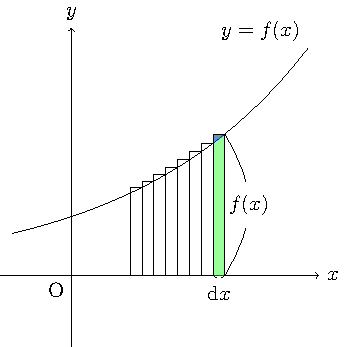
\includegraphics[width=5.5cm]{picture/sekibun1.pdf}
 \caption{積分は面積を表す}
  \label{fig:sekibunmenseki}
\end{figure}

$f(x) \: \mathrm{d}x$という部分が図の緑で塗った部分と青で塗った部分の面積の合計で,
``真の''面積が図の緑で塗った部分の面積である.
これらがほとんど違わないのがわかるだろう.もしも幅$\mathrm{d}x$をもっと小さくとれば,両者の差はもっと小さくなる. 
さらに,$\mathrm{d}x$を一種の理想的なごくごく微小な幅とすれば,もはや両者は完全に一致しているとみなしてよいだろう.
この小さい短冊状の図形の面積を区間$[a, \, b]$全域にわたって合計するのだ.
これが曲線$y=f(x)$,2直線$x=a$,$x=b$,および$x$軸で囲まれる図形の面積に等しいというのも納得がいくだろう.
ただし,$f(x)$は常に正の値をとるとは限らない.負の値をとることだって考えられる.
このとき,面積は負の値となってしまうので,定積分によって得られた値を
\emph{符号付き面積}\index[widx]{ふごうつきめんせき@符号付き面積}と呼ぶことにしよう.

これで定積分のおおまかなイメージはついただろう.``積分は微分の逆演算である''という解釈については何も説明してないが,
とりあえず後回しにさせてもらうことにして,定積分の正確な定義を書いておこう.
\subsubsection{定積分の正確な定義}
区間$[a, \, b]$で定義された有界な関数$f(x)$を考える.有界というのは大雑把に言えば
関数の値が途中で無限大に発散してしまうことはないくらいのイメージである.
和をとるときに無限大なんてものが混ざっていると足し算がうまくいかないので,そういう可能性を排除してあるのである.
そして,区間$[a, \, b]$を$n$個の小区間に分割するような分割$\varDelta$を考える.
\begin{equation*}
\varDelta : x_0 = a < x_1 < x_2 < \cdots < x_{n-1} < x_n =b
\end{equation*}
ここで重要なのが分割する,と言っているだけで等分とは一言も言っていない点である.どんな変な分割でもかまわない.
さらに,$\varDelta x_i = x_i - x_{i-1}$とおく.これは分割した各小区間の幅である.各小区間から点$c_i$を任意にとり,次のような和を考える.
\begin{equation*}
\sum_{i=1}^{n} f(c_i) \varDelta x_i
\label{riemannwa}
\end{equation*}
これがいわゆる$f(x)$の区間$[a, \, b]$における$f(x)$の\textbf{Riemann和}
\index[widx]{Riemannわ@Riemann和}
\index[nidx]{Riemann@Riemann(リーマン)}と呼ばれるものである.
ここで,各小区間の幅を限りなく小さくしてやる.
1つの式で書きたければ,$\varDelta x_i$の
最大値$\delta = \max \{ x_i-x_{i-1} \} $が限りなく小さくなるとでも書いてやればいい.
もちろん$n$が限りなく大きくなると考えても同じことである.
つまり,次のような極限を考えるのである.
\begin{equation*}
\lim_{\delta \to 0} \sum_{i=1}^{n} f(c_i) \varDelta x_i
\end{equation*}
この極限が分割$\varDelta$や$c_i$のとり方に依存せず,一定の値に確定するとき,関数$f(x)$は区間$[a, \, b]$で
\emph{可積分}\index[widx]{かせきぶん@可積分}であるといい,その極限値を
\begin{equation*}
\int_a^b f(x) \; \mathrm{d}x
\end{equation*}
と書く.そして,この極限値を求める操作を``定積分する''と呼ぶのである.

先ほどの直感的な説明とうまく対応しているのがわかるだろうか? $\Sigma$が$\int$に,
$\varDelta x_i$が$\mathrm{d}x$に,$c_i$が$x$に対応しているのである.

分割だの$c_i$だのは数学者が定義を正確にするために導入したいわば技巧的なものに過ぎない.
この技巧がどんなものかを学ぶことは非常に重要なことであるが,物理学の参考書という体裁上,
深入りするのはやめておくことにする.興味があれば勉強してみるのもいいだろう.

ただし,何が目的でこのような定義をしたかは知っておく必要がある.
この定義には面積などといった幾何学的な\footnote{ざっくりいうと図形的なという意味である.}要素は一切含まれていない.
面積はあくまで積分の解釈の1つに過ぎないのである.

そこで,面積というものを積分でもって定義することができるのである.
面積というものは今まであいまいなままであったが,これを積分でもって厳密に定義できるのである.
このあたりの話をもっと詳しく知るためには
$\varepsilon-\delta$論法を学ばなければならない.
後回しにすると面倒な理論なので興味があったら早めに学ぶとよい.
とっかかりは大変かもしれないが,そこから先は驚くほど単純である.
ただし,受験数学に毒されてしまった人にとっては難しいかもしれない.
\subsection{不定積分}
今までの説明では,積分と微分が互いに逆演算であるというイメージは出てこなかった.
積分とは無限個足し算であるという解釈なのであった.だが,そういう解釈をしたところで,
実際にそれを計算するのは非常に難しい.これでは積分はあまり役に立たない理論であったことだろう.
現実でそうなっていないのは微分と積分という一見関係なさそうに見える2つの概念が
実は深くかかわっていることが明らかになったからである.
この事実は微分積分学の基本定理
と呼ばれるもので,発見者はNewton\index[nidx]{Newton@Newton(ニュートン)}と
Leibniz\index[nidx]{Leibniz@Leibniz(ライプニッツ)}であり,互いに相手の研究内容は知らなかった. 
彼らが微分積分学の創始者であるといわれるのはこのことが理由になっているのである.
2人はほぼ同時期にこの定理を発見した.そのためかNewtonの支持者が
Leibnizをパクリだとひどく批判したが,Leibnizも自身の独創性を譲ろうとはしなかった.
もちろん微分積分学の理論は双方とも単独で作り上げたものであり,どちらがパクリなどということはない.

寄り道はこの辺にしておいて本題に戻るとしよう.定積分の話をするときに,積分には2種類あると言った.
1つはさっき説明した定積分であるが,
もう1つがこれから説明する不定積分である.

連続関数$f(x)$に対し,微分したら$f(x)$になるような関数$F(x)$があったとする.
\begin{eqnarray}
F'(x) = f(x)
\label{eq:ghuteisekibun}
\end{eqnarray}
ということである.この関数$F(x)$を$f(x)$の\emph{原始関数}\index[widx]{げんしかんすう@原始関数}と呼ぶ.
原始関数は無数に存在する.関数$f(x)$の原始関数$F(x)$が1つ存在すれば,それに定数$C$を加えた関数
$F(x)+C$も$f(x)$の原始関数だからである.これらをすべてまとめて
$$
\int f(x) \, \mathrm{d}x
$$
と書き,これを$f(x)$の\emph{不定積分}\index[widx]{ふていせきぶん@不定積分}と呼ぶ.
\begin{eqnarray}
\int f(x) \, \mathrm{d}x = F(x) + C \;\; (\text{ただし} F'(x)=f(x))
\label{eq:huteisekibun}
\end{eqnarray}
ということである.定積分のときと記号が似通っているのは微分積分学の基本定理があるからである.
両者のイメージはまったくの別物であるということには注意しなければならない.
不定積分の計算法は普通の数学書であれば必ず載っているのだが,今の目的は積分とは何なのかを知ることにあるので
とっとと先に進むことにする.
微分と積分がつながっているという事実を述べたのが次の定理である.
\begin{itembox}[l]{微分積分学の基本定理}
$a$を定数,$f(x)$を連続関数として,$x$の関数
$$
\int_{a}^{x} f(x) \, \mathrm{d}x
$$
は$f(x)$の原始関数である.つまり,
$$
\frac{\mathrm{d}}{\mathrm{d}x}\int_{a}^{x} f(x) \, \mathrm{d}x = f(x)
$$
となる.
\end{itembox}
積分して微分したら元に戻ってくるということは,微分と積分が互いに逆の演算であると言わざるを得ないだろう.

微分積分学の基本定理は別の表現もできる.
\begin{itembox}[l]{微分積分学の基本定理の別表現}
連続関数$f(x)$の任意の原始関数$F(x)$に対し,
$$
\int_{a}^{b} f(x) \, \mathrm{d}x = F(b)-F(a)
$$
となる.
\end{itembox}
ここでは,これらの定理の証明はしない.厳密に,正確に理解したければやはり$\varepsilon - \delta$論法を学ばなければならないからだ.
定積分の解説の最後の部分で述べた疑問への回答がこの定理である.定積分をしたければ,対象の関数の原始関数
を求めてやり,その変化量を計算してやればよいということである.
原始関数を求めることはときどき非常に面倒なケースに出くわすことがあるが,それでも``無限個の足し算''を実行するよりも
はるかにマシである.

また,高校ではこれが定積分の定義として扱われている.無限個の足し算というものが高校の範囲ではうまく説明できないからであろう.
しかし,それでは積分の本質にたどり着くことはできない.
この定義でもあまり問題はないのだが,面積というものが相変わらずあいまいなままになってしまう.
大学での積分論がよく理解できないのはこのあたりの事情が原因になっているのだと思う.
定義が変われば混乱するのも当たり前である.
\footnote{もしかしたら,高校生の間には定義は``神様''が決めるもので,
変えることは許されないという雰囲気が蔓延しているのかもしれない.}

最後に1つ補足をしておく.私はさっきまでずっと``定積分と不定積分のイメージはまったく違うものである''
と言ってきたが,よくよく考えてみるとそうでもないのである.
定積分のところで$f(x) \, \mathrm{d} x$というものが出てきた.
この形式,どこかで見たことはないだろうか? なんと,
この量は$f(x)$の原始関数の微分になっているではないか!
$f(x)$の原始関数の1つを$F(x)$としてみれば,$F(x)$の微分は
\begin{align*}
\mathrm{d}F = F'(x) \, \mathrm{d}x = f(x) \, \mathrm{d} x
\end{align*}
であるからだ.
この量をある範囲にわたって足し合わせていくのが定積分であった.$\mathrm{d} F$を連続した区間$[ a, \, b ]$で
足し合わせてみれば,はしっこ以外の値は打ち消されあって結局$F(b) - F(a)$しか残らない.
このことを確かめるのは読者にゆだねることにしよう.けっこういろいろと仮定を敷いていることに気が付くはずだ.
例えば$F(x)$の値が急激に激しく変化することはないとかそういうものである.
そして,そうして無限個の足し算を実行した結果は$\int$記号を用いて
\begin{align*}
\int_{F(a)}^{F(b)} \, \mathrm{d} F
\end{align*}
と書くのであった.
\footnote{表記の都合上積分範囲が変わっているが,とりあえず気にしなくてよい.}
ここではこの結果が$F(b)-F(a)$であったから
\begin{align*}
\int_{F(a)}^{F(b)} \mathrm{d}F = F(b) -F(a)
\end{align*}
である.最後に$\mathrm{d}F$は$f(x) \, \mathrm{d} x$だったのでこれを代入すると
\begin{align*}
\int_a^b f(x) \, \mathrm{d}x = F(b) - F(a)
\end{align*}
という式が得られたことになる.
これは微分積分学の基本定理ではないか! 微分と積分はこういうロジックでつながっているのである.
もちろん,こんなものは証明と呼べるようなものではない.
``無限個の足し算''や``微小''などといった概念はもっと慎重に扱わなければならないものである.
多くの物理数学の本では,
そのなかで正しいことが数学者のたゆまぬ努力によって証明されたものだけを都合よく拾ってきているのである.
詳しく知りたければやはり,$\epsilon - \delta$論法を学ぶべきである.
 % 積分
\chapter{多変数関数の微積分}
さっきまでやってきたのは,1変数関数に関する微分積分学である.
しかし,物理量は1つの変数で決められるようなものはあまりない.変数が足りないのである.
複数の数に対して1つの数を対応させるような対応関係のことを\emph{多変数関数}
\index[widx]{たへんすうかんすう@多変数関数}というのだが,
この多変数関数に関しても微分積分学を考えたい.しかし,たくさんある変数のうちどれを追いかけたらいいのかよくわからない.
というわけで,まずは1つの変数にのみ着目し,あとの変数は定数だとみなしてしまうことにしよう.
このときに使うのが偏微分である.
偏微分を学ぶ前に,とりあえず多変数関数について確認しておこうか.
\section{多変数関数}
おそらく,読者の方々が高校生の間に扱ってきたのは独立変数を1つだけ持つ1変数関数である.
高校までの物理で扱ったのもおそらく1変数関数だけである.
時間$t$での物体の位置$x(t)$だとか,位置$x$での物体のポテンシャルエネルギー$V(x)$などがあっただろう.
しかし,物理量を扱ううえで,これではまずいのである.
例えば熱力学では,ある系の圧力$p$は,その系の体積$V$と温度$T$を決めてしまえばただ1通りに定まる.
だが,体積だけ,あるいは温度だけを決めても圧力は決まらない.
関数と似ているだろう.この場合,圧力は温度と体積の関数ということになる.
圧力$p$は$p(V, \, T)$と表せるのである.
この例では独立変数が2つある.温度と体積はそれぞれ勝手に動く.
一方,例えば温度を決めたとしても,それによって体積に何らかの制限がかかることはない.
``独立''変数というのはそういう意味である.
電磁気学での例も出しておこう.例えば,空間の電荷密度$\rho$は,位置と時間を決めれば値が決まる.
こういうと変数が位置と時間の2つのように聞こえるが,実際は4つの独立変数を持つ.
それは,位置が3つの変数によって決まるからだ.$x$座標,$y$座標,$z$座標を決めねば位置は決まらない.
だが,位置を決めれば電荷密度が決まるといえるかといえばそうではない.
ある場所の,基準の時間から1秒経ったときの電荷密度と3秒経ったときの同じ場所での電荷密度は同じとは限らない.
空間の電荷が移動していれば,電荷密度は時間とともに変化するからだ.
電荷密度は$x, \, y, \, z$そして時間$t$の4変数関数であるというわけだ.

さて,多変数関数の概念が何となく理解できたところできちんと定義しておこう.
$n$個の数$ x_1, \, x_2, \, \cdots , \, x_n $の値が確定したとき,もう1つの数$y$の値が
ただ1つに確定するような対応規則が与えられたとき,
そのような対応規則のことを\textbf{$n$変数関数}と呼ぶ.
\emph{多変数関数}\index[widx]{たへんすうかんすう@多変数関数|textbf}というのは,
値を決めるのに2つ以上の独立変数の値を要求する関数のことである.
そして,最初に決める変数(ここでは$ x_1, \, x_2, \, \cdots , \, x_n $のこと)を\emph{独立変数}
\index[widx]{どくりつへんすう@独立変数},
独立変数に対応して決定される変数(ここでは$y$のこと)を\emph{従属変数}
\index[widx]{じゅうぞくへんすう@従属変数}という.
$n$変数関数のことをよく$f$という記号で表すことが多い.
そして,独立変数の値を$ x_1, \, x_2, \, \cdots , \, x_n $に決定したとき,これらの数に対応する従属変数の値を
\begin{align*}
f( x_1, \, x_2, \, \cdots , \, x_n)
\end{align*}
と表す.
もし$x_1, \, x_2, \, \cdots , \, x_n$に対応する従属変数が$y$と表されていれば,それは
\begin{align}
y = f(x_1, \, x_2, \, \cdots , \, x_n)
\label{eq:nhensu}
\end{align}
というように表されるのである.
特に,2変数関数のときには独立変数を$x, \, y$と書き,従属変数を$z$と書いて
\begin{align}
z = f(x, \, y)
\label{2hensu}
\end{align}
と表すことが多く,3変数関数の場合には独立変数を$x, \, y, \, z$と書き,従属変数を$u$と書いて
\begin{align}
u = f(x, \, y, \, z)
\label{eq:3hensu}
\end{align}
と書き表すことが多い.また,対応関係を表す記号(ここでは$f$としている)は使わずに,
直接$z(x, \, y)$や$u(x, \, y, \, z)$と表してしまうことも多い.
ここで注意しなければならないのは,
独立変数や従属変数を表すのに使っていた記号はあくまでシンボルであるということである.
関数というのは数(2変数以上の場合には数の組)と数との対応規則であって,
$y$だの$x$だのといった文字で表された具体的な式のことではないのである.
\footnote{実は,このような解釈に至ったのはけっこう最近のことだったりする.}
とはいえ,やっぱり厳密に区別するのもめんどくさいので
``2変数関数$f(x, \, y)$''だとか``関数$u(x, \, y,\, z)$''などというようにといってしまうことも多い.
普通の本だとこういう表記はたくさんあるはずだ.本書にもたくさんある.

\begin{itembox}[l]{検討}
さっきまで書いていた関数の定義は,中学校や高校の教科書に書いてあるような定義とは少し違うはずである.
君たちの家にある中学校や高校の数学の教科書に書いてある関数の定義を調べ,
本書に記した定義と何がどう違うかをまとめよ.
\end{itembox}
物理をやるうえでは関数が数(の組)と数との対応規則であることを知らなくともどうにかなることが多いのだが,
やはり自分がよく使っているものの正確な定義くらいは知っておきたいものである.
\footnote{ここで,対応規則という言葉がひどく曖昧に思えたら一人前といっていいだろう.}
\newpage
\subsubsection{2変数関数のグラフは曲面を表す}
1変数関数$f(x)$において,実数$x$とそれに対応する値$f(x)$のペア$(x, \, f(x))$全体の集合は,
このペアを点の座標と考えることにより,曲線とみなせるのであった.
$x$軸上の各点$(x, \, 0)$に対して$f(x)$という高さを対応させ,
それを平面上に図示したのが図\ref{fig:f(x)}である.
\begin{figure}[h]
 \centering
 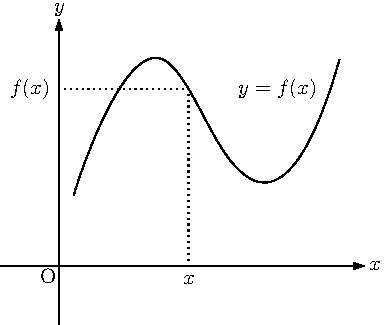
\includegraphics[width=5.8cm]{picture/henbibun1.pdf}
 \caption{1変数関数$y=f(x)$のグラフ}
 \label{fig:f(x)}
\end{figure} 

もちろん,$(x, \, f(x))$というペア全体の集合が曲線とみなせるのは,
$f$がなにかしらの良い性質を持っているときだけなのであるが,
物理で扱う関数はほとんどが滑らかさというとても良い性質を持っていることが多い.
あんまり細かいことは気にする必要はないということだ.

次に,2変数関数$f(x, \, y)$について考えよう.2つの実数$x, \, y$とそれに対応する値$f(x, \, y)$のペア
$(x, \, y, \, f(x, \, y))$を座標と解釈すれば,このペア全体の集合は曲面を表すことになる.
$xy$平面上の各点$(x, \, y, \, 0)$に対し,$f(x, \, y)$という高さを対応させていると考えるのである.
このことを空間上に図示したのが図\ref{fig:f(x,y)}ということになる.
\newpage
\begin{figure}[h]
 \centering
 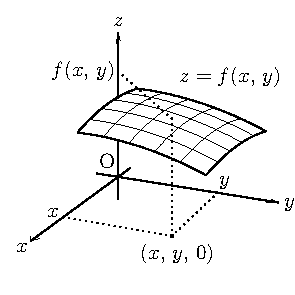
\includegraphics[width=5.8cm]{picture/henbibun2.pdf}
 \caption{2変数関数$z=f(x, \, y)$のグラフ}
 \label{fig:f(x,y)}
\end{figure} 
この場合も曲面とはとても思えないような変な関数を用意することもできるのだが,
話がややこしくなるのでそういうことはやめておくことにする.

この調子で3変数以上の関数についても考えることができそうだが,
3変数関数のグラフは4次元空間に存在するものであり,
これを人間の目に見える形で図示するのは不可能である.
\footnote{世の中には4次元空間が``見える''人が存在するようである.}
\subsection{陰関数}
関数というのは2つの量の関係を表すのであったが,どんな関係でも表せるというわけでもなく,
独立変数の値が決定されれば従属変数の値がただ1つに決定されるというような関係しか表せないのであった.
\footnote{しかし,従属変数の値が決定されても独立変数の値がただ1つに決定される必要はない.}
1変数関数のグラフは平面曲線を表し,2変数関数のグラフは空間曲面を表すのだが,
逆に,平面上の曲線すべてを1変数関数で表すことはできないし,
空間の曲面すべてを2変数関数で表すことはできない.
円や球面といった図形を考えてみればわかるはずだ.

このような曲線,曲面は単に$x, \, y$もしくは$x, \, y, \, z$の方程式として表される.
円であれば方程式$x^2+y^2=r^2$,球面であれば方程式$x^2+y^2+z^2=r^2$というようになるのである.
場合によっては1つの図形を表すのに方程式が複数必要になることがある.
例えば空間に存在する直線を表す場合である.詳細は高校レベルであるから省かせてもらう.

結局のところ,平面上の曲線や空間上の曲面は,$f(x, \, y)=0$
や$f(x, \, y, \, z)=0$といった方程式の形で表せるのである.
この$f$は今度こそ関数である.よく見ると,曲線を表す場合には$f(x, \, y)=0$となり,
この方程式は曲面を表していた
2変数関数$z=f(x, \, y)$に対して$z=0$という条件を付け加えたものと解釈できる.
曲面の場合も同様である.

さて,方程式が与えられればそれを解くことができるであろう.
話を簡単にするためにも平面上の曲線が方程式$f(x, \, y)=0$で表されている場合について考えよう.
いま,方程式$f(x, \, y)=0$が与えられたとき,それを$y$について解けば$y=g(x)$という形になることが予想される.
しかしこの$g$は関数であるとは限らない.方程式の解は複数存在し得るからだ.
だが,この方程式の解をたった1つの関数で表そうとしたのがいけないのであって,
複数の関数を用いて表してみてはどうだろう.
複数の関数を用意すれば方程式$f(x, \, y)=0$の定める$x$と$y$の関係を
完全に再現することができるはずである.
それに加え,もし大域的に見て解が複数あったとしても,$x$や$y$の値を制限して局所的に考えれば,
$y$を$x$の関数としてただ1通りに表すことができることが知られている.
局所的には方程式$f(x, \, y)=0$の解は1つしかないということである.
\footnote{この事実は数学的にも重要であって,陰関数定理と呼ばれている.}
すなわち方程式{$f(x, \, y)=0$}で表されるような曲線は,
複数の関数をひとまとめにしたものであるとみなせるのである.

きちんと定式化しておこう.2つの変数$x, \, y$について,方程式$f(x, \, y)=0$
が与えられたとする.この方程式が定める曲線上の点$(a, b)$の十分近くにおいて,
この曲線がある1変数関数$g$を用いて$y=g(x)$のグラフであるとみなせるとき,
すなわち,$a$に十分近い任意の$x$に対して$f(x, \, y)=0$をみたす$y$がただ1つに定まるとき,
この対応関係$g$は点$(a, \, b)$近傍において定義される関数である.
このとき,$g$は方程式$f(x, \, y)=0$によって
\emph{陰伏的に定められる}といい,
$g$を方程式$f(x, \, y)=0$によって定められる
\emph{陰関数}\index[widx]{いんかんすう@陰関数}と呼ぶ.
また,方程式$f(x, \, y)=0$が定める陰関数が複数あるとき,
それぞれの陰関数のことをこの陰伏関数の\emph{分枝}\index[widx]{ぶんし@分枝}と呼ぶ.
曲線を複数の枝の集まりだとみなしたときに,それぞれの枝が陰関数だと思ってのネーミングである.

これに対し,通常の$y=f(x)$の形の関数のことを\emph{陽関数}\index[widx]{ようかんすう@陽関数}と呼ぶことがある.
この対応関係は明らかに(陽に)関数ですよという意味合いを強調したいのだろう.

\subsection{パラメータ表示}
さて,陰関数の次はパラメータ表示の話である.
``パラメータ''という言葉は聞いたことくらいはあるだろう.
パラメータという言葉は学問分野や文脈,\index[widx]{ぱらめーた@パラメータ}
果ては個人個人によって異なる意味合いで使われることがあり,
正確に定義しろと言われてもちょっと難しいものがある.
とはいえ,みんな好き勝手に使っているのかというとそうでもなく,
たいていは「考えている対象の何らかの特性を表す補助的な変数」くらいの意味で使っていることが多い.
これから話すのは``曲線・曲面のパラメータ表示''という文脈で一般に使われているパラメータの話である.

\subsubsection{曲線のパラメータ表示}
さてと,まずは曲線について考えよう.平面上にある曲線$C$を考える.
話を簡単にするためにも,$C$はある点Aから別の点Bを連続的に繋いだ曲線だとしよう.
ある点Pを,点Aから出発して曲線$C$に沿って点Bまで動く点であるとしよう.
どのくらい動いたかは何らかの変数$t$によって定められているとしておく.
$t$が$a$から$b$まで動くとすれば,$t=a$ではPはAと一致し,$t=b$ならPはBと一致し,
$t$が増加するにしたがってPが曲線$C$上をAからBに向かって動いていくようなイメージである.
このとき,$t$が決まれば点Pがどこにあるかが確定する.
すなわち,点Pの座標は$t$の関数(っぽいもの)であるといえるのである.
平面上の点の座標というのは$x$座標と$y$座標で構成されるのだから,
点Pの座標が$t$で決まるというのは
Pの$x$座標と$y$座標がともに$t$の関数であるということと同値である.
その関数を$\varphi, \, \psi$としてみよう.
すなわち,点Pの座標を$(x, \, y)$としたときに,
\begin{align}
\left\{
\begin{aligned}
x & = \varphi(t) \\ 
y & = \psi (t) 
\end{aligned}
\right.
\qquad ( \, a \leq t \leq b \, )
\label{eq:parameta}
\end{align}
となるということである.
\footnote{本書では,不等号として$\leq, \, \geq$を採用している.
これらはそれぞれ$\leqq, \, \geqq$と同じ意味である.}
これを見ると,曲線$C$の各点$(x, \, y)$に対し,$a \leq t \leq b$なる実数$t$が
完全に1対1対応している.
\footnote{本当は$C$の端点などで1対1対応が崩れていても構わない.
この場合の点Aと点Bが一致する\emph{閉曲線}\index[widx]{へいきょくせん@閉曲線}の場合
などでこういうことが起こりうる.}
すなわち,式(\ref{eq:parameta})は曲線$C$を完全に表しているものといえる.
この実数$t$は曲線の形に何の影響も与えない.
重要なのは関数$\varphi, \, \psi$の形の方である.
すなわち,この$t$は曲線$C$を表すためのいわば補助的な変数といえるわけだ.
この$t$が冒頭に書いたパラメータの意味合いに合致していることがわかるだろう.
そういうわけで,式(\ref{eq:parameta})のことを$C$の
\emph{パラメータ表示}\index[widx]{ぱらめーた@パラメータ!ひょうじ@---表示}だとか
$C$の\emph{パラメトリック方程式}\index[widx]{ぱらめとりっくほうていしき@パラメトリック方程式|see{パラメータ}}
などと呼ぶ.
いまこの意味で使っているパラメータ(parameter)は
日本語では\emph{媒介変数}\index[widx]{ばいかい@媒介変数|see{パラメータ}}と訳される.
そういうわけで,高校の教科書なんかでは式(\ref{eq:parameta})のことを
$C$の\emph{媒介変数表示}
\index[widx]{ばいかいへんすう@媒介変数!ひょうじ@---表示|see{パラメータ}}と呼ぶのが普通である.

今回は曲線$C$が有限の範囲に収まっている状況を想定したが,
別にそうである必要もあるまい.パラメータの範囲を無制限にしてやれば,
はるか遠方にある$C$の点だって表現できるだろう.
今回そういう場合を考えなかったのは,はるか遠方まで曲線が伸びることを許すと,
どこを始点に据えたものかよくわからなくなるからである.
これは単に説明がしづらいということ以上の理由はない.
パラメータ表示ができるのは有限の範囲に収まった曲線だけだと勘違いしないように.

曲線のパラメータ表示はとても便利である.
まず,曲線上の点を考えるのに$t$という仮変数を用いることにより,
曲線を表す方程式が簡単に書けたりする.
これは,あとで実例を見せることにしよう.
次の点が最も重要であり,
さっきまではパラメータになにか特別な意味は持たせていなかったが,
あえてパラメータになんらかの意味を与えてやることにより,
具体的なイメージが容易になったり,そこに隠された性質が見えてきたりするのである.
これも実例を挙げて説明するのがいいだろう.次のパラメータ表示を見てほしい.
\begin{align*}
\left\{
\begin{aligned}
x & = v_0 \cos \theta \cdot t \\
y & = v_0 \sin \theta \cdot t - \frac{1}{2} g t^2 
\end{aligned}
\right.
\qquad ( \, 0 \leq t \, )
\end{align*}
ここで,$v_0, \, \theta , \, g$はただの定数であり,変化するのは$t$のみである.
もはやこの$t$が何を表していると解釈するかなどという野暮な問は不要だろう.
$t$を時間として解釈するのが自然である.
もちろんパラメータを消去して,
\begin{align*}
y = \tan \theta \cdot x - \frac{ g } { 2 v_0^2 \cos ^2 \theta} x^2
\end{align*}
と書くこともできるが,$t$を時間として解釈した以上,
この式は斜方投射を表していると理解しやすいのはパラメータ表示された式の方であろう.

\subsubsection{曲面のパラメータ表示}\index[widx]{ぱらめーた@パラメータ!ひょうじ@---表示}
次は,曲面のパラメータ表示についてである.
空間に存在する曲面$S$について考える.
曲線のときと同じように考えるとちょっと説明が面倒になるので,
今回は違った方法で考えてみよう.

$S$は空間に存在する曲面である.$S$の各点$(x, \, y, \, z)$に対し,
その点から$xy$平面に降ろした垂線の足全体の集合を$\pi$とおく.
\footnote{この集合$\pi$を$S$の$xy$平面への正射影という.}
\index[widx]{せいしゃえい@正射影}
$\pi$上の各点はすべて$xy$平面上の点だから,その座標$(x, \, y, \, 0)$
は2つのパラメータで表されるはずだ.
\footnote{$\pi$は曲線の無限個の和集合とみなせるから,
1つ目のパラメータでその点が$\pi$のどの曲線上にあるか指定し,
2つ目のパラメータでその点が曲線上のどこにあるかを指定するような
イメージをしてみれば納得できるだろう.}
そこでそのパラメータを$u, \, v$として,関数$\varphi, \, \psi$を用いて,
\begin{align*}
x = \varphi (u, \, v) \\
y= \psi (u, \, v)
\end{align*}
と表そう.なんでわざわざ平面上の点を$u, \, v$というパラメータを用いて表すのかといえば,
その方が後で楽だからである.
後の話を楽に進めるために,
$u, \, v$の組$(u, \, v)$と$\pi$上の各点$(x, \, y)$は完全に1対1対応している必要はないとしよう.
異なる2つの$u, \, v$の組$(u, \, v)$が$\pi$上の同じ点に対応させてもいいとするのである.

さて,$\pi$上の点が決まったとき,
その点と$x$座標と$y$座標が同じであるような$S$上の点を考える.
$\pi$上の各点に対し,その点と$x$座標と$y$座標が同じであるような$S$上の点は
ただ1つしかないといいたくなるが,いま,$S$は任意の曲面である.
そのため,$\pi$上の点を1つ決めても,その点と$x$座標と$y$座標が同じであるような
$S$上の点が複数ある場合があるのである.
この問題をパラメータが解決してくれる.
$\pi$上の各点に対し,その点と$x$座標と$y$座標が同じであるような$S$上の点
が複数あったとき,その数だけ異なるパラメータの組$(u, \, v)$に対して
同じ$\pi$上の点を対応させるとしよう.
そう考えれば,$S$上の点の$z$座標は$u, \, v$の関数として表すことができるのである.
そこでこの関数を$\xi$として,
\begin{align*}
z = \xi (u, \, v)
\end{align*}
と表すことにしよう. まとめると,$S$上の各点$(x, \, y, \, z)$は$u, \, v$という2つのパラメータを用いて
\begin{align}
\left\{
\begin{aligned}
x & = \varphi (u, \, v) \\
y & = \psi (u, \, v) \\
z & = \xi (u, \, v)
\end{aligned}
\right.
\label{eq:kyokuparameta}
\end{align}
と表せるのである.
これが曲面$S$のパラメータ表示である.
曲線から曲面になったときに,必要なパラメータが1つ増えたのである.

なお,空間に存在する曲線は,やはり1つのパラメータで
\begin{align}
\left\{
\begin{aligned}
x & = \varphi (t) \\
y & = \psi (t) \\
z & = \xi (t)
\end{aligned}
\right.
\end{align}
とパラメータ表示される.なぜかはもはや説明するほどでもないだろう.

長かったが,言いたいことは曲線はパラメータ1つで,
曲面はパラメータ2つでパラメータ表示できるということだけである.

\subsubsection{パラメータ表示された曲線の概形を描く}
さて,ここまで一般的な話しかしてこなかったので,
何か具体例が欲しいところである.
そこで,微分法の復習もかねて,パラメータ表示された曲線の概形を描いてみよう.

$a$を正の定数として,
$xy$平面上の曲線$C$が以下のようにパラメータ表示されているとする.
\begin{align}
\left\{
\begin{aligned}
x & = a ( 1 + \cos t) \cos t \\
y & = a ( 1 + \cos t ) \sin t
\end{aligned}
\right.
\qquad (0 \leq t \leq 2 \pi)
\label{eq: cardioid}
\end{align}
この曲線$C$を図示してみよう.
そのためにも,$t$の変化に対して$x, \, y$がどのように変化するかが知りたいところである.
すなわち,$t$に対する,$x, \, y$の変化率が知りたいのである.
それには,$x, \, y$を$t$で微分してやればいい.
\begin{align*}
\frac{ \mathrm{d} x} { \mathrm{d} t} 
& = a \cdot \Big( -\sin t \cos t + (1+ \cos t) (- \sin t) \Big) \\
& =  -a \sin t (1 + 2 \cos t) \, , \\
\frac { \mathrm{d} y} { \mathrm{d} t} 
& = a \Big( -\sin t \sin t + (1 + \cos t) \cos t \Big) \\
& = a ( 2 \cos ^2 t + \cos t -1) \\
& = a (\cos t +1) (2\cos t -1)
\end{align*}
今求めたのは$x, \, y$の$t$に対する変化率である.
従って,この値が正であれば$t$の増加に対して$x, \, y$は増加し,
負であれば$t$の増加に対して$x, \, y$は減少する.
もし0であれば$t$がほんの少し変化しても$x, \, y$の値は変化しないということになる.
これをもとに,$t$に対する$x, \, y$の変化を表にまとめよう.
このような表は$t$に対する$x, \, y$の\emph{増減表}\index[widx]{ぞうげんひょう@増減表}
と呼ばれるのであった.

\begin{table}[h]
\renewcommand{\arraystretch}{1.6}
\begin{flushleft}
\begin{tabular}{|c||c|c|c|c|c|c|c}
\hline
$t$ & 0 & $\cdots$  & $ \displaystyle \frac{ \pi }{3} $ & $\cdots$ 
& $ \displaystyle \frac{2}{3} \pi $ & $\cdots$ & \hspace{0.1cm} $\pi$ \hspace{0.1cm} \\ \hline
$ \displaystyle \frac{\mathrm{d} x }{\mathrm{d} t} $ & (0) & \multicolumn{3}{c|}{$-$} & 0 & $+$ & 0 \\ \hline
$x$ & $2a$ & $\leftarrow$ & $\displaystyle \frac{3}{4} a$ & $\leftarrow$ 
& $\displaystyle - \frac{1}{4} a$ & $\rightarrow$ & 0 \\ \hline
$\displaystyle \frac{\mathrm{d} y }{\mathrm{d} t}$  & (0) & $+$ & 0 &\multicolumn{3}{|c|}{$-$} & 0 \\ \hline
$y$ & 0 & $\uparrow$ & $ \displaystyle \frac{ 3 \sqrt{3} }{4} a$ & $\downarrow$ 
& $\displaystyle \frac{\sqrt{3} }{4} a$ & $\downarrow$ & 0 \\ \hline
\end{tabular}
\end{flushleft}
\end{table}
\vspace{-0.5cm}
\begin{table}[h]
\renewcommand{\arraystretch}{1.6}
\begin{flushright}
\begin{tabular}{c|c|c|c|c|c|}
\hline
$\cdots$ & $ \displaystyle \frac{4}{3} \pi$ & $ \cdots $ 
& $ \displaystyle \frac{5}{3} \pi $ & $ \cdots $ & $ 2 \pi $ \\ \hline
$-$ & 0 & \multicolumn{3}{c|}{$+$} & (0) \\ \hline
$\leftarrow$ & $ \displaystyle - \frac{1}{4} a$ & $\rightarrow$ 
& $ \displaystyle \frac{3}{4} a$ & $\rightarrow$ & $2a$ \\ \hline
\multicolumn{3}{c|}{$-$} & 0 & $+$ & $(+)$ \\ \hline
$\downarrow$ & $\displaystyle -\frac{ \sqrt{3}}{4} a $ & $\downarrow$ 
& $ \displaystyle -\frac{3\sqrt{3}}{4} a $ & $\uparrow$ & 0 \\ \hline
\end{tabular}
\end{flushright}
\end{table}
この表の意味はわかるだろう.$x$が増加・減少は$x$軸を歩くようなイメージで横向きの矢印で表しており,
$y$の増加・減少は$y$軸を歩くようなイメージで縦向きの矢印で表している.
この表から曲線$C$の概形がイメージできるだろうか? $t=0$に対応する点$(2a, \, 0)$からスタートして,
そこから$t$の増加に伴い増減表に書いたような進み方で進んでいく.
そうして最終的に$t= 2 \pi$に対応する点$(2a, \, 0)$に戻ってくるというわけである.
このことを頭に思い浮かべながら$C$の概形を描けば,
それは図\ref{fig:cardioid}のようになる.

\begin{figure}[h]
 \centering
 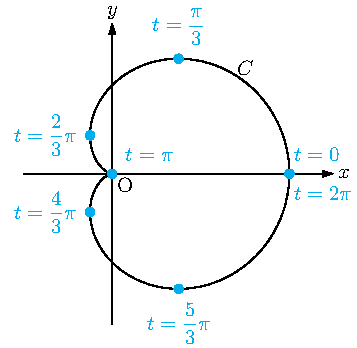
\includegraphics[width=5.5cm]{picture/henbibun3.pdf}
 \caption{曲線$C$の概形}
 \label{fig:cardioid}
\end{figure}

$x, \, y$の増減が変化する点とそのときの$t$の値を図に書き込んでおいた.
あまりたくさん情報を書き込みすぎると図が汚くなるので書き込む情報は最小限に抑えている.
ここまで書かれればさすがに理解できるだろう.

この曲線は\emph{カージオイド}\index[widx]{かーじおいど@カージオイド}と呼ばれる有名な曲線である.
名前くらいは聞いたことがあるかもしれない.
\begin{itembox}[l]{課題}
\begin{align*}
\left\{
\begin{aligned}
x & = a ( t - \sin t) \\
y & = a ( 1 - \cos t )
\end{aligned}
\right.
\qquad (0 \leq t \leq 2 \pi)
\end{align*}
とパラメータ表示された曲線の概形を描け.
ただし$a$は正の定数とする.
 \end{itembox}
なお,この曲線もこれまた有名な曲線で,\emph{サイクロイド}\index[widx]{さいくろいど@サイクロイド}
と呼ばれている.
物理を学んでいると,時々出くわすことがある曲線である.
名前くらいは覚えておいても損はないだろう.
\section{偏微分}
ここからやっと偏微分の話に入る.
多変数関数なら変数がいくつあってもここから先の話はまったく変わらないのだが,
ここは簡単のために3変数関数について考える.
$x, \, y, \, z$の3つの独立変数をもつ関数$f(x, \, y, \, z)$について考えよう.
この関数$f$というのは,$x, \, y, \, z$の3つの値を定めたときに
初めて$f(x, \, y, \, z)$という値が定まるような対応関係であった.
そこで,先に$y=b, \, z=c$と定めてしまおう.$x$の値がまだ定まっていないので,
$f$によって値が確定することはない.
しかし,ひとたび$x$の値を決めてしまえば$f$によって値が決定される.
これはまるで1変数関数のようである.
数$x$に対して$f(x, \, b, \, c)$を対応させるような関数を$g$とすれば,
\begin{align*}
g(x) = f(x, \, b, \, c)
\end{align*}
となる.$g$は1変数関数だから,これまでと同じように微分することができるはずだ.
もし関数$g(x)$が微分可能であれば,その導関数は
\begin{align*}
\frac{\mathrm{d}g}{\mathrm{d}x}
\end{align*}
と表せる.$g$は仮に用意した関数記号であったから,これを$f$に置き換えたいのだが,
$f$はもともと3変数関数であった.これを$g$という1変数関数に無理やり落とし込んでやったので,
普通の微分の記号を使うのはなんとなく気が引ける.
そこで,dを丸めたような記号$\partial$を用いて$g$の導関数を
\begin{align*}
\frac{\partial f}{\partial x} (x, \, b, \, c)
\end{align*}
と表してやろう.なにやら新しい記号が出てきたが,
その中身はいままでやっていた導関数とほとんど同じものである.
後ろに$(x, \, b, \, c)$と書いてあるが,
これは$y, \, z$をどの値に固定したかを忘れないために書いている.

さて,ここからが肝心なところである.さっき``$y, \, z$を固定した''と書いたが,
実際やったことといえばただ単に$y, \, z$を$b, \, c$と書き換えただけである.
言ってしまえば$b, \, c$という文字列を突っ込んだだけである.
我々は,常日頃から定数を表すときは$a, \, b, \,  c, \, \cdots$という記号列を使い,
変数を表すときは$x, \, y, \, z , \, \cdots$を使うという習慣をつけているためか,
ただ単に記号を替えただけで定数になったと思い込んでしまう.
しかしながら,真に重要なのはもはやそこではない.
我々が$b, \, c$などと書いてあるだけで定数と思い込んでしまうのであれば,
そもそも記号を書き換えずに$y, \, z$とそのまま置いておいて,
この$y, \, z$は定数だとかたくなに信じ込むようにすれば同じことである.
すなわち,$x$で微分するときだけ$y, \, z$を定数だと思い,
ひとたび微分が終わったら$y, \, z$をまた変数だと思うようにするのである.
わざわざ$\partial$という記号を採用したのはこのような意識を前面に押し出すためである.

さて,関数$f(x, \, y, \, z)$について,$y, \, z$を定数だと思って$x$について微分して得られる関数を
関数$f(x, \, y, \, z)$の$x$に関する\emph{偏導関数}\index[widx]{へんどうかんすう@偏導関数}といい,
\begin{align}
\frac{ \partial f}{\partial x}
\label{eq:xhenbibun}
\end{align}
と書き表す.
関数の偏導関数を求めることをその関数を(変数名を明示して)\emph{偏微分する}
\index[widx]{へんびぶんする@偏微分する}という.
さっきの例では関数$f(x, \, y, \, z)$を$x$で偏微分したのである.

1変数関数の微分の定義に沿って言えば,
関数$f(x, \, y, \, z)$を$x$で偏微分するというのは,次のような極限を求めることなのである.
\begin{align}
\lim_{\varDelta x \to 0} \frac{ f(x + \varDelta x , \, y, \, z) - f(x, \, y, \, z)}{\varDelta x }
\end{align}
$x$の変化$\varDelta x$のみを考え,$y, \, z$の変化を一切考慮していないのがミソである.

$f(x, \, y, \, z)$を
他の変数$y, \, z$で偏微分したときは
\begin{align*}
\frac{\partial f}{\partial y} \; , \; \frac{\partial f}{\partial z}
\end{align*}
というように書くのである.$y$で偏微分するときには$x, \, z$を定数とみなすことにして,
$z$で偏微分するときには$x, \, y$を定数かのように扱う.
また,どの変数を一定にしたかを強調するためにカッコをつけて右下におき,
\begin{align*}
\left( \frac{\partial f}{\partial y} \right)_{x, \, z}
\end{align*}
と書くこともある.この例では$x$と$z$を一定にしますよと書いてある.
これはどんな物理量を変数に据えるかを大事にする熱力学でよく見かける記法である.
電磁気学ではあまり使わないので本書でも使わない.

また,偏導関数を表すのに$f_x$や$f_y$などという記法を使うことがある.
\begin{align}
f_ x = \frac{\partial f}{\partial x} \, , \, f_ y = \frac{\partial f}{\partial y}
\label{eq:hendoukansusoeji}
\end{align}
こんな感じである.
これは便利なのでたまに使うことがあるだろう.

偏微分と1変数関数での普通の微分との違いを強調したいときに,今までやっていた1変数関数での微分を
\emph{常微分}\index[widx]{じょうびぶん@常微分}と呼ぶこともある.

また,$\partial$の読み方であるが,最近は``デル''と読むことが多い.他にも,dと同じ読み,つまり``ディー''と読んだり,
丸まったdというニュアンスで``ラウンド・ディー''と読んだり,
``パーシャル''と読むこともあるそうだ.
最近の傾向に合わせて``デル''と読んでおくのが無難である.
上の例でいえば``デル・エフ・デル・エックス''と読むのである.

さらに,常微分と同じように偏微分にも高階の偏導関数が考えられる.ただし,変数が多い分バリエーションが増える.
関数$f$を$x$で偏微分してから$y$で偏微分したとき,これを
$$
\frac{\partial^2 f}{\partial y \partial x}
$$
と書く.これは``デル・ツー・エフ・デル・エックス・デル・ワイ''と読めばよい.記号の由来が
$$
 \frac{\partial}{\partial y} \left( \frac{\partial f}{\partial x} \right)
 $$
 というところからきていると思えば書き方に納得できるだろう.
 $x$で偏微分してから$y$で偏微分する場合と,$y$で偏微分してから$x$で偏微分するのとでは結果が異なるかもしれない.
 しかし,物理で扱うような通常の関数では偏微分する順番は気にしなくてもよいことがわかっている.
 $$
 \frac{\partial^2 f}{\partial y \partial x} = \frac{\partial^2 f}{\partial x \partial y}
 $$
 が成り立つということである.
 同じ文字,たとえば$x$で2回偏微分したら,これは
 $$
 \frac{\partial^2 f}{\partial x^2}
 $$
 と書き表されることなる.読み方はいい加減いいだろう.常微分のときのdをデルと読み替えるだけである.
 
例によって,多変数関数の偏導関数に各点の座標を代入して得られる値は
\emph{偏微分係数}\index[widx]{へんびぶんけいすう@偏微分係数}と呼ばれる.
これも常微分のときとほとんど同じである.
\subsubsection{偏微分の具体例}
偏微分を具体的やってみよう.あまり複雑なものをやっても仕方ないので,ここでは3変数関数でやってみる.
独立変数を$x, \, y, \, z$として,$u=f(x, \, y, \, z)$の形の関数を考えることにする.
\label{ex:henbibun}
\begin{enumerate}
\item $u(x, \, y, \, z)=x^3+3x^2yz-2xyz^2+y^2-2z^3$とする. \\
$x$で偏微分するときには,$y, \, z$はただの定数とみなせばよい.
$$
\frac{\partial u}{\partial x} = 3x^2+6xyz-2yz^2 
$$
となる.$y$で偏微分するときには$x, \, y, \, z$は定数とみなすのだから
$$
\frac{\partial u}{\partial y} = 3x^2z-2xz^2+2y
$$
となるのである.$z$で偏微分するときも同様である.
$$
\frac{\partial u}{\partial z} = 3x^2y-4xy-6z^2
$$
というわけである.何をしているかわかるだろうか? よく考えてみてほしい.
2階微分も同様である.が,何で偏微分するかの組み合わせがある.
$x$で2回微分する場合は
$$
\frac{\partial^2 u}{\partial x^2} = 6x+6yz
$$
となるし,$x$で偏微分してから$y$で偏微分すれば
$$
\frac{\partial ^2 u}{\partial y \partial x} = 6xz-2z^2
$$
となり,順番を逆にすると,
$$
\frac{\partial ^2 u}{\partial x \partial y} = 6xz-2z^2
$$
となり,
$$
\frac{\partial ^2 u}{\partial y \partial x} = \frac{\partial ^2 u}{\partial x \partial y}
$$
が成り立っていることがわかる.偏微分する順番は普通の関数では気にしなくてよいということだ.
もちろん,何で何回微分したかが違えば結果は異なる.この例でも
$$
\frac{\partial ^2 u}{\partial y \partial x} \neq \frac{\partial^2 u}{\partial x^2}
$$
となっている.当然だが頭が混乱しだすとわからなくなるので冷静に読んでほしい.この例はこのくらいにして次にいってみよう.
\item $\displaystyle u(x, \, y, \, z) = \frac{1}{\sqrt{x^2+y^2+z^2}}$とする.\\
もうくどい解説はいいだろう.
\begin{eqnarray*}
\frac{\partial u}{\partial x} & = & \frac{\partial}{\partial x} (x^2+y^2+z^2)^{-\frac{1}{2}} \\
& = & -\frac{1}{2} (x^2+y^2+z^2)^{-\frac{3}{2}} \cdot 2x \\
& = & -\frac{x}{(x^2+y^2+z^2)^{\frac{3}{2}}}
\end{eqnarray*}
であるから,まったく同様にして,
$$
\frac{\partial u}{\partial y} = -\frac{y}{(x^2+y^2+z^2)^{\frac{3}{2}}} \; , \; 
\frac{\partial u}{\partial z} = -\frac{z}{(x^2+y^2+z^2)^{\frac{3}{2}}}
$$
であることがわかる.(各自計算せよ)
2階微分については課題にするので次の例に移るとしよう.
\item $u(x, \, y, \, z) = \exp (xyz)$とする.
$$
\frac{\partial u}{\partial x} = yz \exp (xyz)
$$
であり,これをさらに$x$で偏微分してみると
\begin{align*}
\frac{\partial^2 u}{\partial x^2} = y^2z^2 \exp (xyz)
\end{align*}
となる.
\label{ex:henbibun2}
\end{enumerate}

ここまでやれば偏微分の計算は平気だろう.やけにあっさり終わってしまったが,本当にこれくらいしか語ることがないのである.
さて,例でやり残した分は演習としよう.
\begin{itembox}[l]{問}
例にあげた3つの関数について,2階の偏導関数のうち,やり残したものをすべて求め,微分する順番が結果に影響しないことを確かめよ.
また,例2の関数について,
$$
\frac{\partial^2 u}{\partial x^2}+\frac{\partial^2 u}{\partial y^2}+\frac{\partial^2 u}{\partial z^2} = 0
$$
が成り立っていることを確かめよ.
\end{itembox}
\newpage
\subsection{偏微分係数の幾何学的解釈}
1変数関数のときには,微分係数というのはその点における接線の傾きを表しているのであった.
2変数関数の場合では,偏微分係数を考えるときに片方の変数を固定して
さも1変数関数であるかのように扱うのであった.
1変数関数であれば,そのグラフは曲線を表す.
さも曲面を座標軸に垂直な平面で切断し,その切り口を観察しているようなイメージである.
このように考えると,偏微分係数はその点における接線の傾きを表しているということになる.
しかし,同じ点であっても,固定する変数によって接線が2通り考えられる.
$x$に関する偏微分係数を考えるのであれば,その接線は$x$軸に平行で,
$y$に関する偏微分係数を考えるのであれば,その接線は$y$軸に平行であるということになる.

さて,空間に直線が2本あれば,それらの直線を含むような平面を考えることができる.
この平面は,関数$z=f(x, \, y)$のグラフにちょうど接するような平面である.
そういうわけで,この平面を曲面$z=f(x, \, y)$のその点における\emph{接平面}
\index[widx]{せつへいめん@接平面}と呼ぶ.
空間に存在する平面の方程式というのは$x, \, y, \, z$の1次式で表されるのであったから,
2変数関数における1次近似というのは曲面をその点における平面に近似するのだと解釈できる.
このことを念頭に置きながら次の全微分の解説を読んでほしい.
\newpage
\section{全微分}
偏微分というのは,多変数関数における独立変数のうち,どれか1つだけが変化する場合について考えるのだった.
しかし,そんな都合のいい状況はほとんどないだろう.すべての変数が動き回る状況を考えなくてはならない.
だが,それらは偏微分をうまく組み合わせることによって実現できてしまうのである.

とりあえず3変数関数$f(x, \, y, \, z)$について考えることにしよう.変数が増えてもやることは一緒である.
\subsubsection{``微分''ってなんだっけ?}
すべての変数を動かすといったのだが,まずはやっぱり1つの変数だけを動かそう.
$x, \, y, \, z$のうち$x$だけが微小量$\mathrm{d}x$だけ変化したとき,$f$の微小変化$\mathrm{d}f$は
$$
\mathrm{d}f = \frac{\partial f}{\partial x} \mathrm{d}x
$$
と表せるのだった.1変数関数のときに出てきた微分の式をちょっとアレンジしただけである.
わからない,あるいは覚えていないという人は,もう一度1変数関数の微分の解説を読んできてもらいたい.
いまは$x$だけを変化させた想定なので導関数の部分が偏導関数となっている.
ただし,微小変化の$\mathrm{d}f$や$\mathrm{d}x$は$\partial f$や$\partial x$などとは書かない.
$\partial$はあくまで偏微分を表すときにのみ使われる記号である.\footnote{領域$D$があったとき,
その境界という意味で$\partial D$という記号が使われることはある.ベクトル解析を本格的に勉強しようと思ったときにこのような記号法に出くわすかもしれない.}

同じように考えて,$y$だけが微小量$\mathrm{d}y$だけ変化したとき,$f$の微小変化$\mathrm{d}f$は
$$
\mathrm{d}f = \frac{\partial f}{\partial y} \mathrm{d}y
$$
と書き表せるし,$z$だけが微小量$\mathrm{d}z$だけ変化したとき,$f$の微小変化$\mathrm{d}f$は
$$
\mathrm{d}f = \frac{\partial f}{\partial z} \mathrm{d}z
$$
と書き表せるということである.式だけ見ていても何も見えてこない.どういう想定で立てられた式なのかをよく理解しておいてもらいたい.

\subsubsection{偏微分から全微分へ}
さて,$x, \, y, \, z$がそれぞれ$\mathrm{d}x, \, \mathrm{d}y, \, \mathrm{d}z$だけ微小変化したとき,
$f$の変化$\mathrm{d}f$はどのようになるだろうか? この$\mathrm{d}f$こそ
$f$の全微分と呼ばれるものである.

$x$,$y$,$z$は独立にそれぞれ勝手に動くのだった.ならば,先に$x$を動かし,さらに次に$y$を動かし,ついで$z$を
動かしても結果は変わらないのではないだろうか? それぞれの変化が微小なうちは,
その周辺での偏微分係数,つまり各変数に対する関数の変化率はすべてほとんど変化しないと考えられるからだ.
これをもとにして$f$の全微分を求めてみよう.まず,$x$を$\mathrm{d}x$だけ微小変化させた場合の
$f$の変化$\mathrm{d_1}f$は(これから他の変数も変化させるので区別する意味合いで添え字をつけている)
$$
\mathrm{d_1}f = \frac{\partial f}{\partial x} \mathrm{d}x
$$
となり,続いて$y$を微小量$\mathrm{d}y$だけ変化させた場合の$f$の
($x$が変化した分も合わせた)変化$\mathrm{d_2}f$は
$$
\mathrm{d_2}f = \mathrm{d_1}f + \frac{\partial f}{\partial y} \mathrm{d}y
= \frac{\partial f}{\partial x} \mathrm{d}x + \frac{\partial f}{\partial y} \mathrm{d}y
$$
となる.最後に$z$を微小量$\mathrm{d}z$だけ変化させれば,$f$の($x, \, y$が変化した分も合わせた)変化量$\mathrm{d_3}f$は
$$
\mathrm{d_3} f = \mathrm{d_2}f + \frac{\partial f}{\partial z}\mathrm{d}z = 
\frac{\partial f}{\partial x} \mathrm{d}x + \frac{\partial f}{\partial y} \mathrm{d}y 
+  \frac{\partial f}{\partial z}\mathrm{d}z
$$
となるわけである.まとめると,$x, \, y, \, z$が
それぞれ$\mathrm{d}x, \, \mathrm{d}y, \, \mathrm{d}z$だけ微小変化したとき,$f$の変化$\mathrm{d}f$は
\begin{eqnarray}
\mathrm{d}f =
\frac{\partial f}{\partial x} \mathrm{d}x + \frac{\partial f}{\partial y} \mathrm{d}y 
+  \frac{\partial f}{\partial z}\mathrm{d}z
\label{eq:zenbibun}
\end{eqnarray}
と書き表せるということである.ずいぶんときれいな式となった.これを$f$の
\index[widx]{ぜんびぶん@全微分}\emph{全微分}と呼ぶ.
それぞれの変数が単独で変化したとしたときの変化量を合計すればよいということである.
また,$x, \, y, \, z$が
それぞれ$\mathrm{d}x, \, \mathrm{d}y, \, \mathrm{d}z$だけ微小変化したとき,$f$の変化$\mathrm{d}f$が
式(\ref{eq:zenbibun})のように表せるとき,
$f$は\emph{全微分可能である}\index[widx]{ぜんびぶん@全微分!かのうである@---可能である}
という.全微分可能でない多変数関数ももちろんあるが,
物理で扱うことはあまりないだろうから気にしなくてもいいだろう.

ところで,数学書には全微分可能であることの定義がまったく違った形式で書かれているはずである.

\begin{itembox}[l]{定義}
関数$f(x, \, y, \, z)$が点$\mathrm{P}(a, \, b, \, c)$で全微分可能であるとは,定数$A, \, B, \, C$と
点$\mathrm{P}$の周りで定義され,かつ点$\mathrm{P}$で連続であり$\varepsilon(a, \, b, \, c)=0$
をみたすような関数$\varepsilon(x, \, y, \, z)$が存在して,関数$f(x, \, y, \, z)$が点$\mathrm{P}$の周りで
\begin{align*}
f(x, \, y, \, z) = f(a, \, b, \, c) + (x- a) \, A + (y-b) \, B + (z-c) \, C \\
+ d (\mathrm{P}, \, \mathrm{Q}) \,  \varepsilon(x, \, y, \, z)
\end{align*}
と書き表せることである.ここで,
点$\mathrm{Q}$の座標は$\mathrm{Q}(x, \, y, \, z)$であり,$d(\mathrm{P}, \, \mathrm{Q})$は
点$\mathrm{P}$と点$\mathrm{Q}$との距離である.つまり,
\begin{align*}
d( \mathrm{P} , \, \mathrm{Q} ) = \sqrt{ (x-a)^2+ (y-b)^2 + (z-c)^2 }
\end{align*}
である.
\end{itembox}
一見すると式(\ref{eq:zenbibun})とまったく違うように見えるが,実際はほとんど同じことを表している.
$x-a, \, y-b, \, z-c$はそれぞれ$x, \, y, \, z$の変化量である.
これが微小であれば,これらを$\mathrm{d}x, \, \mathrm{d}y, \, \mathrm{d}z$と書いてもいいだろう.
さらに,後ろの$d(\mathrm{P}, \, \mathrm{Q}) \, \varepsilon(x, \, y, \, z)$の部分は
点$\mathrm{P}$が点$\mathrm{Q}$が十分近ければとても小さな値となる.
$d(\mathrm{P}, \, \mathrm{Q}) \, \varepsilon(x, \, y, \, z)$
が連続関数だからである.
これは,$x, \, y, \, z$の変化が十分小さい,つまり微小であることとまったく同じことである.
すなわち,$x, \, y, \, z$の変化が微小であるとき,上の式は
\begin{eqnarray}
f(x, \, y, \, z) \approx f(a, \, b, \, c) + (x-a)A+(y-b)B+(z-c)C
\label{eq:zenbibunkinji}
\end{eqnarray}
と近似できることになる.
また,定数$A, \, B, \, C$はそれぞれ
\begin{eqnarray*}
A=\frac{\partial u}{\partial x} (a, \, b, \, c) \\
B=\frac{\partial u}{\partial y} (a, \, b, \, c) \\
C=\frac{\partial u}{\partial z} (a, \, b, \, c) 
\end{eqnarray*}
となる.後ろに$(a, \, b, \, c)$とついているのは
偏微分した後に$(x, \, y, \, z)=(a, \, b, \, c)$を代入してくれよということである.
こうなる理屈はわかるだろうか? まず式(\ref{eq:zenbibunkinji})の両辺を$x$で
偏微分した後に$(x, \, y, \, z)=(a, \, b, \, c)$を代入すれば$A$の式が得られ,
式(\ref{eq:zenbibunkinji})の両辺を$y$で
偏微分した後に$(x, \, y, \, z)=(a, \, b, \, c)$を代入すれば$B$の式が得られ,
式(\ref{eq:zenbibunkinji})の両辺を$z$で
偏微分した後に$(x, \, y, \, z)=(a, \, b, \, c)$を代入すれば$C$の式が得られるという具合である.
いまは$d(\mathrm{P}, \, \mathrm{Q}) \, \varepsilon(x, \, y, \, z)$の部分を無視して計算したが,
これを無視せず計算しようとすると少し面倒なことになる.しかし,結果は変わらない.
興味があればやってみてもいいだろう.
そして,$f(x, \, y, \, z)-f(a, \, b, \, c)$は$f$の変化量のことであり,
これが微小であるとして$\mathrm{d}f$と置き換えれば,式(\ref{eq:zenbibunkinji})
の成立はもはや近似的ではないとしてもよく,このとき式(\ref{eq:zenbibunkinji})は
$$
\mathrm{d}f =
\frac{\partial f}{\partial x} \mathrm{d}x + \frac{\partial f}{\partial y} \mathrm{d}y +  \frac{\partial f}{\partial z}\mathrm{d}z
$$
と書き換えられることになる.これは,式(\ref{eq:zenbibun})とまったく同じである.
全微分可能であることの2つの定義はほとんど同じことを述べていたということである.

ところで,私は1変数関数の微分のところで次のような定理を紹介したのだった.
\begin{itembox}[l]{定理}
関数$f(x)$が点$a$で微分可能であり,かつ$A = f'(a)$であるための必要十分条件は,
点$a$のまわりで$f(x)$が
$$
\lim_{x \to a} \varepsilon (x) = \varepsilon (a) = 0
$$
をみたすような点$a$のまわりで定義された関数$\varepsilon (x)$を用いて
$$
f(x) = f(a) + A (x-a) + (x-a) \, \varepsilon (x)
$$
と表されることである.
\end{itembox}
この定理と全微分可能性の定義が非常によく似ていることに気が付くだろう.
この定理は1変数関数$f(x)$が常微分可能であるための必要十分条件を表している.
つまり,常微分と対応するのは偏微分ではなく全微分なのである.

\subsubsection{全微分の応用例}
全微分を用いて多変数関数における連鎖律と呼ばれる公式を導いてみよう.式が面倒になるので3変数関数について考える.
3変数関数$f(x, \, y, \, z)$がある.そして,$x, \, y, \, z$が別の変数$u, \, v, \, w$の関数であったとする.
$x$は$u, \, v, \, w$の関数$x(u, \, v, \, w)$であり,$y, \, z$に関しても同様である.
$u$が変化すれば,それに対応して$x, \, y, \, z$が変化し,それに応じて$f$も変化する.
$f$の$u$に対する変化率を求めたい.

$f$の全微分は
$$
\mathrm{d}f =
\frac{\partial f}{\partial x} \mathrm{d}x + \frac{\partial f}{\partial y} \mathrm{d}y +  \frac{\partial f}{\partial z}\mathrm{d}z
$$
である.この式の両辺を$u$の微分$\mathrm{d}u$で割って,
$$
\frac{\mathrm{d}f}{\mathrm{d}u} =
\frac{\partial f}{\partial x} \frac{\mathrm{d}x}{\mathrm{d}u} 
+ \frac{\partial f}{\partial y} \frac{\mathrm{d}y}{\mathrm{d}u} 
+  \frac{\partial f}{\partial z} \frac{\mathrm{d}z}{\mathrm{d}u}
$$
という式が得られる.しかし,この式は厳密に正しいとはいえない.いまは$u, \, v, \, w$のうち$u$だけを変化させた想定なので,
この式の両辺にある常微分はすべて偏微分で表されるべきである.
\begin{eqnarray}
\frac{\partial f}{\partial u} =
\frac{\partial f}{\partial x} \frac{\partial x}{\partial u} 
+ \frac{\partial f}{\partial y} \frac{\partial y}{\partial u} 
+  \frac{\partial f}{\partial z} \frac{\partial z}{\partial u}
\label{eq:rensarituu}
\end{eqnarray}
これが正しい連鎖律の式である.同様にして,
\begin{eqnarray}
\frac{\partial f}{\partial v} & = &
\frac{\partial f}{\partial x} \frac{\partial x}{\partial v} 
+ \frac{\partial f}{\partial y} \frac{\partial y}{\partial v} 
+  \frac{\partial f}{\partial z} \frac{\partial z}{\partial v} 
\label{eq:rensarituv} \\
\frac{\partial f}{\partial w} & = &
\frac{\partial f}{\partial x} \frac{\partial x}{\partial w} 
+ \frac{\partial f}{\partial y} \frac{\partial y}{\partial w} 
+  \frac{\partial f}{\partial z} \frac{\partial z}{\partial w}
\label{eq:rensarituw}
\end{eqnarray}
となることがわかる.

偏微分は多変数関数に対して着目する変数以外は変化しない,
すなわち定数とみなすことで生まれてくる概念であった.
なにか中途半端なような気がするが,
実は物理現象を解析するのにとても役に立つのである.
その例はここで挙げるよりも実際に学んでみた方が早そうである.
\begin{itembox}[l]{演習}
\pageref{ex:henbibun}ページから\pageref{ex:henbibun2}ページにある3つの関数について,その全微分を求めよ.
\end{itembox} % 偏微分

\section{重積分}
多変数関数の微分が偏微分ならば,多変数関数の積分は重積分である.
1変数関数の積分のところで,積分とは無限個の足し算であるという話をした.
これは,足していくものが1つの変数$x$だけで対応づけできるようなものであった.
ここから推察されるのは,重積分が複数の変数に対応づけされるようなものの無限個の足し算であるということである.
変数がいくつあっても議論はたいして変わらないので,とりあえず2変数でやってみよう.

\subsection{重積分の定義}
2変数関数$z=f(x, \, y)$を考えよう.まず,$x, \, y$の微小変化$\mathrm{d}x, \, \mathrm{d}y$を考え,
それらと$f(x, \, y)$の積$f(x, \, y) \: \mathrm{d}x\mathrm{d}y$を考える.そして,ある範囲$D$上でその総和をとる.
この和のことを
$$
\iint_{D} f(x, \, y) \: \mathrm{d}x\mathrm{d}y
$$
と書き表し,\emph{重積分}\index[widx]{じゅうせきぶん@重積分}と呼ぶのである.
変数が2つなので今は2重積分である.
$\int$記号が2つついているので$\iint$記号は``ダブル・インテグラル''とでも読んでおけばよい.
$\iiint$ならば``トリプル・インテグラル''である.

重積分が1変数関数の積分のときと非常によく似ているのがわかるだろうか? 違うのは
足していくものが$x$,$y$の2つの変数によって決定されるということである.

\subsubsection{``$D$上で総和をとる''とは?}
いまさっき説明したところで``ある範囲$D$上でその総和をとる''という言葉を使った.
これがどういう意味か分かるだろうか? 1変数関数においては$x$をいくつからいくつに変化させるかについてのみ考えればよかった.
しかし,2つ以上の変数についてはもう少し状況が複雑である.$x$の変化と$y$の変化を同時に考えなければならないからだ.
$x$と$y$がどう変化するかという情報を$D$という1文字で代表させているというわけだ.
変数は通常連続的に変化させるので$D$は2変数においてはある種の平面図形を形作る.
3変数においては空間図形である.そういうわけで,$D$は\emph{領域}と呼ばれる.
このように表記しておくと変数が増えたときに書き方を変えずに済む.
\subsection{2重積分は体積か}
1変数関数の積分のところで``積分とは面積を求める操作だと解釈できる''という話をした.
重積分においても同じようなことがいえるのである.
変数の数によって面積か体積かが変わるのでまずは2変数関数についてやろう.

$\mathrm{d}x, \, \mathrm{d}y$とはそれぞれ$x, \, y$の微分であった.今は``変化''という言葉から少し離れて
$\mathrm{d}x, \, \mathrm{d}y$を``微小の長さ''だと思ってみよう.
そうすると,$\mathrm{d}x\mathrm{d}y$が$xy$平面上にある微小長方形の面積と解釈できる.
そこで,
$$
\mathrm{d}S = \mathrm{d}x\mathrm{d}y
$$
と置き換えてみよう.``微小な面積''という意味で$\mathrm{d}S$という記号を使っている.
これを用いて重積分の記号を書き換えてみる.
$$
\int_{D} f(x, \, y) \: \mathrm{d}S
$$
$\int$記号が1つ減っているのがわかるだろうか? さっきまでは微小量が
$x$,$y$の2種類あったので$\int$記号も2つあったのだが,いまそれを1つに統合したので体裁上$\int$記号を1つにしてある.
単に体裁上そうしているだけなので本によってはそうせずに
$$
\iint_{D} f(x, \, y) \: \mathrm{d}S
$$
と,$\int$記号を減らしていないものもある.こうしても特に問題があるわけでもないので各自好きなものを使うといい.
本書では微小量の数と$\int$記号の数を統一させたいという観点から前者で議論を行うことにする.

さて,$f(x, \, y) \: \mathrm{d}S$という部分は何を表しているだろうか? 1変数関数のときはこの部分が
短冊状の図形の面積を表すのであった.同じように,2変数関数の場合はこの量は$xyz$空間内における
微小な短冊状の立体の体積を表しているのである.
\begin{figure}[h]
 \centering
 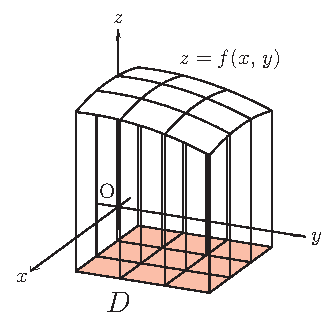
\includegraphics[width=6.5cm]{picture/juusekibun1.pdf} 
 \caption{マックのポテト}
\end{figure}

$D$を十分細かく分割すれば,
上に描いたマックのポテトのような立体の体積が$f(x, \, y)\:\mathrm{d}S$とみなすことができる.
これを領域$D$上すべての点で合計するのだから,
関数$z=f(x, \, y)$を領域$D$上で2重積分することで得られた値というのは
曲面$z=f(x, \, y)$と$D$の間の領域の体積を表していることになるというわけだ.
この場合でもこの値は負になることがある.
従って,この体積は符号付き体積とでも読んでおくべき量である.
ほとんど1変数関数のときと変わらないのである.

変数が増えても考えることは同じである.3変数関数$f(x, \, y, \, z)$をある領域$V$上で積分したければ,
まず$x, \, y, \, z$の微分$\mathrm{d}x, \, \mathrm{d}y, \, \mathrm{d}z$を考え,
これと$f(x, \, y, \, z)$との積$f(x, \, y, \, z)\:\mathrm{d}x\mathrm{d}y\mathrm{d}z$を作り,
そしてこれを$V$上全域にわたって足し合わせるのである.この値は
$$
\iiint_{V} f(x, \, y, \, z) \: \mathrm{d}x\mathrm{d}y\mathrm{d}z
$$
と書くことができるだろう.やはり,$\mathrm{d}x\mathrm{d}y\mathrm{d}z$という量が微小な体積を表しているのだと解釈できる.
したがってこれを$\mathrm{d}V$と置き換えてみると,この積分は
$$
\int_{V} f(x, \, y, \, z) \: \mathrm{d}V
$$
と書き換えられることになるというわけだ.
しかし,関数$f(x, \, y, \, z)$のグラフというのは4次元空間に存在するものであるから,
この積分を図に描けと言われてもそれは無理である.
しかし,計算することくらいは可能であろう.
変数が増えてくると,もはや積分を面積や体積などといった概念で解釈するのは不可能となる.
そのときはとりあえず1変数関数や2変数関数の積分と同じようなものを表しているのだろうと思っておくしかない.

\subsection{重積分の正確な定義}
さっき述べた定義は重積分の定義というよりは,その具体的なイメージである.
これでは定義としてあやふやなので,正確な定義を述べておこう.
変数の数がいくつでも同じやり方で定義するので,3重積分について述べておく.

$xyz$空間の領域$V$で定義された3変数関数$f(x, \, y, \, z)$について考える.
$V$はある範囲に収まった領域(つまり有界閉領域)としておき,
$V$を含むような十分大きな直方体$R$を考える.
\begin{align*}
R = \Set{ (x, \, y, \, z) | a_1\leq x \leq a_2 , \, b_1 \leq y \leq b_2 , \, c_1 \leq z \leq c_2 }
\end{align*}
とでも書いておこう.
そして,$R$上で定義された関数$f^* (x, \, y,\, z)$を
\begin{empheq}[left={f^*(x, \, y, \, z)=\empheqlbrace}]{alignat*=2}
f(x, \, y, \, z)  \quad & \Big( (x, \, y, \, z) \in V \Big) \\
0 \hspace{1cm} & \Big( (x, \, y, \, z) \not\in V \Big)
\end{empheq}
と定める.もともと$V$上でしか定義されていなかった関数の定義域を拡大したのだ.
$V$はどんな変な形をした領域かわかったものではない.
そこで,$V$の代わりに扱いやすい直方体を考えるのである.

さて,直方体$R$を分割しよう.そのような分割を$\varDelta$とおく.
\begin{empheq}[left={\varDelta : }]{align*}
a_1 & = x_0 < x_1 < \cdots < x_l = a_2 \\
b_1 & = y_0 < y_1 < \cdots < y_m = b_2 \\
c_1 & = z_0 < z_1 < \cdots < z_n = c_2 
\end{empheq}
というように表せるだろう.この分割により,$R$は微小直方体$R_{ijk}$に分割される.
\begin{align*}
R_{ijk} = \Set{ (x, \, y, \, z) | x_{i-1}\leq x \leq x_i , \, y_{j-1} \leq y \leq y_j , \, 
z_{k-1} \leq z \leq z_k }
\end{align*}
となる.さて,この微小直方体から1点$\mathrm{P} _{ijk} (p_i, \, p_j, \, p_k)$を任意にとり,
さらに$\varDelta x_i=x_i-x_{i-1} , \, \varDelta y_j = y_j - y_{j-1}, \, \varDelta z_k = z_k-z_{k-1}$
とおき,次のようなRiemann和\index[nidx]{Riemann@Riemann(リーマン)}
を考える.
\begin{align*}
\sum_{i, \, j, \, k} f^* (p_i, \, p_j, \, p_k) \varDelta x_i \varDelta y_j \varDelta z_k
\end{align*}
$\sum$の下に$i, \, j, \, k$と書いているのは,
$i, \, j, \, k$としてありうるものすべての和をとってくれという意味である.
いちいち$\sum$を3つも書かなくて済むのでこの書き方は便利である.
もし$\sum$を省略せずに書くのであれば,
\begin{align*}
\sum_{i=1}^{l} \sum_{j=1}^{m} \sum_{k=1}^{n} f^* (p_i, \, p_j, \, p_k) \varDelta x_i \varDelta y_j \varDelta z_k
\end{align*}
と表されるだろう.$i, \, j, \, k$はそれぞれ独立に動くので,どの$\sum$を先に計算しようと結果は変わらない.
そういうわけでさっきのような略記法が使えることになるのだ.

さて,このRiemann和に対して,各分割の幅を限りなく小さくしたときの極限を考えたい.
それには,$l, \, m, \, n \to \infty$と考えるか,あるいは
各微小直方体の体対角線(同じ面上にない頂点同士を結んだ線分)の長さの最大値$\delta$
が限りなく0に近づくと考えても同じことである.
すなわち,次のような極限を考えるのである.
\begin{align*}
\lim_{\delta \to 0} \sum_{i, \, j, \, k} f^* (p_i, \, p_j, \, p_k) \varDelta x_i \varDelta y_j \varDelta z_k
\end{align*}
もしこの極限が$\varDelta$や$\mathrm{P}_{ijk}$のとり方に依存せず,
一定の値に確定するのであれば,
$f(x, \, y, \, z)$は領域$V$上で\emph{可積分}\index[widx]{かせきぶん@可積分}であるといって,
その極限値を
\begin{align*}
\iiint_V f(x, \, y, \, z) \, \mathrm{d}x \mathrm{d} y \mathrm{d} z
\end{align*}
と表し,関数$f(x, \, y, \, z)$の領域$V$における\textbf{3重積分}と呼ぶ.

$x, \, y, \, z$というのは仮に用意した変数であって,別のものを用いてもよい.
そこで,後に学ぶ位置ベクトルを連想して,
$x, \, y, \, z$をまとめて$\bm{r}$という1つのベクトルで代表させて,積分を
\begin{align*}
\iiint_V f(x, \, y, \, z) \, \mathrm{d}^3 \bm{r}
\end{align*}
というように表すこともある.3乗のような記号がくっついているのは3重積分をイメージしてのことである.
あるいは,$\bm{r}$ではなく$\bm{x}$というベクトルで代表させれば
\begin{align*}
\iiint_V f(x, \, y, \, z) \, \mathrm{d}^3 \bm{x}
\end{align*}
というように表せる.上付きの3を省略してしまって
\begin{align*}
\iiint_V f(x, \, y, \, z) \, \mathrm{d} \bm{x}
\end{align*}
というように表すこともある.
書き方が違うだけで全部同じ積分を表す.混乱しないように気を付けよう.



ちょっと長くて混乱したかもしれないが,積分というのは結局
\begin{enumerate}
\item 積分領域を分割して
\item 分割された各領域から代表となる点をとり
\item その点における関数値とそこの領域の体積をかけて
\item その量を領域全体にわたって足し合わせて(ここまででRiemann和)\index[nidx]{Riemann@Riemann(リーマン)}
\item 各分割幅を限りなく小さくするような極限を考える
\end{enumerate}
だけなのである.
変数が増えようが,積分領域が変わろうが,
積分する対象が変わろうが,これだけは変わらない.
\footnote{ただし,この考えがよくないとして,あらためて積分の理論を組み立てなおした積分もあって,
それはLebesgue\index[nidx]{Lebesgue@Lebesgue(ルベーグ)}
積分と呼ばれている.この場合はもちろんこの考え方は当てはまらない.}
\begin{itembox}[l]{検討}
さっきやった方法では,$R$のうち,$V$の外側では値が0になるような関数$f^*(x, \, y, \, z)$を考えた.
これは,直方体$R$の$V$の外側の部分で積分値に変化がないようにするためである.

さて,``連続関数は可積分である''というのは有名な事実であるが,
元の関数$f(x, \, y, \, z)$が連続関数であっても,$f^*(x, \, y, \, z)$は$V$の境界線のところで
不連続になってしまうことがある.
このことは,可積分性に影響を与えることはあるだろうか?
\end{itembox}

\subsection{重積分の計算方法}
重積分の具体的なイメージは湧いただろうか? しかし,
イメージができたところで重積分が実際に計算できるかと言われたら話は別である.

ここでは領域$D$を
\begin{align*}
D= \Set{ (x, \, y) | 0 \leq x \leq y , \, 0 \leq y \leq 1}
\end{align*}
として,$D$上で関数$z = x + y$を積分してみる.
\begin{align*}
\iint_{D} z \, \mathrm{d}x \mathrm{d}y & = \iint_{D} (x+y) \, \mathrm{d}x \mathrm{d}y \\
& = \int_0^1 \left( \int_0^y (x+y) \, \mathrm{d}x \right) \mathrm{d}y \\
& = \int_0^1 \left[ \frac{1}{2} x^2 + xy \right]_0^y \mathrm{d}y \\
& = \int_0^1 \frac{3}{2} y^2 \, \mathrm{d}y \\
& = \left[ \frac{1}{2} y^3 \right]_0^1 = \frac{1}{2}
\end{align*}
普通に計算したように見えて,実はとても巧妙な技巧を使ってやっている.
いわゆる\emph{累次積分}\index[widx]{るいじせきぶん@累次積分}と呼ばれる手法である.
累次積分の真価は1行目から3行目あたりのところの式変形である.
あたかも$x$と$y$がまったく無関係に独立に変化しているかのように扱われているではないか!

実は,このような式変形ができるためには条件があって,
それは,積分領域を表す変数の変域のうちどれかが他の変数を含まない閉区間でなければならないというものである.
さっきの例では$x$の範囲は$0 \leq x \leq y$と,$y$を含んでいた.しかし,$y$の変域は$0 \leq y \leq 1$と,
$x$をまったく含んでいない.累次積分はこういう場合に使える技法である.
ただ単純に1変数関数での積分を2回やるだけである.
とはいえ,この非常に便利な技法が使えることをきちんと証明しようとすると,
やっぱり$\varepsilon - \delta$論法が必要になってくる.

きちんとまとめておくと,関数$f(x, \, y)$と領域$D$について,もし積分領域$D$が
\begin{align*}
D = \Set{ (x, \, y) | a \leq x \leq b , \, g(x) \leq y \leq h(x) }
\end{align*}
という形式で書けたとするならば,
\begin{align}
\iint_D f(x, \, y) \, \mathrm{d} x \mathrm{d} y
= \int_a^b \left( \int_{g(x)}^{h(x)} f(x, \, y) \, \mathrm{d} y \right) \mathrm{d}x 
\label{eq:ruijisekibuny}
\end{align}
と計算できる.この場合,$y$で積分するときには$x$はさも定数であるかのようにみなす.
偏微分のときと同じようなイメージである.
$x$で積分するときには$y$はすでに式中からなくなっており,
ただの定積分として計算できる.
なお,式(\ref{eq:ruijisekibuny})の右辺の積分を
\begin{align*}
\int_a^b \mathrm{d}x  \int_{g(x)}^{h(x)} f(x, \, y) \, \mathrm{d} y 
\end{align*}
と書き表すことがある.書き方が違ってもそれは式(\ref{eq:ruijisekibuny})
同じ積分を表している.単に書き方の問題である.

同じように領域$D$が
\begin{align*}
D = \Set{ (x, \, y) | g(y) \leq x \leq h(y) , \, a \leq y \leq b }
\end{align*}
という形式で書けたとするならば,
\begin{align}
\iint_D f(x, \, y) \, \mathrm{d} x \mathrm{d} y
= \int_a^b \left( \int_{g(y)}^{h(y)} f(x, \, y) \, \mathrm{d} x \right) \mathrm{d}y
\label{eq:ruijisekibunx}
\end{align}
と計算できることになる.
例によって,この式の右辺の積分は
\begin{align*}
\int_a^b \mathrm{d}y  \int_{g(y)}^{h(y)} f(x, \, y) \, \mathrm{d} x 
\end{align*}
と書かれることがある.
\begin{itembox}[l]{課題}
$xy$平面上での領域$D$を
\begin{align*}
D= \Set{ (x, \, y) | 0\leq y\leq 1-x , \, 0 \leq x \leq 1 }
\end{align*}
として,2重積分
\begin{align*}
\iint_{D} (x^2+y^2) \: \mathrm{d}x \mathrm{d}y
\end{align*}
を求めよ.

また,$xy$平面上の領域$D$を
\begin{align*}
D = \Set{ (x, \, y) | 0 \leq y \leq 1 , \, y \leq x \leq 1 }
\end{align*}
としたとき,2重積分
\begin{align*}
\iint_D \exp \left( \frac{y}{x} \right) \, \mathrm{d}x \mathrm{d}y
\end{align*}
を求めよ.(ヒント:$D$を図示してみよ)
\end{itembox}

\subsection{重積分の変数変換}
1変数関数の積分において,計算を進めるための技法として,置換積分法というのがあった.

$x$の関数$f(x)$があり,変数$x$が別の変数$t$の関数であり,$x=g(t)$と表せたとする.
$x$の微分$\mathrm{d}x$が
\begin{align*}
\mathrm{d}x = \frac{ \mathrm{d} x}{\mathrm{d} t } \mathrm{d} t 
\end{align*}
と表せることを利用して,$g(\alpha) = a, \, g(\beta) = b$となったとするとき
\begin{align}
\int_a^b f(x) \, \mathrm{d} x = \int_{\alpha}^{\beta} f(g(t))
\frac{ \mathrm{d} x}{\mathrm{d} t } \mathrm{d} t 
\label{eq:tikansekibun}
\end{align}
と計算するのであった.
この技法を重積分にも取り入れたい.
しかし,これは簡単そうで意外と面倒な事柄がたくさんあるのである.
なお,ここからの内容は先に第\ref{vecterop}章を読んでから取り組むことを推奨する.

\subsubsection{ヤコビ行列の登場}
話を簡単にするため,ここからは2重積分について考える.

$x, \, y$の2変数関数$f(x, \, y)$があり,変数$x, \, y$は別の変数$u, \, v$によって
$x=\varphi (u, \, v), \, y=\psi (u, \, v)$と表されていたとする.
ただし,各$(u, \, v)$と$(x, \, y)$が1対1に対応しているとしよう.
$x, \, y$の全微分はそれぞれ
\begin{align*}
\mathrm{d} x = \frac{\partial x}{\partial u} \mathrm{d}u + \frac{\partial x}{\partial v} \mathrm{d}v \\
\mathrm{d} y = \frac{\partial y}{\partial u} \mathrm{d}u + \frac{\partial y}{\partial v} \mathrm{d}v
\end{align*}
となるのだったから,
\begin{align*}
\mathrm{d}x \mathrm{d}y & = \left( 
\frac{\partial x}{\partial u} \mathrm{d}u + \frac{\partial x}{\partial v} \mathrm{d}v \right) 
\left( \frac{\partial y}{\partial u} \mathrm{d}u + \frac{\partial y}{\partial v} \mathrm{d}v \right) \\
& = \frac{\partial x}{\partial u} \frac{\partial y}{\partial u} (\mathrm{d}u)^2
+ \left( \frac{\partial x}{\partial u}\frac{\partial y}{\partial v} + 
\frac{\partial x}{\partial v}\frac{\partial y}{\partial u} \right) \mathrm{d}u \mathrm{d}v +
\frac{\partial x}{\partial v}\frac{\partial y}{\partial v} (\mathrm{d}v)^2
\end{align*}
と計算できそうだが,残念ながらこれは間違いである.
というのも,左辺は$x, \, y$を基準とした座標系,すなわち直交直線座標系で測ったときの
微小面積である.これを$u, \, v$を基準とした座標系
で測ったときには単純に積をとればいいというわけにはいかないのだ.
詳しいことは述べないので自分で考えてもらいたい.

ではどうすればいいかというと,全微分の式を行列形式で書き表してやって,
\begin{align}
\left[
\begin{array}{c}
\mathrm{d} x \\
\mathrm{d} y
\end{array}
\right]
= \left[
\renewcommand{\arraystretch}{2}
\begin{array}{cc}
\dfrac{ \partial x}{\partial u} & \dfrac{ \partial x}{\partial v} \\
\dfrac{ \partial y}{\partial u} & \dfrac{ \partial y}{\partial v} \\
\end{array}
\renewcommand{\arraystretch}{1}
\right]
\left[
\begin{array}{c}
\mathrm{d}u \\
\mathrm{d} v
\end{array}
\right]
\label{eq:jacobima}
\end{align}
としてみる.式(\ref{eq:jacobima})中に出てきた行列
\begin{align}
J = \left[
\renewcommand{\arraystretch}{2}
\begin{array}{cc}
\dfrac{ \partial x}{\partial u} & \dfrac{ \partial x}{\partial v} \\
\dfrac{ \partial y}{\partial u} & \dfrac{ \partial y}{\partial v} \\
\end{array}
\renewcommand{\arraystretch}{1}
\right]
\label{eq:jacobimatrix}
\end{align}
を座標変換$(u, \, v) \mapsto (x, \, y)$
\footnote{記号「$\mapsto$」は変換によって
$(u, \, v)$が$(x, \, y)$に対応することを指し示すために使われる記号である.}
の\emph{ヤコビ行列}\index[widx]{やこびあん@ヤコビ行列}と呼び,
その行列式
\begin{align}
\det J = \det \left[
\renewcommand{\arraystretch}{2}
\begin{array}{cc}
\dfrac{ \partial x}{\partial u} & \dfrac{ \partial x}{\partial v} \\
\dfrac{ \partial y}{\partial u} & \dfrac{ \partial y}{\partial v} \\
\end{array}
\renewcommand{\arraystretch}{1}
\right] = \left \lvert
\renewcommand{\arraystretch}{2}
\begin{array}{cc}
\dfrac{ \partial x}{\partial u} & \dfrac{ \partial x}{\partial v} \\
\dfrac{ \partial y}{\partial u} & \dfrac{ \partial y}{\partial v} \\
\end{array}
\renewcommand{\arraystretch}{1}
\right \rvert
\label{eq:jacobian}
\end{align}
を座標変換$(u, \, v) \mapsto (x, \, y)$の
\emph{ヤコビ行列式},\index[widx]{やこびぎょうれつしき@ヤコビ行列式|see{ヤコビアン}}
もしくは\emph{ヤコビアン}\index[widx]{やこびあん@ヤコビアン}と呼ぶ.
\footnote{名前のついた行列の行列式を表すとき,よく語尾を-ianと書き換えることが多い.
Jacobi\index[nidx]{Jacobi@Jacobi(ヤコビ)}行列の行列式ならJacobianという具合である.}

よく使うのはヤコビ行列よりもヤコビアンの方であり,ヤコビ行列が議論に出てくることはあまりない.
そういう事情からか,ヤコビ行列とヤコビアンがごっちゃになっていることがある.
文脈によってどちらを指しているのかきちんと見分ける癖をつけておこう.

また,ヤコビアンは次のような形で表されることもある.
\begin{align}
\frac{ \partial (x, \, y)}{ \partial (u, \, v) } = 
\left \lvert
\renewcommand{\arraystretch}{2}
\begin{array}{cc}
\dfrac{ \partial x}{\partial u} & \dfrac{ \partial x}{\partial v} \\
\dfrac{ \partial y}{\partial u} & \dfrac{ \partial y}{\partial v} \\
\end{array}
\renewcommand{\arraystretch}{1}
\right \rvert
\label{eq:jacobian2}
\end{align}
ヤコビアンは偏導関数を書き並べた行列の行列式であるから,
これを偏微分の拡張であるかのようにみなすイメージである.

さて,重積分の変数変換の文脈では,座標変換に対応したヤコビアンに対し,
\begin{align}
\mathrm{d} x \mathrm{d}y = \lvert \det J \rvert \, \mathrm{d} u \mathrm{d}v
\label{eq:jacobimenseki}
\end{align}
としてやるのが正しい.右辺の$\lvert \; \cdot \; \rvert$は絶対値を表す記号である.
行列式を表す記号と混同しないようにしてほしい.
なぜこれでうまくいくのだろう?

2つのベクトル
\begin{align*}
\left[
\renewcommand{\arraystretch}{2}
\begin{array}{c}
\dfrac{ \partial x}{\partial u} \\
\dfrac{ \partial y}{\partial u}
\end{array}
\right]
, \; \left[
\renewcommand{\arraystretch}{2}
\begin{array}{c}
\dfrac{ \partial x}{\partial v} \\
\dfrac{ \partial y}{\partial v}
\end{array}
\right]
\renewcommand{\arraystretch}{1}
\end{align*}
を見てみると,これは変数$u, \, v$が微小変化したときの$x, \, y$の変化の方向を表すベクトルである.
ヤコビ行列$J$を構成するベクトルは,変換後の座標系において$u , \, v$が微小変化したとき,
それが変換前の座標系ではどういう方向に変化するかを表していることになる.
線形代数学の知識によれば,ヤコビアン$\det J$はそれらのベクトルが張る平行四辺形の面積を表していることになる.
この``面積''というのはいわゆる符号付き面積のことだから,
絶対値を付けて正の値になるように調整していることになる.
1変数関数の置換積分のときには絶対値などは付けなかった.
これは,被積分関数が1変数関数であったため,変数の変化に向きがあったのだが,
重積分においては複数の変数が自由気ままに動き回り,変数の変化に向きなどないからである.

まとめよう.2変数関数$f(x, \, y)$を領域$D$上で積分するとき,
もし$x, \, y$が$x=\varphi (u, \, v) , \, y = \psi (u, \, v)$と表されていて,
かつ各$(u, \, v)$に対して$(x, \, y)$が1対1に対応しているとする.
点$(x, \, y)$が$D$上を動くときの点$(u, \, v)$が動く範囲を$D'$とすれば,
$D$上の各点$(x, \, y)$と$D'$上の点$(u, \, v)$が完全に1対1に対応することになる.
このとき,座標変換$(u, \, v) \mapsto (x, \, y)$のヤコビ行列を$J$として
\begin{align}
\iint_D f(x, \, y) \, \mathrm{d}x \mathrm{d} y 
= \iint_{D'} f( \varphi (u, \, v) , \, \psi (u, \, v) ) \, \lvert \det J \rvert \, \mathrm{d}u \mathrm{d}v
\label{eq:jusekibunhenkan}
\end{align}
という計算をしてやればよいということである.
式(\ref{eq:jacobian2})の表現方法を採用してみると
\begin{align}
\iint_D f(x, \, y) \, \mathrm{d}x \mathrm{d} y 
= \iint_{D'} f( \varphi (u, \, v) , \, \psi (u, \, v) ) 
\left \lvert \frac{ \partial (x, \, y) } { \partial (u, \, v) } \right \rvert \mathrm{d}u \mathrm{d}v
\label{eq:jusekibunhenkan2}
\end{align}
と表されることになる.こうしてみると,ヤコビアンを用いた重積分の変数変換が
1変数関数における置換積分法の拡張になっていることが一目瞭然である.

変数変換によって積分の式が余計にややこしくなったように見えるが,
右辺の方が簡単になるようにうまく座標変換を定義してやるのが腕の見せ所である.

今回は2重積分で話をしたが,変数の数が増えてもやることは同じである.
ただヤコビ行列の次数が増えていくだけである.

\subsubsection{具体例}
一般的な議論が済んだところで,ヤコビアンの力を実感するためにいくつか問題を解いてみよう.

$xy$平面上の領域$D$を
\begin{align*}
D = \Set{ (x, \, y) | 1 \leq  x+y \leq 2 , \, 1 \leq x-y \leq 3 }
\end{align*}
と定めたとき,関数$z=x^2-y^2$の$D$上での2重積分
を求めてみよう.
\begin{align*}
u = x + y \\
v = x - y 
\end{align*}
とおき,座標変換$(u, \, v) \mapsto (x, \, y)$を考える.
\begin{align*}
x = \frac{1}{2} u + \frac{1}{2} v \\
y = \frac{1}{2} u - \frac{1}{2} v
\end{align*}
と書けるので,
この座標変換のヤコビ行列$J$は
\begin{align*}
J = \left[
\renewcommand{\arraystretch}{2}
\begin{array}{cc}
\dfrac{ \partial x}{\partial u} & \dfrac{ \partial x}{\partial v} \\
\dfrac{ \partial y}{\partial u} & \dfrac{ \partial y}{\partial v} \\
\end{array}
\renewcommand{\arraystretch}{1}
\right] = \left[
\renewcommand{\arraystretch}{2}
\begin{array}{cc}
\dfrac{1}{2} & \dfrac{1}{2} \\
\dfrac{1}{2} & - \dfrac{1}{2}
\end{array}
\renewcommand{\arraystretch}{1}
\right]
\end{align*}
となり,この座標変換のヤコビアンは
\begin{align*}
\frac{ \partial ( x , \, y ) }{\partial (u, \, v ) } 
= \left \lvert
\renewcommand{\arraystretch}{2}
\begin{array}{cc}
\dfrac{1}{2} & \dfrac{1}{2} \\
\dfrac{1}{2} & - \dfrac{1}{2}
\end{array}
\renewcommand{\arraystretch}{1}
\right \rvert
= - \frac{1}{2}
\end{align*}
と計算できる.
\begin{align*}
D' = \Set{ (u , \, v) | 1 \leq u \leq 2 , \, 1 \leq v \leq 3 }
\end{align*}
とおけば,$D$上の各点$(x, \, y)$と$D'$上の各点$(u, \, v)$は1対1に対応し,
$z=x^2-y^2=(x+y)(x-y)=uv$と書けるので
\begin{align*}
\iint_D z \, \mathrm{d}x\mathrm{d}y 
& = \iint_{D'} uv \left \lvert - \frac{1}{2} \right \rvert \mathrm{d}u\mathrm{d}v \\
& = \int_1^3 \mathrm{d}v \int_1^2 \frac{1}{2} uv \, \mathrm{d} u \\
& = \int_1^3 \mathrm{d}v \left[ \frac{1}{4} u^2 v \right]_1^2 \\
& = \int_1^3 \frac{3}{4} v \, \mathrm{d}v \\
& = \left[ \frac{3}{8} v^2 \right]_1^3 \\
& = 3
\end{align*}
と計算できることになる.
このくらいの積分なら変数変換を使わずとも求めるのはさほど難易度は高くないのだが,
計算が煩雑になり,とても面倒である.

次に,$xyz$空間の領域$V$を
\begin{align*}
V = \Set{ (x, \, y, \, z ) | x^2 + y^2 + z^2 \leq R^2 }
\end{align*}
としたとき,関数$u=1$の$V$上での3重積分
を求めてみよう.
ただし$R$は正の定数とする.

点$(x, \, y, \, z)$を極座標系$(r, \, \theta, \, \varphi)$で表し,
\begin{align*}
x & = r \sin \theta \cos \varphi \\
y & = r \sin \theta \sin \varphi \\
z & = r \cos \theta 
\end{align*}
とおく.
この座標変換$(r, \, \theta , \, \varphi ) \mapsto (x, \, y, \, z)$のヤコビ行列$J$は
\begin{align*}
J = \left[ 
\renewcommand{\arraystretch}{2}
\begin{array}{ccc} 
\dfrac{ \partial x}{\partial r} & \dfrac{ \partial x}{\partial \theta} 
& \dfrac{ \partial x}{\partial \varphi} \\
\dfrac{ \partial y}{\partial r} & \dfrac{ \partial y}{\partial \theta} 
& \dfrac{ \partial y}{\partial \varphi} \\
\dfrac{ \partial z}{\partial r} & \dfrac{ \partial z}{\partial \theta} 
& \dfrac{ \partial z}{\partial \varphi} 
\end{array}
\renewcommand{\arraystretch}{1}
\right] = \left[
\begin{array}{ccc}
\sin \theta \cos \varphi & r \cos \theta \cos \varphi & - r \sin \theta \sin \varphi \\
\sin \theta \sin \varphi & r \cos \theta \sin \varphi & r \sin \theta \cos \varphi \\
\cos \theta & -r \sin \theta & 0
\end{array}
\right]
\end{align*}
となる.
よって,座標変換$(r, \, \theta , \, \varphi ) \mapsto (x, \, y, \, z)$のヤコビアンは,
余因子展開等を駆使して頑張って計算すると
\begin{align*}
\frac{ \partial (x, \, y, \, z) } { \partial (r, \, \theta , \, \varphi ) }
& = \left \lvert
\begin{array}{ccc}
\sin \theta \cos \varphi & r \cos \theta \cos \varphi & - r \sin \theta \sin \varphi \\
\sin \theta \sin \varphi & r \cos \theta \sin \varphi & r \sin \theta \cos \varphi \\
\cos \theta & -r \sin \theta & 0
\end{array}
\right \rvert \\
& = (-1)^{3+1} \cos \theta 
\left \lvert 
\begin{array}{cc}
r \cos \theta \cos \varphi & - r \sin \theta \sin \varphi \\
r \cos \theta \sin \varphi & r \sin \theta \cos \varphi 
\end{array}
\right \rvert \\
& \hspace{1cm} + (-1)^{3+2} ( - r \sin \theta ) 
\left \lvert 
\begin{array}{cc} 
\sin \theta \cos \varphi & - r \sin \theta \sin \varphi \\
\sin \theta \sin \varphi & r \sin \theta \cos \varphi 
\end{array}
\right \rvert \\
& = r^2 \cos \theta ( \sin \theta \cos \theta \cos ^2 \varphi 
+ \sin \theta \cos \theta \sin^2 \varphi ) \\ 
& \hspace{2cm} + r^2 \sin^3 \theta ( \cos ^2 \varphi + \sin ^2 \varphi ) \\
& = r^2 \sin \theta \cos ^2 \theta + r^2 \sin ^3 \theta \\
& = r^2 \sin \theta  
\end{align*}
となる.計算過程は面倒だが,結果はきれいな式となった.一生に一度は手を動かして計算しておこう.
その後は結果を暗記しておけばよい.

さて,
\begin{align*}
E = \Set{ (r, \, \theta , \, \varphi) 
| 0 \leq r \leq R , \, 0 \leq \theta \leq \pi , \, 0 \leq \varphi \leq 2 \pi }
\end{align*}
とおけば,$V$上の点$(x, \, y, \, z)$と$E$上の点$(r, \, \theta , \, \varphi)$
は1対1には対応しない.
しかし,1対1対応が崩れるような点は``ごくわずか''であり,
実はこのような場合でも変数変換は問題なく行えることが知られている.
このあたりの繊細な議論は本書の求めるものではないので考えないことにして,
さっさと積分を求めてしまおう.
\begin{align*}
\iiint_V 1 \, \mathrm{d} x \mathrm{d} y \mathrm{d} z 
& = \iiint_E \lvert r^2 \sin \theta \rvert 
\, \mathrm{d} r \mathrm{d} \theta \mathrm{d} \varphi \\
& = \int_0^{2\pi} \mathrm{d} \varphi \int_0^{\pi} \mathrm{d} \theta
\int_0^R r^2 \sin \theta \, \mathrm{d}r \\
& = \int_0^{2\pi} \mathrm{d} \varphi \int_0^{\pi} \mathrm{d} \theta
\left[ \frac{1}{3} r^3 \sin \theta \right]_0^R \\
& = \int_0^{2\pi} \mathrm{d} \varphi 
\int_0^{\pi} \frac{R^3}{3} \sin \theta \, \mathrm{d} \theta \\
& = \int_0^{2\pi} \mathrm{d} \varphi 
\left[ - \frac{R^3}{3} \cos \theta \right]_0^{\pi} \\
& = \int_0^{2\pi} \frac{2}{3} R^3 \, \mathrm{d} \varphi \\
& = \left[ \frac{2}{3} R^3 \varphi \right]_0^{2\pi} \\
& = \frac{4}{3} \pi R^3
\end{align*}
と,長らく慣れ親しんできた球の体積の公式が求められたことになる.

3次元の極座標変換におけるヤコビアンは$r^2 \sin \theta$であった.
2次元の極座標変換
\begin{align*}
x = r \cos \theta \\
y = r \sin \theta
\end{align*}
においてはヤコビアンは$r$となる.
計算は簡単なのでぜひともやっておき,結果を頭に叩き込んでおいてほしい.

\section{\textrm{Dirac}の$\delta$関数}
物理では,モノの位置を点で表現することがある.
質点や点電荷などがいい例である.
これらの概念は非常に便利である反面,
その密度を扱うときにちょっと困ったことが起こる.

とりあえず点電荷で考えてみよう.話を簡単にするために,1次元で考えてみる.
位置$a$に電荷量$q$の点電荷があるとする.
この点電荷の電荷密度を$\rho(x)$とおくと,
\begin{align}
q = \int_{- \infty}^{\infty} \rho ( x ) \, \mathrm{d} x 
\label{eq:denkamitudo}
\end{align}
が成り立っているはずである.
今回は積分範囲を$x$軸全体にしたが,点$a$さえ含まれていればどんな積分区間でも構わない.

ここからが問題である.
電荷は位置$a$にしか存在しないのだから,そこ以外の電荷密度はすべて0になっているはずで,
\begin{align*}
\rho ( x) = 0 \quad (\text{ただし$x \neq a$})
\end{align*}
が成り立つ.では$\rho (a)$はいくつだろう? $\rho (a) = q$とでもしておけばよさそうな気がする.
しかしこれでは式(\ref{eq:denkamitudo})を成り立たせることはできない.
それどころか$\rho(a)$をどんな値に定めようが無駄である.
いくら積分区間に点$a$が含まれていようとも,
区間を分割したときの幅が微小であるために1点だけで正で有限の値を持ったとしても
それが積分値に影響を与えないからだ.
つまり,式(\ref{eq:denkamitudo})をみたし,
かつ点$a$以外ではその値が0になるような関数は存在しないことになる.
これは困る.点電荷や質点は非常によく使う概念であるのにその密度がわからないというのだ!

\subsection{\textrm{Dirac}の解決策}
上記のような問題を解決するために,
物理学者Dirac\index[nidx]{Dirac@Dirac(ディラック)}
は次のような性質をみたす``関数''$\delta (x)$を編み出した.
\footnote{これは$\delta$関数の正確な出自とは違う.
Dirac自身は量子力学での問題を解決するのに$\delta$関数を利用した.}
\begin{itembox}[l]{定義}
任意の連続関数$f(x)$に対して
\begin{align}
\int_{-\infty}^{\infty} f(x) \, \delta (x) \, \mathrm{d}x = f(0)
\label{eq:deltadisdef}
\end{align}
をみたす``関数''$\delta(x)$を\textbf{Diracの$\delta$関数},
\index[widx]{でるたかんすう@$\delta$関数}
もしくは単に\textbf{$\delta$関数}と呼ぶ.
\end{itembox}
この``関数''を使えば,点$a$に存在する点電荷$q$の電荷密度は
\begin{align}
\rho (x) = q \, \delta ( x-a )
\label{eq:denkamitudodelta}
\end{align}
と求めることができる.
この$\rho(x)$が式(\ref{eq:denkamitudo})をみたすことは
置換積分法によって簡単に示すことができる.

また,$\delta$関数は次のような性質を持っている.
\begin{align}
\delta ( x) = \left \{
\begin{aligned} 
0 \hspace{4.2mm} & (x \neq 0) \\
\infty \quad & (x = 0)
\end{aligned}
\right.
\label{eq:deltainfty}
\end{align}
$\delta(0)$の値が有限の値では目的の性質が得られなかったので,
とりあえず$\infty$ということにしてある.この時点で怪しい香りがしてくる.
こんなものは性質とは言わない.$\delta$関数は積分して初めて意味を持つ.
こんな``関数''を関数として認めてしまっていいだろうか? ``編み出した''というのがどうもうさんくさい.
ずっと``関数''と表記していたのはこのためである.
ないものをあるとかたくなに言い張っているだけにしか見えない.
そんなうさんくさい概念を議論に持ち込んでいいものだろうか? この問題は多くの数学者,
物理学者を悩ませた.
$\delta$関数は物理学の役に立つし,必要不可欠なものである.
しかしその実態は何なのか? どう定義したらいいのか? ところが,それが解決されるのは案外早く,
わずか10年あまり後のことであった.
$\delta$関数などというわけのわからない概念を
関数の概念を拡張することによって定式化してみせたのである.
そのように拡張された関数のことを\emph{超関数}と呼ぶ.
通常の関数は英語ではfunctionというが,
超関数は英語ではdistributionということが多い.
しかし,超関数の定式化のやり方はいろいろあって,
その手法によっては違った呼ばれ方をされることもある.
超関数の詳しい定義は本書では取り上げることはしないが,
とりあえず$\delta$関数は数学的に定式化されたものであり,
決してよくわからない怪しい概念ではないということを理解しておいてほしい.
初学者向けに$\delta$関数のわけのわからなさを強調して話されることがよくあるが,
それはあくまで$\delta$関数が通常の意味での関数ではないということを伝えたいだけなのである.

\subsection{$\delta$関数の初等関数による近似}
いくら$\delta$関数が数学的に定式化されているとはいっても,
つかみどころのない不思議な関数であることには違いない.
そういうわけで,$\delta$関数をよく知っている関数の極限として考えるという方法がある.
たくさんあるが,その中でもよく見るものをピックアップしておこう.
\begin{align}
\phi_n (x) & = \left \{
\begin{aligned}
& \, n \quad & \left( \lvert x \rvert \leq \frac{1}{2n} \right) \\
& \, 0 \quad & \left( \lvert x \rvert > \frac{1}{2n} \right) 
\end{aligned}
\right. \\
\phi_n(x) & = \frac{ \sin nx}{\pi x} \\
\phi_n(x) & = \sqrt{ \frac{ n}{\pi}} \exp ( - nx^2)
\end{align}
これらの関数の$n \to \infty$としたときの極限として$\delta$関数を考えるのである.
これらの関数は$- \infty < x < \infty$の範囲で積分したときに常にその値が1になっているし,
\footnote{さらっと言っているがこれを厳密に証明するのは案外難しかったりする.}
なおかつ$x \neq 0$の範囲では$n \to \infty$としたときにその関数値が0に収束し,
$x = 0$のところでは$\infty$に発散する.
まさに$\delta$関数と同じような性質を持っているのである.
$n$をかなり大きめの有限の値にしておいて,$\delta$関数の代わりに
これらの関数を用いれば,完璧にではないにせよ
$\delta$関数のような関数を扱えることになる.
よく知っている初等関数の範囲で扱えるのが利点である.

\subsection{$\delta$関数の\textrm{Fourier}積分表示}
$\delta$関数のちょっと特殊な表現として,
次のようなものがある.
\begin{align}
\delta ( x ) = \frac{1}{2\pi} \int_{-\infty}^{\infty} \exp ( ikx) \, \mathrm{d}k
\label{eq:deltafourier}
\end{align}
なぜこの表現が特別視されているかというと,
この形が本書でカットしたFourier\index[nidx]{Fourier@Fourier(フーリエ)}
変換に深く結びついているからである.

なお,積分区間を有限にしたものであれば積分を実際に求めることができて,
\begin{align*}
\frac{1}{2\pi} \int_{-n}^{n} \exp ( ikx) \, \mathrm{d}k 
& = \frac{1}{2 \pi} \left[ \frac{1}{ix} \exp ( ikx) \right]_{-n}^n \\
& = \frac{1}{2 \pi ix} ( \exp ( inx ) - \exp( - inx) ) \\
& = \frac{ \sin nx} { \pi x}
\end{align*}
となる.Eulerの公式を思い出してほしい.
この式は先ほど説明した近似表現の1つである.
この式で$n \to \infty$としてやれば$\delta$関数が得られるのであった.
しかし,ここで重要なのは積分の形で書かれていることである.
Fourier変換を学んでみればそのあたりははっきりとわかるだろう.
そういうわけで,式(\ref{eq:deltafourier})は$\delta$関数の
\textbf{Fourier積分表示}と呼ばれている. 
\index[widx]{でるたかんすう@$\delta$関数!のふーりえせきぶんひょうじ@---のFourier積分表示}

\subsection{3次元での$\delta$関数}
先ほどやったのは1次元での$\delta$関数である.
しかし実際に点電荷の電荷密度などで利用するためには3次元でなくてはならない.
それはそんなに難しい話ではない.

点$( a, \, b, \, c)$に点電荷$q$が存在していることを表すには,
その電荷密度$\rho( x, \, y, \, z)$を$\delta$関数を使って次のように
表してやればいい.
\begin{align}
\rho ( x, \, y, \, z ) = q \, \delta( x -a ) \, \delta ( y-b) \, \delta( z-c)
\label{eq:deltamitudo3d}
\end{align}
このようにしてやれば,領域$V$が点$( a, \, b, \, c)$を含むとき
\begin{align}
\int_V \rho(x, \, y, \, z) \, \mathrm{d} V = q
\label{eq:delta3d}
\end{align}
は問題なく成り立つし,点$(a, \, b, \, c)$以外のところでは$\rho( x, \, y, \, z)=0$
が常に成り立っている.しかし,$x=a$で$y \neq b$などといった場合に少し困るが,
この際そういう細かいことは気にしないことにする.

また,いちいち$\delta$関数を3つも書くのは面倒なので,
\begin{align*}
 \delta ( \bm{r} ) , \, \delta ^{(3)} ( \bm{r})
 \end{align*}
 などと略記されることがある.書きたいことの意味はわかるだろう.
 この記法に従えば,位置$\bm{a}$にある点電荷$q$の電荷密度$\rho(\bm{r})$は
 \begin{align}
 \rho(\bm{r} ) = q \, \delta( \bm{r} - \bm{a} ) = q \, \delta^{(3) } ( \bm{r} - \bm{a})
 \label{eq:ryakkidelta}
 \end{align}
 と表せる.やっぱり表記は簡便な方がいい.
 
 $\delta$関数はもっとたくさんの面白い性質を秘めているのだが,
 そのあたりは類書に譲ることにしよう.
 物理学を学んでいればいずれまた遭遇するだろう. % 重積分
\chapter{ベクトルと座標系}\label{vecterop}
いままでやってきたのは実数に対して実数を返すような関数に関する微分積分学であった.
いまからやるのは,実数に対してベクトルを返したり,ベクトルに対して実数を返す,
もしくはベクトルに対してベクトルを返すような関数に関する微分積分学である.
何やら難しそうに思えるが実はそうでもない.実数のときの微分積分学の考え方がほぼそのまま使えるのだ.
これは,ベクトルの表し方を考えてみればすぐにわかる.早速やってみようといいたいところだが,
まずはベクトルとは何かを考えてみよう.
\section{ベクトルとその表現方法}
\subsection{ベクトルとは何か}
\emph{ベクトル量}\index[widx]{べくとる@ベクトル}
というのは,向きと大きさを持つ量のことだった.
対して,大きさのみを持つ量を\emph{スカラー量}\index[widx]{すからー@スカラー}
というのだった.
スカラー量を表したいときには,その大きさを表す実数を使えばよい.スカラー量とは実数である...という風に表現したくなるのだが,
現実はもう少し複雑である.正確な定義を述べるのはやや面倒なのでこのあたりで逃げておこう.
ただ,実数は大きさしか持たないからスカラー量とみなしていいだろう.

ベクトルとは向きと大きさを持つ量である...とさっき述べたのだが,実はこれもあまり正確な表現ではない.
さきほど実数は大きさしか持たないという話をした.実数を数直線上に図示してみれば,ただの点であり,方向性などない.
しかし,こうは考えられないだろうか? 方向性を持たないただの点であっても,原点とその点を結べば線分ができあがる.
この線分は原点からその実数に対応する点への向きを持つと考える.
いわゆる\emph{有向線分}\index[widx]{ゆうこうせんぶん@有向線分}
というやつである.
そして,実数というのは実はこの有向線分を表していたのだと考える.
いままで点だと思い込んでいたのはこの有向線分の終点だけを眺めて点だと言い張っていたにすぎないというように考えるのだ.
このように考えてみると,実数というものがあたかもベクトルであるかのように考えることができる.
だが,実数はスカラー量であるという主張にも一定の説得力がある.
いったいどっちなのだというのだろうか? ベクトル量でもありスカラー量でもある.
そんな量が存在するとでもいうのだろうか? この疑問は探求心のある読者のために大事に取っておくことにしよう.
とりあえずいまは,ベクトル量とは向きと大きさを持つ量であるというように認識しておくことにする.

\subsection{ベクトルの表記}
ベクトルは向きと大きさを持つのだった.
そんなものをいったいどうやって表したらいいだろうか? 高校まではおそらく矢印で表していたはずだ.
ベクトルの向きを矢印で,そしてベクトルの大きさを矢印の長さで表すのである.
これはベクトルを図示する方法である.記号で表したいときは,スカラー量と区別するために文字の上に矢印を乗せて
$\vec{a}$などというように表すのだった.これは``$a$ベクトル''や``ベクトル$a$''と読む.前者の読み方を使っている人が多い気がする.
この表記法は実に合理的である.
矢印で表されたベクトルを見れば,その向きと大きさがすぐにわかる.
$\vec{a}$という記号を見れば,これが向きと大きさを持ったベクトルだということが直感的にも理解できる.

だが,普通の専門書では$\to$を用いたベクトルの表記はしない.太字の文字を使って$\bm{a}$というように表記するのである.
なお,読み方はまったく同じで``$a$ベクトル''や``ベクトル$a$''と読む.
ちょっと見づらいが,慣れればなかなか美しいものである.なお,手書きで書くときには普通の文字に線を一本入れて二重文字で表記する.
線をどこに入れるかは好みでよい.あまりに見づらくなってしまうようなものだと困るが.人によって線の入れ方はさまざまである.
要は``この量はベクトル量ですよ''ということがわかればよいのである.
普通の文字が$a, \, b, \, c, \, \cdots$で,
ベクトル表記のものが$\bm{a}, \, \bm{b}, \, \bm{c}, \, \cdots$という具合である.
並べてみれば一目瞭然であるが,これを単独で見たときにきちんと判別しなければならない.
この記法を多用していれば自然と慣れてくるだろう.記号法というものは使って初めて身につくのである.

なぜ矢印ではなく太字を使うのだろうか? 少し考えてみよう.高校数学ではベクトルを何に使うかと言われれば,
図形問題を鮮やかに解くのに使われる.そう,まさにベクトルを矢印とまったく同じものとみなしているのである.
このとき使われるベクトルを\emph{幾何ベクトル}\index[widx]{べくとる@ベクトル!きか@幾何---}
という.ベクトルを一種の図形とみなしているのである.

しかし,これからやるのはそんなものではない.ベクトルを微分したり積分したりするのである.
つまり,ベクトルを関数だとみなすのである.
微分積分学は解析学の基礎的な部分を指す.
ベクトル解析という言葉はここからきている.
たしかに,計算した結果を幾何的に解釈することはあるが,あくまでオマケのようなものである.
このときに使われるベクトルは,もはや幾何ベクトルとはほど遠い.
そんな場合に矢印表記をしていては,むしろ誤解を招きかねない.
そこでベクトルを太字で表記する方法を用いるというわけだ.
その要請のもとは線形代数学にあるといってもいいだろう.
数学者はベクトルの概念を抽象化し,ベクトル空間なるものを考案した.
たしかにベースは幾何ベクトルである.しかし,中身は幾何ベクトルよりもはるかに広い概念を内包している.
そのような理論を組み立てるうえで矢印表記のベクトルは邪魔でしかない.
ベクトルを矢印以外の方法で表記するのはもはや必然である.
物理学でもこのあたりの話題を引っ張ってくることがよくある.量子力学なんかではしょっちゅうである.
\footnote{とはいうものの,量子力学ではブラ・ケット記法という
太字表記とはまた違ったベクトルの表記方法を採用していることが多い.}
分野や流儀によって表記や定義が違うというのはよくあることである.
違う分野や流儀に足を踏みいれるときにはまずそのあたりを確かめるとよい.

 \subsection{書体について}
 表記法をやったついでに書体についても触れておこう.
 普通,自然科学の分野では文字を表すときに\emph{イタリック体}と呼ばれる書体を使う.
 本書でも散々使っている書体である.$x, \, y, \, \varphi, \, A, \, B$などである.
イタリック体は,字がちょっと傾いているのが特徴である.手書きでは面倒なので傾けたりすることは普通しない.
 見返してみればほとんどの文字がイタリック体で書かれているはずである.
 
 しかし,それだけではないはずだ.
 傾いていないものがあるはずである.このような書体は\emph{ローマン体},もしくは
 \emph{立体}と呼ばれる.
 その書体は何を表すときに使われているだろうか? 特徴があるはずだ.
 使う場合はいろいろ考えられる.1つは点を表したいときである.$\triangle \mathrm{ABC}$や点$\mathrm{P}$などがある.
 $\triangle \mathrm{ABC}$というのは図形だが,
それを構成する$\mathrm{A}, \, \mathrm{B}, \, \mathrm{C}$は点である.
また,\emph{演算子}\index[widx]{えんざんし@演算子}なるものを表したいときにもローマン体が使われる.
演算子というのは単体で何かを表すというものではなく,何かの前にくっついてそれとペアで意味を持つものである.
正弦関数$\sin$や指数関数$\exp$,あとは微小量を表す$\mathrm{d}$など
だろうか.\footnote{$\mathrm{d}$に関してはイタリック体で書く流儀も多い.}
イタリック体で書いた通常の変数を表す文字と区別しなければ非常に面倒なことになるのがわかるだろう.
他にも,``いつも変わらない普遍的なモノ''や単位を表すのにもローマン体が使われることがある.
なんだかあいまいな気がするが,たとえばNapire数$\mathrm{e}$や虚数単位$\mathrm{i}$,
それに長さの単位である$[ \mathrm{cm} ]$や時間の単位である$[ \mathrm{s} ]$などである.
ベクトルを表すのにもローマン体が使われることがある.
太字とローマン体とを組み合わせて$\mathbf{x}$や$\mathbf{E}$というように表すのである.
他の本を読むときにはこの点には気を付けていただきたい.
ただし,見栄えが悪くなるので本書ではベクトルはイタリック体の太字で書かせてもらう.
もちろん,ここで書いたのはあくまでそういう傾向があるというだけであり,
そういう風に表記しなければならないと言っているわけではないということに気を付けてもらいたい.
本書でもNapire数$e$や虚数単位$i$などはイタリック体で表記している.
また,本書では原則として演算子と点,そして単位のみをローマン体とし,
他はイタリック体で表記することにする.
もちろんこのような表記法が世界共通というわけではない.
ただし,一度その流儀を採用すると決めたら,それを途中で変えるのは厳禁である.理由は言わなくてもわかるだろう.
無用な混乱は避けるべきである.

表記法に関してはこんなものだろうか.割とみんな好き勝手にやっているのが伝わってくれればそれでいい.

\subsection{数ベクトル空間}
ベクトルを微分したり積分したりしたければ,やっぱり関数が必要である.そのために,ベクトルの成分表示というものを考える.

3次元空間内にベクトル$\bm{a}$がある状況を考える.ベクトルには向きと大きさがある.ベクトルの始点を原点に固定してみよう.
ベクトルには向きと大きさがあるが,それ以外にはなにもない.
向きと大きさを変えないように動かしたところで(これを平行移動という)
やはり同じベクトルである.
ベクトルの始点を原点に固定したとき,その終点が点$(a_1, \, a_2, \, a_3)$であったとする.
いつでもベクトルの始点を原点に固定すると約束しておけば,終点の座標を決めるだけでベクトルを決めることができる.
つまり,終点の座標$(a_1, \,  a_2, \, a_3)$を書いておくだけでこのベクトルがどんなベクトルかわかるのである.
わざわざ矢印など書かなくとも,ただ数を3つ並べるだけでいいのだ.
この便利さを認め,点の座標と区別するために表記をちょっと変えて
\begin{align}
\bm{a} = \left[
 \begin{array}{c}
    a_1 \\
    a_2 \\
    a_3
 \end{array}
           \right]
 \label{eq:vec3d}
 \end{align}
 というように表記し,ベクトル$\bm{a}$の\emph{成分表示}
\index[widx]{べくとる@ベクトル!のせいぶんひょうじ@---の成分表示}と呼ぶことにしよう.人によっては
 $$
 \bm{a} = \left(
 \begin{array}{c}
    a_1 \\
    a_2 \\
    a_3
 \end{array}
           \right)
$$
と書いたり,数を横に並べて
$$
\bm{a} = (a_1, \, a_2, \, a_3)
$$
と書いたり,カンマを省略してしまって
$$
\bm{a} = (a_1 \ a_2 \ a_3)
$$
と書くこともある.数を1列に,つまり縦に並べて表記したベクトルを\emph{列ベクトル}
\index[widx]{べくとる@ベクトル!れつ@列---},
数を1行に,つまり横に並べて表記したベクトルを\emph{行ベクトル}
\index[widx]{べくとる@ベクトル!ぎょう@行---}という.
最近の線形代数学の流行に従って,本書では式番号を付けた列ベクトル表示を採用する.

ベクトル$\bm{a}$の列ベクトル表示
$$
\bm{a} = \left[
 \begin{array}{c}
    a_1 \\
    a_2 \\
    a_3
 \end{array}
           \right]
$$
において,$a_1$は終点の$x$座標に対応している.このことから,$a_1$をベクトル$\bm{a}$の
\emph{$x$成分}と呼ぶ.
$a_2$はベクトル$\bm{a}$の\emph{$y$成分},
$a_3$はベクトル$\bm{a}$の\emph{$z$成分}である.
このベクトル$\bm{a}$は空間上の1つの座標,つまり位置を指し示す.
このとき,このベクトルは\emph{位置ベクトル},\index[widx]{べくとる@ベクトル!いち@位置---}
もしくは単に\emph{位置}と呼ばれる.位置ベクトルを表すとき,よく記号$\bm{r}$が使われる.
位置$\bm{r}$が座標$(x, \, y, \, z)$を指し示すというのは
\begin{align}
\bm{r} = \left[
 \begin{array}{c}
  x \\
  y \\ 
  z 
 \end{array}
   \right]
\label{eq:itivec}
\end{align}
であるということだ.

さて,いま説明した列ベクトルは,あくまでベクトルの表現方法の1つである.
ベクトルを表すのに数を並べたものを使っているのだ.

ここで論理を逆転させて,数を並べたものそのものがベクトルだと考えてみる.いままでの幾何的イメージは並んだ数たちに
座標という概念を勝手に付け加えていたのだと解釈することにするのだ.
いまからベクトルとは``数が並んだものである''と考えることにしよう.
これを\emph{数ベクトル}\index[widx]{べくとる@ベクトル!すう@数---}と呼ぶ.
$x$成分,$y$成分,$z$成分という言葉は,
まだ我々が数ベクトルの各成分に座標という意味を勝手に付け加えていたころの名残である.
座標という縛りから解き放たれた今,この言葉はあまり使わない方がいいだろう.
そこで,$a_1$をベクトル$\bm{a}$の\emph{第$1$成分},
$a_2$をベクトル$\bm{a}$の\emph{第$2$成分},
$a_3$をベクトル$\bm{a}$の\emph{第$3$成分}と呼ぶことにしよう.
ただし,``次元''という言葉はそのまま使うことにする.
上に挙げたベクトルは3次の数ベクトルであるというわけだ.

こうして考えてみると,数を3つ並べたもののみを数ベクトルと呼ぶのには何ら必然性がない.
数1つだけだっていいし,2つ数を並べたり,4つや5つ数を並べたっていいだろう.
というわけで,数を$n$個並べたベクトルを考え,これを\emph{$n$次の数ベクトル}と呼ぶことにしよう.
$n$次の数ベクトル$\bm{a}$は$n$個の数$a_1, \, a_2, \, \cdots , \, a_n$を用いて
\begin{align}
\bm{a} = \left[
 \begin{array}{c}
   a_1 \\
   a_2 \\
   \vdots \\
   a_n 
 \end{array}
            \right]
\label{eq:vecnd}
\end{align}
と表せるというわけだ.上から$i$番目の数$a_i$をベクトル$\bm{a}$の\emph{第$i$成分}と呼ぶ.
3次元の場合の素直な拡張になっているのが見てわかるだろう.

また,各成分がすべて0であるようなベクトルを$\bm{0}$と表し,
これを\emph{\ruby{零}{れい}ベクトル}\index[widx]{べくとる@ベクトル!れい@零---}という.
\begin{align}
\bm{0} = \left[
 \begin{array}{c}
   0 \\
   0 \\
   \vdots \\
   0
  \end{array}
   \right]
\label{eq:reivec}
\end{align}
である.零ベクトルは大きさが0のベクトルであるのでその向きは考えない.
このことからもベクトルの定義が割とあいまいであることが感じ取れるだろう.
零ベクトルはあった方が何かと便利なので導入されるにすぎない.

また,零ベクトルは太字で$\bm{0}$であり,手書きのときには二重文字で書く.
普通の数としての零は太字でない0であり,手書きのときでももちろんそのまま書く.
間違えやすいので気を付けよう.きちっと書き分ける癖がついてしまえばなんてことはないのだが.
\section{ベクトルの演算}
\subsection{ベクトルの和,差,スカラー倍}
ベクトルを数が並んだものとして表したからにはそこに演算を導入したくなる.
ここではベクトルの和,差,スカラー倍の3つの演算を考えよう.
\subsubsection{ベクトルの和}
2つのベクトル
$$
\bm{a} = \left[
 \begin{array}{c}
   a_1 \\
   a_2 \\
   \vdots \\
   a_n 
 \end{array}
            \right]
\, , \; 
\bm{b} = \left[
 \begin{array}{c}
   b_1 \\
   b_2 \\
   \vdots \\
   b_n 
 \end{array}
            \right]
$$
について,その和$\bm{a}+\bm{b}$を
\begin{align}
\bm{a}+\bm{b} = \left[
 \begin{array}{c}
   a_1+b_1 \\
   a_2+b_2 \\
   \vdots \\
   a_n+b_n 
 \end{array}
\right]
\label{eqn:vecsum}
\end{align}
と定義する.直感的にも受け入れやすい定義である.
左辺の$+$は新しく定義したベクトルの和,右辺のカッコの中にある$+$は既知の数の和であることに注意しよう.
\subsubsection{ベクトルの差}
2つのベクトル
$$
\bm{a} = \left[
 \begin{array}{c}
   a_1 \\
   a_2 \\
   \vdots \\
   a_n 
 \end{array}
            \right]
\, , \; 
\bm{b} = \left[
 \begin{array}{c}
   b_1 \\
   b_2 \\
   \vdots \\
   b_n 
 \end{array}
            \right]
$$
について,その差$\bm{a}-\bm{b}$を
\begin{align}
\bm{a}-\bm{b} = \left[
 \begin{array}{c}
   a_1-b_1 \\
   a_2-b_2 \\
   \vdots \\
   a_n-b_n 
 \end{array}
\right]
\label{eqn:vecsa}
\end{align}
と定義する.こちらも何のひねりもない定義である.
これも左辺にある$-$は新しく定義したベクトルの差であり,右辺のカッコの中にある$-$は既知の数の差である.
\subsubsection{ベクトルのスカラー倍}
ベクトル
$$
\bm{a} = \left[
 \begin{array}{c}
   a_1 \\
   a_2 \\
   \vdots \\
   a_n 
 \end{array}
\right]
$$
とスカラー量$k$について,スカラー倍$k\bm{a}$を
\begin{align}
k\bm{a} = \left[
 \begin{array}{c}
   ka_1 \\
   ka_2 \\
   \vdots \\
   ka_n 
 \end{array}
\right]
\label{eq:vecsukara}
\end{align}
と定義する.スカラー$k$と書いたところは$k$がただの数であることを表している.
これも特に変わったところはないだろう.

とりあえずここで書くことは以上である.
幾何学的解釈は高校の教科書に散々書かれているだろうから省略させてもらうことにする.
\subsection{ベクトルの内積}
さっきまでやったのはベクトル同士の和,差,そしてベクトルのスカラー倍である.
ここでは,ベクトル同士の積について考えよう.
ただし,ベクトル同士の``積''は定義がちょっと特殊である.
そして,よく使われるのが2種類あり,
それぞれベクトルの内積,外積と呼ばれている.
まずは内積から片づけてしまおう.
\subsubsection{内積の定義}
2つのベクトル
$$
\bm{a} = \left[
 \begin{array}{c}
   a_1 \\
   a_2 \\
   \vdots \\
   a_n 
 \end{array}
            \right]
\,  ,  \;  
\bm{b} = \left[
 \begin{array}{c}
   b_1 \\
   b_2 \\
   \vdots \\
   b_n 
 \end{array}
            \right]
$$について,その\emph{内積}$\bm{a} \cdot \bm{b}$を
\index[widx]{べくとる@ベクトル!のないせき@---の内積}
\begin{align}
\bm{a} \cdot \bm{b} = a_1 b_1 + a_2 b_2 + \cdots + a_n b_n
\label{eq:naiseki}
\end{align}
と定義する.「$\cdot$」は普通に``ドット''と読めばよい.
内積はベクトルではなく$1$つの実数である.内積はベクトルとベクトルの積であるが,
結果は1つのスカラー量である.
内積を求めたければ同じ場所にある成分をかけて,その総和をとるのである.
覚えやすいだろう.ただし,左辺にある「$\cdot$」は重要である.これを書き忘れたら内積とは言わない.
ベクトルの積は2種類あるといった.内積を表す記号「$\cdot$」を書き忘れたら何が書いてあるのかよくわからなくなるだろう.
記号法のルールをしっかり守れるというのは自分が何をやっているのか正確に把握できているということなのだ.
このドットの存在から,
内積のことを\emph{ドット積}\index[widx]{べくとる@ベクトル!のどっとせき@---のドット積|see{内積}}
と呼ぶことがある.
ドット積といえば内積を表す「$\cdot$」を忘れることはないだろう.

\subsubsection{ベクトルのノルム}
内積の定義は式(\ref{eq:naiseki})の通りであるが,ここで,あるベクトルと自身との内積を考えてみる.
$$
\bm{a} = \left[
 \begin{array}{c}
  a_1 \\
  a_2 \\
  \vdots \\
  a_n
 \end{array}
 \right]
$$
とすれば,$\bm{a}$と$\bm{a}$との内積は
\begin{align*}
\bm{a} \cdot \bm{a} & =  a_1 a_1 + a_2 a_2 + \cdots + a_n a_n \\
& = a_1^2+a_2^2+\cdots+a_n^2
\end{align*}
となる.右辺が何を表しているかは$n=2$としてみればすぐにわかる.
$n=2$の場合は
$$
\bm{a} \cdot \bm{a} = a_1^2 + a_2^2
$$
となるが,これは$xy$平面上の原点と点$(a_1, \, a_2)$との距離の2乗である.
つまり,$\bm{a} \cdot \bm{a}$の正の平方根をとったものは距離を表すということだ.
$$
\sqrt{\bm{a}\cdot\bm{a}} = \sqrt{a_1^2 + a_2^2} 
$$
ということである.これを$n$次元に拡張してみれば
$$
\sqrt{\bm{a}\cdot\bm{a}} = \sqrt{a_1^2 + a_2^2+\cdots + a_n^2}
$$
という量を考えることができる.
この量は何かしらの``距離''を表していると推測できる.2次元のときと同じものを表しているだろうと勝手に思うのである.

さて,幾何ベクトルの考え方では,始点と終点の距離というのはベクトルを矢印とみなしたときの長さ,
すなわちベクトルの大きさを表しているのだった.
$n$次の数ベクトルに対しても同じ解釈をしてやろう.
$\sqrt{\bm{a}\cdot\bm{a}}$という量がベクトル$\bm{a}$の大きさを表すと考えるのである.
そこで,$\sqrt{\bm{a}\cdot\bm{a}}$をベクトルの\emph{大きさ},
\index[widx]{べくとる@ベクトル!のおおきさ@---の大きさ}
もしくは\emph{絶対値}\index[widx]{べくとる@ベクトル!のぜったいち@---の絶対値}
と呼ぶことにして,$\lvert \bm{a} \rvert$という記号で表そう.
\begin{align}
\lvert \bm{a} \rvert = \sqrt{\bm{a}\cdot\bm{a}}
\label{eq:vecabs}
\end{align}
である.これは幾何ベクトルのときのベクトルの大きさの定義の拡張になっている.

ただし,ベクトルを幾何ベクトルから完全に切り離して議論したいとき,
``ベクトルの大きさ''という呼び方や$\lvert \bm{a} \rvert$記法はむしろ誤解を招くことがある.
こういうことに用心深い数学者は,$\sqrt{\bm{a}\cdot\bm{a}}$をベクトル$\bm{a}$の絶対値や大きさでなく
\emph{ノルム}\index[widx]{べくとる@ベクトル!ののるむ@---のノルム}
と呼び,記号も変えて$\| \bm{a} \|$と書き表す.
\begin{align}
\| \bm{a} \| = \sqrt{\bm{a}\cdot\bm{a}}
\label{eq:norm}
\end{align}
と定義するのである.本書は物理数学の本なので,
記号は$\lvert \bm{a} \rvert$を採用し``ベクトルの絶対値''や``ベクトルの大きさ''
という用語も普通に使わせてもらう.

\subsubsection{内積の意味}
内積の定義は覚えやすい式であるが,どうも何を表しているかわかりにくい.とりあえず3次元で考えてみよう.

高校までは,ベクトルの内積を次のように定義していたはずだ.
\begin{itembox}[l]{定義}
2つのベクトル$\vec{a}$と$\vec{b}$のなす角を$\theta$として,$\vec{a}$と$\vec{b}$との内積$\vec{a} \cdot \vec{b}$を
\begin{align}
\vec{a} \cdot \vec{b} = \lvert \vec{a} \rvert \lvert \vec{b} \rvert \cos \theta
\label{eq:kikavecnaiseki}
\end{align}
と定義する.
\end{itembox}
ここに書いた$\lvert \vec{a} \rvert$や$\lvert \vec{b} \rvert$というのは幾何ベクトルの長さである.
ちょうど矢印の長さに対応している.
これは直感的に解釈しやすい.2つのベクトルが長いほど,また向きがそろっているほど内積の値は大きくなる.
我々はいま,3次元での数ベクトルの内積を
$$
\bm{a} \cdot \bm{b} = a_1 b_1 + a_2 b_2 + a_3 b_3
$$
と定義した.これらは同じものとなっているはずである.3次元空間において,式(\ref{eq:naiseki})
から式(\ref{eq:kikavecnaiseki})を導いてみよう.
それには$\cos \theta$を求めなくてはなるまい.余弦定理を用いればよい.
始点を原点$\mathrm{O}$として,$\bm{a}, \, \bm{b}$の終点をそれぞれ$\mathrm{A}, \, \mathrm{B}$とすれば,
$$
\overrightarrow{\mathrm{OA}}+\overrightarrow{\mathrm{AB}}=\overrightarrow{\mathrm{OB}}
$$
だから,
$$
\overrightarrow{\mathrm{AB}}=\overrightarrow{\mathrm{OB}} - \overrightarrow{\mathrm{OA}}
$$
よって
$$
\overrightarrow{\mathrm{AB}} = \bm{b} - \bm{a}
$$
が成り立つ.
$$
\bm{b} - \bm{a} = \left[
 \begin{array}{c}
  b_1 \\
  b_2 \\
  b_3 
  \end{array}
\right]
-
\left[
\begin{array}{c}
 a_1 \\
 a_2 \\ 
 a_3
 \end{array}
 \right]
 =
 \left[
 \begin{array}{c}
  b_1 - a_1 \\
  b_2 - a_2 \\
  b_3 - a_3
  \end{array}
 \right]
$$
となるので,$\angle \mathrm{AOB} = \theta$として$\triangle \mathrm{ABC}$において余弦定理を用いれば,
\begin{align*}
\lvert \overrightarrow{\mathrm{AB}} \rvert^2 = 
\lvert \overrightarrow{\mathrm{OA}} \rvert^ 2 + \lvert \overrightarrow{\mathrm{OB}} \rvert^ 2
-2 \lvert \overrightarrow{\mathrm{OA}} \rvert \lvert \overrightarrow{\mathrm{OB}} \rvert \cos \theta
\end{align*}
が成り立ち,式(\ref{eq:naiseki})と式(\ref{eq:vecabs})を用いてこれを計算すると,
\begin{align*}
\lvert \bm{a} \rvert \lvert \bm{b} \rvert \cos \theta = a_1 b_1 + a_2 b_2 + a_3 b_3
\end{align*}
が成り立っていることがわかる.(各自計算せよ)すなわち,
\begin{align}
\bm{a} \cdot \bm{b} =\lvert \bm{a} \rvert \lvert \bm{b} \rvert \cos \theta 
\label{eq:koukounaiseki}
\end{align}
が成り立っているということである.
いま,式(\ref{eq:naiseki})をベクトルの内積と定義として採用し,それを用いて式(\ref{eq:koukounaiseki})を導いた.
これはつまり,内積の2つの定義はどちらを採用しても構わないということだ.どちらもまったく同じ値を示すのである.
ただし,成分表示された内積の方が多次元へと拡張しやすいので本書は$\cos$を用いた定義ではなく成分表示の方を採用したのである.

さて,ここまでくると内積が何を表しているのかが見えてくる.
$$
\bm{a} \cdot \bm{b} = \lvert \bm{a} \rvert \lvert \bm{b} \rvert \cos \theta 
$$
のうちの$\lvert \bm{b} \rvert \cos \theta$という部分について考えてみよう.
これは,$\bm{b}$の$\bm{a}$方向の成分を表している.何を言っているかわからなければ,次の図を見てほしい.
\begin{figure}[h]
 \centering
 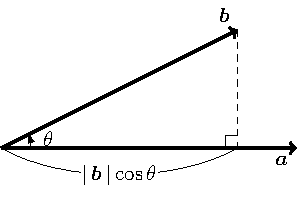
\includegraphics[width=6cm]{picture/vecter1.pdf}
 \caption{内積は何を表すか}
\end{figure}

$\lvert \bm{b} \rvert \cos \theta$というのは
$\bm{b}$が$\bm{a}$の方向にどれだけの長さを持っているかを表しているのである.
もちろん$\lvert \bm{a} \rvert \cos \theta$という部分を考えてもよい.
このとき,この量は$\bm{a}$が$\bm{b}$の方向にどれだけの長さを持っているかを表している.
いまは3次元空間でやってみたが,$n$次元空間でもそうなっていると思ってみよう.
$n$次元空間での角度や方向など意味不明だが,3次元空間でのイメージをそのまま持ってくるのである.
つまり,ベクトルの内積は
片方のベクトルがもう片方のベクトルの方向
にどれだけの長さを持っているかを表しているのである.
この解釈は今後もよく使うので覚えておいていただきたい.

この解釈から,
2つのベクトルが直交するための条件は,
そのベクトルの内積が0になることであるという重要な事実がわかる.
数学的にいえば$\theta = 90^\circ$のとき$\cos \theta = 0$になるということである.

ベクトルの内積に関してはこんなものである.演習を1つしてみようか.
\begin{itembox}[l]{問}
3次元空間において,2つのベクトル$\bm{a}, \, \bm{b}$の内積を,
$\bm{a}$と$\bm{b}$のなす角を$\theta$として
$$
\bm{a} \cdot  \bm{b} = \lvert \bm{a} \rvert \lvert \, \bm{b} \rvert \cos \theta
$$
と\.定\.義したとき,
$$
\bm{a} \cdot \bm{b} = a_1 b_1 +a_2 b_2 + a_3 b_3
$$
が成り立っていることを\.証\.明せよ.ただし
$$
\lvert \bm{a} \rvert = \sqrt{a_1^2 + a_2^2 + a_3^2} \ ,\ \lvert \bm{b} \rvert = \sqrt{b_1^2 + b_2^2 + b_3 ^2}
$$
である.
\end{itembox}
\subsection{単位ベクトルと標準基底}
ベクトルを使っていると,あるベクトルの向きだけを利用したいということがよくある.
たとえば,$\bm{r}$と同じ方向を向いていて,大きさ$\displaystyle \frac{1}{4 \pi \varepsilon_0} \frac{q}{r^2}$
のベクトルを考えたいなどである.こういうことはよくある.そのための手法は割と簡単なので知っておこう.

ベクトル$\bm{r}$の大きさを$r$と書く.これは物理ではよくやる書き方である.この$r$で$\bm{r}$を割ったものを考えれば,
その大きさは1になる.このベクトルは$\displaystyle \frac{\bm{r}}{r}$である.
そして,このベクトルの方向は,もちろん$\bm{r}$と同じ方向を向いている.
このベクトルに大きさである
$\displaystyle \frac{1}{4 \pi \varepsilon_0} \frac{q}{r^2}$をかけてやれば目的のベクトルが得られる.
これを$\bm{E}$と書けば,
$$
\bm{E} = \frac{1}{4 \pi \varepsilon_0} \frac{q}{r^2} \frac{\bm{r}}{r} 
$$
となるのである.\footnote{これは静電場である.}

このように,大きさが1のベクトルは何かと使いやすい.その向きだけを自由に使えるからである.
大きさが1のベクトルを\emph{単位ベクトル}\index[widx]{べくとる@ベクトル!たんい@単位---}
という.
大きさが1だから``単位''である.

さて,単位ベクトルのなかで,次のようなものを考えてみよう.
\begin{align}
\bm{e}_1 = \left[ 
 \begin{array}{c}
  1 \\
  0 \\
  0 \\
  \vdots \\
  0
 \end{array}
 \right]
  , \, 
 \bm{e}_2 = \left[ 
 \begin{array}{c}
  0 \\
  1 \\
  0 \\
  \vdots \\
  0
 \end{array}
 \right]
 \, , \, 
 \cdots 
 , \, 
 \bm{e}_n = \left[ 
 \begin{array}{c}
  0 \\
  0 \\
  0 \\
  \vdots \\
  1
 \end{array}
 \right]
 \label{eq:hyoujunnkitei}
\end{align}
これらはすべて単位ベクトルで,すべてのベクトルが互いに直交している.
この集団$\{ \, \bm{e}_1, \, \bm{e}_2, \, \cdots , \, \bm{e}_n \, \}$を
$n$次元数ベクトル空間の\emph{標準基底}
\index[widx]{きてい@基底!ひょうじゅん@標準---}と呼ぶ.
なぜか$ \{ \cdots \} $がついているが,ベクトルを集めてこれらをまとめて扱うとき,
こういう風にカッコでまとめるのが習わしである.
しかし集合を表すカッコとはまたちょっと違うのだそうだ.
なんだそれ? という感じである.
話を戻そう.$n$次元数ベクトル空間のすべてのベクトルはこれらの標準基底の組み合わせで表すことができる.
実際,任意のベクトル$\bm{a}$を成分表示して
$$
\bm{a} = \left[
 \begin{array}{c}
  a_1 \\
  a_2 \\
  \vdots \\
  a_n
 \end{array}
 \right]
$$
と書き表すとき,$\bm{a}$は
\begin{align}
\bm{a} = a_1 \bm{e}_1 + a_2 \bm{e}_2 + \cdots + a_n \bm{e}_n
\label{eq:veckiteihyougenn}
\end{align}
と書き表すことができる.この形式もよく使うので覚えておいてもらいたい.

また,3次元数ベクトル空間においては,標準基底を$\bm{e}_x, \, \bm{e}_y, \, \bm{e}_z$と表したり,
$\bm{i} , \, \bm{j}, \, \bm{k}$などと表したりすることがある.
力学なんかだとよく$\bm{i}, \, \bm{j}, \, \bm{k}$という表現を目にすることがあるだろう.
その本において記号がどういう意味で使われているのかはまちまちであるから,逐一確かめる癖をつけておこう.

ともかく,これで外積をやる準備が整った.とっとと片づけてしまおう.
\subsection{ベクトルの外積}
ベクトルの積は2種類あるといった.1つはさっきやった内積である.もう1つはこれからやる外積である.
内積はベクトル2つから1つの実数を作り出す演算であったが,外積はベクトル2つから新たなベクトルを1つ作り出す演算である.

また,内積は一般の$n$次元の数ベクトル空間で定義したが,外積に関しては3次元空間に限らせてもらう.
外積を一般の$n$次元の数ベクトル空間に拡張できないこともないのだが,
内積と違って話がかなり複雑になってしまうことが知られている.\footnote{超複素数なる理論を使うらしい.}
そんなことをしても物理学を学ぶ上であまりいいこともないので,とりあえず3次元空間で話をしよう.
\subsubsection{まずは定義から}
外積の定義は,内積のときと同じく幾何学的に定義する手法と成分表示で定義する手法との2種類あるのだが,
今回は幾何学的に定義する方でやってみよう.

2つのベクトル$\bm{a}, \, \bm{b}$について,その外積を$\bm{a} \times \bm{b}$と書く.
\index[widx]{べくとる@ベクトル!のがいせき@---の外積}
``$\times$''は``クロス''と読むのが一般的らしい.``$\bm{a} \times \bm{b}$''は``$\bm{a}$クロス$\bm{b}$''と読むのである.
このことから,ベクトルの外積は\emph{クロス積}
\index[widx]{べくとる@ベクトル!のくろすせき@---のクロス積}とも呼ばれる.
ただ,``$\times$''を普通に``かける''と呼んでしまう人も多い.


外積はベクトルである.ベクトルというからには向きと大きさがあるはずだ.
逆に,向きと大きさが決まればベクトルはただ1つに定まるといえる.
そこで,ベクトルの外積をその向きと大きさにわけて定義しよう.

外積$\bm{a} \times \bm{b}$の大きさは,$\bm{a}$と$\bm{b}$がなす角を$\theta$として
\begin{align}
\lvert \bm{a} \times \bm{b} \rvert = \lvert \bm{a} \rvert \lvert \bm{b} \rvert \sin \theta 
\label{eq:gaisekiookisa}
\end{align}
であると定義する.これは,$\bm{a}$と$\bm{b}$が張る平行四辺形の面積を表している.
\begin{figure}[h]
 \centering
 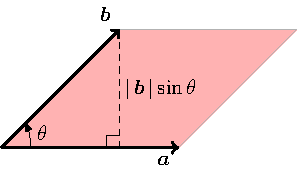
\includegraphics[width=5.5cm]{picture/vecter2.pdf}
 \caption{2つのベクトルが張る平行四辺形}
\end{figure}

図に赤色で示した領域が$\bm{a}$と$\bm{b}$が張る平行四辺形であり,
$\lvert \bm{a} \rvert$がその底辺,$\lvert \bm{b} \rvert \sin \theta$がその高さになっている.
内積のときは$\cos$を使ったのに対して外積の大きさは$\sin$である.
外積の大きさは2つのベクトルが直交している状態に近いほど大きくなるのである.
対して内積の値は2つのベクトルが平行である状態に近いほど値は大きくなり,直交しているときにはその値は0になるのだった.
結果がベクトルかスカラーかの違いはあるものの,内積と外積はなかなか対称的なものになっている.

次は向きである.外積$\bm{a} \times \bm{b}$の向きは$\bm{a}$から$\bm{b}$の向きに右ネジを回したとき,
そのネジが進む方向であると定義する.
\begin{figure}[h]
 \centering
 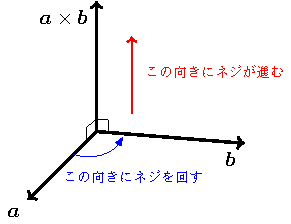
\includegraphics[width=6cm]{picture/vecter3.pdf}
 \caption{外積の向き}
\end{figure}

2つのベクトル$\bm{a}, \, \bm{b}$とその外積$\bm{a} \times \bm{b}$の向きの関係はこのようになっている.
``右ネジ''という言葉になじみがなければ自分の右手を見てほしい.親指以外の指をガッツポーズを緩めた感じに丸めてみる.
一種の渦のようなものが見えただろうか.指の根元から先に向かって渦が巻いているイメージである.
そして,そのときに親指が向いている方向がネジの進む方向になっている.``右手''だから``右ネジ''なのである.
親指以外の指をガッツポーズを緩めた感じに丸め,$\bm{a}$の方向を指の根元に,そして$\bm{b}$の方向に指の先を向けてほしい.
そして,そのとき親指が指し示す方向が外積$\bm{a} \times \bm{b}$の方向である.右ネジよりもこちらの方が覚えやすいかもしれない.
なによりいつでも再現できる.私は右ネジの覚え方より右手の覚え方の方が好きである.読者の方々はどうだろうか? 

ネジの回転面とネジの進む方向は明らかに直交している.つまり,
\begin{align}
\bm{a} \cdot ( \, \bm{a} \times \bm{b} \, ) = 0 \: , \:  \bm{b} \cdot ( \, \bm{a} \times \bm{b} \, ) =0 
\label{eq:naisekigaiseki}
\end{align}
という関係式が成り立っている.右辺の0はスカラー量である.
式中にあるカッコは重要である.左側では$\bm{a}$というベクトルと$\bm{a} \times \bm{b}$というベクトルの内積をとっている.
これを
\begin{align*}
\bm{a} \cdot \bm{a} \times \bm{b}
\end{align*}
のように書いてしまうようなことはしてはいけない.カッコはモノのかたまりを表すのである.
また,式(\ref{eq:naisekigaiseki})が成り立っていることは図を見てもらえれば納得できるはずだ.
直交する2つのベクトルの内積は0になるのだった.

そういえば,上の説明で$\bm{a} \times \bm{b}$と$\bm{b} \times \bm{a}$が異なったベクトルになるということはわかるだろうか? 
ネジを回す向きを逆にすればネジが進む方向も逆になる.
$\bm{a} \times \bm{b}$と$\bm{b} \times \bm{a}$とで向きは逆になる.しかし大きさは変わらないだろう.
つまり,次のような等式が成り立っているということである.
\begin{align}
\bm{a} \times \bm{b} = - ( \, \bm{b} \times \bm{a} \, ) 
\label{eq:gaisekihantaisyou}
\end{align}
対して,ベクトルの内積は順序を逆にしても結果は変わらない.
\begin{align}
\bm{a} \cdot \bm{b} = \bm{b} \cdot \bm{a}
\label{eq:naisekitaisyou}
\end{align}
意味を考えれば明らかである.特に悩むようなこともないだろう.

\subsubsection{外積の成分表示}
さて,外積の向きと大きさを定義したので外積がきっちり定義できたことになる.
しかし,これでは外積を具体的に計算することは困難である.
やっぱり成分表示してある方がなにかと便利である.それを求めてみよう.

\subsubsection{まずは簡単な場合から}
まずは$\bm{a}$と$\bm{b}$が$xy$平面上のベクトルである場合を考えよう.
$$
\bm{a} = \left[
 \begin{array}{c}
  a_x \\ 
  a_y \\
  0
 \end{array}
\right]
\; , \; 
\bm{b} = \left[
 \begin{array}{c}
  b_x \\ 
  b_y \\
  0
 \end{array}
\right]
$$
としてみる.添え字を1や2でなく$x$と$y$を使っているのはこれが$xyz$空間における座標と対応していることを思い出してほしいからである.
さて,外積$\bm{a} \times \bm{b}$は$\bm{a}$と直交し,かつ$\bm{b}$とも直交しているのだった.
したがって,$\bm{a} \times \bm{b}$は$z$軸方向を向いたベクトルであるはずで,
$\bm{a} \times \bm{b}$の$x$成分と$y$成分はともに0であるはずだ.
$$
\bm{a} \times \bm{b} = \left[
 \begin{array}{c}
  0 \\
  0 \\
  z
 \end{array}
\right]
$$
という形に書けるはずである.そして,ここから
$$
\lvert \bm{a} \times \bm{b} \rvert = \lvert z \rvert
$$
であることがわかる.
\footnote{実数$z$について,$\sqrt{z^2}=\lvert z \rvert$が成り立つのだった.}
さて,$\lvert \bm{a} \times \bm{b} \rvert$は
$\bm{a}$と$\bm{b}$が貼る平行四辺形の面積を表しているのだった.
そして,この値は
$$
\lvert a_x b_y - a_y b_x \rvert
$$
である. これは各自確かめてほしい.このことから
$$
\lvert z \rvert = \lvert a_x b_y - a_y b_x \rvert
$$
となることがわかり,
$$
z = a_x b_y - a_y b_x \; \text{か,} \; z = - ( a_x b_y - a_y b_x )
$$
のどちらかが成り立っていることになる.いったいどちらだろうか? 結論から言うと
$$
z = a_ x b_y - a_y b_x
$$
が成り立っている.なぜだろうか? これは外積の向きに起因するものである.

思い切り単純な例で考えてみよう.
$$
\bm{a} = \left[
 \begin{array}{c}
  1 \\ 
  0 \\
  0
 \end{array}
\right]
\; , \; 
\bm{b} = \left[
 \begin{array}{c}
  0 \\ 
  1 \\
  0
 \end{array}
\right]
$$
としてみると,
$$
\bm{a} \times \bm{b} = \left[
 \begin{array}{c}
  0 \\
  0 \\
  1
 \end{array}
\right]
$$
となる.各自図を描くなり右手を使うなりして確かめてほしい.この例を考えれば
$$
z = a_x b_y - a_y b_x
$$
となっていることも納得がいくはずである.すなわち
$$
\bm{a} \times \bm{b} = \left[
 \begin{array}{c}
  0 \\
  0 \\
  a_x b_y - a_y b_x
 \end{array}
\right]
$$
となるわけだ.

これとまったく同様にして,$yz$平面上の2つのベクトル
$$
\bm{a} = \left[
 \begin{array}{c}
  0 \\ 
  a_y \\
  a_z
 \end{array}
\right]
\; ,\; 
\bm{b} = \left[
 \begin{array}{c}
  0 \\ 
  b_y \\
  b_z
 \end{array}
\right]
$$
に対しては
$$
\bm{a} \times \bm{b} = \left[
 \begin{array}{c}
  a_y b_z - a_z b_y \\
  0 \\
  0
 \end{array}
\right]
$$
となるし,$zx$平面上の2つのベクトル
$$
\bm{a} = \left[
 \begin{array}{c}
  a_x \\ 
  0 \\
  a_z
 \end{array}
\right]
\; , \; 
\bm{b} = \left[
 \begin{array}{c}
  b_x \\ 
  0 \\
  b_z
 \end{array}
\right]
$$
に対しては
$$
\bm{a} \times \bm{b} = \left[
 \begin{array}{c}
  0 \\
  a_z b_x - a_x b_z \\
  0
 \end{array}
\right]
$$
となっていることがわかる.これも各自確かめてほしい.

以上の考察から,一般の$xyz$空間の2つのベクトル
$$
\bm{a} = \left[
 \begin{array}{c}
  a_x \\ 
  a_y \\
  a_z
 \end{array}
\right]
\; , \; 
\bm{b} = \left[
 \begin{array}{c}
  b_x \\ 
  b_y \\
  b_z
 \end{array}
\right]
$$
に対しては
\begin{align}
\bm{a} \times \bm{b} = \left[
 \begin{array}{c}
a_y b_z - a_z b_y \\
a_z b_x - a_x b_z \\
a_x b_y - a_y b_x
\end{array}
\right]
\label{eq:gaisekiseibun}
\end{align}
となっていると推測できる.実際これは成り立っているのだが,詳しく話すとやや面倒になるので割愛させてもらう.

\subsubsection{外積の成分表示の覚え方}
外積の成分表示はやや複雑な式で覚えにくい.だが,毎回成分表示の公式を導くのはさすがに面倒である.
添え字の並びに何か規則性を見出せそうだ.

まずは$x$成分の$a_y b_z - a_z b_y$を見てみよう.$x$成分には添え字に$x$が表れていない.そして,
前半の$a_y b_z$と後半の$a_z b_y$はちょうど添え字が入れ替わった形になっている.

次は$y$成分の$a_z b_x - a_x b_z$という部分について考えてみる.これも$y$成分には添え字に$y$が出てこないし,
$a_z b_x$と$a_x b_z$はちょうど添え字が入れ替わった形になっている.

$z$成分に関しても同様である.いちいち書かなくてもいいだろう.``添え字を入れ替えて引く''という規則性がありそうだ.
図式化してみよう.例えばこんな感じである.
\begin{figure}[h]
 \centering
 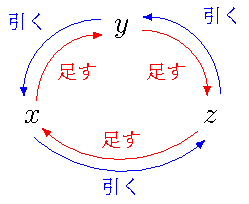
\includegraphics[width=5cm]{picture/vecter4.pdf}
 \caption{外積の成分表示の覚え方}
\end{figure}

$\bm{a} \times \bm{b}$を求めたいときは,
成分を$\bm{a}$のもの,$\bm{b}$のもの,$\bm{a}$のもの,$\bm{b}$のもの,$\cdots$と取り出していく.
図に書いたのは添え字のパターンである.

まず$x$成分からスタートである.一番上の$y$からスタートする.そして右下の$z$に移る.$y, \, z$という添え字の配列が与えられる.
こうして$a_y b_z$というものが与えられる.次に添え字を入れ替えて引くのだ.$a_y b_z - a_z b_y$となる.
これは外積$\bm{a} \times \bm{b}$の$x$成分であった.

次に$y$成分である.さっき進んだ$z$からスタートだ.添え字の配列は$x$に向かって$z, \, x$とする.
そして$a_z b_x$のいうものが得られた.
そして添え字を入れ替えて引くのだ.$a_z b_x - a_x b_z$となり,これは外積$\bm{a} \times \bm{b}$の$y$成分であった.

$z$成分も同様である.外積$\bm{a} \times \bm{b}$の$z$成分は$a_x b_y - a_y b_x$であった.

小難しく図の読み方を書いたが,図を見てどう読むかが直感的にわかったのならそれでいい.とにかく覚えられればいいのだ.

外積に関してはこんなものである.特に難しいところはなかった.わかってしまえばなんてことはないのである.
\begin{itembox}[l]{課題}
3次元数ベクトル空間における標準基底
$$
\bm{e}_x = \left[
 \begin{array}{c}
 1 \\
 0 \\
 0 
 \end{array}
\right]
\: ,\: 
\bm{e}_y = \left[
 \begin{array}{c}
 0 \\
 1 \\
 0 
 \end{array}
\right]
\: ,\: 
\bm{e}_z = \left[
 \begin{array}{c}
 0 \\
 0 \\
 1 
 \end{array}
\right]
$$
について,それらの外積を考える.このとき
$$
\bm{e}_x \times \bm{e}_y = \bm{e}_z \; , \; 
\bm{e}_y \times \bm{e}_z = \bm{e}_x \; , \; 
\bm{e}_z \times \bm{e}_x = \bm{e}_y 
$$
が成り立っていることを
\begin{enumerate}
\item 幾何学的定義に基づいて向きと大きさを求める
\item 成分表示の公式により外積の各成分を直接計算する 
\end{enumerate}
この2つの方法によって確かめよ.

また,2つのベクトル
$$
\bm{a} = \left[
 \begin{array}{c}
  a_x \\ 
  a_y \\
  a_z
 \end{array}
\right]
\; , \; 
\bm{b} = \left[
 \begin{array}{c}
  b_x \\ 
  b_y \\
  b_z
 \end{array}
\right]
$$
と上に述べた標準基底に対して,等式
\begin{align}
\bm{a} \times \bm{b} = \left| 
\begin{array}{ccc}
 \bm{e}_x & \bm{e}_y & \bm{e}_z \\
 a_x & a_y & a_z \\
 b_x & b_y & b_z 
\end{array}
\right|
\label{eq:gaisekidet}
\end{align}
が成り立っていることを確かめよ.ただし右辺の$\lvert \, \cdot \, \rvert$
は行列式を表す.

さらに,3つのベクトル$\bm{a}, \, \bm{b}, \, \bm{c}$について,結合律
\begin{align}
( \bm{a} \times \bm{b} ) \times \bm{c} =\bm{a} \times ( \bm{b} \times \bm{c} )
\end{align}
が成り立っているかどうか検証せよ.

結合律のついでに,交換律や分配律が
内積や外積においてはどうなっているか調査せよ.
\end{itembox}
\section{ベクトル空間の基底とその変換}
さっき``標準基底''という言葉が出てきた.
それらは空間内に存在するベクトルをすべて標準基底を用いて表すことができるのであった.
しかし,空間内のベクトルを表現することに標準基底を用いなければいけないわけではない.
このことについて考えたいのだが,先に少し下準備をしておく.
\subsection{ベクトル空間とは何か}
いままで出てきたのは,$n$次元数ベクトル空間というひどく抽象化されたよくわからない空間であった.
$1,\, 2, \, 3$次元くらいならイメージがつくが,それ以上になるともはや頭の中ではイメージ不可能なものであった.
しかし,ここには大きな落とし穴が潜んでいる.実は,$n$次元数ベクトル空間の``空間''と,
我々が常日頃使っている\footnote{一般の日常生活でという意味である.}``空間''はまったく別物なのである.
いや,さすがに言い過ぎである.
正確には,数学者のいう空間は,我々が空間といってイメージする概念をさらに抽象化したものであるというべきだろうか.

集合に,なんらかの数学的構造を付与したものを\emph{空間}という.
そして,集合に和とスカラー倍という数学的構造を付与したものを\emph{ベクトル空間}
\index[widx]{べくとるくうかん@ベクトル空間}
もしくは\emph{線形空間}\index[widx]{せんけいくうかん@線形空間|see{ベクトル空間}}
と呼ぶ.
数学的構造というとなんとなく難しく聞こえるが,誤解を恐れずにいってしまうと,
数学的構造とはなんらかの``仕組み''である.
ベクトルの演算として,和とスカラー倍というのがあった.
あのような演算ができなければベクトル空間とは言わない.
和やスカラー倍という``仕組み''は数学者的には代数的構造に分類されるらしい.
そういえば,ベクトル空間の性質を探るのは線形代数学の役目であり,
線形代数学には代数学という名前がついているのであった.
こうなると,普通の幾何ベクトルだけでなく,
もっとたくさんの集合がベクトル空間として扱えそうである.
モノの中身でなく,モノが示す性質について議論しているがためにこういうことが言える.
線形代数学の理論がいろいろなところで顔を出すのはこのためである.
いろんな分野で扱う概念にベクトル空間と同じような代数構造を持っているがために,
ベクトル空間の理論を使ってそれらの分野の研究ができるのである.
ただし,物理学では,ベクトル空間にさらに内積と呼ばれる代数構造を付与したものを扱うのが普通である.
内積が付与されたベクトル空間は\emph{計量ベクトル空間}
\index[widx]{べくとるくうかん@ベクトル空間!けいりょう@計量---|see{内積空間}}もしくは
\emph{内積空間}\index[widx]{ないせきくうかん@内積空間}と呼ばれる.
詳しいことは省くが,内積という演算を導入することにより,
ベクトルの長さやなす角といった概念を考えることができるのである.
以前述べた内積のところを読み返してみれば,
ベクトルの長さやなす角(の余弦)といった概念に内積が関与していることがわかるはずだ.

これからはただの数ベクトル空間ではなく一般のベクトル空間の話をするが,
ほとんど普通の数ベクトル空間だと思って解釈してもらって構わない.
そういうことができるよううまいこと理論が組まれているのである.
\subsection{線形結合と線形独立}
2つのベクトル$\bm{a}, \, \bm{b}$とスカラー$p, \, q$について,
\begin{align}
p\bm{a}+q\bm{b}
\label{eq:senkeiketugou}
\end{align}
と表されるベクトルを$\bm{a}$と$\bm{b}$の($p, \, q$を係数とする)\emph{線形結合}
\index[widx]{せんけいけつごう@線形結合}
もしくは\emph{$1$次結合}
\index[widx]{いちじけつごう@1次結合|see{線形結合}}という.
形が何となく比例の式に似ている.比例式はグラフにすると直線を表すので``線形''と呼ばれているのである.
本書は線形結合という呼称を用いることにする.
また,$n$本のベクトル$\bm{v}_1, \, \bm{v}_2, \, \cdots, \, \bm{v}_n$
と$n$個のスカラー$c_1, \, c_2, \, \cdots, \, c_n$について,
\begin{align}
c_1 \bm{v}_1 + c_2 \bm{v}_2 + \cdots + c_n \bm{v}_n
\label{eq:nsenkeiketugou}
\end{align}
と書き表されるベクトルを$\bm{v}_1, \, \bm{v}_2, \, \cdots , \, \bm{v}_n$の
($c_1, \, c_2, \, \cdots, \, c_n$を係数とする)\emph{線形結合}という.
線形結合は,線形代数学の理論の中核をなす非常に重要な概念である.
よく``このベクトルを別のベクトルで表す''ということがあるが(本書でもすでに散々使っている),
これは線形結合で表せるという意味で使うことがほとんどである.
例えば,3次元数ベクトル空間の標準基底$ \{ \, \bm{e}_1, \, \bm{e}_2, \, \bm{e}_3 \, \} $を考えてみる.
ベクトルの外積を用いると,$\bm{e}_3$は$\bm{e}_3 = \bm{e}_1 \times \bm{e}_2$と表せる.
しかし,このような場合,``$\bm{e}_3$は$\bm{e}_1$と$\bm{e}_2$で表せる''とは普通は言わない.
線形結合以外の方法を使っているからである.
$\bm{e}_3$は$\bm{e}_1$と$\bm{e}_2$では表せない.それだけではなく,
$\{ \, \bm{e}_1, \, \bm{e}_2, \, \bm{e}_3 \, \}$からどのベクトルを取り出してきても,
そのベクトルを残った2つのベクトルを用いては表せない.
これを確かめるのは簡単であるから,読者の方々の練習問題としよう.

さて,この``線形結合では表せない''ということについてもう少し考えてみよう.
2つのベクトル$\bm{v}_1, \, \bm{v}_2$について,$\bm{v}_2$が$\bm{v}_1$の線形結合で表せるというのは,
スカラー$c$をうまくとって,$\bm{v}_2 = c \bm{v}_1$が成り立つということである.
式(\ref{eq:nsenkeiketugou})はベクトルが複数あるが,いまは1つのベクトルだけで線形結合というものを考えている.
この場合は$c \bm{v}_1$というただのスカラー倍に相当するわけだ.
ベクトルのスカラー倍というのはベクトルが表現する矢印を伸ばしたり縮めたりするようなイメージであった.
従って,$\bm{v}_2$が$\bm{v}_1$の線形結合で表せるというのは,$\bm{v}_1$と$\bm{v}_2$の向きが同じであるか,
違ったとしても向きが真逆であるかのどちらかである.
この場合,``$\bm{v}_1$と$\bm{v}_2$を用いて別のベクトルを表現する''という観点では
2本もベクトルはいらないということに
なる.\footnote{この``表現する''ももちろん線形結合で表現するという意味である.}
このとき,$\bm{v}_1$と$\bm{v}_2$の線形結合全体の集合は,ある種の直線のような集合になる.
よって,この集合は1次元のベクトル空間であるといわれるのだ.
次元についてはあとで詳しくやろう.

次に,$\bm{v}_2$が$\bm{v}_1$の線形結合で表せないとしよう.
この場合,$\bm{v}_1$と$\bm{v}_2$の向きはまったく違うことになる.違うといっても正反対ではあってはならない.
``$\bm{v}_1$と$\bm{v}_2$を用いて別のベクトルを表現する''という観点で考えてみると,
この2つのベクトルは$\bm{v}_1$と$\bm{v}_2$の貼る
平面\footnote{内積のところで``2つのベクトルが貼る平行四辺形''というのをやったが,それと同じイメージである.}
内に存在するベクトルすべてを表すことができる.
しかし,ひとたびその平面から飛び出てしまったベクトルは,$\bm{v}_1$と$\bm{v}_2$では表せない.
平面を表すので,このベクトル空間は2次元であるといわれるのである.
また,$\bm{v}_1$と$\bm{v}_2$が貼る平面から飛び出すようなベクトル$\bm{v}_3$をとり,
$\bm{v}_1, \, \bm{v}_2, \, \bm{v}_3$の3本のベクトルの線形結合全体からなる集合を考えると,
この集合は空間上のあらゆる点全部の集合である.
というわけで,このベクトル空間は3次元であるといわれる.

\subsection{ベクトル空間の基底と次元}
ここまでもったいぶって引っ張ってきた線形独立性について話をしよう.
\begin{itembox}[l]{定義}
$n$本のベクトル$ \bm{v}_1, \, \bm{v}_2, \, \cdots, \, \bm{v}_n $について,
\begin{align}
c_1 \bm{v}_1 + c_2 \bm{v}_2 + \cdots + c_n \bm{v}_n = 0
\label{eq:senkeidokuritu}
\end{align}
を成り立たせるスカラー$c_1, \, c_2, \, \cdots , \, c_n$が$c_1=c_2=\cdots=c_n=0$以外にないとき,
$ \bm{v}_1, \, \bm{v}_2, \, \cdots, \, \bm{v}_n $は
\emph{線形独立}\index[widx]{せんけいどくりつ@線形独立}
であるといい,式(\ref{eq:senkeidokuritu})を成り立たせる
スカラー$c_1, \, c_2, \, \cdots , \, c_n$が$c_1=c_2=\cdots=c_n=0$以外に存在するとき,
$ \bm{v}_1, \, \bm{v}_2, \, \cdots, \, \bm{v}_n $は
\emph{線形従属}\index[widx]{せんけいじゅうぞく@線形従属}であるという.
\end{itembox}
線形独立と線形従属はそれぞれ1次独立,1次従属とも呼ばれる.これは線形結合と同じである.
さっきまでの話とずいぶん趣が違うように見えるがそれは表現上の都合である.
それを象徴するような定理がある.
\begin{itembox}[l]{定理}
$n$本のベクトル$ \bm{v}_1, \, \bm{v}_2, \, \cdots, \, \bm{v}_n $について,
$ \bm{v}_1, \, \bm{v}_2, \, \cdots, \, \bm{v}_n $が線形独立であるための必要十分条件は,
$ \bm{v}_1, \, \bm{v}_2, \, \cdots, \, \bm{v}_n $の中からどのベクトルをとっても,
そのベクトルが残ったベクトルの線形結合で書き表せないことである.
\end{itembox}
この定理の証明もあまり難しくないので読者への課題としておこう.
線形独立のイメージとしては今述べた定理のようなイメージであるが,
数学の議論を進めていくうえで使いやすいのは定義で述べた方である.
しかし,どちらも同じことだよというのが数学の議論によって証明できるので,
どちらを定義として採用しても構わない.
実際,定理として述べた上の命題を定義として採用している本も多い.
また,これまでの議論から,次元と線形独立性が非常に深く関係していることが見て取れる.

さて,我々は``次元''という言葉をあいまいに使ってきた.そこで,次元という言葉を正確に定義しておこう.
\begin{itembox}[l]{定義}
ベクトル空間$V$と,$V$の$n$本のベクトル$ \bm{v}_1, \, \bm{v}_2, \, \cdots, \, \bm{v}_n $について,
$ \bm{v}_1, \, \bm{v}_2, \, \cdots, \, \bm{v}_n $が線形独立で,かつ
$V$のどんなベクトルも$ \bm{v}_1, \, \bm{v}_2, \, \cdots, \, \bm{v}_n $の線形結合で表せるとき,
$ \bm{v}_1, \, \bm{v}_2, \, \cdots, \, \bm{v}_n $は$V$の\emph{基底}
\index[widx]{きてい@基底}
である,もしくは単に\emph{基}といい,$V$は\emph{$n$次元}ベクトル空間であるという.
\end{itembox}
我々がいままでなんとなく使ってきた``次元''という言葉は,
ベクトル空間のなかのベクトルを表現するのに必要な最低限のベクトルの本数だということになる.
\footnote{しかし,我々はもうひとつ別の``次元''という言葉の使い方を知っている.}
``必要''が$V$のどんなベクトルもの部分に対応し,``最低限''が線形独立性に対応している.
上に書いた無機質で数学チックな``次元''の定義がいままで何も考えずに使っていた``次元''という言葉の
ニュアンスとぴったり合致していることはわかるだろうか? 我々が生きているこの世界が
ベクトル空間であるかどうかに関しては疑問の余地は大いにあるが,
そういう細かいことを無視すれば,``次元''という言葉のイメージと厳密な定義がぴったり一致したはずである.
なお,先ほど述べた定義は暗に次元が有限であることを前提にしている.
有限個の基底をとることができないような無限次元のベクトル空間も確かに存在してはいるのだが,
そういう話をしだすとめんどくさいのでここでは述べない.
近いうちに出会うことになるだろうからそのときに学んでもらえばいい.

もうひとつ重要な話をしなければならない.
それは,ベクトル空間が与えられたとき,
その基底の取り方は何通りも考えられるということである.
これは結構重要な事実である.
例を出して考えよう.3次元数ベクトル空間$\mathbb{R}^3$において,
\footnote{数ベクトル空間を表すときはこういう変な文字を使う.
手書きではベクトルと同じように2重文字で書いておけばよい.}
標準基底
\begin{align*}
\bm{e}_1 = \left[
 \begin{array}{c}
  1 \\ 
  0 \\
  0
 \end{array}
\right]
\; , \, \; 
\bm{e}_2 = \left[
 \begin{array}{c}
  0 \\ 
  1 \\
  0
 \end{array}
\right]
\; , \; 
\bm{e}_3 = \left[
 \begin{array}{c}
 0 \\
 0 \\
 1
 \end{array}
\right]
\end{align*}
はもちろん$\mathbb{R}^3$の基底である.だが,
\begin{align*}
\bm{a}_1 = \left[
 \begin{array}{c}
  1 \\ 
  1 \\
  0
 \end{array}
\right]
\; , \, \; 
\bm{a}_2 = \left[
 \begin{array}{c}
  0 \\ 
  1 \\
  1
 \end{array}
\right]
\; , \; 
\bm{a}_3 = \left[
 \begin{array}{c}
 1 \\
 0 \\
 1
 \end{array}
\right]
\end{align*}
としてみるとこれら$ \{ \, \bm{a}_1, \, \bm{a}_2, \, \bm{a}_3 \, \} $も$\mathbb{R}^3$の基底になっている.
本当に基底になっているかどうか確かめる作業は読者にゆだねよう.そんなに難しい話ではない.
基底の取り方はいろいろあるが,
同じベクトル空間であるならば基底の数は取り方によらず一定であることが知られている.
あるベクトル空間$V$において,とある基底をとってみたら4本だったが,
別の取り方をしてみたら3本でしたということはあり得ない.
ベクトル空間の次元は基底の取り方には依存しないのである.
もし依存するようなことがあれば,ベクトル空間の次元は基底ごとに変化するということになってしまう.
このようなことは直感的に考えてもあり得なさそうだということはわかるだろう.
この事実は数学的に証明できるものであるが本書ではスキップしておく.

さらに1つ補足をしておく.$n$次元ベクトル空間$V$の基底を1つとり,
$V$のベクトルをその基底の線形結合として表したとき,その表し方は一意である.
これは直感的にも納得できるだろう.もちろん数学的にも簡単に証明できる.

そういえば,$ \{ \, \bm{e}_1, \, \bm{e}_2, \, \bm{e}_3 \, \} $は$\mathbb{R}^3$の基底であって,
$ \{ \, \bm{a}_1, \, \bm{a}_2, \, \bm{a}_3 \, \} $も同じ$\mathbb{R}^3$の基底であった.
従って,互いは互いの線形結合で表せるはずである.
実際,
\begin{align*}
\bm{a}_1 = 1 \bm{e}_1 + 1 \bm{e}_2 + 0 \bm{e}_3 \\
\bm{a}_2 = 0 \bm{e}_1 + 1 \bm{e}_2 + 1 \bm{e}_3 \\
\bm{a}_3 = 1 \bm{e}_1 + 0 \bm{e}_2 + 1 \bm{e}_3 
\end{align*}
となる.ここで,行列$A$を
\begin{align*}
A= \left[
\begin{array}{ccc}
1 & 0 & 1 \\
1 & 1 & 0 \\
0 & 1 & 1
\end{array}
\right] 
\end{align*}
と定めてみると,
\begin{align}
\left[
\begin{array}{ccc}
\bm{a}_1 & \bm{a}_2 & \bm{a}_3 
\end{array}
\right]
= 
\left[
\begin{array}{ccc}
\bm{e}_1 & \bm{e}_2 & \bm{e}_3
\end{array}
\right]
A
\label{eq:ahenkan}
\end{align}
という関係式が成り立つ.
この式は,行列の積のルールにのっとった関係式
\begin{align*}
\left[
\begin{array}{ccc}
1 & 0 & 1 \\
1 & 1 & 0 \\
0 & 1 & 1 
\end{array}
\right]
= 
\left[
\begin{array}{ccc}
1 & 0 & 0 \\
0 & 1 & 0 \\
0 & 0 & 1 \\
\end{array}
\right]
\left[
\begin{array}{ccc}
1 & 0 & 1 \\
1 & 1 & 0 \\
0 & 1 & 1
\end{array}
\right]
\end{align*}
というところからきている.
それぞれのベクトルや行列の成分を代入してみればすぐにわかるはずだ.
行列$A$の定義が列と行が逆に見えたのは,各列ベクトルを横に配置しているからである.
関係式を並べるときには各ベクトルを縦に並べ,さも1つの未知数であるかのように表した.
連立方程式を行列で表記したのと同じように見せるためだ.
しかし,いま扱っているモノは未知数ではなくベクトルである.
そういう場合には違う表記をした方が都合がいい.
まぁどう都合がいいかを説明しろと言われると困るのだが.
ともかく,この関係式はこの後すぐに使うので頭の片隅にでも置いておいてほしい.
\subsection{基底の変換}
ここまで長々とおおよそ物理と関係のなさそうなことを述べてきたのはもちろんわけがある.
抽象的な数学が何を目指しているかを知ってほしいというのも1つであるが,
最大の目的は基底の変換という概念をマスターすることにある.
さっき述べた話とつながるのだが,復習を兼ねてもう一度最初から説明してみよう.
ただし,もはや扱うのは数ベクトルではなく一般のベクトルだ.

あるベクトル空間$V$があったとする.$\bm{v}_1, \, \bm{v}_2, \, \cdots , \, \bm{v}_n$を$V$の基底として取ろう.
しかし,基底の取り方は1通りではない.取り方はいくらでも考えられるのであった.
例えばそれを$\bm{v}'_1, \, \bm{v}'_2, \, \cdots , \, \bm{v}'_n$としてみよう.
基底の取り方はいろいろあるが,その本数は変わらないのだった.
というわけでさっきと同じく$n$本である.
さて,$\bm{v}_1, \, \bm{v}_2, \, \cdots , \, \bm{v}_n$と$\bm{v}'_1, \, \bm{v}'_2, \, \cdots , \, \bm{v}'_n$
は,同じベクトル空間$V$の基底である.
従って,互いは互いの線形結合で表せるはずである.
つまり,$n^2$個のスカラー
$p_{11}, \, p_{12}, \, \cdots, \, p_{1n}, \, p_{21}, \, p_{22}, \, \cdots, \, p_{2n}, \, \cdots, \,  p_{nn}$
をうまく選んで
\begin{align}
\begin{aligned}
\bm{v}'_1 & = p_{11} \bm{v}_1 + p_{21} \bm{v}_2 + \cdots + p_{n1} \bm{v}_n \\
\bm{v}'_2 & = p_{12} \bm{v}_1 + p_{22} \bm{v}_2 + \cdots + p_{n2} \bm{v}_n \\
& \hspace{2.3cm }\vdots \\
\bm{v}'_n & = p_{1n} \bm{v}_1 + p_{2n} \bm{v}_2 + \cdots + p_{nn} \bm{v}_n 
\end{aligned}
\label{eq:nanka}
\end{align}
という$n$個の関係式を成立させることができるはずである.
なんだかどこかで見た形である.そこで,$n$次の正方行列$P$を
\begin{align*}
P =
\left[
\begin{array}{cccc}
p_{11} & p_{12} & \ldots & p_{1n} \\
p_{21} & p_{22} & \ldots & p_{2n} \\
\vdots & \vdots & \ddots & \vdots \\
p_{n1} & p_{n2} & \ldots & p_{nn}
\end{array}
\right]
\end{align*}
と定めてみる.
すると,式(\ref{eq:nanka})は次のように変形できる.
\begin{align}
( \bm{v}'_1, \, \bm{v}'_2, \, \cdots, \bm{v}'_n ) = ( \bm{v}_1, \, \bm{v}_2, \, \cdots, \bm{v}_n ) P
\label{eq:henkan}
\end{align}
この話は以前にもやった話である.以前の話と違うのは,ベクトルが$n$本あるということと,
扱っているのが数ベクトルではなく一般のベクトルだということである.
そういうわけで,ベクトルをまとめるカッコが$[ \cdots ]$ではなく$( \cdots )$になっている.
このカッコはとりあえず行列を表すカッコと同じように解釈してくれて構わない.
式(\ref{eq:henkan})は以前やった式(\ref{eq:ahenkan})とほとんど同じことを表しているというわけだ.

さて,ここからが話の核心である.式(\ref{eq:henkan})を作ったときは
``すでに基底が2組与えられていて,それらを行列が結びつけている''というイメージであった.
しかし,こう解釈できないだろうか? すでに基底
$ \{ \bm{v}_1, \, \bm{v}_2, \, \cdots, \, \bm{v}_n \} $と行列$P$が与えられていて,
それを用いて新しい基底$ \{ \bm{v}'_1, \, \bm{v}'_2, \, \cdots, \, \bm{v}'_n \} $を作り出した
のだと解釈してみるのである.
このように考えてみると,行列$P$は基底$ \{ \bm{v}_1, \, \bm{v}_2, \, \cdots, \, \bm{v}_n \} $
を別の基底$ \{ \bm{v}'_1, \, \bm{v}'_2, \, \cdots, \, \bm{v}'_n \} $
に変換するような行列であるとイメージできる.
というわけで,この行列$P$を基底$ \{ \bm{v}_1, \, \bm{v}_2, \, \cdots, \, \bm{v}_n \} $
から基底$ \{ \bm{v}'_1, \, \bm{v}'_2, \, \cdots, \, \bm{v}'_n \} $への\emph{変換行列}
\index[widx]{きてい@基底!のへんかんぎょうれつ@---の変換行列}と名付けよう.
この基底の変換は,そのまま座標変換の話につながってくる.
基底と座標は深くつながっているのである.このことについて考えてみよう.
\section{座標系とその変換}\label{zahyoukei}
\label{sec:zahyoukei}
$n$次元のベクトル空間$V$において,その基底を1つとり,$ \{ \bm{v}_1, \, \bm{v}_2, \, \cdots, \, \bm{v}_n \} $
すると,$V$内の任意のベクトル$\bm{a}$はこれらの基底の線形結合で表せる.
その線形結合を
\begin{align}
\bm{a} = a_1 \bm{v}_1 + a_2 \bm{v}_2 + \cdots + a_n \bm{v}_n 
\label{eq:ketugou}
\end{align}
としてみる.式(\ref{eq:ketugou})中の係数の組$(a_1, \, a_2, \, \cdots , \, a_n)$を
$\bm{a}$の基底$ \{ \bm{v}_1, \, \bm{v}_2, \, \cdots, \, \bm{v}_n \} $に関する
\emph{座標}\index[widx]{ざひょう@座標}
と呼ぶ.
ここに使われている``座標''という言葉は,$n$次元数ベクトル空間$\mathbb{R}^n$において,
我々がこれまで使っていた``座標''とほとんどまったく同じ意味である.
基底として,標準基底$ \{ \, \bm{e}_1, \, \bm{e}_2, \, \cdots , \, \bm{e}_n \, \} $をとれば,
ベクトル$\bm{a} = \left[
\begin{array}{c}
a_1 \\
a_2 \\
\vdots \\
a_n
\end{array}
\right]
$は
\begin{align*}
\bm{a} = a_1 \bm{e}_1 + a_2 \bm{e}_2 + \cdots + a_n \bm{e}_n
\end{align*}
と表されるので,$\bm{a}$の標準基底$ \{ \bm{e}_1, \, \bm{e}_2 , \, \cdots , \, \bm{e}_n \} $に関する座標は
$( a_1, \, a_2, \, \cdots , \, a_n)$ということになる.数ベクトル空間の概念を導入したときと同じようなイメージである.
あのときは$\mathbb{R}^n$の基底を標準基底とするということが暗黙のうちに了解されていたのである.

さて,ここからが面白いところである.同じベクトル空間であっても,その基底の取り方はいろいろあったのだった.
同じベクトルであっても,選ぶ基底が変わればその基底に関する座標は変化する.
つまり,基底を選択することは,その空間でどのような座標系を導入するかに相当するのである.
ここでは,物理でよく使う2次元と3次元数ベクトル空間$\mathbb{R}^2, \, \mathbb{R}^3$
のいろいろな座標系について考えてみよう.
\subsection{2次元空間における座標系}
空間内の座標を決定するためのシステムのことを\emph{座標系}\index[widx]{ざひょうけい@座標系}
と呼ぶ.
座標系は,ほとんど基底と同じようなイメージである.
そして,ある座標系から別の座標系に乗り換えることを\emph{座標変換}
\index[widx]{ざひょう@座標!へんかん@---変換}と呼ぶ.
今回主題になるのは,座標系にはどういうものがあって,それぞれがどういう関係で結びついているかということである.
物理でよく使う座標系にはいくつか種類がある.
寄り道をしながらひとつひとつゆっくり見ていこう.
\subsubsection{直交直線座標系}
まずは2次元空間における座標系について考えよう.2次元に対して``空間''という言い方はあまりしなくて,
普通2次元平面というように呼ばれるのであった.
そういえば,我々はよくこの平面のことを\emph{$xy$平面}というように呼ぶのだった.
なぜかというと,我々は通常右向きに$x$軸,上向きに$y$軸を置き,
それに従って平面上の点\footnote{点の位置を決めることと,
ベクトルを1つ決めることは本質的にはほとんど変わらないというのは以前話したことである.}
の位置を判断しているからだ.
このような点の位置の決め方のルールを採用することは座標系を導入するというのだった.
この場合,このルールの象徴は$x$軸と$y$軸という2本の直交する直線である.
ゆえに,いま採用したこの座標系は\emph{直交直線座標系}
\index[widx]{ざひょうけい@座標系!ちょっこうちょくせん@直交直線---|see{Descartes座標系}}と呼ばれている.
偉そうに直交だの直線だの言っているのはそうでない座標系があるからだ.
\begin{figure}[h]
 \begin{center}
 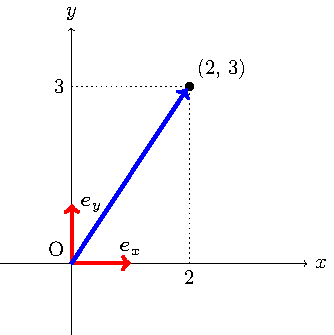
\includegraphics[width=5.5cm]{picture/vecter8.pdf}
 \caption{直交直線座標系における標準基底}
 \end{center}
\end{figure}

さて,この座標系に対応するような基底の取り方というのはもちろん標準基底のことである.
例えば点$(2, \, 3)$といえば,これは原点から右向きに2,上向きに3だけ進んだような点を表すのだった.
これはちょうど位置ベクトル$\left[ 
\begin{array}{c}
2 \\
3
\end{array}
\right] $に相当し,このベクトルは標準基底$ \{ \, \bm{e}_x, \, \bm{e}_y \, \} $を使えば
$2\bm{e}_x+3\bm{e}_y$と表せるのであった.さっきまでと標準基底の添え字の使い方を変えているが,
これは$xy$平面という言葉に引きずられてそうなっている.

この座標系を考案したのはDescartesという人物である.
そういうわけで,直交直線座標系のことを\textbf{Descartes座標系}
\index[widx]{ざひょうけい@座標系!Descartes@Descartes---}
\index[nidx]{Descartes@Descartes(デカルト)}
と呼ばれることも多い.人名が付いた用語というのはなんとなくかっこいいものである.
英語圏では``Descartesの''という意味を表す形容詞としてCartesian(カーテシアン)
という用語がある.そういうわけで,海外での生活が長い人などはDescartes座標系ではなく
\textbf{Cartesian座標系}
\index[widx]{ざひょうけい@座標系!Cartesian@Cartesian---|see{Descartes座標系}}
などと呼ぶこともあるそうだ.

\subsubsection{斜交直線座標系}
座標系の取り方はもちろんDescartes座標系だけではない.
``直交直線座標系''というところから``直交''という要素を取り払ってみよう.

座標軸の引き方は,さっきと同じく直線を2本引くのだが,
この線の引き方は平行でもなければもはや自由である.
線の引き方表現するかについてであるが,
引いた直線と同じ向きのベクトルを2本用意してみよう.
そして,$\bm{a}$方向と$\bm{b}$方向に直線を引き,その2本の直線を座標軸としてみる.
例えばそれを$\bm{a}, \, \bm{b}$として,``私は$\bm{a}$方向と$\bm{b}$方向を軸にします''といっておけばいいのである.
こういう場合,引いた直線のことを$\bm{a}$軸,$\bm{b}$軸などというように呼ぶこともある.
$\bm{a}$と$\bm{b}$はもちろん線形独立で,$\mathbb{R}^2$の基底になる.
そして,平面上のベクトルを$\bm{a}$と$\bm{b}$の線形結合で表したときの係数がそのベクトルの
基底$\{ \, \bm{a}, \, \bm{b} \, \} $に関する座標ということになる.
すなわち,$\bm{a}, \, \bm{b}$という2本のベクトルを用意することにより,
座標を決定するための規則,つまり座標系が与えられたことになる.
このように,直交せず,かつ平行でない2本の直線を基準とした座標系を
\emph{斜交直線座標系}\index[widx]{ざひょうけい@座標系!しゃこうちょくせん@斜交直線---}と呼ぶ.

例を出して考えてみよう.Descartes座標系で表したときの成分表示が$\left[
\begin{array}{c} 
\displaystyle \frac{1}{4} \\
1
\end{array} 
\right]$
になるようなベクトルを$\bm{a}$,
$\left[
\begin{array}{c}
1 \\ 
\displaystyle \frac{1}{4} 
\end{array} 
\right]$
になるようなベクトル$\bm{b}$を考え,これらを基準とした斜交直線座標系を導入する.
この座標系における座標が$\left( \displaystyle \frac{8}{3}, \, \frac{4}{3} \right)$
となるような点の様子は図\ref{fig:syakou}
のようになる.
\begin{figure}[h]
 \begin{center}
 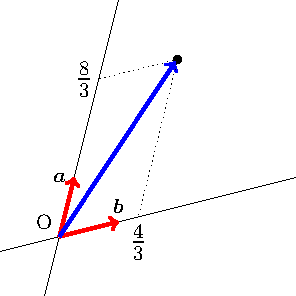
\includegraphics[width=4.8cm]{picture/vecter9.pdf}
 \caption{斜交直線座標系とその基底}
\label{fig:syakou}
 \end{center}
\end{figure}
\\
この座標系における座標が$\left( \displaystyle \frac{8}{3}, \, \frac{4}{3} \right)$
となるような点に対応する位置ベクトルは
$ \displaystyle \frac{8}{3} \bm{a} + \frac{4}{3} \bm{b} $と書き表されるというわけだ.
この点をDescartes座標系で表すとどうなるだろうか? これはとても簡単で,
$\bm{a}$と$\bm{b}$をDescartes座標系で表してやって計算すればいいのであり,
\begin{align*}
\frac{8}{3} \bm{a} + \frac{4}{3} \bm{b} & = \frac{8}{3} \left( \frac{1}{4} \bm{e}_x + 1 \bm{e}_y \right)
+ \frac{4}{3} \left( 1 \bm{e}_x + \frac{1}{4} \bm{e}_y \right) \\
& = \frac{2}{3} \bm{e}_x + \frac{8}{3} \bm{e}_y + \frac{4}{3} \bm{e}_x +\frac{1}{3} \bm{e}_y \\
& = 2 \bm{e}_x + 3 \bm{e}_y
\end{align*}
となって,この点の座標をDescartes座標系で表すと$(2, \, 3)$となるということがわかる.
つまり,さっきの座標系で座標が$\left( \displaystyle \frac{8}{3}, \, \frac{4}{3} \right) $となるような点と,
Descartes座標系で座標が$(2, \, 3)$となるような点は同じ点なのだ.
座標系を変えれば点を表す座標も変わるのである.
このことには注意を払わねばなるまい.しかし,通常は点$(2, \, 3)$といえば,
これはDescartes座標系での座標が$(2, \, 3)$であるような点を表す.
違う座標系を用いるときはその都度断るのが原則である.
この文章もそういうように気を付けて書いてあるはずだ.

基底$\{ \, \bm{e}_x, \, \bm{e}_y \, \} $から基底$ \{ \, \bm{a}, \, \bm{b} \, \} $の変換行列を求めてみよう.
$\bm{a}$と$\bm{b}$は$\bm{e}_x, \, \bm{e}_y$を用いて
\begin{align*}
\bm{a} & = a_x \bm{e}_x + a_y \bm{e}_y \\
\bm{b} & = b_x \bm{e}_x + b_y \bm{e}_y
\end{align*}
と表せる.本当は$a_x$や$b_y$などといった値はわかっているのだが,
いまは式を一般的に考えるためにあえて値を文字にしている.
この式から,2次の正方行列$P$を
\begin{align*}
P= 
\left[
\begin{array}{cc}
a_x & b_x \\
a_y & b_y 
\end{array}
\right]
\end{align*}
と定めれば,
\begin{align*}
\left[
\begin{array}{cc}
\bm{a} & \bm{b} 
\end{array}
\right]
=
\left[
\begin{array}{cc}
\bm{e}_x & \bm{e}_y
\end{array}
\right]
P
\end{align*}
という関係式が成り立っていることになる. 
つまり,基底$\{ \, \bm{e}_x, \, \bm{e}_y \, \} $から基底$ \{ \, \bm{a}, \, \bm{b} \, \} $の変換行列$P$は
\begin{align*}
P=
\left[
\begin{array}{cc}
\bm{a} & \bm{b}
\end{array}
\right]
\end{align*}
ということになる.ちょうど基底を2本並べた形になっている.
この行列$P$は基底同士の関係を表す行列である.

ところで,我々が普段目にしているのは座標同士の関係式である.
それを求めてみよう.

Descartes座標系での座標が$(x, \, y)$になるような点の位置ベクトルを$\bm{r}$とする.
$\bm{r}$を$\bm{a}, \, \bm{b}$というベクトルを基準とした斜交直線座標系で表したときに,
その座標が$(x', \, y')$になったとする.$x, \, y$と$x', \, y'$の関係式を求めたい.
$\bm{a}, \, \bm{b}$は標準基底を用いて
\begin{align*}
\bm{a} & = a_x \bm{e}_x + a_y \bm{e}_y \\
\bm{b} & = b_x \bm{e}_x + b_y \bm{e}_y
\end{align*}
と書き表せるとしよう.$\bm{r}$をそれぞれの座標系で表すと
\begin{align*}
\bm{r} & = x \bm{e}_x + y \bm{e}_y \\
\bm{r} & = x' \bm{a} + y' \bm{b} 
\end{align*}
となる.この式で$\bm{r}$は同じ1つのベクトルなので
\begin{align*}
x' \bm{a} + y' \bm{b} = x \bm{e}_x + y \bm{e}_y 
\end{align*}
となる.ここから$\bm{a}, \, \bm{b}$を消去してやると
\begin{align*}
x' ( a_x \bm{e}_x + a_y \bm{e}_y ) + y' ( b_x \bm{e}_x + b_y \bm{e}_y ) & = x \bm{e}_x + y \bm{e}_y \\
\therefore (a_x x' + b_x y' ) \bm{e}_x  + ( a_y x' + b_y y' ) \bm{e}_y & = x \bm{e}_x + y \bm{e}_y
\end{align*}
標準基底$\bm{e}_x, \, \bm{e}_y$はもちろん線形独立であるから
\begin{align*}
a_x x' + b_x y' & = x \\
a_y x' + b_y y' &= y
\end{align*}
ということになる.さっきの行列$P$を使ってみると
\begin{align*}
P 
\left[
\begin{array}{c}
x' \\
y'
\end{array}
\right]
= 
\left[
\begin{array}{c}
x \\
y
\end{array}
\right]
\end{align*}
となる.$P$の逆行列$P^{-1}$を用いれば
\begin{align*}
\left[
\begin{array}{c}
x' \\
y' 
\end{array}
\right]
= P^{-1}
\left[
\begin{array}{c}
x \\
y
\end{array}
\right]
\end{align*}
という関係式が得られる.
この行列$P^{-1}$は座標同士の関係を表す行列である.
行列の逆行列というのは存在しない可能性があるのだが,
基底を変換するような行列であれば問題ないことがわかっている.
イメージとしても明らかである.もし$P^{-1}$が存在しなかったときのことを考えてみればすぐにわかるはずだ.
もしこの式を基底同士の関係式と同じ形式で書きたければ,両辺の転置行列をとって
\begin{align*}
\left[
\begin{array}{cc}
x' & y' 
\end{array}
\right]
= 
\left[
\begin{array}{cc}
x & y 
\end{array}
\right]
{}^t\!P^{-1}
\end{align*}
としてやればいい.${}^t$は転置行列を表す記号である.
流儀によっては行列の右上に${}^\top$という記号を置いて転置行列を表すこともある.
座標同士の関係式と基底同士の関係式とで
用いる行列が違うのがわかるだろうか? 座標変換で混乱するのは大体このあたりである.
何についての関係式なのかをきちんと追わないとよくわからないことになってしまうので注意しよう.

\begin{itembox}[l]{検討}
行列$P$について,${}^t \! P ^{-1} =P$が成り立つのは$P$がどんな行列のときだろうか? また,そのときの$P$
はどんな座標変換を表すだろうか? 
\end{itembox}

\subsubsection{極座標系}
次に,極座標系という座標系について考えてみる.
おそらく,直交直線座標系以外の座標系で,高校数学で初めて明示的に登場するものが極座標である.
\footnote{明示的にではないが,数学Bで斜交直線座標系は登場している.}
極座標系においては,まず座標同士の関係式を導いてから基底同士の関係式に移ることにする.
これは,非常に特殊な事情があってそうすることにした.理由は後になればいやというほどわかるだろう.

極座標系においては,まず平面上に1点Oをとり,さらにO以外の点を1つとり,これをXとする.
この点Oのことを\emph{極}\index[widx]{きょく@極}といい,半直線OXのことを\emph{始線}
\index[widx]{しせん@始線}という.

さて,平面上の点Pが与えられたとき,2点O,Pの距離を$r$とし,直線OPと半直線OXのなす角を$\theta$とする.
OXは半直線であって向きが存在することに注意しよう.
このときの$\theta$を点Pの\emph{偏角}\index[widx]{へんかく@偏角}という.
また,半直線OPのことを点Pの\emph{動径}\index[widx]{どうけい@動径}と呼ぶ.

このとき,ただ1点Oを除いては平面の各点に対して$r$と$\theta$はただ1つに定まり,
$\theta$が$0 \leq \theta < 2 \pi$であるとすれば,各$r$と$\theta$に対してそれに対応する点もただ1つに定まる.
$r$と$\theta$がまったく同じであるような異なる2点というのは明らかに存在しないだろう.
ゆえに,極というただ1点を除いては,
平面上の点の位置というのは$r$と$\theta$によって完全に定めることができるのである.
これはすなわち,平面上の点の位置を決定するためのルールが与えられたことになり,
座標系を導入したことに相当するわけだ.
極においては$r=0$であるが$\theta$は決定できない.しかしそんな細かいことはこの際無視することにする.
2点O,Pの距離が$r$で,直線OPと半直線OXのなす角が$\theta$であったとき,
点Pの座標は$( r, \, \theta )$であるとしよう.
このような座標系が\emph{極座標系}\index[widx]{ざひょうけい@座標系!きょく@極---}である.
\begin{figure}[h]
 \begin{center}
 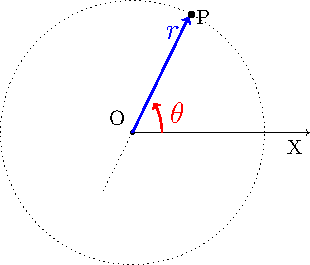
\includegraphics[width=5cm]{picture/vecter10.pdf}
 \caption{極座標系における座標の決定}
\label{fig:kyokuzahyou}
 \end{center}
\end{figure}

極座標系が直交直線座標系や斜交直線座標系とはちょっと趣の違った座標系であることが見て取れるだろう.
``座標''という用語を位置ベクトルを基底の線形結合で表したときの係数であると定義したが,
今回は基底とは独立に座標を定義している.
極座標系における基底はその座標をもとに定義されるのである.
このことに関しては後で話そうと思う.

そういえば,極座標系について説明するにあたり,$\theta$の範囲を制限したが,
実際にはそんなことをしない方がいろいろと便利である.
例えば,極座標系においての座標が$ \displaystyle \left(1, \, \frac{7}{4} \pi \right)$ となるような点と,
座標が$\displaystyle \left(1, \, - \frac{\pi}{4} \right)$となるような点は同じ点であるとみなすのである.
こうしてしまうと$r, \, \theta$の組と平面上の点が1対1に対応しなくなってしまう.
しかし,そんな細かいことは無視することにするのである.
こうすることで何がどのように便利になるかはけっこういろいろあるので自身で考えてみるといいだろう.

\begin{figure}[h]
 \begin{center}
 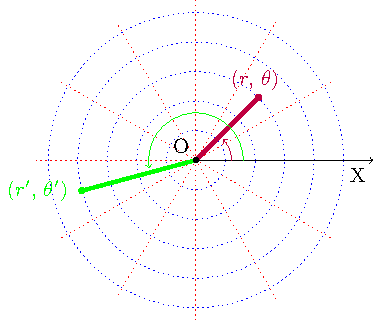
\includegraphics[width=6cm]{picture/vecter11.pdf}
 \caption{極座標系は直交曲線座標系である}
\label{fig:kyokukyokusen}
 \end{center}
\end{figure}

2次元のDescartes座標系においては,基準にしたのは2本の直交する直線であり,
斜交直線座標系においては,直交せず平行でない2本の直線であった.
では,極座標系においては何が基準になっているのだろう? 答えは図\ref{fig:kyokukyokusen}に
それとなく書いてあるのだが,それは円と直線である.
平面上に極を中心とする無数の円を描く.中心が決まっているのでそれらの円を特徴づけるのは半径である.
平面上に点が与えられたとき,その点と極との距離と同じ半径の円上にその点は存在していることになる.
つまり,点に与えられる座標のうち$r$の部分は,その点がどの円に属しているかを表すのである.
また,平面上に極を通る直線を無数に描く.通る点が1つ決まっているのでそれらの直線は
通る点をもう1つ決めることによって特徴づけることもできるが,違う特徴づけもできる.
それは,その直線とOXのなす角である.これは,ちょうど点の偏角$\theta$に相当しているのがわかるだろう.
すなわち,点に与えられる座標のうち偏角$\theta$に当たる部分は,
その点がどの直線に属しているかを表しているのである.

極座標系が極を通る直線と極を中心とする円を基準にしていることがわかるだろう.
そして,円と直線は互いにすべて直交している.
従って,極座標系は\emph{直交曲線座標系}\index[widx]{ざひょうけい@座標系!ちょっこうきょくせん@直交曲線---}
と呼ばれることもある.
しかし,直交曲線座標系が極座標系しかないというわけではない.
直交する曲線を用いるような座標系はすべて直交曲線座標系と呼ばれるからだ.
また,極座標系は曲線の中でも円を使っている.
そういうわけで,
2次元の極座標系は\emph{円座標系}\index[widx]{ざひょうけい@座標系!えん@円---|see{極座標系}}とも呼ばれる.
2次元のとわざわざ書いたのは,3次元だと違う呼ばれ方をするからだ.
そのことに関してはそのときに触れることにしよう.

さて,極座標系とDescartes座標系との関係を見てみよう.
結果から言うと,Descartes座標系での座標が$(x, \, y)$,
極座標系での座標が$(r, \, \theta)$であるような点において,
三角関数の定義により次の関係式が成り立っているといえる.
\begin{align}
\begin{aligned}
x & = r \cos \theta \\
y & = r \sin \theta 
\label{eq:kyokuhenkan}
\end{aligned}
\end{align}
もちろん,Descartes座標系での座標軸と始線と極をうまい具合にとらないと
こういうきれいな関係式は成り立たない.
具体的には,Descartes座標系での原点を極座標系での極とし,
Descartes座標系での$x$軸を極座標系での始線とするのである.
\begin{figure}[h]
 \begin{center}
 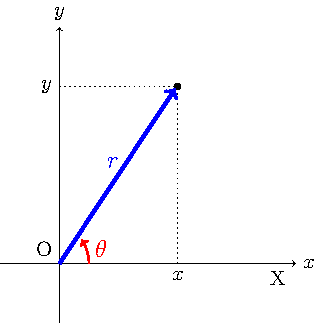
\includegraphics[width=5cm]{picture/vecter12.pdf}
 \caption{極座標系とDescartes座標系}
\label{fig:kyokuDescartes}
 \end{center}
\end{figure}

こうして見ると,極座標系における始線をOXと書いた理由がなんとなくわかる気がする.
始線OXと$x$軸が対応するようになっていたというわけだ.
原点と極,そして始線と$x$軸が一致しないようにして式(\ref{eq:kyokuhenkan})が破綻するように
することもできるのだが,この美しくわかりやすい関係式を捨てるという選択肢をとることはまずあるまい.
そういうわけで,極座標系を式(\ref{eq:kyokuhenkan})が成り立つような座標系というように定義している本はけっこう多い.
もちろんそれで間違っているわけではないのだが,極座標系というのはDescartes座標系
とはまったく独立に定義できるのだということ伝えたかったので,今回のような定義の仕方をしたのだった.

座標同士の関係式が終わったところで,いよいよ基底同士の関係式を求めてみよう.
斜交直線座標系での話を思い出してほしい.
それによれば,平面上の点について,
ある座標系における座標が$(x, \, y)$であり,別の座標系における座標が$(x', \, y')$
であるとき,それらの関係は行列$P$を用いて
\begin{align*}
\left[
\begin{array}{cc}
x' & y'
\end{array}
\right]
=
\left[
\begin{array}{cc}
x & y
\end{array}
\right]
{}^t \! P^{-1}
\end{align*}
というように表せるのであった.
いまはDescartes座標系と極座標系について考えているので
\begin{align*}
\left[
\begin{array}{cc}
r & \theta
\end{array}
\right]
=
\left[
\begin{array}{cc}
x & y
\end{array}
\right]
{}^t \! P^{-1}
\end{align*}
という関係式が成立するような行列$P$を探すことになる.
賢明な読者の方は気づいたはずだが,
そんな行列$P$はどう頑張っても見つからないのである.
なぜだろうか? 今までの議論のどこがに間違いがあったのだというのだろうか? 本当はこういうことについてじっくり悩むのは
とても有益なことなのだが,さっさと先に進んでしまいたいので結論を言ってしまおう.
すべての座標変換が行列を使って表せるわけではないのである.
行列を使って表せるような座標変換は\emph{線形変換}\index[widx]{せんけいへんかん@線形変換}と呼ばれ,
とても面白い性質を持った変換である.だが,性質のいい座標変換はこれだけではないのである.
斜交直線座標系は,たまたまDescartes座標系に
線形変換を施すことによって得られる座標系であったということだ.
だが今回は違うのである.違ったアプローチをする必要がありそうである.

そういえば,``極座標系における基底''とはいったいなんだろうか? Descartes座標系における基底は
標準基底のことで,斜交直線座標系における基底というのは引いた2本の直線と同じ向きのベクトルのことであった.
それに対して,``極座標系における基底''というのはいまいちイメージがつかない.
極座標系というのは円と直線を基準に据えているのであった.
これまでの話からすると,円と直線の向きに沿った2本のベクトルをとり,
それを極座標系における基底とするのだろう.
しかし,極座標系においては,直線といっても向きの違う直線が無数にあるし,
円の向きに沿ったベクトルなどという言葉は最早意味不明である.
意味不明なら定義してしまえばいい.よくわからない,
曖昧なものはきちんと定義して明確にしてしまえばいいのである.

とはいっても,どう定義したらいいだろうか.いままでの定義の方法は使えないが,
できれば同じような定義の方法を使いたいものである.
平面上において,ある1点Pを考える.極座標系においては点Pの座標は$(r, \, \theta)$であるとしておこう.
半直線OPの方向に大きさ1のベクトルをとり,これを$\bm{e}_r$とする.
そして,点Pが属している円の点Pにおける接線に平行な大きさ1のベクトルを
角度$\theta$を測った向きにとり,これを$\bm{e}_\theta$としておく.

各$r, \, \theta$について,$\bm{e}_r$と$\bm{e}_\theta$の長さは1で,しかも直交している.
もちろん,$ \{ \, \bm{e}_r, \, \bm{e}_\theta \, \} $は2次元平面$\mathbb{R}^2$の基底になっている. 
なんとなく標準基底と似ている気がするが,決定的に違う点が1つある.
それは,基底のとり方が座標に依存しているということだ.
いままでの座標系においては,基底は座標に依存することはなかった.
Descartes座標系においては標準基底$\bm{e}_x = 
\left[
\begin{array}{c}
1 \\
0
\end{array}
\right]
, \, 
\bm{e}_y =
\left[
\begin{array}{c}
0 \\
1
\end{array}
\right]$
であったし,斜交直線座標系においても定まった2本のベクトルをまず用意し,
それを使って平面上の点の位置を決めていたのであった.
しかし,いまとった基底に関しては,各点に対して1組ずつ基底が与えられており,
各点ごとにそれぞれの基底を用いるというイメージになっている.
\begin{figure}[h]
 \begin{center}
 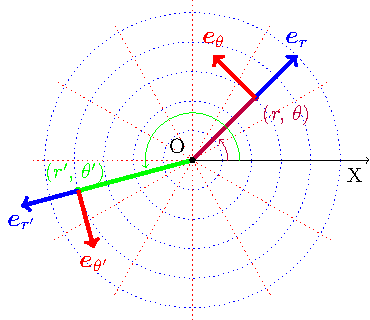
\includegraphics[width=6.5cm]{picture/vecter13.pdf}
 \caption{極座標系における基底のとり方}
\label{fig:kyokukitei}
 \end{center}
\end{figure}
\\
図\ref{fig:kyokukitei}において,
図中の点$(r, \, \theta)$と点$(r', \, \theta')$には違う基底が対応しているのが見て取れる.
しかし,$r$だけが変化してもそれに対応する基底は変化しない.
いまはわかりやすいように各点を始点にしてその点に対応する基底を描いているが,
平行移動して重なるようなベクトルは同じものとみなすからである.

ここまでやると,自分がこれからやろうとしていたことが少し変わっていることに気づく.
いままでは極座標系における定まった基底(そんなものはとれなかったが)と標準基底との関係を求めたかったのだが,
いまからやるのは極座標系において,点$(r, \, \theta)$に対応する基底$\{ \, \bm{e}_r, \, \bm{e}_\theta \, \} $と
標準基底との関係を求めることである.
ここまで引っ張ってしまって申し訳ないのだが,実はこの関係を求める作業は一瞬で終わってしまうのである.
結論だけ先に述べよう.
極座標系において,点$(r, \, \theta)$に対応する基底$\{ \, \bm{e}_r, \, \bm{e}_\theta \, \} $と
標準基底$\{ \, \bm{e}_x, \, \bm{e}_y \, \}$との関係は次の通りである.
\begin{align}
\begin{aligned}
\bm{e}_r& = & \cos \theta \, \bm{e}_x & & + \sin \theta \, \bm{e}_y & \\
\bm{e}_\theta & = &  - \sin \theta \, \bm{e}_x & & + \cos \theta \, \bm{e}_y &
\label{eq:kyokukiteihenkan}
\end{aligned}
\end{align}
わからない人は次の図\ref{fig:kyokukiteikankei}を3年ほどじっくり眺めてほしい.
\begin{figure}[h]
 \begin{center}
 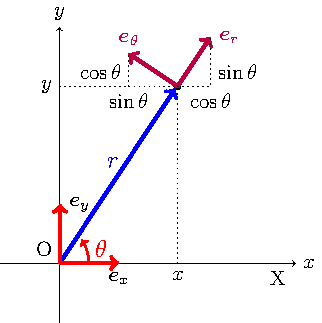
\includegraphics[width=5cm]{picture/vecter14.pdf}
 \caption{極座標系における基底と標準基底との関係}
\label{fig:kyokukiteikankei}
 \end{center}
\end{figure}
\\
これでもわからない人にヒントを出すと,$\bm{e}_r$というのは大きさが1だから,
図\ref{fig:kyokukiteikankei}を見ると,始点から大きさ$\cos \theta$だけ$\bm{e}_x$方向に進み,ついで
大きさ$\sin \theta$だけ$\bm{e}_y$方向に進むとちょうど$\bm{e}_r$の終点にたどり着くことになる.
これはつまり,$\bm{e}_r=\cos \theta \, \bm{e}_x + \sin \theta \, \bm{e}_y$が成り立つということである.
そうそう,もし``大きさ''と書いた量が負であれば,
それは``・・・方向に''というところを逆向きに進むのだと解釈してほしい.
面倒なので以後,こういった注釈は述べないことにする.

$\bm{e}_\theta$も同じように考えて,まず大きさ$\sin \theta$だけ$-\bm{e}_x$方向に進み,
さらにそこから大きさ$\cos \theta$だけ$\bm{e}_y$方向に進むことで$\bm{e}_\theta$の終点にたどり着くのである.
従って$\bm{e}_\theta = - \sin \theta \, \bm{e}_x + \cos \theta \, \bm{e}_y$が成り立つ.
ベクトルの和と三角関数の定義が頭に入っていればできてしまう簡単な作業である.
ここまであからさまなヒントを出せばできるだろう.式(\ref{eq:kyokukiteihenkan})において,
行列$P$を
\begin{align*}
P = \left[
\begin{array}{cc}
\cos \theta & -\sin \theta \\
\sin \theta & \cos \theta
\end{array}
\right]
\end{align*}
と定めれば,式(\ref{eq:kyokukiteihenkan})は
\begin{align*}
\left[
\begin{array}{cc}
\bm{e}_r & \bm{e}_\theta 
\end{array}
\right]
=
\left[
\begin{array}{cc}
\bm{e}_x & \bm{e}_y
\end{array}
\right]
P
\end{align*}
と書き換えられる.基底$\{ \, \bm{e}_x , \, \bm{e}_y \, \} $
から基底$\{ \, \bm{e}_r , \, \bm{e}_\theta \, \}$への変換行列はいま定義した$P$であるというわけだ. 

本当はもう少し伝えておきたいことはあるのだが,それはまた別の機会にして先に進むことにしよう.

\subsection{3次元空間における座標系}
これからやるのは3次元空間における座標系である.
よく3次元空間は``縦+横+高さ''と言われることがあるがそうではない.
これは,次元の概念を説明するときに触れたのだった.
とはいえ,このイメージはそこそこ役に立つものである.
ここでは,2次元平面での座標に対してさらにもう1個座標を追加することによって
3次元空間における座標系を構成してみよう.
\subsubsection{3次元直交直線座標系}\index[widx]{ざひょうけい@座標系!Descartes@Descartes---}
Descartes座標系から始めよう.
2次元のDescartes座標系では平面上に引かれた2本の直交する直線が基準であった.
3次元のDescartes座標系であれば,ここに直線を1本追加してやればいい.
直交直線座標系というだけあって,
加える直線はもともと引いてあった直線の両方に直線に直交するように引くことになる.

2次元のDescartes座標系においては,
平面に引かれた2本の直線はそれぞれ$x$軸,$y$軸と呼ばれるのであった.
そのつながりで,新たに引いた直線は\emph{$z$軸}と呼ばれるのが普通である.
$x$軸,$y$軸,$z$軸の3本の直線が空間内の座標を決定するルールの象徴になっている.
そういうわけで,Descartes座標系が導入された3次元空間は\emph{$xyz$空間}
と呼ばれることがある.
基底としては,3次元数ベクトル空間$\mathbb{R}^3$における
標準基底$\{ \, \bm{e}_1, \, \bm{e}_2, \, \bm{e}_3 \, \}$をそのまま持ってくればいい.
これらの標準基底は$xyz$空間の各軸に沿った大きさ1のベクトルになっている.
添え字を変えて$\{ \, \bm{e}_x, \, \bm{e}_y, \, \bm{e}_z \, \}$としておこう.

ところで,紙に$xyz$空間を描いてみると,
どうやら軸の引き方によって2種類の異なる座標系が出来上がるようなのだ.
\begin{figure}[h]
 \begin{minipage}{0.5\hsize}
  \begin{center}
   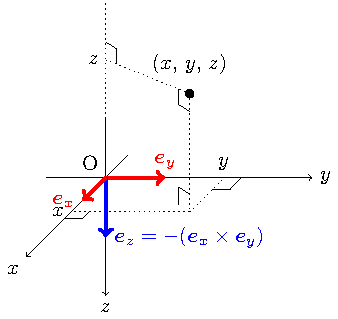
\includegraphics[width=5cm]{picture/vecter16}
  \end{center}
 \caption{左手系}
\label{fig:hidaritekei}
\end{minipage}
\begin{minipage}{0.5\hsize}
  \begin{center}
   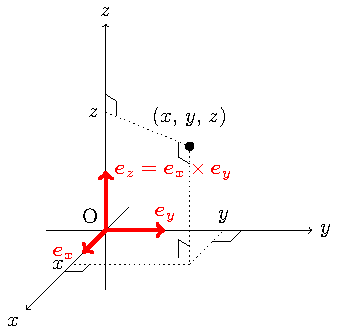
\includegraphics[width=5cm]{picture/vecter15}
  \end{center}
 \caption{右手系}
\label{fig:migitekei}
\end{minipage}
\end{figure}
\\
右と左に書いてある2つの座標系が違うのがわかるだろうか? 右(図\ref{fig:migitekei})に書いてある座標系は
\emph{右手系}\index[widx]{みぎてけい@右手系},
左(図\ref{fig:hidaritekei})に書いてある座標系は
\emph{左手系}\index[widx]{ひだりてけい@左手系}と呼ばれている.
右手系,左手系という言葉は本当はもう少し広い意味で使われているのだが,
ここでは省略させてもらうことにする.
両座標系を比較すると,$z$軸が逆向きに引かれているのがわかるだろう.
この2つの座標系はいくら回転させても重ね合わせることはできない.
ちょうど右手と左手の関係になっているというわけだ.

さて,普通Descartes座標系といえば図\ref{fig:migitekei}にある
右手系が業界標準である.
右手系においては$\bm{e}_z=\bm{e}_x \times \bm{e}_y$が成り立っているが,
左手系において成り立っているのは$\bm{e}_z = -( \bm{e}_x \times \bm{e}_y )$である.

演習として,次に示す4つの座標系がそれぞれ右手系であるか左手系であるか判定してみてほしい.
\begin{figure}[h]
 \begin{minipage}{0.5\hsize}
  \begin{center}
   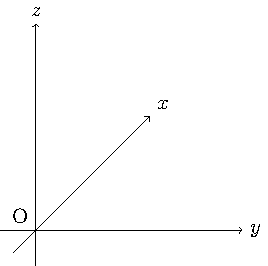
\includegraphics[width=3.5cm]{picture/vecter17}
  \end{center}
\end{minipage}
\begin{minipage}{0.5\hsize}
  \begin{center}
   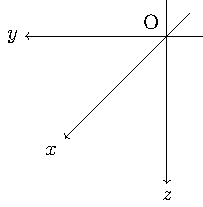
\includegraphics[width=3.5cm]{picture/vecter18}
  \end{center}
\end{minipage}
\end{figure}
\\
\begin{figure}[h]
 \begin{minipage}{0.5\hsize}
  \begin{center}
   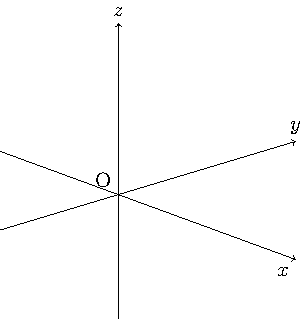
\includegraphics[width=3.7cm]{picture/vecter19}
  \end{center}
\end{minipage}
\begin{minipage}{0.5\hsize}
  \begin{center}
   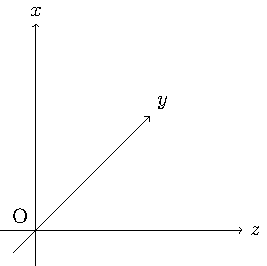
\includegraphics[width=3.5cm]{picture/vecter20}
  \end{center}
\end{minipage}
\end{figure}

\subsubsection{3次元斜交直線座標系}\index[widx]{ざひょうけい@座標系!しゃこうちょくせん@斜交直線---}
直交直線座標系の次は斜交直線座標系である.
といっても,Descartes座標系ほど語ることは多くはない.
さっさと進んでしまうことにしよう.

線形独立であるようなベクトルを3つとり,
これを$\mathbb{R}^3$の基底としてみる.
ここではそれを$\bm{a}, \, \bm{b}, \, \bm{c}$としてみよう.
ただし,これらのベクトルは直交しているわけではない.
大きさも1である必要はない.
この基底の取り方の自由さこそが斜交直線座標系の利点である.
$\bm{a}, \, \bm{b}, \, \bm{c}$の成分表示を
\begin{align*}
\bm{a} = \left[
\begin{array}{c}
a_x \\
a_y \\
a_z
\end{array}
\right]
\; , \;  \;
\bm{b} = \left[
\begin{array}{c}
b_x \\
b_y \\
b_z
\end{array}
\right]
\; , \;  \;
\bm{c} = \left[
\begin{array}{c}
c_x \\
c_y \\
c_z
\end{array}
\right]
\end{align*}
としてみる.
これらのベクトルは標準基底を用いて
\begin{align*}
\bm{a} & = a_x \bm{e}_x + a_y \bm{e}_y + a_z \bm{e}_z \\
\bm{b} & = b_x \bm{e}_x + b_y \bm{e}_y + b_z \bm{e}_z \\
\bm{c} & = c_x \bm{e}_x + c_y \bm{e}_y + c_z \bm{e}_z 
\end{align*}
と表せる.
よって,行列$P$を
\begin{align*}
P = \left[
\begin{array}{ccc}
a_x & b_x & c_x \\
a_y & b_y & c_y \\
a_z & b_z & c_z 
\end{array}
\right]
\end{align*}
と定めると,
\begin{align*}
\left[
\begin{array}{ccc}
\bm{a} & \bm{b} & \bm{c} 
\end{array}
\right]
= 
\left[
\begin{array}{ccc}
\bm{e}_x & \bm{e}_y & \bm{e}_z 
\end{array}
\right] P
\end{align*}
が成り立つ.ゆえに,標準基底$\{ \, \bm{e}_x , \, \bm{e}_y , \, \bm{e}_z \, \}$から
基底$\{ \, \bm{a} , \, \bm{b} , \, \bm{c} \, \}$への変換行列はこの$P$ということになる.
これは,以前も話した内容である.
\subsubsection{スカラー三重積とベクトル三重積}
書くことが少なくて寂しいのでちょっと寄り道をしてみよう.
$\bm{a}, \, \bm{b}, \, \bm{c}$の3本のベクトルの線形結合全体を考えると,
もちろんもとのベクトル空間である$\mathbb{R}^3$を再現する.
しかし,$\bm{a}, \, \bm{b}, \, \bm{c}$自体は,平行六面体を構成する.
これを``$\bm{a}, \, \bm{b}, \, \bm{c}$が張る平行六面体''と呼ぶことがある.
そして,その体積$V$は
\begin{align}
V = \bm{a} \cdot ( \bm{b} \times \bm{c} ) 
\label{eq:heikourokuV}
\end{align}
と表される.
このままだと$V$が負になることもあり,絶対値を付けておくべきである.
しかし式を簡単にするため,この$V$を符号付き体積とでも呼んでおくことにしよう.
\begin{figure}[h]
 \begin{center}
 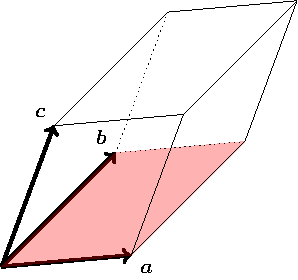
\includegraphics[width=4.5cm]{picture/vecter21.pdf}
 \caption{3つのベクトルが張る平行六面体}
\label{fig:heikourokumentai}
 \end{center}
\end{figure}
\\
図\ref{fig:heikourokumentai}中の色を付けた部分の面積が
$ \lvert \bm{a} \times \bm{b} \rvert $となることや
$ \bm{a} \cdot ( \bm{b} \times \bm{c} )$がスカラー量であることに納得がいき,
かつそれぞれの量が何を表しているかを考えられれば式(\ref{eq:heikourokuV})が
成り立つことは簡単に理解できるはずだ.
もしわからなければ,それは内積,外積の意味が理解できていないか,
もしくは平行六面体がどのような立体か理解していないだけである.
まぁその辺に関しては各自復習することにして,式(\ref{eq:heikourokuV})
を眺めながら,$V$のどこを底面とみなしているかを考えてやる.
そして,どこを底面とみるかを変えてやって,$V$を求めてやると,
次のような式が成り立つことがわかるはずだ.
\begin{align}
\bm{a} \cdot ( \bm{b} \times \bm{c} ) = \bm{c} \cdot ( \bm{a} \times \bm{b})
= \bm{b} \cdot ( \bm{c} \times \bm{a} ) 
\label{eq:sanjuuseki}
\end{align}
非常に対称的で美しい関係式である.
式(\ref{eq:sanjuuseki})中の \\
$\bm{a} \cdot ( \bm{b} \times \bm{c} ) , \, 
\bm{c} \cdot ( \bm{a} \times \bm{b}) , \, 
\bm{b} \cdot ( \bm{c} \times \bm{a} ) $
は$\bm{a}, \, \bm{b}, \, \bm{c}$の
\emph{スカラー三重積}\index[widx]{すからー@スカラー!さんじゅうせき@---三重積}と呼ばれている.
いまは線形独立である3つのベクトルについて考えたが,式(\ref{eq:sanjuuseki})は
$\bm{a}, \, \bm{b}, \, \bm{c}$が線形従属である場合にも成り立つ.
線形従属であるようなベクトル$\bm{a}, \, \bm{b}, \, \bm{c}$に対しては,
$\bm{a}, \, \bm{b}, \, \bm{c}$が張る平行六面体はつぶれてしまい,$V=0$になるからだ.
もうちょっと詳しくいうと,$\bm{a}, \, \bm{b}, \, \bm{c}$が線形従属のとき,
これらのベクトルは同一平面上にあって,$ \bm{b} \times \bm{c} $と$\bm{a}$が垂直になり,
その内積は0になる.他のパターンでも同じことが言えることはすぐにわかるはずだ.

スカラー三重積というからにはベクトル三重積というのもある.
3つのベクトル$\bm{a}, \, \bm{b}, \, \bm{c}$について,
新しいベクトル$ \bm{a} \times ( \bm{b} \times \bm{c} ) , \, ( \bm{a} \times \bm{b} ) \times \bm{c}$
を$\bm{a}, \, \bm{b} , \, \bm{c}$の
\emph{ベクトル三重積}\index[widx]{べくとる@ベクトル!さんじゅうせき@三重積}と呼ぶ.
ここまでまじめに学習してきた読者なら,なぜ私が
$ \bm{a} \times ( \bm{b} \times \bm{c} ) , \, ( \bm{a} \times \bm{b} ) \times \bm{c}$
とわざわざ2つ書いたかわかるはずだ.これら2つのベクトルは同じベクトルであるとは限らない.
ベクトル三重積についての詳細は省略するが,次のような等式が成立することが知られている.
\begin{align}
\begin{aligned}
\bm{a} \times ( \bm{b} \times \bm{c} ) = 
( \bm{a} \cdot \bm{c} ) \bm{b} 
- ( \bm{a} \cdot \bm{b} ) \bm{c} \\
\bm{b} \times ( \bm{c} \times \bm{a} ) = 
( \bm{b} \cdot \bm{a} ) \bm{c} 
- ( \bm{b} \cdot \bm{c} ) \bm{a} \\
\bm{c} \times ( \bm{a} \times \bm{b} ) = 
( \bm{c} \cdot \bm{b} ) \bm{a} 
- ( \bm{c} \cdot \bm{a} ) \bm{b} \\
( \bm{a} \times \bm{b} ) \times \bm{c}  = 
( \bm{a} \cdot \bm{c} ) \bm{b} 
- ( \bm{b} \cdot \bm{c} ) \bm{a} \\
( \bm{b} \times \bm{c} ) \times \bm{a}  = 
( \bm{b} \cdot \bm{a} ) \bm{c} 
- ( \bm{c} \cdot \bm{a} ) \bm{b} \\
( \bm{c} \times \bm{a} ) \times \bm{b}  = 
( \bm{c} \cdot \bm{b} ) \bm{a} 
- ( \bm{a} \cdot \bm{b} ) \bm{c} \\
\label{eq:vecsanjuuseki}
\end{aligned}
\end{align}
式の多さに圧倒されそうだが,実は式(\ref{eq:vecsanjuuseki})
のうちどれか1つでも覚えておけば残りの式はそこから導くことができる.
一番上の式
\begin{align*}
\bm{a} \times ( \bm{b} \times \bm{c} ) = 
( \bm{a} \cdot \bm{c} ) \bm{b} 
- ( \bm{a} \cdot \bm{b} ) \bm{c}
\end{align*}
の$\bm{a}$を$\bm{b}$に,$\bm{b}$を$\bm{c}$に
置き換えてみると,
\footnote{え? ``置き換える''の意味が分からないって? ならば$\bm{a}, \, \bm{b}, \, \bm{c}$を
○,×,△とでも``置き換えて''みよ.}
2番目の式
\begin{align*}
\bm{b} \times ( \bm{a} \times \bm{b} ) = 
( \bm{b} \cdot \bm{a} ) \bm{c} 
- ( \bm{b} \cdot \bm{c} ) \bm{a}
\end{align*}
が導けるし,一番上の式と4番目の式を比較すると,これはちょうどかける順番が逆になっている.
外積においてかける順番を逆にするとどうなるかは以前話した通りである.
そんなこんなで同じようにしていけば残りの式も導くことができる.
まぁこの式をどこで使うかといわれると正直微妙なところはあるが.
式(\ref{eq:vecsanjuuseki})をよくよく眺めていると,
\begin{align}
\begin{aligned}
\bm{a} \times ( \bm{b} \times \bm{c} ) + \bm{b} \times ( \bm{c} \times \bm{a} ) + 
\bm{c} \times ( \bm{a} \times \bm{b} ) = \bm{0} \\
( \bm{a} \times  \bm{b} ) \times \bm{c} + ( \bm{b} \times  \bm{c} ) \times \bm{a} +
( \bm{c} \times  \bm{a} ) \times \bm{b} = \bm{0}
\label{eq:Jacobi}
\end{aligned}
\end{align}
という等式が成り立っていることに気が付くはずだ.
式(\ref{eq:Jacobi})は\textbf{Jacobiの恒等式}\index[widx]{Jacobiのこうとうしき@Jacobiの恒等式}
\index[nidx]{Jacobi@Jacobi(ヤコビ)}
と呼ばれているものの一部である.
一部というからには一般のものがあるわけなのだが,ちょっと説明がややこしいので省略させてもらおう.

ところで,3次元Descartes座標系のところで右手系と左手系というのが出てきたが,
スカラー三重積の知識があると,右手系,左手系という概念をもう少し一般に定義することができる.

3次元空間$\mathbb{R}^3$の基底を1組とり,これを$\Set{ \bm{a} , \, \bm{b} , \, \bm{c} }$
とする.$\bm{a} , \, \bm{b} , \, \bm{c}$
のスカラー三重積$\bm{a} \cdot ( \bm{b} \times \bm{c} )$
が正の値をとるとき,基底$\Set{ \bm{a} , \, \bm{b} , \, \bm{c} }$
は$\mathbb{R}^3$の\emph{右手系}\index[widx]{みぎてけい@右手系}をなすといい,
$\bm{a} \cdot ( \bm{b} \times \bm{c} )$
が負の値をとるとき,基底$\Set{ \bm{a} , \, \bm{b} , \, \bm{c} }$
は$\mathbb{R}^3$の\emph{左手系}\index[widx]{ひだりてけい@左手系}をなすという.

ぴったり直交しているわけではなくとも,
基底同士の向きの関係がDescartes座標系のときと
おおよそ同じようなものであればそれらを全部右手系とみなすのである.
Descartes座標系における標準基底$\Set{ \bm{e}_x , \, \bm{e}_y, \, \bm{e}_z }$
はもちろん$\mathbb{R}^3$の右手系をなしている.
これから学ぶ極座標系の基底もやはり$\mathbb{R}^3$の右手系をなす.
座標系は右手系を用いるのが業界標準なのである.

\subsubsection{3次元極座標系}\index[widx]{ざひょうけい@座標系!きょく@極---}
さて,お次は極座標系である.
極座標系においては基底ベクトルを増やしていくというアプローチは通用しない.
2次元極座標系においては,基底の代わりに幾何学的に座標を決定するルールを与えたのだった.
今回もその方法を利用していくことにする.

2次元極座標系のときに座標を決定するために用いたのは,
極を中心とする無数の円とそれに直交するような極を通る無数の直線であった.
3次元空間での点の座標を決定するには,ここにもうひとつ新たな要素を付け加えてやればいい.
ここでは,もうひとつ円を追加してやることにする.
この円は,極が中心で
かつ2次元極座標系のときの円と直線が存在した平面からは飛び出していることにしよう.
さらに,この円はもとの平面と直交しているという条件も付け加えてやる.
ここまで厳しい条件を付け加えないと使いやすい座標系は出来上がらないのだ.
もうひとつ円を追加すると書いたが,実際には上に書いたような条件をみたすような
円を無数に描くのだ.円の半径は特に指定してはいなかった.

2次元極座標系において,平面上の点が円上のどこにあるかを決定するのに,
始線とその点の動径のなす角を用いたのであった.
今回は円を追加したのだから,始線を追加してやればなんとかなりそうだ.
その始線をOZとしてみよう.空間内に点Zをとり,半直線OZを始線とするのである.
ただし,OZはOXと垂直であるということにしておく.

極と2本の始線によって,空間内の点の座標を定めよう.
我々に与えられたのは,極Oと直交する2本の半直線OX,OZである.
空間内に点Pがあったとする.まず2点O,Pの距離を求め,これを$r$とする.
次に,直線OPと半直線OZのなす角をはかり,これを$\theta$とおく.
そして,極Oを通り,OZに垂直な平面を考え,
極Oと,点Pからその平面に降ろした垂線の足の2点を通る直線を引く.
その直線と半直線OXのなす角を$\varphi$とする.
少し長くなったが,頭の中にイメージが思い浮かぶだろうか? 下の図と
自分が抱いていたイメージがおおむね一致するかをチェックしてほしい.
\begin{figure}[h]
 \begin{center}
 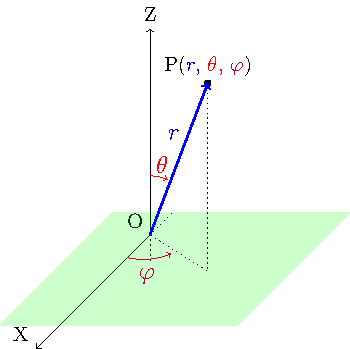
\includegraphics[width=5.7cm]{picture/vecter22.pdf}
 \caption{3次元極座標系における座標の決定}
\label{fig:3dkyokuzahyou}
 \end{center}
\end{figure}

空間内に与えられた点Pに対し,Pが直線OZ上になければ,$ r, \, \theta, \, \varphi $は必ず求めることができる.
そして,$r>0, 0 \leq \theta \leq \pi , \, - \pi < \varphi \leq \pi$とでもしておけば,
直線OZ上の点を除いては,各$r, \, \theta, \, \varphi$に対してそれに対応する点がただひとつ定まる.
そのとき,その点の座標は$(r, \, \theta, \, \varphi)$であると定義する.
直線OZ上の点に対しては$\varphi$を求めることができず,さらに極Oに関しては$\theta$も求めることができない.
だが,2次元極座標系のときと同じようにそんな細かいことは考えないことにする.
とにかく,これで空間内にある点の座標を定めるルールが決まったことになり,
無事に3次元極極座標系が定義されたことになる.

3次元極座標系における座標の決定は,極を通る無数の直線と,極を中心とする無数の円
によってなされるのであった.この円は,あらゆる方向に描かれている.
空間に点が与えられたとき,$r$がその点が属する円の半径を決め,
与えられた点が属する円がどの方向を向いた円かを$\varphi$が決定し,
$\theta$によってその円のどこに点が存在するかが決定されるのである.
しかし,あらゆる方向を向いた円が無数に存在している状況は,
その円と同じ半径の球が1つ存在している状況とまったく同じである.
円をその中心を通る軸周りに1回転して得られる
図形が球であることを思い出せば容易に納得できるだろう.
従って,3次元極座標系における座標の決定は,
極を通る無数の直線と,極を中心とする無数の球によってなされると考えることができるのである.
このイメージにおいては,空間に点が与えられたとき,まず$r$がその点が属する球の半径を決め,
その球のどこに点があるかを$\varphi, \, \theta$が決定するということになる.
この考え方でも座標の決定には何ら問題はなさそうである.
このことから,3次元極座標系は\emph{球面座標系}\index[widx]{ざひょうけい@座標系!きゅうめん@球面---},
もしくは\emph{球座標系}と呼ばれることがある.
なかなかよくできたネーミングである.

さて,ここからは3次元極座標系と3次元Descartes座標系との関係について考えてみる.
まずは座標同士の関係式だが,もはや何も言うまい.Descartes座標系における座標が
$(x, \, y, \, z)$であり,極座標系における座標が$(r, \, \theta, \, \varphi)$であるような点について,
以下のような関係式が成り立っている.
\begin{align}
\begin{aligned}
x & = r \sin \theta \cos \varphi \\
y & = r \sin \theta \sin \varphi \\
z & = r \cos \theta
\label{eq:kyokuDechenkan}
\end{aligned}
\end{align}
もちろん,これは式(\ref{eq:kyokuDechenkan})のような美しい関係式を得るために
極や始線の取り方を工夫した結果である. 
具体的には図\ref{fig:kyokuDeckankei}のように,極座標系における極OをDescartes
座標系における原点Oと一致させ,さらに極座標系における始線OX,OZをそれぞれ
Descartes座標系における$x$軸,$z$軸と一致させたのである.
\begin{figure}[h]
 \begin{center}
 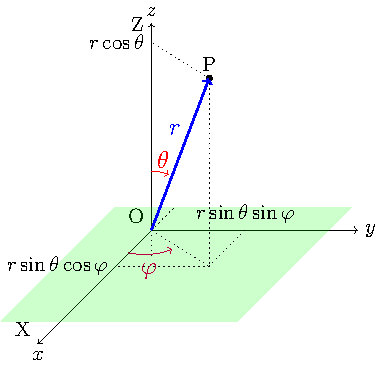
\includegraphics[width=6.2cm]{picture/vecter23.pdf}
 \caption{極座標系とDescartes座標系}
\label{fig:kyokuDeckankei}
 \end{center}
\end{figure}
\\
もし式(\ref{eq:kyokuDechenkan})に納得できないときは,
$\theta$がどんな角度だったかを思い出してほしい.
そうすればおそらく納得できるはずだ.
$\theta$がどんな角であるかを思い出せればPから$xy$平面に降ろした垂線の足と
原点との距離が$r \sin \theta$であることがわかる.
それさえわかればあとは自分でできるだろう.

さて,ここから基底同士の関係について考えてみよう.
そのためには,まず3次元極座標系における基底を定義しなくてはならない.

極座標系における座標が$(r, \, \theta, \, \phi)$であるような点Pについて考える.
OからPに向かう方向に長さ1のベクトルをとり,これを$\bm{e}_r$とする.
次に,極Oを中心とし,点Pを通り,かつ2直線OP,OZが張る平面に含まれるような円を考え,
その円の点Pにおける接線に平行な大きさ1のベクトルを$\theta$を測った向きにとり,
これを$\bm{e}_\theta$とする.
最後に,極Oを通り,$\bm{e}_\theta$に垂直な平面上に極Oを中心としてOPを半径とする円を考え,
その円の点Pにおける接線に平行な大きさ1のベクトルを$\varphi$を測った向きにとり,
これを$\bm{e}_\varphi$とする.
\begin{figure}[h]
 \begin{center}
 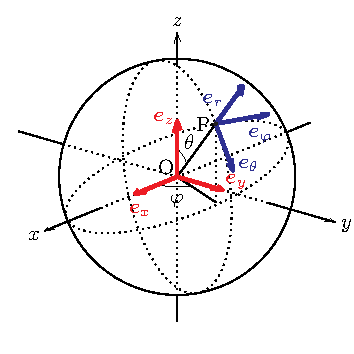
\includegraphics[width=7cm]{picture/vecter30.pdf}
 \caption{3次元極座標系における基底}
\label{fig:3dkyokukitei}
 \end{center}
\end{figure} \\
文章を読んで頭に思い浮かんだ図と図\ref{fig:3dkyokukitei}が一致するだろうか.
図\ref{fig:3dkyokukitei}から,$\bm{e}_r, \, \bm{e}_\theta, \, \bm{e}_\varphi$を
$\bm{e}_x, \, \bm{e}_y, \, \bm{e}_z$で表せば
\begin{align}
\begin{aligned}
\bm{e}_r & = & \sin \theta \cos \varphi \, \bm{e}_x & & + \sin \theta \sin \varphi \, \bm{e}_y &
& + \cos \theta \, \bm{e}_z & \\
\bm{e}_\theta & = & \cos \theta \cos \varphi \, \bm{e}_x & & + \cos \theta \sin \varphi \, \bm{e}_y & 
& -  \sin \theta \,  \bm{e}_z & \\
\bm{e}_\varphi & = & - \sin \varphi \, \bm{e}_x & & + \cos \varphi \, \bm{e}_y &
\label{eq:kyokuDeckitei}
\end{aligned}
\end{align}
となることがわかる.わかるといって理解できれば苦労しないので,
式(\ref{eq:kyokuDeckitei})に関しては少しばかり解説を入れておこう.
といっても,やることは2次元のときとそれほど大きく変わるわけではない.

$\bm{e}_r$について考える.図中の点P($r, \, \theta , \, \varphi$)と同じ方向に大きさ1だけ進むことを考えればよい.
簡単のため,$\bm{e}_r$の始点は極Oにあるとしておこう.
こういうことを考えるとき,3次元空間をある平面に正射影した図というのは非常に役に立つ.
正射影というと偉そうに聞こえるが,要は上から見るとか横から見るとかそういうことである.
\footnote{空間に存在する図形$S$と平面$\pi$について,$S$から$\pi$に降ろした垂線の足全体の集合を
$S$の$\pi$への正射影と呼ぶ.また,$S$の$\pi$への正射影を考えることを
$S$を$\pi$に正射影するという.}\index[widx]{せいしゃえい@正射影|textbf}
\begin{figure}[h]
 \begin{minipage}{0.5\hsize}
  \begin{center}
   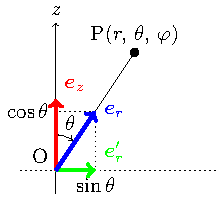
\includegraphics[width=5cm]{picture/vecter24}
  \end{center}
 \caption{3次元空間の直線OPと$z$軸を含む平面への正射影}
 \label{fig:z-OP}
\end{minipage}
\begin{minipage}{0.5\hsize}
  \begin{center}
   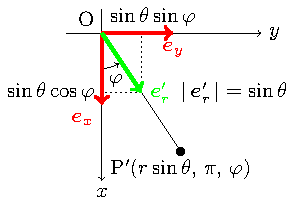
\includegraphics[width=6cm]{picture/vecter25}
  \end{center}
 \caption{3次元空間の$xy$平面への正射影}
 \label{fig:3dxy}
\end{minipage}
\end{figure} \\
まず,図\ref{fig:z-OP}を見てほしい.この図は3次元空間を直線OPと$z$軸を含む平面に正射影した図である.
$\bm{e}_r$はこの平面に含まれるベクトルである.
$\bm{e}_r$を$\bm{e}_z$と$\bm{e}_z$に垂直で,その終点が$\bm{e}_r$の終点から極Oを通り,
$z$軸に垂直な直線に降ろした垂線の足に一致するようなベクトル$\bm{e}'_r$とに分解する.
三角関数の定義から,$\bm{e}_r = \cos \theta \, \bm{e}_z + \bm{e}'_r $
が成り立つことはすぐにわかる.そして,$| \, \bm{e}'_r \, | = \sin \theta$が成り立つこともわかる.
そして,$\bm{e}'_r$は$xy$平面に含まれるベクトルなので,
$\bm{e}'_r$は$\bm{e}_x, \, \bm{e}_y$を用いて表せるはずだ.
そこで,3次元空間を$xy$平面に正射影したのが図\ref{fig:3dxy}である.
$\bm{e}_r$を$xy$平面に正射影すると$\bm{e}'_r$が得られる.
$\bm{e}'_r$の大きさは$\sin \theta$であり,従って$\bm{e}'_r$の始点を極Oに固定し,
極Oと$\bm{e}'_r$の終点から$x$軸に降ろした垂線の足までの距離は$\sin \theta \cos \varphi$となり,
そして極Oと$\bm{e}'_r$の終点から
$y$軸に降ろした垂線の足までの距離は$\sin \theta \sin \varphi$となる.
以上の考察により,$\bm{e}'_r = \sin \theta \cos \varphi \, \bm{e}_x 
+ \sin \theta \sin \varphi \, \bm{e}_y$が成り立ち,
従って$\bm{e}_r = \sin \theta \cos \varphi \, \bm{e}_x + \sin \theta \sin \varphi \, \bm{e}_y 
+ \cos \theta \, \bm{e}_z$が成り立つことがわかる.

次に,$\bm{e}_\theta$について考えよう.
これも正射影した図を見ながら考えることにする.
\begin{figure}[h]
 \begin{minipage}{0.5\hsize}
  \begin{center}
   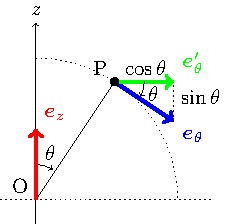
\includegraphics[width=4cm]{picture/vecter26}
  \end{center}
 \caption{3次元空間の直線OPと$z$軸を含む平面への正射影}
 \label{fig:z-OP-theta}
\end{minipage}
\begin{minipage}{0.5\hsize}
  \begin{center}
   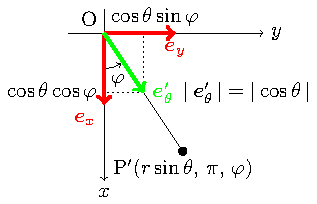
\includegraphics[width=6cm]{picture/vecter27}
  \end{center}
 \caption{3次元空間の$xy$平面への正射影}
 \label{fig:3dxy-theta}
\end{minipage}
\end{figure} \\
まず見るべきは図\ref{fig:z-OP-theta}である.
この図は3次元空間を直線OPと$z$軸を含む平面に正射影した図である.
$\bm{e}_r$のときと同じように$\bm{e}_\theta$もこの平面に含まれるベクトルである.
$\bm{e}_\theta$の始点を点Pに固定し,点Pを始点とし,$\bm{e}_\theta$の終点から
点Pを通り,$z$軸に垂直な直線に降ろした垂線の足を終点とするようなベクトルを$\bm{e}'_\theta$とする.
すると$\bm{e}_\theta$と$\bm{e}'_\theta$のなす角は$\theta$である.
このことは中学生でもわかることであるから省略させてもらおう.
このことから,$| \, \bm{e}'_\theta \, | = | \cos \theta \, |$となり,
\footnote{$\sin \theta$は$- \pi < \theta \leq \pi $の範囲では負にはならないが,
$\cos \theta$はそうはいかないので絶対値をつけている.
これ以外の``大きさ''や``距離''に関してはそういう配慮はしていない.}
$\bm{e}_\theta$は$\bm{e}_\theta = - \sin \bm{e}_z + \bm{e}'_\theta$と表せることがわかる.
$\bm{e}'_\theta$は$\bm{e}_r$のときと同じように考えて,図\ref{fig:3dxy-theta}から
$\bm{e}'_\theta = \cos \theta \cos \varphi \, \bm{e}_x + \cos \theta \sin \varphi \, \bm{e}_y$
と表せる.$| \, \bm{e}'_\theta \, | = | \cos \theta \, |$である以外はさっきとまったく同じである.
以上の考察の末,$\bm{e}_\theta = \cos \theta \cos \varphi \, \bm{e}_x 
+ \cos \theta \sin \varphi \, \bm{e}_y - \sin \theta \, \bm{e}_z$と表せることがわかる.
少しばかりややこしいが決して難しいというわけでもない.

最後に残るは$\bm{e}_\varphi$である.(始点を$xy$平面のどこかにしてみれば)
$\bm{e}_\varphi$は$xy$平面に含まれるベクトルなので,
$\bm{e}_x$と$\bm{e}_y$のみで表せるはずである.
よって,3次元空間を$xy$平面に正射影すると,それは図\ref{fig:3dxy-varphi}のようになる.
\begin{figure}[h]
 \begin{center}
 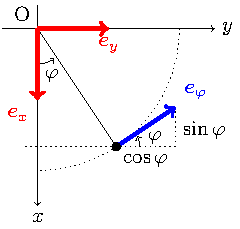
\includegraphics[width=4cm]{picture/vecter28.pdf}
 \caption{3次元空間の$xy$への正射影}
\label{fig:3dxy-varphi}
 \end{center}
\end{figure}
\\
$\bm{e}_\varphi$は原点を中心とし,OPを半径とする円の点Pにおける接線に平行なのであった.
図\ref{fig:3dxy-varphi}では,この円を回転し,さらに$\bm{e}_\varphi$を平行移動させて,
この円が$xy$平面上にあり,かつ$\bm{e}_\varphi$の始点が回転後の円の点Pに相当する点になるようにしてある.
$\bm{e}_\varphi$がOPと垂直であることや$\bm{e}_\varphi$を$\varphi$を測った向きに取ったことを加味すれば,
$\bm{e}_\varphi$と,$\bm{e}_\varphi$の始点を通って$y$軸に平行な直線のなす角は$\varphi$になり,
あとは$\bm{e}_r$や$\bm{e}_\theta$のときと同様に考えて
$\bm{e}_\varphi= - \sin \varphi \, \bm{e}_x + \cos \varphi \, \bm{e}_y$
となることがわかる.

以上で式(\ref{eq:kyokuDeckitei})は理解できたことになる.
実はもっと簡単にこの式を導く方法があるのだが,
それはまた後にしておこう.

なお,この基底$\Set{ \bm{e}_r , \, \bm{e}_\theta , \, \bm{e}_\varphi}$は
基底を構成するベクトルが互いに直交し,かつすべてのベクトルの大きさが1である.
このことは図からも明らかであるし,式(\ref{eq:kyokuDeckitei})
を用いて直接計算することもできる.
いちいち解説する必要もないだろう.

\subsubsection{円筒座標系}
3次元極座標系において,2次元極座標系を3次元極座標系に拡張するために用いたのは
新たに追加した始線と動径のなす角であった.
ここでは,別のアプローチをしてみよう.

極Oと始線OXをとり,さらに極Oを通ってOXに垂直な半直線を引く.
ここまでは3次元極座標系のときと同じであるが,
ここではこの直線に$z$軸という名前を付けよう.
そして,空間にある点Pに対し,Pと$z$軸との距離を$r$,
Pから$z$軸に降ろした垂線の足から極Oまでの(向き付きの)距離を$z$,
さらに,極Oを通ってOZに垂直な平面を考え,
極Oと,点Pからその平面に降ろした垂線の足の2点を通る直線を引く.
その直線と半直線OXのなす角を$\theta$とする.
これを図示してみれば,図\ref{fig:entou}のようになる.
\begin{figure}[h]
 \begin{center}
 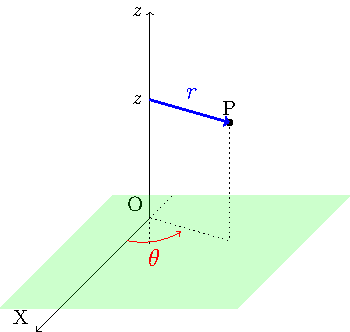
\includegraphics[width=5.2cm]{picture/vecter29.pdf}
 \caption{円筒座標系における座標の決定}
\label{fig:entou}
 \end{center}
\end{figure}


この$r, \, \theta, \, z$に対し,点Pの座標は$(r, \, \theta, \, z)$であると定めるのである.
極座標系のときと同じように,$z$軸上の点に対しては$\theta$の値を定めることはできないが,
やはりそういう細かいことは考えないことにする.
とにかく,こうして3次元空間にある点の座標を決定する規則,
すなわち座標系が導入できたわけである.

この座標系は,$z$軸の各点を中心とする無数の円が存在して,
$r$と$z$によって空間にある点がどの点にあるかを決定され,
$\theta$が点がその円上のどこにあるかを決定するようなイメージである.
$r$を固定して$z$と$\theta$を動かしてみれば,その軌跡は無限に長く伸びる円柱になる.
このことから,いま導入した座標系は
\emph{円筒座標系}\index[widx]{ざひょうけい@座標系!えんとう@円筒---}と呼ばれている.

さて,円筒座標系とDescartes座標系の関係について考える.
Descartes座標系における原点Oが円筒座標系における極Oに一致し,
さらにDescartes座標系における$x$軸,$y$軸が
それぞれ円筒座標系における半直線OXと$z$軸に一致するとしよう.
円筒座標系においてその座標が$(r, \, \theta, \, z)$であり,Descartes座標系における
座標が$(x, \, y, \, z)$であるような点において,以下に示すような関係式が成り立っている.
\begin{align}
\begin{aligned}
x & = r \cos \theta \\
y & = r \sin \theta \\
z & = z
\label{eq:entouDeczahyou}
\end{aligned}
\end{align}
式(\ref{eq:entouDeczahyou})に関してはもはや解説はいらないだろう.
2次元極座標系のときとまったく同様に考えておけばよい.

基底に関しても同様である.円筒座標系における座標が$(r, \, \theta, \, z)$であるような点Pにおいて,
半直線OPと同じ方向に大きさ1のベクトルをとり,これを$\bm{e}_r$とする.
さらに,Pから$z$軸に降ろした垂線の足を中心とし,半径$r$の円を考え,その円のPにおける接線に平行な
大きさが1のベクトルを$\theta$を測った向きにとり,これを$\bm{e}_\theta$とする.
最後に$z$軸と同じ向きに大きさ1のベクトルをとり,これを$\bm{e}_z$としておこう.
わざわざ図示しなくてもイメージできるはずだ.円筒座標系における基底は2次元極座標系のときの基底に
$\bm{e}_z$が生えたような様子になっている.
Descartes座標系での基底,つまり標準基底$\{ \, \bm{e}_x, \, \bm{e}_y, \, \bm{e}_z \, \} $との関係は
\begin{align}
\begin{aligned}
\bm{e}_r& = & \cos \theta \, \bm{e}_x & & + \sin \theta \, \bm{e}_y & \\
\bm{e}_\theta & = &  - \sin \theta \, \bm{e}_x & & + \cos \theta \, \bm{e}_y & \\
\bm{e}_z & = & & & & \; \; \; \;\;\;\; \bm{e}_z
\label{eq:entoukiteihenkan}
\end{aligned}
\end{align}
となる.この基底$\Set{ \bm{e}_r , \, \bm{e}_\theta , \, \bm{e}_z}$
を構成するベクトルは互いに直交するベクトルであり,かつすべてのベクトルの大きさが1である.
これも2次元極座標系のときとほとんど変わらない.
 % ベクトル
\chapter{ベクトル解析}
微分積分を用いて関数の性質を調べる学問を\emph{解析学}という.
なのでベクトル解析といえば,微分積分を使ってベクトルの性質を調べる学問である.
だがその前に,解析の対象となる場について確認しておこう.

\section{ベクトル場とスカラー場}
\subsection{ベクトル値関数}
空間に何かが存在している状態を考える.
その``何か''が具体的に何であるかは問わない.
しかし,その何かは空間のある特定の位置を決めれば,
その何かを象徴するようなベクトルやスカラーといった量を得ることができるとする.
例えば空間の温度分布を考えると,
位置を決めると温度$T$というスカラー量が得られる.
空間の風の分布を考えてみれば,
位置を決めたときに得られるのは風の向きと強さ$\bm{v}$であり,
これはベクトル量と解釈するのがよいだろう.

上の2つの例を見ると,重要なのは
位置とスカラー量,それに位置とベクトル量の対応関係
であることが見て取れる.
スカラー量だけでもベクトル量だけでもいけない.
それらと位置との対応関係が重要なのである.
位置とスカラー量の対応関係というのはそのまま多変数関数のことである.
3変数関数だと思えばよい.
しかし,位置とベクトル量の対応関係はそのまま多変数関数とみなすことはできない.
位置というのは本質的にはベクトル量のことであるから,
位置とベクトル量の対応関係というのはベクトル量とベクトル量の対応関係のことである.
\pageref{eq:nhensu}ページにある関数の定義を見てみると,
関数というのは数(の組)と数の対応関係のことであると書いてある.
数の組というのは数ベクトルと同一視できるから,
関数というのはベクトル量とスカラー量の対応関係のことであるといえる.
しかし,ベクトル量とスカラー量の対応関係もベクトル量とベクトル量の
対応関係も似たようなものである.
あえて両者を区別する必要もあるまい.
そこで,とる値,すなわち従属変数がベクトル量であるような関数のことを
\emph{ベクトル値関数}\index[widx]{べくとるちかんすう@ベクトル値関数}と呼ぶことにしよう.
\footnote{ベクトル値関数という用語があるからにはスカラー値関数という用語もあってよさそうだが,
普通の多変数関数と何も変わらないのでスカラー値関数という用語が使われることはあまり多くはない.}
書籍によってはベクトル値関数を多変数関数と呼んでいる場合がある.
数(の組)と数(の組)の対応関係が関数であるとしているのである.
こうしたところでまったく不都合はないし,むしろこっちの方が便利な気がする.
このあたりのことは流儀によってだいぶ違うので,
違う本を読むときには混乱しないように気を付けよう.

\subsection{場とは位置の関数である}
多変数関数やベクトル値関数のなかで,独立変数(の組)が位置であるような状況を考える.
独立変数が$x, \, y, \, z$の3つであってもいいし,これを1つのベクトルとみなして$\bm{r}$と表してもいい.
そのイメージは,空間にスカラー量やベクトル量が存在し,
位置を決めたときにそこにあるスカラー量やベクトル量を取り出してくるようなものである.
位置に対してスカラー量を対応させるような関数を\emph{スカラー場},\index[widx]{すからーば@スカラー場}
ベクトル量を対応させるような関数を\emph{ベクトル場}\index[widx]{べくとるば@ベクトル場}と呼ぶ.
それに対し,周波数やエネルギーにスカラー量やベクトル量を対応させるような関数を
\emph{スペクトル}\index[widx]{すぺくとる@スペクトル}と呼ぶ.
なんだか抽象的に見えるが,スカラー場やベクトル場は常日頃から付き合っている概念である.
その証拠に次の図\ref{fig:ondo}と図\ref{fig:husoku}を見てほしい.

\begin{figure}[h]
 \begin{minipage}{0.5\hsize}
  \begin{center}
   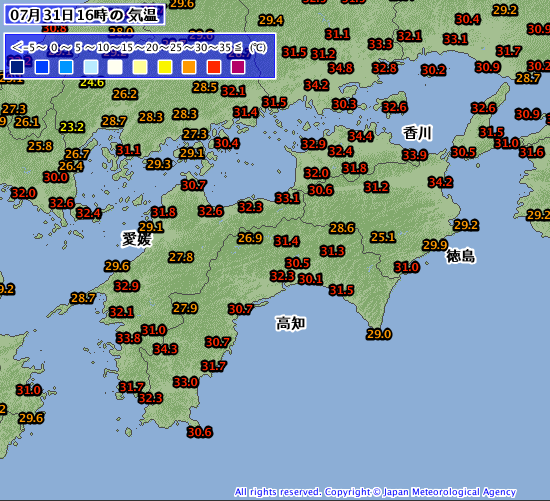
\includegraphics[width=5.5cm]{picture/vecterana1}
  \end{center}
 \caption{高知県周辺の気温(気象庁ホームページより)}
 \label{fig:ondo}
\end{minipage}
\begin{minipage}{0.5\hsize}
  \begin{center}
   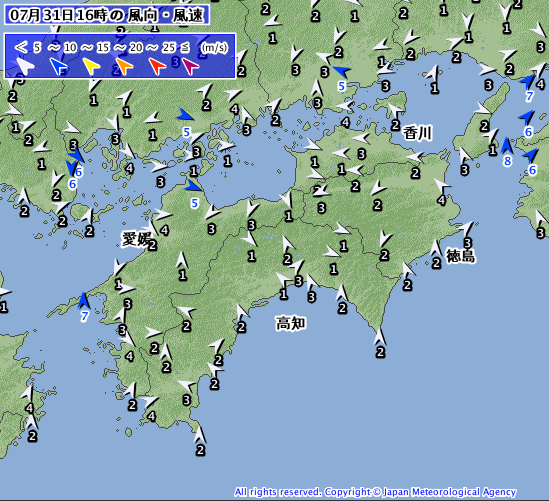
\includegraphics[width=5.5cm]{picture/vecterana2}
  \end{center}
 \caption{高知県周辺の風向と風速(気象庁ホームページより)}
 \label{fig:husoku}
\end{minipage}
\end{figure} 
ちょっと小さくて図が見えにくいかもしれないが,
天気予報とかでよく出てくる図である.
図\ref{fig:ondo}が位置に対してそこの気温というスカラー量
が決まっているような対応関係を表している図であり,
図\ref{fig:husoku}が位置に対して風向と風速というベクトル量が
決まっているような対応関係を表している図である.
すなわち,図\ref{fig:ondo}がスカラー場,図\ref{fig:husoku}が
ベクトル場を表しているような図であるというわけだ.
本来ベクトルの大きさというのは,矢印の長さで表すのが普通であるが,
図\ref{fig:husoku}は風速を矢印の色で表している.
数学や物理学のルールはその分野でもっとも便利になるように作られているので,
それ以外ではそのルールに従う必要はないのである.

ちょっと話が長くなったが,これからやるのはベクトル場やスカラー場を微分積分学の手法を用いて調べていくことである.

\section{ベクトルの微分}
まずは微分からやってみよう.$n$次元の数ベクトル$\bm{A}$があるスカラー量$t$の関数$\bm{A}(t)$だったとする.
これはつまり,$\bm{A}(t)$の各成分が$t$の関数であるということである.
\begin{eqnarray}
\bm{A}(t) = \left[
\begin{array}{c}
 A_1 (t) \\
 A_2 (t) \\
 \vdots \\
 A_n (t)
 \end{array}
\right]
\label{eq:vect}
\end{eqnarray}

$t$が微小量$\mathrm{d}t$だけ変化したとき,$\bm{A}(t)$がどれだけ変化をするかを求めたい.
微分法を使う動機はそのようなものだった.
$\bm{A}(t)$の変化$\mathrm{d} \bm{A}(t)$は
$$
\mathrm{d} \bm{A}(t) = \bm{A} (t+ \mathrm{d} t) - \bm{A} (t)
$$
である.成分表示すれば
\begin{eqnarray*}
\mathrm{d} \bm{A}(t) & = &\bm{A} (t+ \mathrm{d} t) - \bm{A} (t) \\
& = & \left[
\begin{array}{c}
A_1 (t+ \mathrm{d} t) \\
A_2 (t+ \mathrm{d} t) \\
\vdots \\
A_n (t+ \mathrm{d} t) 
\end{array}
\right]
- 
\left[
\begin{array}{c}
 A_1 (t) \\
 A_2 (t) \\
 \vdots \\
 A_n (t)
 \end{array}
\right] \\
& = &  
 \left[
\begin{array}{c}
A_1 (t+ \mathrm{d} t) - A_1 (t)\\
A_2 (t+ \mathrm{d} t) - A_2(t) \\
\vdots \\
A_n (t+ \mathrm{d} t) - A_n (t)
\end{array}
\right] \\
& = & \left[
\begin{array}{c}
 \mathrm{d} A_1 \\
 \mathrm{d} A_2 \\
 \vdots \\
 \mathrm{d} A_n
 \end{array}
\right]
\end{eqnarray*}
となる.もう見えてきただろう.
``ベクトル$\bm{A}(t)$を変数$t$で微分する''というのは$\bm{A}(t)$の変化$\mathrm{d}\bm{A}(t)$と
$t$の変化$\mathrm{d}t$の比を求めることであった.
\renewcommand{\arraystretch}{2}
\begin{eqnarray}
\frac{\mathrm{d}\bm{A}(t)}{\mathrm{d}t} = \left[
\begin{array}{c}
\displaystyle 
\frac{\mathrm{d} A_1}{\mathrm{d}t} \\
\displaystyle
\frac{\mathrm{d} A_2}{\mathrm{d}t} \\
\vdots \\
\displaystyle
\frac{\mathrm{d} A_n}{\mathrm{d}t} 
\end{array}
\right]
\label{eq:vectbibun}
\end{eqnarray}
となるのである.
つまり,ベクトルをスカラーで微分するときは,そのベクトルの各成分を微分すればよいのである.
各成分の微分は通常の微分である.簡単だろ? たったこれだけである.

\subsection{ベクトルの偏微分}
次はベクトル$\bm{A}$が複数のスカラー量の関数である場合を考えよう.とりあえず3変数の関数
$\bm{A}(x, \, y, \, z)$について考える.
これはつまり,$\bm{A}(x, \, y, \, z)$の各成分が$x, \, y, \, z$の関数であるということであった.
\renewcommand{\arraystretch}{1}
\begin{eqnarray}
\bm{A}(x, \, y, \, z) = \left[
\begin{array}{c}
 A_1 (x, \, y, \, z) \\
 A_2 (x, \, y, \, z) \\
 \vdots \\
 A_n (x, \, y, \, z)
 \end{array}
\right]
\label{eq:vecxyz}
\end{eqnarray}
多変数関数では偏微分を使うのであった.やることはさっきと同じである.
$\bm{A}(x, \, y, \, z)$を$x$で偏微分したいときは
\renewcommand{\arraystretch}{2}
\begin{eqnarray}
\frac{\partial \bm{A}}{\partial x} = \left[
\begin{array}{c}
\displaystyle 
\frac{\partial A_1}{\partial x} \\
\displaystyle
\frac{\partial A_2}{\partial x} \\
\vdots \\
\displaystyle
\frac{\partial A_n}{\partial x} 
\end{array}
\right]
\label{eq:vecxhenbibun}
\end{eqnarray}
という計算をしてやればよい.他の変数についても同様である.いちいち書かなくてもいいだろう.
\subsubsection{略記法で簡便に}
物理で使われるベクトルは,たいていは位置を表す$x, \, y, \, z$と時間$t$の4変数関数である.
これを毎回毎回$\bm{A}(x, \, y, \, z, \, t)$と書くのはさすがに面倒である.略記して表記を簡単にしてしまおう.

$x, \, y, \, z$は空間内の位置を表す.$x, \, y, \, z$をすべて決めると1つの座標$(x, \, y, \, z)$が決まるのである.
これは,たった1つのベクトルで表すことができるのだった.
$$
\bm{r} = \left[
\renewcommand{\arraystretch}{1}
\begin{array}{c}
x \\
y \\
z
\end{array}
\right]
$$
とベクトル$\bm{r}$を定めれば,$x, \, y, \, z$をすべて決めるのとベクトル$\bm{r}$を決めるのはまったく同じことである.
このベクトル$\bm{r}$は位置を表すことから,$\bm{r}$は位置ベクトル,もしくは単に位置と呼ばれるのであった.
つまり,$4$変数のベクトル$\bm{A}(x, \, y, \, z, \, t)$は,位置ベクトル$\bm{r}$を用いることで,
あたかも$2$変数のベクトル$\bm{A}(\bm{r}, \, t)$であるかのように考えることができるのである.
\footnote{数学では普通記号を変えて$\bm{A}'(\bm{r}, \, t)$などというように区別するのだが,
物理学では記号を変えることはほとんどない.
理由は各自考えてもらいたい.}
もちろんこれはベクトルに限った話ではない.
関数$f(x, \, y, \, z, \, t)$は$f(\bm{r}, \, t)$と略記できる.
形式的には4次元の数ベクトルを使って時間$t$もベクトルの中に入れてしまうこともできるのだが,
意味を考えればそうはしない方がいいだろう.$\bm{r}$に位置
という解釈を付け加えることができるのだ.
$\bm{A}(\bm{r}, \, t)$は位置と時間に依存するベクトルであるということである.

こう見ると,$\bm{A} (\bm{r} , \, t)$が位置と時間のペアの関数であるが,
やはりこれもベクトル場と呼ばれる.
$\bm{A} (\bm{r} , \, t)$は時刻に依存して
無限個のベクトル場を対応させるような関数だと考えられるからだ.
``時間に依存するベクトル場''とでも呼んでおけばなんとなくカッコイイ気がするだろう.

\subsection{ベクトルをベクトルで微分する}
``ベクトルに依存するベクトル''というものが出てきた.とりあえずそのベクトルを$\bm{A}(\bm{r}, \, t)$としておこう.
$\bm{r}$を微小量$\mathrm{d}\bm{r}$だけ変化させたとき,$\bm{A}(\bm{r}, \, t)$がどれくらい変化するかを調べてみよう.

$\bm{r}$が変化するというのは$x, \, y, \, z$が変化するというのに他ならない.
このときの$\bm{A}(\bm{r}, \, t)$を求めたいのだが,複数の変数が同時に変化するときには全微分という概念を使えばいいのだった.
全微分の解説をしたときにはベクトルではなかったが,ベクトルでも同じようなことが言えるのは容易に想像がつくだろう.
$\bm{A}(\bm{r}, \, t)$は$x, \, y, \, z, \, t$の4つの変数からなる関数であるが,
いまは$t$が変化しないという想定なので$\mathrm{d}t = 0$である.よって$\bm{A}(\bm{r}, \, t)$の全微分$\mathrm{d}\bm{A}$は
$$
\mathrm{d}\bm{A} =
\frac{\partial \bm{A}}{\partial x} \mathrm{d}x + \frac{\partial \bm{A}}{\partial y} \mathrm{d}y + 
\frac{\partial \bm{A}}{\partial z} \mathrm{d}z
$$
となる.ベクトルを偏微分するというのは各成分を偏微分するということであった.
結局のところ,全微分も各成分の全微分をとればいいのである.
$$
\mathrm{d}\bm{A} = \left[
\renewcommand{\arraystretch}{1}
\begin{array}{c}
 \mathrm{d} A_x \\
 \mathrm{d} A_y \\
 \mathrm{d} A_z
 \end{array}
 \right]
$$
あとは$\mathrm{d}\bm{A}$と$\mathrm{d}\bm{r}$の比をとるだけなのだが,ここで問題が生じる.
$\mathrm{d}\bm{r}$はベクトルであった.しかし,ベクトルで割るなどという演算は定義してはいない.
だがとりあえずそういうものを考えてみることにする.
$$
\mathrm{d}\bm{r} = \left[
\renewcommand{\arraystretch}{1}
\begin{array}{c}
 \mathrm{d} x \\
 \mathrm{d} y \\
 \mathrm{d} z
 \end{array}
 \right]
$$
であるから,とりあえず
\begin{eqnarray}
\frac{\partial \bm{A}}{\partial \bm{r}} = \left[
\renewcommand{\arraystretch}{2}
\begin{array}{c}
\displaystyle
\frac{\partial A_x (x, \, y, \, z, \, t)}{\partial x} \\
\displaystyle
\frac{\partial A_y (x, \, y, \, z, \, t)}{\partial y} \\
\displaystyle
\frac{\partial A_z (x, \, y, \, z, \, t)}{\partial z}
\end{array}
\right]
\label{eq:vecvecbibun}
\end{eqnarray}
と定義してみてはどうだろうか.``$\mathrm{d}$''が``$\partial$''になっているのは表記上の都合である.
いまは時間の変化は気にせず位置の変化のみを考えているのだった.
注意しなければならないのは,いまベクトルの割り算のような形式で書いたが,
一般にベクトルの割り算というものを定義したのではなく,
ベクトルの微分というものを考えるうえでの都合でとりあえず導入した書き方にすぎないということだ.
さらに気を付けなくてはならないのは,添え字についている$x$と変数の$x$は別物であるということだ.
$A_x$と書いてあるところの添え字の$x$は``$\bm{A}$の$x$成分''という意味での$x$である.
$A_x (x, \, y, \, z, \, t)$は$x, \, y, \, z, \, t$を変数とする4変数関数であった.他の成分も同じだ.
ここまで言えばわかるだろう.あとは自分で考えてほしい.

とにかく式(\ref{eq:vecvecbibun})のような表現方法は
何かしっかりした根拠があって導入されたものではなく,とりあえず導入されたものにすぎないようである.
とはいえ,誤解なくきちんと使えばいろいろと面白い性質が導けたりするのだが,とりあえず本書ではそういうところには立ち入らないことにする.

いろいろ書いたが,ベクトルの微分というのは結局普通の関数の微分とほとんど変わらないのである.



\section{線素ベクトルと面素ベクトル}
\subsection{曲線の接ベクトルと法線ベクトル}
微分積分学の復習をしたときに,``微分係数は接線の傾きである''という話をしたのであった.
これからの議論を円滑に進めるために,この話をもう少し掘り下げておかねばならない.

空間に存在する曲線$C$を考える.簡単のため,$C$をパラメータ表示して
\begin{align*}
x & = \varphi (t) \\
y & = \psi (t) \\
z & = \xi (t)
\end{align*}
と表しておこう.
あるいは$C$の各点を表す位置ベクトル$\bm{r}$が$t$の関数であると考えてもいい.
そのような関数を$\bm{r} (t)$と表そう.
こちらの方が表現が簡単なので,今後はこちらの表現を用いることにする.
ついでに$\varphi, \, \psi , \, \xi$という記号も使うのをやめて
\begin{align}
\renewcommand{\arraystretch}{1}
\bm{r} (t) = \left[
\begin{array}{c}
x(t) \\
y(t) \\
z(t)
\end{array}
\right]
\label{eq:curvert}
\end{align}
と書き表しておこう.
式(\ref{eq:curvert})が$C$のパラメータ表示だと思うことにするのだ.

\subsubsection{接ベクトル}
$C$上に2点P, Qをとる.
Pを表す位置ベクトルは$\bm{r}(t)$で,
Qを表す位置ベクトルは$\bm{r} (t + \varDelta t)$であるとしておこう.
そうすると,
\begin{align*}
\overrightarrow{\mathrm{PQ}} = \bm{r} (t + \varDelta t) - \bm{r} (t) = \varDelta \bm{r} (t)
\end{align*}
となる.ただし,$\varDelta \bm{r} (t)$は$\varDelta t$に対する$\bm{r}(t)$の変分である.
この量を$\varDelta t$で割り,$\varDelta t$を0に限りなく近づけていく.
このとき,QはPに限りなく近づいていくことになる.
こうして得られるベクトルは,要するに$\bm{r}$を$t$で微分して得られるベクトルである.
\begin{align}
\frac{\mathrm{d} \bm{r}(t) } {\mathrm{d} t} = \left[
\renewcommand{\arraystretch}{2}
\begin{array}{c} 
\displaystyle \frac{ \mathrm{d} x} { \mathrm{d} t} \\
\displaystyle \frac{ \mathrm{d} y} { \mathrm{d} t} \\
\displaystyle \frac{ \mathrm{d} z} { \mathrm{d} t} 
\end{array}
\right]
\end{align}
というベクトルが得られた.
表記を簡単にするため,このベクトルを$\dot{\bm{r}}(t)$と表しておく.
このベクトル$\dot{\bm{r}}(t)$を$C$の点Pにおける\emph{接ベクトル},
\index[widx]{せつべくとる@接ベクトル}
もしくは\emph{接線ベクトル}\index[widx]{せっせんべくとる@接線ベクトル|see{接ベクトル}}と呼ぶ.

$\overrightarrow{\mathrm{PQ}}$はPとQを結ぶベクトルである.
QをPに限りなく近づける極限を考えれば,
$\overrightarrow{\mathrm{PQ}}$は$C$に接すると考えても問題ないということになる.

\begin{figure}[h]
 \begin{center}
 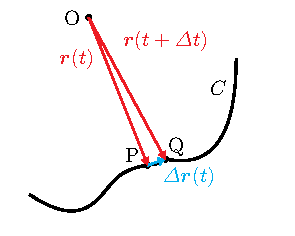
\includegraphics[width=5cm]{picture/vecterana3}
 \caption{接ベクトル}
\label{fig:setuvec}
 \end{center}
\end{figure}

さらにこのベクトルの大きさを1に調整する.それを$\bm{t}$と表すことにすると,
\begin{align}
\bm{t} = \frac { \dot{ \bm{r} } (t) } { \lvert \dot{ \bm{r} } (t) \rvert }
\end{align}
というベクトルが得られる.
$\bm{t}$の大きさは1で,$\dot{\bm{r}}(t)$と同じ方向を向いたベクトルである.
$\bm{t}$を$C$の点Pおける\emph{単位接ベクトル},\index[widx]{せつべくとる@接ベクトル!たんい@単位---}
もしくは\emph{単位接線ベクトル}\index[widx]{せっせんべくとる@接線ベクトル!たんい@単位---|see{単位接ベクトル}}
と呼ぶ.
$\bm{t}$は接線(tangent)の頭文字をとって$\bm{t}$と書いている.
パラメータを表す$t$と被ってしまっているが,ベクトルとスカラーをきちんと使い分ければ
混乱することもないだろう.

$\bm{t}$はパラメータ$t$が微小変化したときの$\bm{r}(t)$の変化の向きを表すベクトルである.
1変数関数におけるグラフの接線と同じように考えれば,
$\bm{t}$は点Pにおいて$C$と接するといえるだろう.

\subsubsection{弧長パラメータ}
さっきまでの話では,パラメータ$t$に対しては何の意味も与えていなかった.
しかし,このパラメータに弧長という意味付けをしてやることにより,
いろいろと便利なことがある.
その話を少ししておこう.

曲線$C$をパラメータ$t$を用いてパラメータ表示して,
$C$上の各点を$\bm{r}(t)$とおく.$C$上に定点$\bm{r}(t_0)$をとり,その点から別の点$\bm{r}(t)$までの
$C$に沿って測った曲線の長さを$s$とおく.
$s$はよく知られているように,
\begin{align}
s = \int _{t_0}^t \lvert \dot{ \bm{r} } (t) \rvert \, \mathrm{d} t
\label{eq:kotyou1} 
\end{align}
と表せる.ちょっとなじみがないという人も
\begin{align}
s = \bigintsss _{t_0}^t \sqrt{ \left( \frac{ \mathrm{d} x }{\mathrm{d} t} \right)^2
+ \left( \frac{ \mathrm{d} y } {\mathrm{d} t} \right)^2 
+ \left( \frac{ \mathrm{d} z } {\mathrm{d} t} \right)^2}  \, \mathrm{d} t
\label{eq:kotyou2} 
\end{align}
と書かれれば納得できるだろう.導出は高校レベルである.
あらためてここでやる必要もあるまい.
この$s$を$C$の点$\bm{r}(t_0)$から点$\bm{r}(t)$までの
\emph{弧長}\index[widx]{こちょう@弧長}と呼ぶ.

$s$と$t$は1対1に対応している.
つまり,$s$の値が決まるとそれに対応するような$t$はただ1つに定まる.
$t$が定まれば$C$上の1点が決まるので,
結局$s$と$C$上の点が1対1に対応していることになる.
すなわち,$s$を$C$を表現するためのパラメータとして採用できるということになる.
曲線$C$を弧長$s$でパラメータ表示したとき,
$s$を\emph{弧長パラメータ}\index[widx]{ぱらめーた@パラメータ!こちょう@弧長---}と呼ぶ.
弧長パラメータを用いるといろいろと便利なことがある.
それを今から見ていこう.

弧長パラメータ$s$を用いたときの$C$の接ベクトルを考えてみよう.
$C$上の各点$\bm{r}(s)$について,
\begin{align*}
\frac{\mathrm{d} \bm{r} (s) }{\mathrm{d} s} = \left[
\begin{array}{c} 
\displaystyle \frac{ \mathrm{d} x }{\mathrm{d}s} \\
\displaystyle \frac{ \mathrm{d} y }{\mathrm{d}s} \\
\displaystyle \frac{ \mathrm{d} z }{\mathrm{d}s} 
\end{array}
\right]
\end{align*}
であるが,これを単に$\bm{r}'(s)$と書き表す.
パラメータが$t$と表された場合には微分を$\dot{ \bm{r} } (t)$と書いたが,
慣例として,弧長パラメータ$s$を用いたときにはこれを$\bm{r}'(s)$と書き表す.
これは慣習的なものだが,慣れてくるとなかなか便利だったりする.

さて,$\bm{r}'(s)$の大きさを考えてみる.式(\ref{eq:kotyou1})と微分積分学の基本定理により
\begin{align*}
 \frac{\mathrm{d} s}{\mathrm{d} s} = \lvert \bm{r}'(s) \rvert 
\end{align*}
である.式(\ref{eq:kotyou1})はパラメータがどんなものであっても成り立つのであったから,
当然弧長パラメータを採用したときでも成り立つべきである.
これにより,
\begin{align*}
\lvert \bm{r}'(s) \rvert = 1
\end{align*} 
を得る.パラメータとして弧長パラメータを採用した場合には,
接ベクトルと単位接ベクトルが一致するのである.
イメージもしやすいし,計算も簡便になるといいことだらけである.
そういうわけで,パラメータとして弧長パラメータを採用することはこれからたくさんあるだろう.

\subsubsection{法線ベクトルと曲率}
さっき求めた曲線の単位接ベクトルの大きさは1である.
いま,パラメータ表示された曲線$C$の点Pにおける単位接ベクトル$\bm{t}$を考えると,
\begin{align*}
\bm{t} \cdot \bm{t} =1
\end{align*}
が成り立つ.この式の両辺をパラメータ$t$で微分してやる.
\begin{align*}
\frac{ \mathrm{d} } {\mathrm{d} t} ( \bm{t} \cdot \bm{t} ) =0
\end{align*}
説明してなかったが,内積についても積の微分公式と同じような公式が成り立っている.
\begin{align}
\frac{ \mathrm{d} } {\mathrm{d} t } (\bm{A} \cdot \bm{B} ) 
= \frac{ \mathrm{d} \bm{A} } { \mathrm{d} t} \cdot \bm{B}
+ \bm{A} \cdot \frac{ \mathrm{d} \bm{B} } { \mathrm{d} t } 
\label{eq:vecsekibibun}
\end{align} 
関数の``積''がベクトルの``内積''に変わっただけで,ほぼ同じ形をしている.
同様の公式が外積やスカラー関数倍に関しても成り立っているのだが,いちいち書く必要もないだろう.
とにかく,式(\ref{eq:vecsekibibun})を用いれば,
\begin{align*}
\frac{ \mathrm{d} \bm{t} } {\mathrm{d} t} \cdot \bm{t} 
+ \bm{t} \cdot \frac{ \mathrm{d} \bm{t} } {\mathrm{d} t} & = 0 \\
\therefore \bm{t} \cdot \frac{ \mathrm{d} \bm{t} } {\mathrm{d} t } & = 0
\end{align*}
となる.内積は順番を変えても結果が変わらないことを用いた.
ベクトルの内積が0ということは,
そのベクトルが直交するということであった.
すなわち,$\bm{t}$の微分$\dot{ \bm{t} }$は$\bm{t}$と直交することになる.
$\bm{t}$は$C$の接線方向のベクトルである.
接線と直交するような直線を\emph{法線}\index[widx]{ほうせん@法線}と呼ぶのであった.
そういうわけで,$\dot { \bm{t} }$を$C$の点Pにおける
\emph{主法線ベクトル}\index[widx]{しゅほうせんべくとる@主法線ベクトル}と呼ぶ.
なぜ法線ベクトルでなく主法線ベクトルと書いているかというと,
いま,3次元空間で考えていて,接線に直交するといってもいろいろな方向があるからだ.
その中でも使いやすい特定の方向のベクトルを抽出して使っているので,
これを主法線ベクトルと呼ぶわけだ.
このベクトルの大きさは1とは限らない.パラメータとして弧長パラメータを用いても無理そうである.
そこで,主法線ベクトルの大きさを1に調整したベクトルを$\bm{n}$と書いて,
\emph{単位主法線ベクトル}\index[widx]{しゅほうせんべくとる@主法線ベクトル!たんい@単位---}と名付けよう.
\begin{align}
\bm{n} = \frac{ \dot{ \bm{t} } } { \lvert \dot { \bm{t} } \rvert}
\label{eq:syuhousen}
\end{align}
ということである.

ここからは,パラメータとして弧長パラメータを採用した場合について考える.
$C$の点Pにおける主法線ベクトル$\bm{t}'$は,$\bm{t}$
の弧長パラメータに対する変化率を表す.
$\bm{t}$の大きさは常に1なので,$\bm{t}'$は実質的には$\bm{t}$
の向きの変化を表していることになるだろう.
これはすなわち,$C$がどのくらい曲がっているかを表す量である.
$\bm{t}'$の大きさ$\lvert \bm{t}' \rvert$を
$C$の点Pにおける\emph{曲率}\index[widx]{きょくりつ@曲率}といい,
$\kappa$で表す.
また,$\kappa$の逆数を$C$の点Pにおける
\emph{曲率半径}\index[widx]{きょくりつ@曲率!はんけい@---半径}といい,
$\rho$と表す.
すなわち,
\begin{align}
\bm{t}' = \kappa \bm{n} = \frac{1}{\rho} \bm{n}
\label{eq:kyokuritu}
\end{align}
である.細かい話は抜きにして結果だけ言えば,点Pにおける$C$の曲率半径$\rho$は
点Pにおいて$C$に接するような円を考えたとき,その円の半径を表すものになっている.
これはパラメータとして弧長パラメータを採用したための結果である.

\subsubsection{従法線ベクトル}
さて,$\bm{t}$と$\bm{n}$の外積を考え,これを$\bm{b}$とおく.
\begin{align}
\bm{b} = \bm{t} \times \bm{n} 
\label{eq:juhousen}
\end{align}
$\bm{b}$は$\bm{t}$にも$\bm{n}$にも直交するベクトルであり,
従って$\bm{b}$も法線方向を向いたベクトルである.
さらに,$\bm{t}$と$\bm{n}$は単位ベクトルで,直交するのであった.
よって$\bm{b}$も単位ベクトルである.
このベクトル
$\bm{b}$を\emph{単位従法線ベクトル}\index[widx]{たんいじゅうほうせん@単位従法線ベクトル}という.

\subsubsection{線素ベクトル}
ここからが本題である.
曲線$C$を弧長パラメータを用いてパラメータ表示して,これを$\bm{r} (s)$とする.
$C$上に点Pを任意にとり,Pにおける$C$の単位接ベクトル$\bm{t}$を考える.
弧長パラメータ$s$を$\mathrm{d} s$だけ変化させたとき,この$\mathrm{d}s$を
点Pにおける$C$の\emph{線素}\index[widx]{せんそ@線素}と呼び,
$\bm{r}(s)$の変化$\mathrm{d} \bm{r}$を$C$の点Pにおける
\emph{線素ベクトル}\index[widx]{せんそ@線素!べくとる@---ベクトル}と呼ぶ.
線素ベクトルは,通常$\mathrm{d} \bm{s}$と書き表すことが多い.
弧長パラメータの変化に向きを付与したようなイメージである.
というのも,
\begin{align*}
\mathrm{d} \bm{r} = \frac{ \mathrm{d} \bm{r} } { \mathrm{d} s} \mathrm{d} s
\end{align*}
であり,弧長パラメータを採用しているときには接ベクトルがそのまま単位接ベクトルとなるのだから
\begin{align*}
\mathrm{d} \bm{r} = \bm{t} \, \mathrm{d} s
\end{align*}
ということになるからだ.
従って,$\mathrm{d} \bm{r}$は$\bm{t}$と同じ向きで,大きさ$\mathrm{d} s$
のベクトルだから,これを
\begin{align}
\mathrm{d} \bm{s} = \bm{t} \, \mathrm{d} s
\label{eq:sensovec}
\end{align}
と表すことにそれほど抵抗はないだろう.

線素と線素ベクトルは,これから場の積分論を展開していくうえで中心的な役割を果たす.

\subsection{曲面の法線ベクトルと面素ベクトル}

これからは空間に存在する曲面$S$について考える.
曲線のときと大体同じ話が続くので,パパっと進むことにしよう.
$S$はパラメータを2種類使ってパラメータ表示できる.
$S$上の各点$\bm{r}$をパラメータ$u, \, v$を用いてパラメータ表示して,
$\bm{r}(u, \, v)$と表すことにする.

\subsubsection{接平面}
パラメータ$u, \, v$はそれぞれ勝手に動くのだが,とりあえず$u$の値を
ある定数$u_0$に固定してみる.そうすると,ベクトル$\bm{r}(u_0, \, v)$
は,あたかも1つのパラメータによってパラメータ表示されるような図形であるとみなすことができる.
パラメータ1つでパラメータ表示されるような図形というのは曲線のことであったから,
この曲線を$S$上の\emph{$v$曲線}と呼ぶことにしよう.
実際には,$u$をどんな値に固定するかによって無限に多くの曲線が得られるわけだが,
それらを全部まとめて$v$曲線と呼ぶのである.
同様にして,$v$を定数$v_0$と固定して$u$を動かしたときに$\bm{r}(u, \, v_0)$
の軌跡として得られる曲線を$S$上の\emph{$u$曲線}と呼ぶ.

曲線があれば接線を考えることができる.
いま,パラメータ表示された曲面$S$上に点Pをとり,その位置ベクトルを$\bm{r}(u, \, v)$とする.
その$u$曲線上の接ベクトルを考えると,これは$\bm{r}(u, \, v)$を
$u$で微分して得られるベクトルであるが,
$v$を定数だと思っているということを考えれば,偏微分を使うべきである.
すなわち,
\begin{align*}
\frac{ \partial \bm{r} } {\partial u} 
\end{align*}
は$S$上の$u$曲線の点Pにおける接ベクトルであるということだ.
略記して,
\begin{align*}
\frac{ \partial \bm{r} } {\partial u} = \bm{r}_u
\end{align*}
と表そう.下付きの添え字で偏導関数を表すというのは以前説明したことである.
同様にして,
\begin{align*}
\frac{ \partial \bm{r} } {\partial v} = \bm{r}_v
\end{align*}
は$S$上の$v$曲線の点Pにおける接ベクトルであることもわかるだろう.

さて,$S$上の点Pにおいて,点Pで接するような2本のベクトル$\bm{r}_u, \, \bm{r}_v$
が得られた.この2本のベクトルは線形独立であると考えていいだろう.
このとき,$\bm{r}_u$と$\bm{r}_v$が貼る平面を
$S$の点Pにおける\emph{接平面}\index[widx]{せつへいめん@接平面}という.

\subsubsection{法線ベクトルと曲面の面積}
さっきの話からも明らかなように,$\bm{r}_u$と$\bm{r}_v$の外積を考えれば,
これは点Pにおける$S$の接平面に垂直なベクトルとなる.
このベクトルを$S$の点Pにおける\emph{法線ベクトル}\index{ほうせんべくとる@法線ベクトル}と呼ぶ.
さらに,法線ベクトルの大きさを1に調整して得られるベクトルを
$S$の点Pにおける\emph{単位法線ベクトル}\index[widx]{ほうせんべくとる@法線ベクトル!たんい@単位---}といい,
これは曲線のときと同じく$\bm{n}$という記号で表す.$\bm{n}$は
\begin{align}
\bm{n} = \frac{ \bm{r}_u \times \bm{r}_v } { \lvert \bm{r}_u \times \bm{r}_v \rvert }
\label{eq:kyokumenhou}
\end{align}
と表されるベクトルである.

\begin{figure}[h]
 \begin{center}
 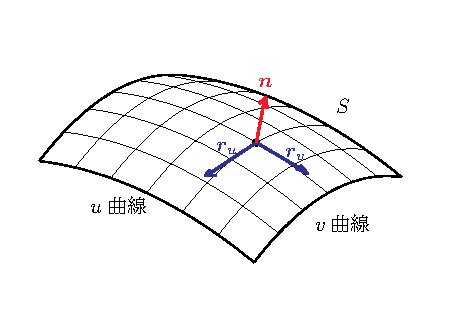
\includegraphics[width=8cm]{picture/vecterana4}
 \caption{曲面の法線ベクトル}
\label{fig:kyokuhousen}
 \end{center}
\end{figure}

ここから曲面$S$の面積を計算することができる.
パラメータ$u, \, v$がそれぞれ$\mathrm{d} u, \, \mathrm{d}v$だけ微小変化したとき,
その変化に対して点Pを表すベクトル$\bm{r}(u, \, v)$が変化し得る領域は,
4点$\bm{r}(u, \, v), \, \bm{r}(u + \mathrm{d}u, \, v), \, 
\bm{r} (u+ \mathrm{d}u, \, v+\mathrm{d}v), \, \bm{r} (u, \, v +\mathrm{d}v )$
を結んだ四角形である.
これらの位置ベクトルは偏微分や全微分の知識を駆使して
\begin{align*}
\bm{r} (u + \mathrm{d} u, \, v) & = \bm{r}(u, \, v) + \bm{r}_u \, \mathrm{d} u \\
\bm{r} ( u + \mathrm{d} u, \, v + \mathrm{d} v) & = 
\bm{r} (u, \, v)+ \bm{r}_u \, \mathrm{d} u + \bm{r}_v \, \mathrm{d} v \\ 
\bm{r} (u, \, v + \mathrm{d} v) & = \bm{r}(u, \, v) + \bm{r}_v \, \mathrm{d}v 
\end{align*}
と求められる.結局のところ,この四角形は
2つのベクトル$\bm{r}_u \, \mathrm{d}u, \, \bm{r}_v \, \mathrm{d}v$が貼る平行四辺形であって,
その面積$\mathrm{d}S$は外積を用いて
\begin{align}
\mathrm{d} S = \lvert \bm{r}_u \times \bm{r}_v \rvert \, \mathrm{d} u \mathrm{d}v
\label{eq:menso}
\end{align}
と表せる.
この$\mathrm{d}S$を点Pにおける$S$の\emph{面素}\index[widx]{めんそ@面素}
もしくは\emph{面積素}\index[widx]{めんせきそ@面積素|see{面素}}と呼ぶ.
$\mathrm{d}S$を$S$全体にわたって足し合わせれば,曲面$S$の面積が求められる.
\begin{align}
S = \iint_S \lvert \bm{r}_u \times \bm{r}_v \rvert \, \mathrm{d} u \mathrm{d} v
\label{eq:kyokumenseki}
\end{align}
これが曲面の面積公式である.
この式はヤコビアンでも表せて,
\begin{align}
S = \bigintsss \! \! \! \! \! \bigintsss_S 
{ \sqrt{ \left( \frac{ \partial ( x, \, y) } {\partial (u, \, v) } \right) ^2
+ \left( \frac{ \partial ( y, \, z) } {\partial (u, \, v) } \right) ^2
+ \left( \frac{ \partial ( z, \, x) } {\partial (u, \, v) } \right) ^2 } \, \mathrm{d}u \mathrm{d}v }
\label{eq:kyokujacobian}
\end{align}
となる.導出は読者に任せることにする.
\begin{itembox}[l]{課題}
半径$r$の球面$S_0$を
\begin{align*}
\renewcommand{\arraystretch}{1}
\bm{r} (\theta, \, \varphi) = \left[
\begin{array}{c}
r \sin \theta \cos \varphi \\
r \sin \theta \sin \varphi \\
r \cos \theta
\end{array}
\right]
\end{align*}
とパラメータ表示する.累次積分を使い,
$\theta$と$\varphi$がそれぞれ独立に
$0 \leq \theta \leq \pi , \, - \pi \leq \varphi \leq \pi$
の範囲を動くときの$S_0$の面積が$4 \pi r^2$になることを確かめよ.

また,3つのベクトル$\dfrac{ \bm{r}_{\theta} }{\lvert \bm{r}_{\theta} \rvert } , \,
\dfrac{ \bm{r}_{\varphi} }{\lvert \bm{r}_{\varphi} \rvert}, \, 
\dfrac{ \bm{r}_{\theta} }{\lvert \bm{r}_{\theta} \rvert} 
\times \dfrac{ \bm{r}_{\varphi} }{\lvert \bm{r}_{\varphi} \rvert} $を求め,$[ \, \cdot \, ]$
を用いた成分表示の形式ではなく
$\bm{e}_x, \, \bm{e}_y , \bm{e}_z$の線形結合の形式で表せ.

以上の計算で得られた3つのベクトルと,$\bm{r}(\theta , \, \varphi)$の
成分中にある$r$を変数とみなし,$\bm{r}(\theta , \, \varphi)$を
$r$で偏微分し,大きさを1に調整することで得られる
$\dfrac{\bm{r}_r}{\lvert \bm{r}_r \rvert}$というベクトル
を眺め,どんなベクトルか,そしてなぜそのような計算結果になったかを考察せよ.
\end{itembox}

\subsubsection{面素ベクトル}
曲面$S$について,$S$上の点Pを任意にとり,その点の位置ベクトルを$\bm{r}(u, \, v)$とおく.
大きさが点Pにおける$S$の面素$\mathrm{d}S$で,
点Pにおける$S$の単位法線ベクトル$\bm{n}$と同じ向きのベクトルを
点Pにおける$S$の\emph{面素ベクトル},\index[widx]{めんそ@面素!べくとる@---ベクトル}
もしくは\emph{面積素ベクトル}\index[widx]{めんせきそ@面積素!べくとる@---ベクトル|see{面素ベクトル}}といい,
$\mathrm{d} \bm{S}$と表す.
\begin{align}
\mathrm{d} \bm{S} = \bm{n} \, \mathrm{d}S 
\label{eq:mensovec}
\end{align}

面素ベクトルは,さも曲面上に面積$\mathrm{d}S$の微小な平面を考え,
その平面の法線ベクトルを表しているようなイメージである.
面素と面素ベクトルも場の積分で活躍する量となる.

\section{場の積分}
これからやるのはベクトル場やスカラー場を積分することである.
積分には積分領域がつきものであるが,
それを一般の曲線や曲面に拡張したい.
1変数関数の積分の場合には積分領域は直線であったし,
重積分のときには積分領域は平面に限られていたのであった.
それに,ベクトル場についてはなにもしていない.
これまでの節で準備はほとんど終わっているので,
これからは実際に積分をやっていこう.

\subsection{スカラー場の線積分}

スカラー場$f(\bm{r})$と空間に存在する曲線$C$を考える.
話を簡単にするため,$C$上の各点$\bm{r}$は,弧長パラメータ$s$を用いて
$\bm{r}(s)$とパラメータ表示されているとしよう.
\subsubsection{今度は最初に厳密な定義}
曲線$C$には端点$\bm{r}(a)$から$\bm{r}(b)$があるとして,
$C$を分割することを考え,その分割を
\begin{align*}
\Delta : \bm{r}(a) = \bm{r}(s_0), \, \bm{r}(s_1), \, \bm{r}(s_2), \, \cdots , \, \bm{r}(s_n) = \bm{r}(b)
\end{align*}
とおく.そして,各分点間での$C$の弧長を
\begin{align*}
\varDelta s_i = \int _{s_{i-1} } ^{s_i} \lvert \bm{r} (s) \rvert \, \mathrm{d}s 
\end{align*}
とおく.さて,2点$\bm{r}(s_{i-1})$から$\bm{r}(s_i)$の間の
$C$上の点から1点$\bm{r}_i$を任意にとり,
その点での$f(\bm{r})$の値$f( \bm{r}_i )$と,分割幅$\varDelta s_i$
をかけて足し合わせる.これでRiemann和の出来上がりである.
\begin{align*}
\sum_{i=1}^n f(\bm{r}_i) \varDelta s_i
\end{align*}
そして,各分割幅の最大値$\delta$が限りなく小さくなるような極限
\begin{align*}
\lim _{\delta \to 0} \sum_{i=1}^n f(\bm{r}_i) \varDelta s_i
\end{align*}
を考え,この極限が分割の仕方や各点$\bm{r}_i$の取り方に依存せずに
一定の値に確定するのであれば,その値をスカラー場$f(\bm{r})$の$C$に沿った
\emph{線積分}\index[widx]{すからーば@スカラー場!のせんせきぶん@---の線積分}といい,
\begin{align*}
\int_C f(\bm{r}) \, \mathrm{d} s 
 \end{align*}
と書き表す.
1変数関数の積分とほとんど変わらない.
\subsubsection{もうちょっと簡単な定義}
さっき書いたのはきちんとした定義であるが,
実用上はもっと簡単に(そして大雑把に)考えた方が何かと便利である.

曲線$C$上に点$\bm{r}(s)$を任意にとり,
その点における線素$\mathrm{d}s$を考え,
この線素と点Pにおける$f(\bm{r})$の値との積$f(\bm{r}(s)) \, \mathrm{d} s $を,
$C$上全体にわたって足し合わせる.
これをスカラー場$f(\bm{r})$の$C$に沿った
\emph{線積分}\index[widx]{すからーば@スカラー場!のせんせきぶん@---の線積分}と呼び,
\begin{align*}
\int_C f( \bm{r} ) \, \mathrm{d}s
\end{align*}
と表す.
やっぱり普通の積分とあまり変わらない気がする.

また,もしも$C$が閉曲線であれば,$\int$記号に丸をくっつけて
$\oint$とし,$C$も閉曲線であることを強調するために$C_0$と添え字をつけて
\begin{align*}
\oint_{C_0} f( \bm{r} ) \, \mathrm{d} s
\end{align*}
と表し,スカラー場$f(\bm{r})$の閉曲線$C_0$に沿った
\emph{周回積分}\index[widx]{すからーば@スカラー場!のしゅうかいせきぶん@---の周回積分}と呼ぶ.
ただし,$\oint$記号を使うかどうかや$C_0$という表し方をするかどうか
は人によって割と差異がある.
この記法に従わない本もかなり多いので注意しよう.

\subsubsection{線積分の計算は簡単である}
線積分の実際の計算は割と簡単である.
``$C$上全体にわたって足し合わせる''というのは結局
弧長パラメータ$s$を考えている範囲全体にわたって動かして,
各点での値を足し合わせるということだから,
もし$s$が$a$から$b$まで動くのであれば,
\begin{align}
\int_C f(\bm{r} ) \, \mathrm{d}s = \int _a^b f(\bm{r} (s) ) \, \mathrm{d} s
\label{eq:sensekikeisan}
\end{align}
という計算をしてやればよいということになる.
$f(\bm{r}(s))$はただの$s$を変数とするスカラーであり,
式(\ref{eq:sensekikeisan})の右辺は$s$に関する普通の積分であるから
簡単に計算できるはずだ.

パラメータ表示は弧長パラメータによるものでなくともよい.
もし弧長パラメータとは限らないパラメータ$t$で$C$がパラメータ表示されていたならば,
まず$C$の線素$\mathrm{d}s$を
\begin{align}
\mathrm{d} s = \lvert \dot {\bm{r} } (t) \rvert  \, \mathrm{d} t
\label{eq:sensopara}
\end{align}
によって求めてから,
\begin{align}
\int_C f(\bm{r} ) \, \mathrm{d} s 
= \int_{t_0}^{t_1} f(\bm{r}(t) )\lvert \dot{ \bm{r} } (t) \rvert \, \mathrm{d} t
\label{eq:sensekibunpara}
\end{align}
という計算をしてやることになる.
$t_0$や$t_1$というのは$C$の端点に対応するパラメータの値であるとした.

線積分を考えるとき,
積分領域となった曲線$C$のことを
\emph{積分経路},\index[widx]{せきぶんけいろ@積分経路}
もしくは単に\emph{経路}\index[widx]{けいろ@経路|see{積分経路}}などと呼ぶ.
また,$C$の端点$\bm{r}(t_0)$と$\bm{r}(t_1)$のことを
それぞれ$C$の\emph{始点}\index[widx]{せきぶんけいろ@積分経路!のしてん@---の始点},
および$C$の\emph{終点}\index[widx]{せきぶんけいろ@積分経路!のしゅうてん@---の終点}という.

\subsubsection{線積分には向きがある}
$C$上全体にわたって足し合わせると書いたが,
そのイメージはパラメータ$t$を$t_0$から$t_1$まで増加させるようなイメージであった.
このパラメータ変化の向きを逆にしたらどうなるだろう? これは,
\begin{align*}
\int_{t_1}^{t_0} f(\bm{r}(t)) \lvert \dot { \bm{r} } (t)  \rvert \, \mathrm{d} t
\end{align*}
という積分を考えることに相当するので,
\begin{align*}
\int_{t_1}^{t_0} f(\bm{r}(t)) \lvert \dot { \bm{r} } (t)  \rvert \, \mathrm{d} t
= - \int_{t_0}^{t_1} f(\bm{r}(t)) \lvert \dot { \bm{r} } (t)  \rvert \, \mathrm{d} t
\end{align*}
ということになる.
どちらも$C$上全体にわたっての和を表しているのに,値が正負逆転していることになってしまう.
これは,``パラメータ変化の向き''によって自然と曲線に向きが付与されたことによるものである.
$C$の端点を始点,終点というように呼んだが,
これは$C$に向きがあるようにイメージしてのことだったのである.

一般に,経路$C$が与えられたとき,
$C$の始点と終点を入れ替えたような経路を$-C$と書き表す.
この書き方は,
\begin{align}
\int_{-C} f( \bm{r} ) \, \mathrm{d} s = - \int_C f( \bm{r} ) \, \mathrm{d}s 
\label{eq:keirogyaku}
\end{align}
という公式が成り立っていることを考えれば受け入れやすいだろう.

さらに,2つの経路$C_1, \, C_2$が与えられ,かつ
$C_1$の終点と$C_2$の始点が一致していたとする.
このとき,$C_1$の始点から出発して終点まで$C_1$に沿って進み,
そしてそこからは$C_2$に沿って$C_2$の終点まで進むような経路を考えることができる.
このような経路を$C_1+C_2$と表す.
この書き方はもちろん,
\begin{align}
\int_{C_1+C_2} f(\bm{r} ) \, \mathrm{d}s = 
\int_{C_1} f(\bm{r}) \, \mathrm{d} s + 
\int_{C_2} f(\bm{r}) \, \mathrm{d} s
\label{eq:keirowa}
\end{align}
という公式が成り立っていることを見越してのことである.
そして,もしも$C_1$の終点と$C_2$の終点が一致していれば,
$C_1+ (-C_2)$という経路も考えることができて,
この経路を$C_1-C_2$と表す.
\begin{align}
\int_{C_1-C_2} f ( \bm{r} ) \, \mathrm{d} s
= \int_{C_1} f(\bm{r}) \, \mathrm{d} s -
\int_{C_2} f(\bm{r}) \, \mathrm{d} s 
\label{eq:keirosa}
\end{align}
という公式が成り立っていることに説明は不要だろう.

\subsubsection{例題を解いてみる}
試しにスカラー場の線積分をいくつか実行してみよう.

経路$C$を$xyz$空間上の点$\mathrm{P} ( -1, \, 0, \, 1)$から
別の点$\mathrm{Q} (1, \, 1, \, 4)$に向かうような線分であるとする.
このとき,スカラー場$f( \bm{r} ) = (x-z)y $の$C$に沿った線積分を求めてみよう.

まず,$\overrightarrow{ \mathrm{PQ} } = 
\left[ 
\renewcommand{\arraystretch}{0.6}
\begin{array}{c}
2 \\
1 \\
3 
\end{array}
\right]$
だから,$C$上の各点$\bm{r}$は
\begin{align*}
\bm{r} (t) = \overrightarrow{ \mathrm{OP} } 
+ t \overrightarrow{ \mathrm{PQ} }
= 
\left[
\renewcommand{\arraystretch}{1}
\begin{array}{c}
-1 + 2t \\
t \\
1+ 3t 
\end{array}
\right]
\qquad (0 \leq t \leq 1) 
\end{align*}
とパラメータ表示できる.
また,
\begin{align*}
\dot{ \bm{r} } (t)  = \left[
\renewcommand{\arraystretch}{1}
\begin{array}{c}
2 \\
1 \\
3
\end{array}
\right]
\end{align*}
であるから,各$t$に対する$C$の線素$\mathrm{d}s$は
\begin{align*}
\mathrm{d} s = \lvert \dot{ \bm{r} } (t)  \rvert \, \mathrm{d}t
= \sqrt{ 2^2 + 1^2 + 3^2 } \, \mathrm{d}t
= \sqrt{14} \, \mathrm{d}t
\end{align*}
ということになる.
さらに,
\begin{align*}
f( \bm{r} (t) ) = ( (-1+2t ) - (1+ 3t ) ) \cdot t 
= -2t - t^2
\end{align*}
であって,従って$f(\bm{r})$の$C$に沿った線積分は
\begin{align*}
\int_C f( \bm{r} ) \, \mathrm{d} s & = 
\int_0^1 (-2t - t^2 ) \cdot \sqrt {14} \, \mathrm{d}t \\
& = \sqrt{14} \left[ -t^2 -\frac{t^3}{3} \right]_0^1 \\
& = - \frac{ 4 \sqrt{14} }{3}
\end{align*}
と求められる.大して難しい計算でもない.

次に,$xyz$空間の経路$C_0$を,
\begin{align*}
\renewcommand{\arraystretch}{1.7}
\bm{r}(t) = \left[
\begin{array}{c}
2 \sin t  \displaystyle \cos \frac{\pi}{6} \\
2 \sin t \displaystyle \sin \frac{\pi}{6} \\
2 \cos t
\end{array}
\right]
= \left[
\renewcommand{\arraystretch}{1}
\begin{array}{c}
\sqrt{3} \sin t \\
\sin t \\
2 \cos t
\end{array}
\right]
\qquad ( 0 \leq t \leq 2 \pi )  
\end{align*}
とパラメータ表示できるような閉曲線であるとして,
この経路$C_0$に沿ってスカラー場$f(\bm{r}) = xyz^2$を線積分してみる.
ただし,$C_0$の向きは$t$が増加するような向きであるとしておく.
\begin{align*}
\dot{ \bm{r} } (t) = \left[
\renewcommand{\arraystretch}{1}
\begin{array}{c} 
\sqrt{3} \cos t \\
\cos t \\
-2 \sin t
\end{array}
\right]
\end{align*}
であるから,各$t$に対する$C_0$の線素$\mathrm{d}s$は
\begin{align*}
\mathrm{d}s & = \lvert \dot{ \bm{r} } (t) \rvert \, \mathrm{d}t 
= \sqrt{ (\sqrt{3} \cos t)^2 + ( \cos t )^2 + ( -2 \sin t )^2 } \, \mathrm{d}t 
= 2 \, \mathrm{d}t
\end{align*}
となる.また,点$\bm{r}(t)$での$f(\bm{r})$の値$f(\bm{r}(t))$は
\begin{align*}
f(\bm{r} (t) ) = 4 \sqrt{3} \sin^2 t \cos ^2 t 
\end{align*}
であり,従って$f(\bm{r})$の$C_0$に沿った線積分は
\begin{align*}
\oint_{C_0} f ( \bm{r} ) \, \mathrm{d} s 
& = \int _0^{2\pi} 4 \sqrt{3} \sin^2 t \cos ^2 t \cdot 2 \, \mathrm{d}t \\
& = \int _0^{2 \pi} 8 \sqrt{3} \cdot \frac{1}{2} \sin ^2 2t \, \mathrm{d} t \\
& = \int _0 ^{2\pi} 4 \sqrt{3} \cdot \frac{ 1- \cos 4t} {2} \, \mathrm{d} t \\
& = \left[ 2 \sqrt{3} \left( t - \frac{1}{4} \sin t \right) \right]_0^{2\pi} \\
& = 4 \sqrt{3} \, \pi
\end{align*}
と求められる.
やっぱり計算は簡単である.

\subsection{スカラー場の面積分}
次は積分領域を曲面に拡張してみよう.
スカラー場$f(\bm{r})$と曲面$S$について考える.
ただし,曲面$S$はパラメータ$u, \, v$でパラメータ表示されているとし,
$S$上の各点は$\bm{r}(u, \, v)$と表せるとしておく.

\subsubsection{厳密だけど簡略な定義}
いちいち積分領域を分割してRiemann和をとっていたら何ページかかるかわかったものではない.
もうめんどくさいのでちょっと簡略化して書いてみる.

$S$上の各点$\bm{r} (u, \, v)$に対し,
その点での$f(\bm{r})$の値$f(\bm{r}(u, \, v))$と
$\bm{r}_u$と$\bm{r}_v$外積の大きさの積
$f(\bm{r} (u, \, v) ) \lvert \bm{r}_u \times \bm{r}_v \rvert$は,
$u, \, v$の2変数関数であるとみなすことができる.
点$\bm{r}(u, \, v)$が$S$上のあらゆる範囲を動くときの
パラメータ$u, \, v$の組$(u, \, v)$が動きうる範囲を$\Omega$とおく.
\footnote{この$\Omega$はギリシャ文字オメガの大文字である.
オームと読むのは電気抵抗を表す特殊な場合だけである.}
この$\Omega$上での$f(\bm{r}(u, \, v)) \lvert \bm{r}_u \times \bm{r}_v \rvert $の2重積分
\begin{align*}
\iint_\Omega f ( \bm{r} (u, \, v) ) \lvert \bm{r}_u \times \bm{r}_v \rvert \, \mathrm{d}u \mathrm{d}v 
\end{align*}
をスカラー場$f(\bm{r} )$の$S$上
での\emph{面積分}\index[widx]{すからーば@スカラー場!のめんせきぶん@---の面積分}といい,
\begin{align*}
\int_S f (\bm{r} ) \, \mathrm{d} S
\end{align*}
と表す.

$S$上の各点における面素$\mathrm{d} S$は
\pageref{eq:menso}ページにあるように,
\begin{align*}
\mathrm{d}S = \lvert \bm{r}_u \times \bm{r}_v \rvert \, \mathrm{d}u \mathrm{d}v
\end{align*}
と書けるのであったから,
面積分というのは,
曲面$S$の各点における面素$\mathrm{d}S$と$f(\bm{r})$の積
$f(\bm{r}) \, \mathrm{d} S$を,
曲面$S$全域にわたって足し合わせるような積分であるといえる.

もし,積分領域$S$が閉じた曲面,つまり閉曲面であれば,
周回積分のときと同じように$S$に添え字をつけて$S_0$と表し,
スカラー場$f(\bm{r})$の閉曲面$S_0$における面積分を
\begin{align*}
\oint_{S_0} f(\bm{r} ) \, \mathrm{d} S
\end{align*}
 と書き表す.
 この点も線積分のときと一緒である.

また,2つの積分領域$S_1$と$S_2$が与えられ,
$S_1$と$S_2$に共通部分がないとする.
このとき,$S_1$と$S_2$を合わせた曲面が考えられる.
そのような曲面を$S_1 + S_2$と表す.線積分と同じように
\begin{align}
\int_{S_1 + S_2 } f(\bm{r} ) \, \mathrm{d}S = 
\int_{S_1} f(\bm{r} ) \, \mathrm{d}S + \int_{S_2} f(\bm{r} ) \, \mathrm{d}S  
\label{eq:mensekibunwa}
\end{align}
という公式が成り立っていることも明らかであろう.
ただし,$S_1$と$S_2$に共通部分があれば式(\ref{eq:mensekibunwa})は成り立たない.
なぜかはちょっと考えればすぐにわかる.

\subsubsection{例題を解いてみよう}
面積分の概念自体は割と簡単に理解できるものであるが,
具体的な計算はちょっと面倒だったりする.

曲面$S$を
\begin{align*} 
S = \Set{ (x, \, y, \, z) | 2x + 3y + 6z = 6 , \, x, \, y, \, z \geq 0 } 
\end{align*}
と定める.このとき,スカラー場$f(\bm{r}) = xyz$の$S$上での面積分を求めてみよう.

ちょっと技巧的だが,曲面$S$の各点$\bm{r}$は
\begin{align*}
\renewcommand{\arraystretch}{1}
\bm{r} (u, \, v) = \left[
\begin{array}{c}
3u \\
2v \\
1 - u - v 
\end{array}
\right]
\end{align*}
とパラメータ表示できる.
具体的には,$x=3u , \, y=2v$と置き換えたのである.
こうすると,分数が消えて後の計算が気持ちよく行える気がする.
$u, \, v$の動きうる範囲は$x, \, y, \, z \geq 0$により
\begin{align*}
3u \geq 0 , \, 
2v \geq 0 , \, 
1 - u - v \geq 0 
\end{align*}
すなわち,
\begin{align*}
0 \leq u \leq 1 , \, 0 \leq v \leq 1-u
\end{align*} 
ということになる.きちんと必要かつ十分な条件になるよう頭をひねってもらいたい.
とにかく,累次積分が使えそうな形になってとりあえず安心である.
\begin{align*}
\Omega = \Set{ (u, \, v) | 0 \leq u \leq 1 , \, 0 \leq v \leq 1-u}
\end{align*}
とおく.この$\Omega$が計算上での積分領域となる.

さて,
\begin{align*}
\bm{r}_u = \left[
\renewcommand{\arraystretch}{1}
\begin{array}{c} 
3 \\
0 \\
-1 
\end{array}
\right]
\, , \, 
\renewcommand{\arraystretch}{1}
\bm{r}_v = \left[
\begin{array}{c}
0 \\
2 \\
-1
\end{array}
\right]
\end{align*}
となり,$\bm{r}_u, \, \bm{r}_v$の外積は
\begin{align*}
\bm{r} _u \times \bm{r}_v = \left[ 
\renewcommand{\arraystretch}{1}
\begin{array}{c}
3 \\
0 \\
-1 
\end{array}
\right]
\times 
\renewcommand{\arraystretch}{1}
\left[
\begin{array}{c}
0 \\
2 \\
-1
\end{array}
\right]
= \left[
\renewcommand{\arraystretch}{1}
\begin{array}{c}
2 \\
3 \\
6
\end{array}
\right]
\end{align*}
となる.ベクトルの外積の成分計算は大丈夫だろうか? もしうろ覚えなら復習しておこう.
ともかく,$\bm{r}_u \times \bm{r}_v$の大きさは
\begin{align*}
\lvert \bm{r}_u \times \bm{r}_v \rvert = \sqrt{ 2^2+3^2+6^2} =7
\end{align*}
となる.よって,点$\bm{r}(u, \, v)$における面素$\mathrm{d}S$は
\begin{align*}
\mathrm{d}S = \lvert \bm{r}_u \times \bm{r}_v \rvert \, \mathrm{d}u \mathrm{d}v
= 7 \, \mathrm{d}u \mathrm{d}v
\end{align*}
と表せることになる.
ここで,
\begin{align*}
f(\bm{r}(u, \, v) ) = 3u \cdot 2v \cdot (1-u-v) = 6uv - 6u^2v - 6uv^2
\end{align*}
であるから,$f(\bm{r})$の$S$上での面積分は
\begin{align*}
\int_S f(\bm{r} ) \, \mathrm{d} S & = 
\iint_\Omega f (\bm{r} (u, \, v) ) \lvert \bm{r}_u \times \bm{r}_v \rvert \, \mathrm{d}u \mathrm{d}v \\
& = 7 \int_0^1 \left( \int_0^{1-u} (6uv-6u^2v-6uv^2) \, \mathrm{d}v \right) \, \mathrm{d}u \\
& = 7 \int_0^1 \Big[ 3uv^2 - 3u^2v^2 - 2uv^3 \Big]_0^{1-u} \, \mathrm{d} u \\
& = 7 \int_0^1 ( 3u(1-u)^2 -3u^2 (1-u)^2 - 2u (1-u)^3 ) \mathrm{d}u \\
& = -7 \int_0^1 u(u-1)^2 ( -3 + 3u + 2(1-u) ) \, \mathrm{d}u \\
& = -7 \int_0^1 u(u-1)^3 \, \mathrm{d}u \\
& = -7 \cdot \frac{ (-1)^3 } {(1+3+1) !} (1-0)^{1+3+1} \\
& = \frac{7}{120}   
\end{align*}
となる.さすがに正攻法でやるとしんどいので,超有名公式
\begin{align}
\int_{\alpha}^{\beta} (x-\alpha)^n (x-\beta)^m \, \mathrm{d}x
= \frac{ (-1)^m }{ (n+m+1)! } (\beta -\alpha )^{n+m+1}
\label{eq:tyouyuumei}
\end{align}
を使わせてもらった.式(\ref{eq:tyouyuumei})を覚えてなくても,
置換積分なり部分積分なりを使えばそれほど苦労せずに計算できる.
暇だったら式(\ref{eq:tyouyuumei})を導いてみるのもいいだろう.

積分までのステップが多い分,計算が長くなったが,
ひとつひとつが何をやっているかをきちんと理解していれば,
このくらいの計算はすらすらとできるはずだ.

次は閉曲面でやってみよう.$xyz$空間の曲面$S_0$を,原点を中心とする半径1の球面と定める.
スカラー場$f(\bm{r})$を$f(\bm{r}) = x+ y^2+ z$と定めたとき,
$f(\bm{r} )$の$S_0$上における面積分を求めてみよう.

まず,$S$をパラメータ表示して
\begin{align*}
\bm{r} (\theta, \, \varphi) = \left[
\renewcommand{\arraystretch}{1}
\begin{array}{c}
\sin \theta \cos \varphi \\
\sin \theta \sin \varphi \\
\cos \theta 
\end{array}
\right]
\quad (0 \leq \theta \leq \pi , \, 0 \leq \varphi \leq 2 \pi)
\end{align*}
として,
\begin{align*}
\Omega = \Set{ (\theta , \, \varphi) | 0 \leq \theta \leq \pi , \, 0 \leq \varphi \leq 2 \pi }
\end{align*}
とおく.
極座標系を直交座標系に焼き直した式と似ている.
まぁ当然なのだが.

$\bm{r}(u, \, v)$をそれぞれのパラメータで偏微分すれば,
\begin{align*}
\bm{r}_\theta = \left[
\renewcommand{\arraystretch}{1}
\begin{array}{c}
\cos \theta \cos \varphi \\
\cos \theta \sin \varphi \\
- \sin \theta
\end{array}
\right] ,  \,
\bm{r}_\varphi = \left[
\renewcommand{\arraystretch}{1}
\begin{array}{c}
 - \sin \theta \sin \varphi \\
\sin \theta \cos \varphi \\
0
\end{array}
\right]
\end{align*}
となる.
$\bm{r}_\theta$と$\bm{r}_\varphi$の外積は
\begin{align*}
\bm{r}_\theta \times \bm{r}_\varphi
=  \left[
\renewcommand{\arraystretch}{1}
\begin{array}{c}
\cos \theta \cos \varphi \\
\cos \theta \sin \varphi \\
- \sin \theta
\end{array}
\right] \times 
\left[
\renewcommand{\arraystretch}{1}
\begin{array}{c}
 - \sin \theta \sin \varphi \\
\sin \theta \cos \varphi \\
0
\end{array}
\right]
= \left[ 
\renewcommand{\arraystretch}{1}
\begin{array}{c}
\sin ^2 \theta \cos \varphi \\
\sin^2 \theta \sin \varphi \\
\sin \theta \cos \theta 
\end{array}
\right]
\end{align*}
となって,その大きさは
\begin{align*}
\lvert \bm{r}_\theta \times \bm{r}_\varphi \rvert
& = \sqrt{ ( \sin ^2 \theta \cos \varphi )^2+
( \sin^2 \theta \sin \varphi )^2 + 
( \sin \theta \cos \theta ) ^2 } \\
& = \sqrt{ \sin^2 \theta ( \sin^2 \theta \cos ^2 \varphi 
+ \sin^2 \theta \sin^2 \varphi + 
\cos^2 \theta ) } \\
& = \sin \theta 
\end{align*}
と求められる.
\begin{align*}
f (\bm{r} (\theta, \, \varphi) ) & = \sin \theta \cos \varphi + (\sin \theta \sin \varphi)^2 + \cos \theta \\
& = \sin \theta \cos \varphi + \sin^2 \theta \sin^2  \varphi + \cos \theta
\end{align*}
だから,そろそろうんざりしてきたところでやっと面積分に入れて,
\begin{align*}
\oint_S f( \bm{r} ) \, \mathrm{d} S 
& = \iint _\Omega (\sin \theta \cos \varphi + \sin^2 \theta \sin^2  \varphi 
+ \cos \theta) \cdot \sin \theta \, \mathrm{d}\theta \mathrm{d} \varphi \\
& = \int_0^{2\pi} \left( \int_0^{\pi} ( \sin^2 \theta \cos \varphi + \sin^3 \theta \sin^2 \varphi
+ \sin \theta \cos \theta  
 ) \, \mathrm{d} \theta \right) \, \mathrm{d} \varphi \\
 & = \int_0^{2 \pi} \Biggl( \int_0^{\pi} 
 \Biggl( \frac{1-\cos 2 \theta }{2} \cos \varphi + \frac{ 3 \sin \theta - \sin 3 \theta }{4} \sin^2 \varphi \\
& \hspace{3cm} + \frac{1}{2} \sin 2 \theta \Biggr) \, \mathrm{d} \theta \Biggr) \, \mathrm{d} \varphi \\
& = \int_0^{2 \pi} \biggl[ \frac{\theta - \frac{1}{2} \sin \theta }{2} \cos \varphi 
+ \frac{ - 3 \cos \theta + \frac{1}{3} \cos 3 \theta }{4} \sin ^2 \varphi \\
& \hspace{3cm} - \frac{1}{4} \cos 2 \theta \biggr]_0^{\pi} \, \mathrm{d} \varphi \\
& = \int_0^{2 \pi} \left( \frac{\pi}{2} \cos \varphi + \frac{4}{3} \sin^2 \varphi \right) \, \mathrm{d} \varphi \\
& = \int _0^{2 \pi} \left( \frac{\pi}{2} \cos \varphi 
+ \frac{4}{3} \frac{ 1 -\cos 2 \varphi }{2} \right) \, \mathrm{d} \varphi \\
& = \left[ \frac{\pi}{2} \sin \varphi + \frac{2}{3} \left( \varphi - \frac{1}{2} \sin 2 \varphi \right)
\right] _0^{2 \pi} \\
& = \frac{4}{3}\pi
\end{align*}
となる.計算量は多いが難易度はそれほど高くはないだろう.

\subsection{ベクトル場の線積分}
スカラー場の次はベクトル場である.さっさと済ませてしまおう.

ベクトル場$\bm{A}(\bm{r})$と空間に存在する曲線$C$を考える.
$C$上の各点$\bm{r}$はパラメータ$t$を用いて$\bm{r}(t)$というように
パラメータ表示されているものとする.
\subsubsection{まずはさくっと定義だけ}
$C$上の各点について,その点における$C$の接ベクトル$\dot{ \bm{r} } (t)$
とその点におけるベクトル場$\bm{A}(\bm{r})$の値$\bm{A}(\bm{r}(t))$
の内積$\bm{A}(\bm{r}(t)) \cdot \dot{ \bm{r} } (t)$を考えると,
これは単なる$t$のスカラーである.
この量の,$C$の始点に相当する$t$の値$t_0$から$C$の端点に相当する$t$の値$t_1$
までの積分をベクトル場$\bm{A}(\bm{r})$の曲線$C$に沿った
\emph{線積分}\index[widx]{べくとるば@ベクトル場!のせんせきぶん@---の線積分}と呼び,
\begin{align*}
\int_C \bm{A}(\bm{r}) \cdot \mathrm{d} \bm{s}
\end{align*}
と表す.

この積分は次のように解釈できる.
$C$上の各点$\bm{r}(t)$に対する$C$の線素ベクトル$\mathrm{d}\bm{s}$は,
その点における$C$の単位接ベクトル$\bm{t}$を用いて
\begin{align*}
\mathrm{d}\bm{s} = \bm{t} \, \mathrm{d} s
\end{align*}
と書き表せるのであった.

ここで,
\begin{align*}
\mathrm{d}s = \lvert \dot{ \bm{r} } (t) \rvert \, \mathrm{d} t
\, , \, \bm{t} = \frac{ \dot{ \bm{r} }(t) } { \lvert \dot{ \bm{r} }(t) \rvert}
\end{align*}
だから,
\begin{align}
\mathrm{d} \bm{s} = \bm{t} \, \mathrm{d} s = \dot{ \bm{r} } (t)  \, \mathrm{d}t
\label{eq:sensoparameta}
\end{align}
となる.

従って,$\bm{A}(\bm{r})$の$C$に沿った線積分というのは,
$C$上の各点$\bm{r}$における線素ベクトル$\mathrm{d}\bm{s}$と
その点にでの$\bm{A}(\bm{r})$との内積をとり,
その値を$C$上全体にわたって足し合わせるような積分であると解釈できる.
\begin{align}
\int_C \bm{A} (\bm{r} ) \cdot \mathrm{d} \bm{s} 
= \int_{t_0}^{t_1} \bm{A} ( \bm{r} (t) ) \cdot \dot{ \bm{r} }(t) \, \mathrm{d} t
\label{eq:sensekibunvec}
\end{align}  
と表したのはむしろ当然であるといえるだろう.

ベクトル場の線積分はさっき書いた形式とは似ても似つかぬ形式で書かれることがある.
というのも,$C$上の線素ベクトル$\mathrm{d}\bm{s}$は
\begin{align*}
\mathrm{d} \bm{s} = \dot{ \bm{r} }(t) \, \mathrm{d} t = \left[
\begin{array}{c}
\displaystyle \frac{ \mathrm{d} x }{\mathrm{d} t } \mathrm{d} t \\
\displaystyle \frac{ \mathrm{d} y }{\mathrm{d} t } \mathrm{d} t \\
\displaystyle \frac{ \mathrm{d} z }{\mathrm{d} t } \mathrm{d} t 
\end{array}
\right]
\end{align*}
と表せるが,これは,
\begin{align*}
\left[
\begin{array}{c}
\displaystyle \frac{ \mathrm{d} x }{\mathrm{d} t } \mathrm{d} t \\
\displaystyle \frac{ \mathrm{d} y }{\mathrm{d} t } \mathrm{d} t \\
\displaystyle \frac{ \mathrm{d} z }{\mathrm{d} t } \mathrm{d} t 
\end{array}
\right] = \left[
\renewcommand{\arraystretch}{1}
\begin{array}{c}
\mathrm{d} x \\
\mathrm{d} y \\
\mathrm{d} z
\end{array}
\right]
\end{align*}
となることから,
\begin{align*}
\mathrm{d} \bm{s} = \left[
\renewcommand{\arraystretch}{1}
\begin{array}{c}
\mathrm{d} x \\
\mathrm{d} y \\
\mathrm{d} z 
\end{array}
\right]
\end{align*}
と表せることになる.従って,
ベクトル場$\bm{A}(\bm{r})$が
\begin{align*}
\bm{A} (\bm{r} ) = \left[
\renewcommand{\arraystretch}{1}
\begin{array}{c}
f( \bm{r} ) \\
g( \bm{r} ) \\
h ( \bm{r} ) \\
\end{array}
\right]
\end{align*}
と成分表示されていたとすると,$\bm{A}(\bm{r})$の$C$に沿った線積分は
\begin{align}
\int_C \bm{A} ( \bm{r} ) \cdot \mathrm{d} \bm{s} =
\int_C ( f( \bm{r} ) \, \mathrm{d} x + g( \bm{r} ) \, \mathrm{d} y + h(\bm{r}) \, \mathrm{d}z )
\label{eq:sensekibunvecseibun} 
\end{align}
ということになる.
式(\ref{eq:sensekibunvecseibun})の右辺だけを見せられて,これが
ベクトル場の線積分を表しているとわかる人はまずいないであろう.
あるいはちょっと書き方を変えて
\begin{align*}
\int_C ( f \, \mathrm{d} x + g \, \mathrm{d} y + h \, \mathrm{d}z )
\end{align*}
なんて書かれたらどうだろうか? カッコを書かずに
\begin{align*}
\int_C f \, \mathrm{d} x + g \, \mathrm{d} y + h \, \mathrm{d}z
\end{align*}
なんて書くような人もいる.
こういう記法はベクトル場という概念をあまり重視しない場面でよく出てくる.
とはいえ,本書は電磁気学を学ぶことを視野に入れているため,
こういった表現は使わないことにする.

スカラー場の線積分と同じように,もし積分領域が閉曲線であれば,
その曲線は$C_0$と表され,$\bm{A}(\bm{r})$の$C_0$に沿った線積分も
\begin{align*}
\oint_{C_0} \bm{A} ( \bm{r} ) \cdot \mathrm{d} \bm{s} 
\end{align*}
と書き表される.
そして,この積分はベクトル場$\bm{A}(\bm{r})$の閉曲線$C_0$に沿った
\emph{周回積分}\index[widx]{べくとるば@ベクトル場!のしゅうかいせきぶん@---の周回積分}
と呼ばれることも同じである.

\subsubsection{例題を解いてみる}
ベクトル場の線積分を実際に計算してみよう.
いま,曲線$C$を点$\mathrm{P} ( 1,\, 0, \ 1)$から別の点$\mathrm{Q}(0, \, 1, \, 1 )$
に向かう線分とする.
ベクトル場$\bm{A} (\bm{r})$を
\begin{align*}
\bm{A} (\bm{r}) = \left[
\renewcommand{\arraystretch}{1}
\begin{array}{c}
y \\
x \\
\displaystyle \sin^2 \frac{\pi}{2} z
\end{array}
\right]
\end{align*}
と定めたときの$\bm{A}(\bm{r})$の$C$に沿った線積分を求めてみよう.

$C$上の各点$\bm{r}$は
\begin{align*}
\overrightarrow{\mathrm{PQ}} = \left[
\renewcommand{\arraystretch}{1}
\begin{array}{c}
-1 \\
1 \\
0
\end{array}
\right]
\end{align*}
であることから,
\begin{align*}
\bm{r}(t) = \overrightarrow{\mathrm{OP}} + t \overrightarrow{\mathrm{PQ}} 
= \left[
\renewcommand{\arraystretch}{1}
\begin{array}{c} 
1 - t \\
t \\
1 
\end{array}
\right]
\qquad (0 \leq t \leq 1)
\end{align*}
とパラメータ表示できる.
これはつまり,
\begin{align*}
\begin{aligned}
x & = 1 - t \\
y & = t \\
z & = 1
\end{aligned}
\qquad (0 \leq t \leq 1)
\end{align*}
ということなので,これを$\bm{A}(\bm{r})$に代入して
\begin{align*}
\bm{A} ( \bm{r}(t) ) = \left[
\renewcommand{\arraystretch}{1}
\begin{array}{c} 
t \\
1- t \\
\displaystyle \sin^2 \frac{\pi}{2}
\end{array}
\right]
= \left[
\renewcommand{\arraystretch}{1}
\begin{array}{c}
t \\
1- t \\
1
\end{array}
\right]
\end{align*}
となる.

また,
\begin{align*}
\dot{ \bm{r} } (t) = \left[
\renewcommand{\arraystretch}{1}
\begin{array}{c}
-1 \\
1 \\
0
\end{array}
\right]
\end{align*}
であり,
\begin{align*}
\mathrm{d}\bm{s} = \dot{ \bm{r}}(t) \, \mathrm{d}t =\left[
\renewcommand{\arraystretch}{1}
\begin{array}{c}
- \mathrm{d} t \\
\mathrm{d} t \\
0
\end{array}
\right]
\end{align*}
だから,
\begin{align*}
\bm{A} (\bm{r}(t)) \cdot \mathrm{d}\bm{s}
= \left[
\renewcommand{\arraystretch}{1}
\begin{array}{c} 
t \\
1-t \\
1
\end{array}
\right] \cdot \left[
\renewcommand{\arraystretch}{1}
\begin{array}{c}
- \mathrm{d}t \\
\mathrm{d} t \\
0
\end{array}
\right]
= ( 1 -2t ) \, \mathrm{d} t 
\end{align*}
となる.

従って,$\bm{A}(\bm{r})$の$C$に沿った線積分は
\begin{align*}
\int_C \bm{A}(\bm{r}) \cdot \mathrm{d} \bm{s} & =
\int_0^1 (1 - 2t ) \, \mathrm{d} t \\
& = \biggl[ t - t^2  \biggr]_0^1 \\
& =0
\end{align*}
ということになる.なんだか拍子抜けするような結果だが,
積分した結果が0になるなんていうようなことはよくあることである.

もう1問くらい解いてみようか.
いま,閉曲線$C_0$を点$(1, \, 0, \, 0)$を始点とし,$xy$平面上にある
原点中心,半径1の円の周上を$z$軸正方向から見て反時計回りに1周するような経路だとして,
ベクトル場$\bm{A}(\bm{r})$を
\begin{align*}
\bm{A} ( \bm{r} ) = \left[
\renewcommand{\arraystretch}{1}
\begin{array}{c}
3x - y + 2z \\
x + y -2z^2 \\
2xz - y^2 - z^3
\end{array}
\right]
\end{align*}
と定めたときの$\bm{A}(\bm{r})$の$C_0$上での周回積分を求めてみる.

まず,$C_0$上の各点$\bm{r}$は
\begin{align*}
\bm{r} (t) = \left[
\renewcommand{\arraystretch}{1}
\begin{array}{c}
\cos t \\
\sin t \\
0
\end{array}
\right]
\qquad (0 \leq t \leq 2 \pi)
\end{align*}
とパラメータ表示できる.
これはすなわち
\begin{align*}
\begin{aligned}
x & = \cos t \\
y & = \sin t \\
z & = 0
\end{aligned}
\qquad (0 \leq t \leq 2 \pi)
\end{align*}
ということだから,$\bm{A}(\bm{r}(t))$は
\begin{align*}
\bm{A}(\bm{r}(t)) = \left[
\renewcommand{\arraystretch}{1}
\begin{array}{c}
3 \cos t - \sin t + 2 \cdot 0 \\
\cos t + \sin t - 2 \cdot 0^2 \\
2 \cos t \cdot 0 - \sin^2 t - 0^3 
\end{array}
\right] = \left[
\renewcommand{\arraystretch}{1}
\begin{array}{c}
3 \cos t - \sin t \\
\cos t + \sin t \\
- \sin ^2 t 
\end{array}
\right]
\end{align*}
となる.

さて,
\begin{align*}
\dot{ \bm{r} } (t) = \left[
\renewcommand{\arraystretch}{1}
\begin{array}{c} 
- \sin t \\
\cos t \\
0
\end{array}
\right]
\end{align*}
だから,
\begin{align*}
\bm{A}(\bm{r}(t)) \cdot \dot{ \bm{r} }(t) & = \left[
\renewcommand{\arraystretch}{1}
\begin{array}{c}
3 \cos t - \sin t \\
\cos t + \sin t \\
- \sin^2 t 
\end{array}
\right] \cdot \left[
\renewcommand{\arraystretch}{1}
\begin{array}{c}
- \sin t \\
\cos t \\
0
\end{array}
\right] \\
& = (3 \cos t -\sin t ) (- \sin t) + ( \cos t + \sin t ) \cos t \\
& = 1 - 2 \cos t 
\end{align*}
となる.

従って,$\bm{A}(\bm{r})$の$C_0$に沿った周回積分は
\begin{align*}
\oint_{C_0} \bm{A} (\bm{r} ) \cdot \mathrm{d} \bm{s} & 
= \int_0^{2 \pi} (1- 2 \cos t) \, \mathrm{d} t \\
& = \biggl[ t - 2 \sin t \biggr]_0^{2 \pi} \\
& = 2 \pi  
\end{align*}
と求められる.大して難しい計算というわけでもない.
\subsubsection{ベクトル場の線積分の解釈}
ベクトル場の線積分が何を表しているか考えてみよう.
$\bm{A} ( \bm{r} ) \cdot \mathrm{d} \bm{s}$という量は,
$\bm{A}(\bm{r} )$と$\mathrm{d} \bm{s}$の内積であって,
その値は$\bm{A}(\bm{r} )$と$\mathrm{d} \bm{s}$の向きがそろっていれば大きくなり,
その向きが垂直に近づくと小さくなる.
もちろん,$\bm{A}(\bm{r} )$と$\mathrm{d} \bm{s}$の大きさが大きくなれば
その内積も大きくなる.
その傾向は積分しても変わらない.
すなわち,ベクトル場の線積分というのは,
ベクトル場がその曲線に沿って
どの程度の強さの分布をしているかを表すのである.
これは,力学における仕事に例えてみるとわかりやすい.
いま,物体を曲線$C$に沿って動かしたとする.
位置$\bm{r}$において物体に加えた力が$\bm{F}(\bm{r})$であれば,
$\bm{F}(\bm{r})$のした仕事$W$は
\begin{align}
W = \int_C \bm{F}(\bm{r}) \cdot \mathrm{d} \bm{s}
\label{eq:work}
\end{align}
と定義されるのであった.この$W$は$\bm{F}(\bm{r})$の大きさが大きければその値は大きくなるが,
それだけではいけない.$\bm{F}(\bm{r})$の向きが$C$に沿っていなければ
$W$は大きくはならない.
これならばイメージしやすいだろう.
これは,さっき言っていたこととほとんど同じことである.

では,周回積分ならばどうだろう? ベクトル場の周回積分というのは
ベクトル場の閉曲線に沿った線積分のことであった.
線積分がベクトル場の積分経路に沿った分布がどれだけあるかを表しているというのであれば,
閉曲線に沿った線積分,すなわち
周回積分というのはそのベクトル場が
どれだけ強い渦を巻いているかを表しているかを表すと解釈するのが自然であろう.
あるベクトル場を閉曲線に沿って周回積分して,
もしその値が大きければ,
そのベクトル場は閉曲線に沿ってぐるぐる渦を巻くような分布をしているということになるからだ.

\subsubsection{渦なし場とスカラーポテンシャル}
さて,ベクトル場の周回積分というのはベクトル場がどのくらい強い渦を巻いているかを表すのであった.
今回は,その値が0であるようなベクトル場を考えてみる.
すなわち,閉曲線$C_0$について
\begin{align}
\oint_{C_0} \bm{A}(\bm{r}) \cdot \mathrm{d} \bm{s} = 0
\label{eq:uzunasi}
\end{align}
をみたすようなベクトル場$\bm{A}(\bm{r})$について考えてみる.
もし式(\ref{eq:uzunasi})が\.任\.意\.の閉曲線$C_0$について成り立つならば,
$\bm{A}(\bm{r})$は\emph{渦なし場}\index[widx]{うずなしば@渦なし場}であるという.
\footnote{``渦なし場''という用語は書籍によって表記にかなりのブレがある.
とはいえ,意味は通じるようになっているはずだから混乱することはないだろう.}
ある\.特\.定\.の閉曲線$C_0$について式(\ref{eq:uzunasi})が成り立つのでは不十分である.
あくまでどんな閉曲線であっても式(\ref{eq:uzunasi})が成り立たなければ渦なし場とはいわない.
もし式(\ref{eq:uzunasi})が成り立たないような閉曲線が1つでもあれば,
そのベクトル場はその閉曲線に沿って渦を巻いているとみなすのである.
\footnote{これからの議論を円滑に進めるうえでは
積分領域が単に閉曲線であるだけでは不十分なのであるが,
そのような面倒なことは考えないことにする.}

さて,式(\ref{eq:uzunasi})が任意の閉曲線で成り立つような渦なし場$\bm{A}(\bm{r})$について,
$\bm{A}(\bm{r})$を2つの曲線$C_1, \, C_2$に沿って線積分することを考える.
ただし,$C_1$の始点と$C_2$の始点,および$C_1$の終点と$C_2$の終点は一致するものとする.
スタートとゴールが一致する2つの経路$C_1, \, C_2$について考えるといえばわかりやすいだろうか.
このとき,$C_1$の始点からスタートして$C_1$に沿って$C_1$の終点に進み,
そこからは$C_2$に沿って$C_2$の終点から$C_2$の始点まで進むような経路を考えれば,
このような曲線は閉曲線である.これは各自図を描いて確認してほしい.
\pageref{eq:keirosa}ページには,このような経路は$C_1-C_2$と表し,
さらに,
\begin{align*}
\oint_{C_1-C_2} \bm{A}(\bm{r}) \cdot \mathrm{d}\bm{s}
= \int_{C_1} \bm{A}(\bm{r}) \cdot \mathrm{d} \bm{s} -
\int_{C_2} \bm{A}(\bm{r}) \cdot \mathrm{d} \bm{s}
\end{align*}
が成り立つのだと書いてある.
今回は$C_1-C_2$が閉曲線なので左辺の積分が周回積分となっている.
さて,$\bm{A}(\bm{r})$は渦なし場であったから,
\begin{align*}
\oint_{C_1-C_2} \bm{A}(\bm{r}) \cdot \mathrm{d}\bm{s} = 0
\end{align*}
が成り立つので,
\begin{align}
\int_{C_1} \bm{A}(\bm{r}) \cdot \mathrm{d} \bm{s}
=  \int_{C_2} \bm{A}(\bm{r}) \cdot \mathrm{d} \bm{s}
\label{eq:uzunasisekibun}
\end{align}
が成り立つことがわかる.
$C_1$と$C_2$それぞれの始点,終点が一致するよう任意にとった閉曲線である.
つまり,式(\ref{eq:uzunasisekibun})が示すのは,
渦なし場の線積分は始点と終点によってのみその値が決まり,
途中の経路には依存しないということである.

というわけで,渦なし場$\bm{A}(\bm{r})$について,次のような式で定義されるスカラー$\phi(\bm{r})$を考える.
\begin{align}
\phi (\bm{r}) - \phi (\bm{r}_0 )= - \int_{\bm{r}_0}^{\bm{r}} \bm{A}(\bm{r}) \cdot \mathrm{d} \bm{s}
\label{eq:sukara}
\end{align}
$\bm{r}_0$というのはどこかに適当にとった基準点である.別にどこでもいい.$\bm{r}_0$がどこだろうと大した問題ではない.
積分範囲を$\bm{r}_0$から$\bm{r}$としてあるが,これは$\bm{r}_0$を始点,$\bm{r}$を終点とする適当な曲線をとり,
その曲線に沿って$\bm{A}(\bm{r})$を線積分してくれという意味である.
どの曲線をとるかで$\phi(\bm{r})$の値が変わらないことはさっき確認したとおりである.
$\phi(\bm{r})$は$\bm{r}$によって値がきまる1つのスカラーである.
$\phi(\bm{r})$を$\bm{A}(\bm{r})$の
\emph{スカラーポテンシャル}\index[widx]{すからー@スカラー!ぽてんしゃる@ポテンシャル}という.
式にマイナスが付いているのが気になるが,そこは気にせずにいよう.
別にマイナスがついていようがいまいが本質は変わらない.
しかし,物理学においてはスカラーポテンシャルにエネルギーという物理的意味
を見出したいがためにマイナスをつけている.
数学の専門書の中ではマイナスがついていない定義が採用されていることも多い.

スカラーポテンシャルに関して深堀りするのはやめておこう.
とにかく,渦なしの場に対しては経路によらない線積分としてスカラーポテンシャルが定義できるのである.
渦のある場に対してはこのようなことは言えない.線積分に値が経路によって変化してしまうためである.

\subsubsection{スカラーポテンシャルの例}
あらゆる閉曲線について,その閉曲線に沿ったベクトル場の周回積分が0になるような
ベクトル場など本当に存在するのか怪しいところである.
ここでは,典型的な渦なし場について考えてみる.
知っている人にとっては茶番のようであるが,しばらくは付き合ってほしい.

さて,ベクトル場$\bm{E}(\bm{r})$を
\begin{align}
\bm{E}(\bm{r}) = \frac{1}{4 \pi \varepsilon_0} \frac{q}{r^3} \bm{r}
\label{eq:seidenba}
\end{align}
と定める.式中の$r$はベクトル$\bm{r}$の大きさ$\lvert \bm{r} \rvert$を略記したものだと考えてほしい.
曲線$C$を任意にとり,その始点を$\bm{r}_A$,終点を$\bm{r}_B$とおく.
$\bm{E}(\bm{r})$を$C$に沿って積分したいのだが,ここは極座標系で考えるのが吉である.

極座標系$(r, \, \theta , \, \varphi)$とDescartes座標系の関係は
\begin{align*}
x & = r \sin \theta \cos \varphi \\
y & = r \sin \theta \sin \varphi \\
z & = r \cos \theta
\end{align*}
であった.ところで,$x, \, y, \, z$の全微分は
\begin{align*}
\mathrm{d}x & = \frac{\partial x} {\partial r} \mathrm{d} r 
+ \frac{\partial x} {\partial \theta} \mathrm{d} \theta 
+ \frac{\partial x} {\partial \varphi} \mathrm{d} \varphi \\
\mathrm{d}y & = \frac{\partial y} {\partial r} \mathrm{d} r 
+ \frac{\partial y} {\partial \theta} \mathrm{d} \theta 
+ \frac{\partial y} {\partial \varphi} \mathrm{d} \varphi \\
\mathrm{d}z & = \frac{\partial z} {\partial r} \mathrm{d} r 
+ \frac{\partial z} {\partial \theta} \mathrm{d} \theta 
+ \frac{\partial z} {\partial \varphi} \mathrm{d} \varphi 
\end{align*}
であったから,式中にある偏微分を実際に行ってみると,
\begin{align}
\begin{aligned}
\mathrm{d} x & = \sin \theta \cos \varphi \, \mathrm{d} r 
 + r \cos \theta \cos \varphi \, \mathrm{d} \theta 
 - r \sin \theta \sin \varphi \, \mathrm{d} \varphi \\
\mathrm{d} y & = \sin\theta \sin \varphi \, \mathrm{d}r
 + r \cos \theta \sin \varphi \, \mathrm{d}\theta 
 + r \sin \theta \cos \varphi \, \mathrm{d} \varphi \\
\mathrm{d} z & = \cos \theta \, \mathrm{d} r  - r \sin \theta \, \mathrm{d} \theta
\label{eq:Deckyokubibun}
\end{aligned}
\end{align}
となる.後はDescartes座標系における基底$\bm{e}_x, \, \bm{e}_y, \, \bm{e}_z$
を極座標系における基底$\bm{e}_r, \, \bm{e}_\theta, \, \bm{e}_\varphi$に焼き直すだけだが,
それは\pageref{eq:kyokuDeckitei}ページに書いてあって,もう一度式を書くと
\begin{align*}
\bm{e}_r & = & \sin \theta \cos \varphi \, \bm{e}_x & & + \sin \theta \sin \varphi \, \bm{e}_y &
& + \cos \theta \, \bm{e}_z & \\
\bm{e}_\theta & = & \cos \theta \cos \varphi \, \bm{e}_x & & + \cos \theta \sin \varphi \, \bm{e}_y & 
& -  \sin \theta \,  \bm{e}_z & \\
\bm{e}_\varphi & = & - \sin \varphi \, \bm{e}_x & & + \cos \varphi \, \bm{e}_y &
\end{align*}
であった.行列を用いて書けば,
\begin{align*}
\renewcommand{\arraystretch}{1}
\left[
\begin{array}{ccc}
\bm{e}_r & \bm{e}_\theta & \bm{e}_\varphi
\end{array}
\right]
= \left[
\renewcommand{\arraystretch}{1}
\begin{array}{ccc}
\bm{e}_x & \bm{e}_y & \bm{e}_z 
\end{array}
\right]
\left[
\renewcommand{\arraystretch}{1}
\begin{array}{ccc} 
\sin \theta \cos \varphi & \cos \theta \cos \varphi & - \sin \varphi \\
\sin \theta \sin \varphi & \cos \theta \sin \varphi & \cos \varphi \\
\cos \theta & - \sin \theta & 0
\end{array}
\right]
\end{align*}
となる.ここから連立方程式を解く要領で係数行列の逆行列を求めていけばいいのだが,
さすがに面倒なので結果だけ書かせてもらう.
\begin{align}
\begin{aligned}
\bm{e}_x & = & \sin \theta \cos \varphi \, \bm{e} _r & & 
+ \cos \theta \cos \varphi \, \bm{e}_\theta & & - \sin \varphi \, \bm{e}_\varphi & \\
\bm{e}_y & = & \sin \theta \sin \varphi \, \bm{e}_r & & 
+ \cos \theta \sin \varphi \, \bm{e}_\theta & & 
+ \cos \varphi \, \bm{e}_\varphi & \\
\bm{e}_z & = & \cos \theta \, \bm{e}_r & & - \sin \theta \, \bm{e}_\theta &
\label{eq:Deckyokukitei}
\end{aligned}
\end{align}
実は,ちょっと線形代数学の知識に明るかったりするとこの計算は暗算でもできたりする.
まぁそのテクニックに関しては線形代数学を学べば嫌でも身につくだろう.

さて,$C$の線素ベクトル$\mathrm{d}\bm{s}$は\pageref{eq:sensekibunvecseibun}
ページあたりに 
\begin{align}
\mathrm{d} \bm{s} = \mathrm{d} x \, \bm{e}_x + \mathrm{d} y \, \bm{e}_y + \mathrm{d} z \, \bm{e}_z
\label{eq:sensoDec}
\end{align}
と表せると書いてあるので,これに式(\ref{eq:Deckyokubibun})と式(\ref{eq:Deckyokukitei})
を代入して頑張って計算すると
\begin{align}
\mathrm{d} \bm{s} = \mathrm{d} r \, \bm{e}_r 
+ r \, \mathrm{d}\theta \, \bm{e}_\theta
+ r \sin \theta \, \mathrm{d} \varphi \, \bm{e}_\varphi
\label{eq:sensokyoku}
\end{align}
となる.計算が面倒なだけなのでここには途中計算は載せない.

また,$\bm{r} = r \, \bm{e}_r$なので
\begin{align*}
\bm{E}(\bm{r}) \cdot \mathrm{d} \bm{s} 
& = \frac{1}{4 \pi \varepsilon_0} \frac{q}{r^3} r \, \bm{e}_r \cdot 
(\mathrm{d} r \, \bm{e}_r 
+ r \, \mathrm{d}\theta \, \bm{e}_\theta
+ r \sin \theta \, \mathrm{d} \varphi \, \bm{e}_\varphi) \\
& = \frac{1}{4 \pi \varepsilon_0} \frac{q}{r^2} \mathrm{d}r
\end{align*}
と計算できる.
計算には$\bm{e}_r, \, \bm{e}_\theta, \, \bm{e}_\varphi$が互いに直交する単位ベクトルであることを用いた.
内積に$\mathrm{d}\theta$と$\mathrm{d}\varphi$は残らず,$\mathrm{d}r$のみが残った.
これが意味するのは,$C$上全体にわたって積分をしていくときに$r, \, \theta, \, \varphi$はすべて変化するが,
そのなかでも$\theta$と$\varphi$の変化は積分値に影響を与えないということだ.

従って,$\bm{E}(\bm{r})$の$C$に沿った線積分は
\begin{align*}
\int_{C} \bm{E}(\bm{r}) \cdot \mathrm{d} \bm{s}
& = \int_{r_A}^{r_B}  \frac{1}{4 \pi \varepsilon_0} \frac{q}{r^2}  \mathrm{d}r \\
& = \left[ - \frac{1}{4 \pi \varepsilon_0} \frac{q}{r} \right]_{r_A}^{r_B} \\
& = - \left( \frac{1}{4 \pi \varepsilon_0} \frac{q}{r_B} 
- \frac{1}{4 \pi \varepsilon_0} \frac{q}{r_A} \right)
\end{align*}
となり,積分値が$C$の始点と終点だけで決まることがわかる.そこで,
\begin{align}
\phi (\bm{r} ) = \frac{1}{4 \pi \varepsilon_0} \frac{q}{r}
\label{eq:seidenpotential}
\end{align}
とおけば,
\begin{align}
\phi(\bm{r}) - \phi ( \bm{r}_0) = - \int_{\bm{r}_0}^{\bm{r}} \bm{E}(\bm{r}) \cdot \mathrm{d}\bm{s}
\label{eq:seidensekibun} 
\end{align}
が積分経路$C$によらずに成り立つことになる.
この$\phi(\bm{r})$が何を表しているかとかそういうことは話さなくていいだろう.
もし始点と終点が一致するような任意の積分経路,すなわち閉曲線$C_0$に沿って$\bm{E}(\bm{r})$
を積分すれば,その始点,および終点を$\bm{r}_0$として式(\ref{eq:seidensekibun})により,
\begin{align*}
\oint_{C_0} \bm{E}(\bm{r}) \cdot \mathrm{d} \bm{s} 
= - ( \phi (\bm{r}_0) - \phi ( \bm{r}_0) ) = 0
\end{align*}
つまり,任意の閉曲線$C_0$について
\begin{align}
\oint_{C_0} \bm{E}(\bm{r}) \cdot \mathrm{d} \bm{s} = 0
\label{eq:seidenbauzunasi}
\end{align}
が成り立ち,式(\ref{eq:seidenba})で定義されるベクトル場$\bm{E}(\bm{r})$
は渦なし場であることがわかる.

計算は非常に面倒であったが,これまでの事項のよい復習になったはずだ.

\subsection{ベクトル場の面積分}
ベクトル場の線積分の次はベクトル場の面積分である.
ちゃちゃっと済ませてしまおう.

ベクトル場$\bm{A}(\bm{r})$と曲面$S$を考える.
$S$はパラメータ表示されており,これを$\bm{r}(u, \, v)$としよう.
ただし注意点として,$S$には裏と表があり,それらは区別できるものとする.
\subsubsection{すべては定義からスタートする}
$S$上の各点$\bm{r}(u, \, v)$について,$\bm{r}_u \times \bm{r}_v$というベクトル
とその点における$\bm{A}(\bm{r})$の値$\bm{A}(\bm{r}(u, \, v))$の内積
$\bm{A}(\bm{r}(u, \, v)) \cdot (\bm{r}_u \times \bm{r}_v ) $は,$u, \, v$によって決まるスカラーである.
$\bm{r}(u, \, v)$が$S$上の各点を動くときのパラメータの組$(u, \, v)$の動く範囲を$\Omega$として,
2重積分
\begin{align*}
\iint_{\Omega} \bm{A}( \bm{r} (u, \, v) ) \cdot 
( \bm{r}_u \times \bm{r}_v ) \, \mathrm{d}u\mathrm{d}v
\end{align*}
をベクトル場$\bm{A}(\bm{r})$の曲面$S$上での
\emph{面積分}\index[widx]{べくとるば@ベクトル場!のめんせきぶん@---の面積分}と呼び,
\begin{align*}
\int_S \bm{A}(\bm{r}) \cdot \mathrm{d} \bm{S} 
\end{align*}
と表す.あるいは,$S$上の各点における単位法線ベクトル$\bm{n}$
とその点における$S$の面素$\mathrm{d}S$を用いて
\begin{align*}
\int_S \bm{A}(\bm{r}) \cdot \bm{n} \, \mathrm{d} S 
\end{align*}
と表してもいい.どちらも同じ積分を表す.
スカラー場の面積分とほとんど同じ定義である.

もし積分領域$S$が閉曲面であれば,これを$S_0$と表して,
$\bm{A}(\bm{r})$の$S_0$上での面積分は
\begin{align*}
\oint_{S_0} \bm{A}(\bm{r}) \cdot \mathrm{d}\bm{S}
\end{align*}
と表すのがお約束である.
この点もスカラー場の面積分のときと同じである.

この積分も線積分のときと同じように解釈できて,
$S$の点$\bm{r}(u, \, v)$における面素$\mathrm{d}S$は\pageref{eq:menso}ページに
\begin{align*}
\mathrm{d} S = \lvert \bm{r}_u \times \bm{r}_v \rvert \, \mathrm{d}u \mathrm{d}v
\end{align*}
と表せるというように書いてあり,
その少し前に$S$の点$\bm{r}(u, \, v)$における単位法線ベクトル$\bm{n}$は
\begin{align*}
\bm{n} = \frac{ \bm{r}_u \times \bm{r}_v }{ \lvert \bm{r}_u \times \bm{r}_v \rvert}
\end{align*}
であると解説してあって,これにより$\mathrm{d}\bm{S}$は
\begin{align}
\mathrm{d} \bm{S} = \bm{n} \, \mathrm{d} S 
= \bm{r}_u \times \bm{r}_v \, \mathrm{d} S
\label{eq:mensoparameta}
\end{align}
と表せることになる.

従って,
$\bm{A}(\bm{r})$の$S$上での面積分というのは,
$C$上の各点$\bm{r}$について,その点における$S$の面素ベクトル$\mathrm{d}\bm{S}$
と$\bm{A}(\bm{r})$の内積をとり,
それを$S$上全体にわたって足し合わせるような積分であると解釈できる.
\begin{align}
\int_S \bm{A}(\bm{r}) \cdot \mathrm{d} \bm{S} 
= \iint_{\Omega} \bm{A}( \bm{r}(u, \, v)) \cdot ( \bm{r}_u \times \bm{r}_v ) 
\, \mathrm{d}u \mathrm{d}v
\label{eq:mensekibunkeisan}
\end{align}
と表したのはそういう意味である.
\subsubsection{例題を解いてみる}
計算方法がわかったところでいくつか例題を解いてみよう.

曲面$S$を
\begin{align*}
S = \Set{ (x, \, y, \, z) | x^2 + y^2 = 4 - z , \, z \geq 0}
\end{align*}
と定める.ベクトル場$\bm{A}(\bm{r})$を
\begin{align*}
\bm{A} (\bm{r} ) = \left[
\renewcommand{\arraystretch}{1}
\begin{array}{c}
0 \\
y \\
z
\end{array}
\right]
\end{align*}
と定めたとき,$\bm{A}(\bm{r})$の$S$上での面積分を求めてみよう.

まず,$S$は
\begin{align*}
\bm{r} (u, \, v) = \left[
\renewcommand{\arraystretch}{1}
\begin{array}{c}
u \cos v  \\ 
u \sin v \\
4 - u^2 
\end{array}
\right]
\quad ( 0 \leq u \leq 2 , \, 0 \leq v \leq 2 \pi )  
\end{align*}
とパラメータ表示できる.これは,
$u \geq 0$として,$4-z=u^2$とおいてみたといえば納得できるだろう.
そして,
\begin{align*}
\Omega = \Set{ (u, \, v) |  0 \leq u \leq 2 , \, 0 \leq v \leq 2 \pi }
\end{align*}
と定める.

さて,
\begin{align*}
\bm{r}_u = \left[
\renewcommand{\arraystretch}{1}
\begin{array}{c}
 \cos v \\
\sin v \\
-2u
\end{array}
\right]
\, , \; \bm{r}_v = \left[
\renewcommand{\arraystretch}{1}
\begin{array}{c}
- u \sin v \\
u \cos v \\
0
\end{array}
\right]
\end{align*}
であるから,これらの外積は
\begin{align*}
\bm{r}_u \times \bm{r}_v = \left[
\renewcommand{\arraystretch}{1}
\begin{array}{c}
 \cos v \\
\sin v \\
-2u
\end{array}
\right] \times \left[
\renewcommand{\arraystretch}{1}
\begin{array}{c}
- u \sin v \\
u \cos v \\
0
\end{array}
\right] = \left[
\renewcommand{\arraystretch}{1}
\begin{array}{c}
2 u^2 \cos v \\
2u^2 \sin v \\
u
\end{array}
\right]
\end{align*}
となる.

ここで,
\begin{align*}
\bm{A}(\bm{r}(u, \, v)) = \left[
\renewcommand{\arraystretch}{1}
\begin{array}{c}
0 \\
u \sin v \\
4 - u ^2
\end{array}
\right]
\end{align*}
であるから,$\bm{A}(\bm{r})$の$S$上での面積分は
\begin{align*}
\int_S \bm{A}(\bm{r}) \cdot \mathrm{d} \bm{S} 
& = \iint_\Omega \bm{A}(\bm{r}(u, \, v)) \cdot ( \bm{r} _u \times \bm{r}_v ) \, \mathrm{d}u \mathrm{d}v \\
& = \iint_\Omega ( 2u^3 \sin^2 v + 4 u - u^3) \, \mathrm{d} u \mathrm{d} v \\
& = \int_0^{2\pi} \mathrm{d} v \int_0^2 ( (2 \sin^2 v - 1) u^3 + 4v) \, \mathrm{d} u \\
& = \int_0^{2 \pi} \mathrm{d} v \int_0^2 ( - \cos 2v \cdot u^3 + 4v ) \, \mathrm{d} u \\
& = \int_0^{2\pi} \left[ - \frac{ \cos 2v}{4} u^4  + 2 u^2 \right]_0^2 \, \mathrm{d} v \\
& = \int_0^{2\pi} ( 8 - 2 \cos 2v ) \mathrm{d}v \\
& = \biggl[ 8 v - \sin 2 v \biggr]_0^{2\pi} \\
& = 16 \pi 
\end{align*} 
となる.ちょっと積分の表記を変えてみたが大丈夫だろうか? 慣れてくると式が簡略化できて便利である.

ところで,この計算,どこか怪しいと思わなかっただろうか? 例えば,最初のパラメータ表示を
\begin{align*}
\bm{r} (u, \, v) = \left[
\renewcommand{\arraystretch}{1}
\begin{array}{c}
v \cos u  \\ 
v \sin u \\
4 - v^2 
\end{array}
\right]
\quad ( 0 \leq u \leq 2 \pi , \, 0 \leq v \leq 2 )  
\end{align*}
としてみて同じように計算してみれば,積分値は$-16 \pi$となる.
同じようにパラメータ表示したのに値が異なるなどおかしいではないか! 実はこれは問題に不備があったのである.
$S$には裏と表がある.どちらかを裏と決めればもう一方が表になり,逆もまたしかりである.
この点については問題ない.
違うのは,単位法線ベクトルを$S$の裏か表のどちらの向きに向けるかである.
線積分のときと同じように
ベクトル場の面積分には表裏という意味での向きがあるのである.
これを指定しなければ,ベクトル場の面積分の値は確定しない.
このことに気を付けて,次の演習をしてみよう.

閉曲面$S_0$を原点中心,半径1の球面とする.
ただし,$S_0$の向きは$S_0$内部から$S_0$外部に向かうような向きであるとする.
ベクトル場$\bm{A}(\bm{r})$を
\begin{align*}
\bm{A}(\bm{r}) = \left[
\renewcommand{\arraystretch}{1}
\begin{array}{c}
0 \\
0 \\
z 
\end{array}
\right]
\end{align*}
と定めたとき,$\bm{A}(\bm{r})$の$S_0$上での面積分を求めよう.

まず,$S_0$は
\begin{align*}
\bm{r}(u, \, v) = \left[
\renewcommand{\arraystretch}{1}
\begin{array}{c} 
\sin u \cos v \\
\sin u \sin v \\
\cos u
\end{array}
\right]
\quad (0 \leq u \leq \pi , \, 0 \leq v \leq 2 \pi )
\end{align*}
とパラメータ表示できる.
\begin{align*}
\Omega = \Set{ (u, \, v) | 0 \leq u \leq \pi , \, 0 \leq v \leq 2 \pi} 
\end{align*}
とおく.
\begin{align*}
\bm{r}_u = \left[
\renewcommand{\arraystretch}{1}
\begin{array}{c}
\cos u \cos v \\
\cos u \sin v \\
- \sin u
\end{array}
\right] \, , \, \bm{r}_v = \left[
\renewcommand{\arraystretch}{1}
\begin{array}{c}
- \sin u \sin v \\
\sin u \cos v \\
0
\end{array}
\right]
\end{align*}
であって,その外積は
\begin{align*}
\bm{r}_u \times \bm{r}_v = \left[
\renewcommand{\arraystretch}{1}
\begin{array}{c} 
\cos u \cos v \\
\cos u \sin v \\
- \sin u
\end{array}
\right] \times \left[
\renewcommand{\arraystretch}{1}
\begin{array}{c}
- \sin u \sin v \\
\sin u \cos v \\
0
\end{array}
\right] = \left[ 
\renewcommand{\arraystretch}{1}
\begin{array}{c}
\sin^2 u \cos v \\
\sin^2u \sin v \\
\sin u \cos u 
\end{array}
\right]
\end{align*}
となる.このベクトルは$S_0$の内部から$S_0$の外部に向かうような向きのベクトルである.
これは,点$(1, \, 0, \, 0)$に対応するパラメータの組$(u, \, v) = \left( \displaystyle \frac{\pi}{2}, \, 0\right)$について,
\begin{align*}
\bm{r}_u \times \bm{r}_v = \left[
\renewcommand{\arraystretch}{1}
\begin{array}{c}
1 \\
0 \\
0
\end{array}
\right]
\end{align*}
となることからもすぐにわかる.$S_0$の向きと法線ベクトルの向きをそろえるようにしなくてはならないが
(ベクトル場の面積分の向き付けはこのようにして行う),
今回はこのままでいいということである.

さて,
\begin{align*}
\bm{A}(\bm{r}(u, \, v) ) = \left[
\renewcommand{\arraystretch}{1}
\begin{array}{c}
0 \\
0 \\
\cos u 
\end{array}
\right]
\end{align*}
だから,
$\bm{A}(\bm{r})$の$S_0$上での面積分は
\begin{align*}
\oint_{S_0} \bm{A}(\bm{r}) \cdot \mathrm{d} \bm{S} 
& = \iint_\Omega \sin u \cos ^2  u \, \mathrm{d} u \mathrm{d} v \\
& = \int_0^{2\pi} \mathrm{d} v \int_0^\pi \sin u \cos ^2 u \, \mathrm{d} u \\
& = \int_0^{2\pi} \mathrm{d}v \int_{-1}^1 t^2 \, \mathrm{d}t \qquad (t = -\cos u \text{とおいて置換積分}) \\
& = \int_0^{2 \pi} \left[ \frac{1}{3} t^3 \right]_{-1}^1 \mathrm{d}v \\
& = \int_0^{2\pi} \frac{2}{3} \, \mathrm{d}v \\
& = \left[ \frac{2}{3} v \right]_0^{2\pi} \\
& = \frac{4\pi}{3} 
\end{align*}
となる.今回は面積分の向き付けを確認することを主な目的としたので,
ベクトル場の式を思い切り簡単な形にしておいた.



\subsubsection{ベクトル場の面積分の解釈}
ベクトル場の面積分が何を表しているか考えてみよう.
$\bm{A}(\bm{r}) \cdot \mathrm{d}\bm{S}$という量は,
$\bm{A}(\bm{r})$と$\mathrm{d}\bm{S}$の内積であり,
その値は$\bm{A}(\bm{r})$と$\mathrm{d}\bm{S}$の向きがそろっているほど大きくなる.
$\mathrm{d}\bm{S}$は常に$S$に垂直であったから,
$\bm{A}(\bm{r}) \cdot \mathrm{d}\bm{S}$は
$\bm{A}(\bm{r})$が$S$に垂直な成分が大きいほどにその値が大きくなる.
これを積分するということはつまり,$\bm{A}(\bm{r})$の$S$に垂直な成分の合計を求めたことになる.
言い換えれば,ベクトル場の面積分は,
ベクトル場のその曲面に垂直に貫くような
分布がどれだけあるかということを表しているのである.
水の流れをイメージしてもらえるとわかりやすい.
川があって,場所を指定するとその場所での川の流れの方向と勢いを
ベクトルで返すような対応関係を考えれば,
これはベクトル場となる.
ここに面を適当にとり,その面でこのベクトル場を面積分してやる.
曲面の向きを適当に決めて,
その向きの川の流れが強ければ強いほどこの面積分の値は大きくなるが,
川が面に対して垂直に流れていなければ,その分値は小さくなる.
また,この曲面の向きと逆向きに川が流れていれば,面積分の値は負になる.

もしも積分領域が閉曲面であったらどうなるだろう? とりあえずこの閉曲面の向きを
内部から外部に向かうような向きであるとしておこう.
ベクトル場の面積分が曲面に対して垂直に貫くような分布の強さを表しているというのなら,
閉曲面上の面積分はそのベクトル場が
曲面内部からどれだけの湧き出しがあるかを表していると考えられる.
``湧き出し''というとピンと来ないかもしれないが,
ベクトル場を川の流れとみなしたときに,
水が湧いて出てくるようなイメージである.
頭の中で想像してほしい.
2次元の図であれば簡単に描けるだろうから図示してみるのもいいだろう.
\subsection{立体角}
我々はこれまで散々``角度''という概念を使ってきた.
しかしそれは平面上の角の大きさを測るのに限るのであった.
ここでは角の概念を3次元空間に拡張することを考えよう.

\subsubsection{平面角の復習}
平面上に3点O, P, Qをとる.ただしPもQもOとは異なる点であるとする.
そして,Oを始点とする2本の半直線OP, OQを考える.
この2本の半直線からなる図形のことを
半直線OP, OQがつくる\emph{平面角}\index[widx]{へいめんかく@平面角},
もしくは単に\emph{角}\index[widx]{かく@角|see{平面角}}といい,
記号$\angle$を用いて$\angle \mathrm{POQ}$と表すのであった.
そして,$\angle \mathrm{POQ}$の大きさのことを
$\angle \mathrm{POQ}$の\emph{角度}\index[widx]{かくど@角度}
と呼び,あえて同じ記号を使って$\angle \mathrm{POQ}$と表す.

角と角度は似た概念であり,通常ほとんど同じものとして扱われる.
ここまでは小学生でもわかることである.

さて,``$\angle \mathrm{POQ}$の大きさ''とはなんだろうか? さっきはしれっと
明らかなものであるかのように書いたのだが,よく考えてみれば意味不明である.
こういうことはきちんと規定しておかなければならない.そうしないと
角を定量的に議論することができないのである.
つまり,``角度''という概念をきちんと定義しようということである.

こういうときによく使う手段があって,それは単位となる大きさを決め,
その何倍かによって大きさを表す手法である.
例えば,長さの基準を考えるときには速度$c$で伝搬する光が
$1/c \; [\mathrm{s}]$で進む距離を$1\, [\mathrm{m}]$と定めている.
また,\index[nidx]{Avogadro@Avogadro(アヴォガドロ)}Avogadro定数$N_A$について,
原子や分子が$N_A$個あるとき,
その物質は$1 \, [\mathrm{mol}]$あると定めている.
これと同じようなことを角度に対しても実行してやるのである.

\subsubsection{度数法と弧度法}
角度に必要なのは基準となる数値である.
平面上に3点P, O, Qをこの順に同一直線上にとる.
このとき,$\angle \mathrm{POQ} = 180^{\circ}$と定めよう.
このような角度の測り方を\emph{度数法}\index[widx]{どすうほう@度数法}と呼ぶ.
なぜこんなにでかい数値かといえば,おそらく約数が多いからだろう.
約数が多ければ$180^{\circ}$の半分だとか3分の1だとかが整数になり,
とても見やすい.度数法は日常生活でよく使う角度の測り方である.

一方,数学をはじめとした自然科学では度数法はとても扱いにくい.
180なんて数値は普通に計算するときにはあまり出てこない.
180という角度の数値が辺の長さや面積といったほかの量と整合性が取れていないのだ.
これは非常にまずい.角度を測る新たな方法を考えねばなるまい.

平面上に点Oと,Oを中心とする半径1の円を考える.
円上に2点P, Qをとり,$\angle \mathrm{POQ}$について考えたい.
弧PQの長さについてを考えると,これは$\angle \mathrm{POQ}$の``広さ''に比例する.
これは,直感的に明らかであろう.
この弧の長さ$\theta$をそのまま使い,$\angle \mathrm{POQ} = \theta$と定める.
このようにして角度を測る手法を
\emph{弧度法}\index[widx]{こどほう@弧度法}と呼ぶ.
このようにして角度を定義すると,例えばP, O, Qが同一直線上にあるとき,
$\angle \mathrm{POQ} = \pi \approx 3.14$となる.
とても常識的な値である.角度を測るときにいつも$\pi$という無理数が登場する点を除けば
扱いやすそうである.
そして,実際弧度法が便利なのはうんざりするほど実感していることである.

弧度法で表された角度は本来,長さと同じ次元を持つべきである.
しかし,それでは何かと不便なので弧度法で角度を測るとき,
円弧の長さの数値の部分だけを持ってくることにしよう.
このように定めると,角度は次元を持たない無次元量になる.
とはいえ,角度に単位がないというのも少し不便である.
そこで,弧度法で測った角度には
\emph{ラジアン}\index[widx]{らじあん@ラジアン}$[\mathrm{rad}]$
という単位を付けよう.
やっぱり単位がついている方が何かとやりやすいのである.

\subsubsection{立体角}
本題に入ろう.我々は3次元空間における角を考えたいのだった.

空間に1点Oと曲面$S$をとる.$S$のふちを$C_0$とし,
Oから$C_0$上の各点に向かう半直線を考える.
この無数の半直線がつくる図形のことを$S$の点Oに
関する\emph{立体角}\index[widx]{りったいかく@立体角}
と呼ぶ.立体角については$\angle$記号のような
専用の記号は設けず,$\Omega$などと表されることが多い.
また,立体角の大きさのこともやはり角度というのだが,
平面角での角度と紛らわしいのでほとんど使われない.
通常``立体角''といえば,その角度を表すのが普通である.
ただし,$S$がふちのない閉曲面であるとき,
Oが$S$の内部にある場合には$S$のOに関する立体角は空間全体,
Oが$S$の外部にある場合には$S$のOに関する立体角は考えないということにする.
随分と投げやりだが,
これはのちに述べる立体角での角度の測り方と整合性をとるためである.

\subsubsection{立体角の角度の測り方}
立体角における角度の測り方について考えよう.
空間に存在する点Oと曲面$S$について考える.
例によって$S$には裏と表(閉曲面の場合には内部と外部)
があるということにしておく.
$S$のOに関する立体角$\Omega$について,
$\Omega$をつくる各半直線とOを中心とする半径1の球面の交点を考えると,
これは球面上に1つの曲面をつくる.
この曲面の面積をそのまま使い,$\Omega$の角度
\index[widx]{かくど@角度(立体角)}と呼ぶことにする.
ただし,Oが$S$の裏側にあるときには角度として正の値を,
Oが$S$の表側にあるときには角度として負の値をとるということにする.
先ほどの面積がいわゆる符号付き面積だと考えれば理解しやすい.

\begin{figure}[h]
 \centering
 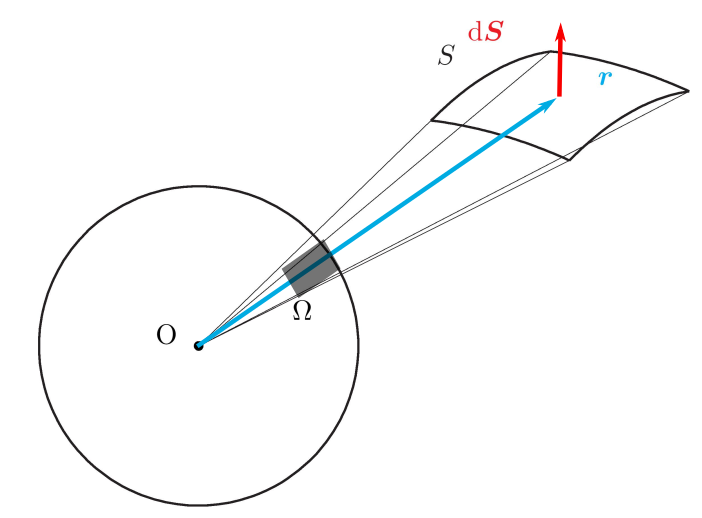
\includegraphics[width=7cm]{picture/steradian}
 \caption{立体角}
\label{fig:steradian}
\end{figure}

問題は,この面積をいかにして求めるかである.
実は,$\Omega$は次のように求めることができる.
\begin{align}
\Omega = \int_S \frac{\bm{r} }{r^3} \cdot \mathrm{d} \bm{S}
\label{eq:ritaikaku}
\end{align}
積分の式を解釈するときには被積分関数を眺めるとよいのであった.
$\bm{r}$と$\mathrm{d}\bm{S}$のなす角を$\theta$とすれば,
\begin{align*}
\frac{\bm{r}}{r^3} \cdot \mathrm{d} \bm{S} = \frac{1}{r^2} \, \mathrm{d} S \cos \theta
\end{align*}
である.
$\mathrm{d}S \cos\theta$という項について考えよう.
そもそも$\mathrm{d}S$というのは,位置$\bm{r}$における$S$の面素であり,
その意味は位置$\bm{r}$のごく近辺において$S$を平面とみなしたときの
その領域の面積であった.
それに$\cos \theta$をかけた量というのは,この領域を真上から角度
$\theta$だけずれた方向,つまり$\bm{r}$方向から眺めたときに
見える領域の面積を表している.
細かいことを考えなければこのことを示すのはあまり難しくはないから読者に任せておくことにしよう.

ここで,$S$を微小領域に分割したとき,各微小領域を$\bm{r}$方向から眺めた時に見える領域と
Oからその微小領域のふちに向かう各半直線と球面の交点として得られる領域
(図\ref{fig:steradian}の陰になっている部分)
は相似であって,その相似比は$1 : r$である.従ってその面積比は$1 : r^2$である.
よって,面積$\mathrm{d}S$の微小領域がつくる立体角$\mathrm{d} \Omega$は
\begin{align}
\mathrm{d} \Omega = \frac{1}{r^2} \, \mathrm{d} S \cos \theta
= \frac{\bm{r}}{r^3} \cdot \mathrm{d} \bm{S} 
\label{eq:bisyouomega}
\end{align}
となる.これを$S$全体にわたって足し合わせれば式(\ref{eq:ritaikaku})が得られることになる.

立体角の角度の単位はラジアンにならって
\emph{ステラジアン}\index[widx]{すてらじあん@ステラジアン}$[\mathrm{sr}]$
という単位が使われている.これもやはり無次元量である.

半径1の球面の表面積は$4 \pi$であるから,
任意の閉曲面$S_0$について,Oが$S_0$内部にある場合,
$S_0$のOに関する立体角は$4 \pi$ということになる.
しかしこれを式(\ref{eq:ritaikaku})に基づいて計算するのは少し面倒である.
また,Oが$S_0$外部にある場合,$S_0$のOに関する立体角は0になる.
これも式(\ref{eq:ritaikaku})に基づいて計算することはできるのだが,
ちょっと面倒なので本書では省略させてもらうことにする.


\section{微分演算子$\nabla$について}
電磁気学を学んでいるとよくこんなのが出てくる.
\begin{align}
\nabla = \left[
 \begin{array}{c}
\displaystyle
\frac{\partial}{\partial x} \\
\displaystyle
\frac{\partial}{\partial y} \\
\displaystyle
\frac{\partial}{\partial z} 
 \end{array}
\right] 
= \bm{e}_x \frac{\partial}{\partial x} + \bm{e}_y \frac{\partial}{\partial y} 
+ \bm{e}_z \frac{\partial}{\partial z}
\label{eq:nabla}
\end{align}
この記号$\nabla$は\emph{ナブラ}\index[widx]{なぶら@ナブラ($\nabla$)}と読む.
$\nabla$はベクトルとは言えないが,ベクトルっぽいものである.
よって手書きでは線を一本追加して二重文字で書く.
$\nabla$は微分演算子の一種であるとよく言われる.
$\nabla$は初学者キラーといっても過言ではないだろう.多くの人がこいつに苦しめられてきたにちがいない.
かくいう私もその1人である.だが,$\nabla$というのは単体ではまったく意味をなさない.
この記号を用いることで多くの式が簡便に,かつ統一的に表現できて便利だから使っているにすぎないのだ.
初学者の多くは$\nabla$単体の意味を必死に考え,そして挫折する.
だが,意味をもつのは$\nabla$単体ではなくそれを使って構成される種々の量である.
それを今から考えてみよう.
\subsection{微分演算子とは何か}
$\nabla$について考える前に,``演算子'',そして``微分演算子''というものについて考えてみよう.

それ単体では機能せず,他のものに対して何かしらの計算の指示を与えるものを
\emph{演算子}\index[widx]{えんざんし@演算子|textbf}という.数学者はよく``作用素''と呼んでいる.
``計算の指示''というと堅苦しく聞こえるかもしれないが,$\sin$とか$\ln$とか,
そんな感じのものが演算子である.
$\sin$や$\ln$というのは後ろのモノに対して
その正弦の値や自然対数
\footnote{自然対数というのは底が
Napire数$e$であるような対数のこと.数学では普通$\log$という記号で表すが,
数学以外では$\ln$と表すことが多い.}
の値を計算してくれ,という記号である.
和を表す記号$+$や積を表す記号$\times$も演算子の一種である.
また,演算子の中で後ろの関数を微分してくれ,という指示を含むような演算子のことを
\emph{微分演算子}\index[widx]{えんざんし@演算子!びぶん@微分---}という.
$\displaystyle \frac{\mathrm{d}}{\mathrm{d}x}$
や$\displaystyle \frac{\partial}{\partial x}$などは微分演算子である.

さらに,何かしらのモノに演算子をくっつけて実際に計算をさせることを演算子を\emph{作用させる}
\index[widx]{えんざんし@演算子!をさようさせる@---を作用させる}という.
なんだか偉そうに聞こえるが,大した言葉ではない.日常的にやっていることである.
例えば,数$x$の自然対数をとるという操作は``$x$に対して演算子$\ln$を作用させる''と言い換えることができるし,
$x, \, y$関数$f(x, \, y)$を$x$で偏微分するという操作は``関数$f$に微分演算子
$\displaystyle \frac{\partial}{\partial x}$を作用させる''
と言い換えることができる.言葉を言い換えるだけでなんだかとても高尚なことをやっている気分になる.
演算子というものに対してはそのくらいの気持ちで付き合っていけばいいのだ. 

演算子というものを考えると式を略記できることがある.例えば,
$$
\frac{\partial^2 f}{\partial x^2} + \frac{\partial^2 f}{\partial y^2} + \frac{\partial^2 f}{\partial z^2}
$$
という式があったときに,これは
$$
\left( \frac{\partial^2}{\partial x^2} + \frac{\partial^2}{\partial y^2} + \frac{\partial^2}{\partial z^2} \right) f
$$
と略記できる.この記法は式を簡潔に記述するだけでなく,式に隠れた対称性や規則性を浮き彫りにしてくれることがある.

\subsubsection{演算子は順番に気を付けろ}
使うのにはとっても便利な演算子であるが,
演算子は作用させる順番によって結果が変わることがある.
このことに気を付けないまま計算を進めた結果,なんだかよくわからないものが得られてしまったりするので気を付けなければならない.

例として微分演算子でやってみよう.微分演算子$\displaystyle \frac{\mathrm{d}}{\mathrm{d}x}$と
演算子としての関数$g$があったとする.関数$f$に$g$を作用させる,というのはその積$gf$をとれ
という計算をさせることだと解釈しておく.

まず,関数$f$に$\displaystyle \frac{\mathrm{d}}{\mathrm{d}x}$を作用させてから$g$を作用させてみる.
結果は
$$
g \left( \frac{\mathrm{d}f}{\mathrm{d}x} \right)  = g \frac{\mathrm{d}f}{\mathrm{d}x}
$$
となる.特に変わったところはない.

次に,$g$を作用させてから$\displaystyle \frac{\mathrm{d}}{\mathrm{d}x}$を作用させてみよう.
結果は
$$
\frac{\mathrm{d}}{\mathrm{d}x} (gf) = f \frac{\mathrm{d}g}{\mathrm{d}x} + g \frac{\mathrm{d}f}{\mathrm{d}x}
$$
となり,前者とは違った結果になってしまう.
演算子に関しては交換法則は成り立っていないのである.
座標変換などを考えるときにそういうことに出くわすことがあるだろう.
そのときになったら気を付けてもらえばいい.

\subsection{$\nabla$を使ってみよう}
演算子というのはそれ単体では大した意味を持たないことが多いというのはわかってもらえただろうか.
$\nabla$もそうである.$\nabla$単体の意味をどう解釈してみようか努力してみてもまったくの無駄である.
それよりも,$\nabla$を使って構成される量の方に興味があるのである.
本書ではスカラー場の勾配を表すグラーディエント,ベクトル場の発散を表すダイバージェンス,
そしてベクトル場の回転を表すローテーション(もしくはカール)の3つを学ぶ.

\subsection{スカラー場の勾配}
スカラー場$\phi(x, \, y, \, z)$があったとする.これに$\nabla$を作用させてベクトルを作ってみよう.
\begin{eqnarray}
\nabla \phi = \left[
 \begin{array}{c}
\displaystyle
\frac{\partial \phi}{\partial x} \\
\displaystyle
\frac{\partial \phi}{\partial y} \\
\displaystyle
\frac{\partial \phi}{\partial z} 
 \end{array}
\right]
\label{eq:gradnabla}
\end{eqnarray}
というベクトルができた.このベクトルをスカラー場$\phi$の\emph{勾配}
\index[widx]{すからーば@スカラー場!のこうばい@---の勾配}という.
このベクトルは,各点$(x, \, y, \, z)$に対し,$\phi$が最も急激に増加するような方向を指し示している.
そういうわけで``勾配''などといういかつい名前がついているのである.
と言われても,この式を見せられただけで納得できるような人はまずいない.
しかし,ちょっと考えればすぐにわかるのである.

$\phi$の全微分は
$$
\mathrm{d} \phi = \frac{\partial \phi}{\partial x} \mathrm{d} x 
+ \frac{\partial \phi}{\partial y} \mathrm{d} y +  \frac{\partial \phi}{\partial z} \mathrm{d} z
$$
であった.よく見ると,$\phi$の全微分$\mathrm{d}\phi$は位置の微小変化$\mathrm{d}\bm{r}$と
$\phi$の勾配$\nabla \phi$の内積になっているではないか.
つまり,$\phi$の微小変化$\mathrm{d}\phi$は位置の微小変化$\mathrm{d}\bm{r}$が
$\nabla \phi$の方向を向いているときに最も大きくなるのである.
こうしてみると,``勾配''というネーミングにも納得である.

また,``勾配''は英語ではgradientという.そういうわけで,スカラー場$\phi$の勾配を
\begin{eqnarray}
\mathrm{grad} \, \phi = \left[
 \begin{array}{c}
\displaystyle
\frac{\partial \phi}{\partial x} \\
\displaystyle
\frac{\partial \phi}{\partial y} \\
\displaystyle
\frac{\partial \phi}{\partial z} 
 \end{array}
\right]
\label{eq:gradgrad}
\end{eqnarray}
というように表す流儀もある.好きな方を使えばいいが,どちらの記号が出てきても混乱しないようにはしておくべきだ.

スカラー関数$\phi$について,$\nabla \phi$はベクトル場であった.
このベクトル場$\nabla \phi$を曲線$C$に沿って線積分することを考えよう.
$C$の始点,終点をそれぞれ$\bm{r}_A, \, \bm{r}_B$と表す.
\begin{align*}
\int_C \nabla \phi \cdot \mathrm{d}\bm{s} 
= \int_{\bm{r}_A}^{\bm{r}_B} \mathrm{d} \phi = \phi (\bm{r}_B) - \phi (\bm{r}_A) 
\end{align*}
となる.この計算はあえてノーヒントでいさせてもらおう.ヒントは本書の各所に散らばっている.
ここまできちんと学習を進めてこられたのであれば決して難しくないはずだ.

$\nabla \phi$の線積分は積分経路に依存せず,始点と終点にのみ依存するというわけだ.
すなわち,もしベクトル場$\bm{A}(\bm{r})$を$\bm{A}(\bm{r})=\nabla \phi$
と定めたのであれば,$\bm{A}(\bm{r})$は渦なし場であることがわかる.

\subsection{ベクトル場の発散}
$\nabla$はベクトルっぽいものであった.であれば,ベクトル場$\bm{A}(\bm{r})$について,
$\bm{A}(\bm{r})$と$\nabla$の内積を考えることができるだろう.そしてそれは
\begin{eqnarray}
\nabla \cdot \bm{A} (\bm{r}) =  \frac{\partial A_x}{\partial x} + \frac{\partial A_y}{\partial y} +  \frac{\partial A_z}{\partial z}
\label{eq:divnabla}
\end{eqnarray}
と書き表されるだろう.ベクトル場から1つのスカラーを得た.
これをベクトル場$\bm{A}(\bm{r})$の\emph{発散}\index[widx]{べくとるば@ベクトル場!のはっさん@---の発散}という.
この量は各点$(x, \, y, \, z)$に対し,その地点からベクトル場$\bm{A}(\bm{r})$がどれだけ湧き出しているかを表している.
そういうわけでこの量は発散と呼ばれているのである.全微分と似ているが,ちょっと違う.
微分されているのは$\bm{A}(\bm{r})$自身ではなく,その各成分である.

$x, \, y, \, z$のうち$x$だけが微小量$\mathrm{d}x$だけ変化したとき,$A_x$の微分$\mathrm{d} A_x$は
$$
\mathrm{d} A_x = \frac{\partial A_x}{\partial x} \mathrm{d}x
$$
と表されるのだった.
同様にして,$y$だけが微小量$\mathrm{d}y$だけ変化したとき,$A_y$の微分$\mathrm{d} A_y$は
$$
\mathrm{d} A_y = \frac{\partial A_y}{\partial y} \mathrm{d}y
$$
と表されるし,$z$だけが微小量$\mathrm{d}z$だけ変化したとき,$A_z$の微分$\mathrm{d} A_z$は
$$
\mathrm{d} A_z = \frac{\partial A_z}{\partial z} \mathrm{d}z
$$
と表される.この式に対して疑問がわくようであれば,再度偏微分のところの解説か,常微分の解説に戻っていただきたい.

もし$x$が増加して$A_x$が増加すれば,
それはその場所からベクトル場の$x$成分が湧いて出てきたと考えるほかはない.
``$x$が増加した''を``ある点よりも$x$軸方向に進んだ点を見た''と言い換えてみるとわかりやすいかもしれない.
ほかの成分に関しても同様である.$x$が変化したときに$\bm{A}(\bm{r})$の$y$成分や$z$成分の変化を考えないのは,
たとえ$y$成分や$z$成分が変化したとしても,
それはベクトル場の$y$成分や$z$成分が湧いて出てきたと考えることはできないからである.
各自図を描いて確認してほしい.こういうことには大いに悩むべきである.

式(\ref{eq:divnabla})は各軸方向の発散の総和である.
たとえ$x$軸の方向にベクトル場が湧き出していたとしても,
同じくらい$y$軸方向にベクトル場の吸い込みが発生していたとするならば,
それはベクトル場の発散があるというべきではないだろう.和をとっているのはそういう意味である.

``発散''は英語でdivergenceという.そんなわけで,ベクトル場の発散を$\nabla$を使わずに
\begin{eqnarray}
\mathrm{div} \, \bm{A}(\bm{r}) = \frac{\partial A_x}{\partial x} + \frac{\partial A_y}{\partial y} +  \frac{\partial A_z}{\partial z}
\label{eq:divdiv}
\end{eqnarray}
と表記することもある.これも好きな方を使うといい.
どちらの書き方が使われていてもきちんと読めるようにしておこう.

\subsection{\textrm{Gauss}の定理}
さて,$\mathrm{div} \, \bm{A}(\bm{r})$は各点$(x, \, y, \, z)$におけるベクトル場の発散を表しているのだった.
ところが,ベクトル場の発散といえば閉曲面上でベクトル場を面積分することでも得られたはずだ.

閉曲面上でベクトル場を面積分することで得られたのは,その閉曲面の内側から外側へのベクトル場の発散の合計であった.
一方,$\mathrm{div}\bm{A}(\bm{r})$が表すのは各点$(x, \, y, \, z)$での発散である.
これを閉曲面$S_0$の内部全体にわたって足し合わせれば,$S_0$の内側から外側への発散の合計が得られるはずだ.
積分領域は3次元領域であるから,これを$V$と表記しておこう.
この積分は,$V$を細かいさいころのようなブロックに分割して足し合わせていくイメージである. 
すると,次のような等式が成り立っているはずだ.
\begin{eqnarray}
\int_V \mathrm{div} \, \bm{A}(\bm{r}) \, \mathrm{d}V = \oint_{S_0} \bm{A}(\bm{r}) \cdot \mathrm{d}\bm{S}
\label{eq:Gaussthe}
\end{eqnarray}
ただし,$V$は$S_0$内部全体であり,右辺の面積分の向きは
$S_0$の内部から外部に向かうような向きであるとする.
式(\ref{eq:Gaussthe})を\textbf{Gaussの定理}\index[widx]{Gaussのていり@Gaussの定理}
\index[nidx]{Gauss@Gauss(ガウス)}と呼ぶ.
詳しい導出はやらない.その代わり式の解釈をしておこう.式(\ref{eq:Gaussthe})の両辺をよく眺めてほしい.
左辺の積分領域は$V$,つまり3次元領域で,右辺の積分領域は$S_0$,つまり2次元領域である.
Gaussの定理を利用するときにはこの性質をうまく利用することが多い.
つまり,Gaussの定理は積分領域を変更したいときに使われるのである.
たとえば,Maxwell\index[nidx]{Maxwell@Maxwell(マクスウェル)}
方程式を微分形から積分形,もしくはその逆に変形するときにこの定理は使われる.

とはいえ,いま理解すべきは左辺と右辺がともにベクトル場の発散を表しているということだ.
それさえ納得できてしまえば式(\ref{eq:Gaussthe})を忘れることもないだろう.
\subsection{ベクトル場の回転}
さっきやったのは$\nabla$とベクトルの内積である.今度は$\nabla$とベクトルの外積を考えてみよう.
何も考えずに計算してみれば,このようなベクトルが得られるはずだ.
\begin{eqnarray}
\nabla \times \bm{A}(\bm{r}) = \left[
\begin{array}{c}
\displaystyle
\frac{\partial A_z}{\partial y} - \frac{\partial A_y}{\partial z} \\
\displaystyle
\frac{\partial A_x}{\partial z} - \frac{\partial A_z}{\partial x} \\
\displaystyle
\frac{\partial A_y}{\partial x} - \frac{\partial A_x}{\partial y} 
\end{array}
\right]
\label{eq:rotnabla}
\end{eqnarray}
ベクトルの外積の成分表示のところをじっくり見ながら計算してみてほしい.
ベクトル場からまた違うベクトルを得た.これをベクトル場$\bm{A}(\bm{r})$の
\emph{回転}\index[widx]{べくとるば@ベクトル場!のかいてん@---の回転}という.このベクトルは各点$(x, \, y, \, z)$に対し,
その地点でベクトル場$\bm{A}(\bm{r})$がどの方向にどれだけの渦を巻いているかを表すベクトルである.
このベクトルが``回転''と呼ばれているのはそこからきている.
回転といってもいろいろな方向が考えられるだろう.
ベクトル場の回転がまたベクトルになっているのはそういうことである.
ベクトル場がどの向きに渦を巻いているかをしているかをそのベクトル場の回転の向きで,
渦がどの程度の強さなのかをそのベクトル場の回転のノルムによって表しているのである.

いま何を言っているかよくわからない人は,おそらく力学で回転関係の話を
学んでいないか,もしくはきちんと数学的に定式化された形で学んでいないかのどちらかだろう.
そういう人は多いだろうから,ざっくりとだが復習しておこう.
\subsubsection{回転を1本のベクトルで表す}
1本ベクトルが持っている方向というのは1つである.これはまったく当たり前のことである.
これだけで``回転''を表現するのは不可能に見えるかもしれない.
川の流れがぐるぐると渦を巻いている様子を想像してみると,それぞれの点では流れの向きはばらばらである.
しかし,全体を見てみるとなんとなく渦を巻いている.そんなイメージである.
この川の渦をたった1本のベクトルで表したい.
それにはどうすればよいだろうか? 必要なのは回転軸という考え方である.

ベクトルの外積のところで``2つのベクトル$\bm{a}, \, \bm{b}$について,
その外積$\bm{a} \times \bm{b}$の向きは,$\bm{a}$から$\bm{b}$の向きに右ネジを回したとき,
そのネジが進む方向であると定義する''と説明したのを覚えているだろうか.
あの場面では先にネジが回転する方向がわかり,それをもとに外積の向きが決まったのであった.
そう,回転の向きとベクトルの向きが対応しているのである.

逆に考えることはできないだろうか? ベクトルの向きが回転の方向を決めていると考えるのである.
それには``こういうベクトルにはこういう回転が対応しますよ''という約束事を指定しなくてはならない.
どうせなら外積と同じにしてしまおう.
あるベクトルが表す回転の向きは,そのベクトルの向きが右ネジが進む向きになるような
ネジの回転方向であると約束することにする.
回りくどい言い方だが,要はベクトルの外積のときと同じ対応関係になるようにしたのである.
ベクトルの大きさは,回転の強さを表すことにしておこう.これは自然な考えである.
大きさが大きいベクトルほどそのベクトルが表す回転は激しいのである.

これで1本のベクトルと1つの回転が完全に対応付けられた.
勘違いしてほしくないのだが,これはすべてのベクトルが回転を表すと決めたわけではない.
もしこのベクトルが回転を表すとしたら,それはこういう回転方向と強さを表していますよ,
というように約束事を作っただけである.
力$\bm{F}$が回転を表しているわけなかろう? そんなニュアンスである.

力学においてはこの約束事のもと,回転に関する種々の物理量がベクトル化される.
力のモーメント$\bm{N}$や角速度$\bm{\omega}$などである.
このようにベクトルで表しておくと,いろいろな方向の回転に対して式を統一的に表現できて便利である.
基準点からみて位置$\bm{r}$にある物体に力$\bm{F}$がはたらいているとき,
その力のモーメントは$\bm{N}=\bm{r}\times\bm{F}$と書き表され,
物体の角速度が$\bm{\omega}$であればその速度は$\bm{v}=\bm{\omega}\times\bm{r}$
と書き表される.

もし外積の順序を逆にしてしまうと,ベクトルの向きと回転方向の対応関係が崩れてしまう.
ベクトルの向きと回転方向の向きの対応関係は,人間が式を読み解くときに使うもので,
式そのものの中に回転方向が内蔵されているわけではないのである.
たとえば角速度$\bm{\omega}$がいくら回転を表しているといっても,
$\bm{\omega}$自体はただのベクトルである.
$\bm{\omega}$の向きは回転軸の方向を表していて,$\bm{\omega}$の大きさは回転の激しさを表している.
これが約束した正しい方向の回転を表すように仕向けるためには,
作った公式がうまく自身の方向と回転方向との関係を反映したものでなくてはならない.
角速度$\bm{\omega}$の例でいえば,$\bm{v}=\bm{\omega}\times\bm{r}$という式がそれである.

\begin{itembox}[l]{検討}
いまの話では,回転という現象をたった1本のベクトルで表せることを学んだ.
``回転''と``渦''はほぼ同じ意味だと思ってもらって構わない.
川に渦が巻いている状況を考えよう.渦であるからそれはベクトルで表せるはずだ.
しかし,川の渦は場所によって強さが違う.向きさえ一定ではないだろう.

このような状況では,この川の渦をたった1本の定まったベクトルとして表すのは不可能である.
いったいどうしたらいいだろう?
\end{itembox}

\subsubsection{ベクトル場の回転について考える}
ちょっと(しかし重要な)脱線をしたところで,話を戻そう.ベクトル場の回転というのは次の式で定義されるのだった.
\begin{eqnarray}
\nabla \times \bm{A}(\bm{r}) = \left[
\begin{array}{c}
\displaystyle
\frac{\partial A_z}{\partial y} - \frac{\partial A_y}{\partial z} \\
\displaystyle
\frac{\partial A_x}{\partial z} - \frac{\partial A_z}{\partial x} \\
\displaystyle
\frac{\partial A_y}{\partial x} - \frac{\partial A_x}{\partial y} 
\end{array}
\right]
\label{eq:rotnabla2}
\end{eqnarray}
このベクトルがベクトル場$\bm{A}(\bm{r})$の回転を表しているというのであった.
このことについて,少し考えてみよう.とはいえ,成分が3つあるので,まずは$z$成分から考えてみることにする.
なぜ$z$成分から考えるかというと,$\nabla \times \bm{A}(\bm{r})$の$z$成分が$\bm{A}(\bm{r})$の
$xy$平面内の回転を表しているからである.
このことについて考えてみる.

$\nabla \times \bm{A}(\bm{r})$の$z$成分は
\begin{eqnarray}
(\nabla \times \bm{A}(\bm{r}))_z = \frac{\partial A_y}{\partial x} - \frac{\partial A_x}{\partial y} 
\label{eq:rotnablaz}
\end{eqnarray}
である.ベクトルの成分を表すのに,そのベクトルに対応する成分を表す添え字をつけることがある.
こういう表記は大概予告なしに使われることがあるので覚えておこう.

さて,式(\ref{eq:rotnablaz})が何を表しているのか考えてみよう.
まずは第1項
$$
\frac{\partial A_y}{\partial x}
$$
からである.この項は$x$が変化したときの$\bm{A}(\bm{r})$の$y$成分の変化率を表しているのだった.
もしこの項が正であれば,それは$x$軸の正方向に進めば進むほど$\bm{A}(\bm{r})$の$y$成分が増加していくことになる.

第2項
$$
-\frac{\partial A_x}{\partial y}
$$
についても同じように考えてやる.この項は$y$が変化したときの$\bm{A}(\bm{r})$の$x$成分の変化率を表している.
頭に$-$記号がくっついているので,
この項が全体として正であるときには
$y$軸の正方向に進めば進むほど,$\bm{A}(\bm{r})$の$x$成分が減少していくことになる.

すなわち,$x$に対して$\bm{A}(\bm{r})$の$y$成分が増加し,かつ$y$に対して$\bm{A}(\bm{r})$の$x$成分が減少するとき,
$\nabla \times \bm{A}(\bm{r})$の$z$成分は大きな値をとる.
このような場合,$\bm{A}(r)$の分布はどうなっているだろうか? 図に書き起こしてみよう.
\begin{figure}[h]
 \begin{minipage}{0.5\hsize}
  \begin{center}
   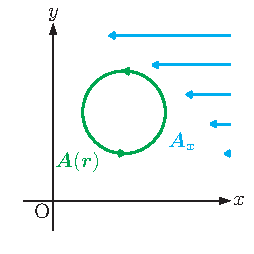
\includegraphics[width=5cm]{picture/vecterana5}
  \end{center}
 \caption{ベクトル場の回転その1}
 \label{fig:vecrot1}
\end{minipage}
\begin{minipage}{0.5\hsize}
  \begin{center}
   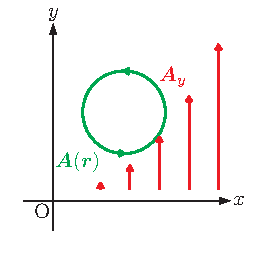
\includegraphics[width=5cm]{picture/vecterana6}
  \end{center}
 \caption{ベクトル場の回転その2}
 \label{fig:vecrot2}
\end{minipage}
\end{figure} \\

$A_x$と$A_y$の分布を見たときに,
$\bm{A}(\bm{r})$の渦のようなものが見えてくる.
$xy$平面を川だと思い,$\bm{A}(\bm{r})$を川の流れを表すベクトル場だと思ってみる.
そして,この川の緑色の円の中心あたりに水車があると思ってみよう.
水車は図の緑の矢印のような向きに回転するはずだ.


$xy$平面に反時計回りの渦が発生しているとき,これを右ネジが回転する方向だと思うことにすると,
右ネジは$z$軸正方向を進むことになる.
したがって,この渦を表すベクトルは$z$軸正方向を向いているべきである.
また,図を見る限り,$A_x$と$A_y$の変化が激しいほど強い渦が発生していることになるだろう.
これらのことから察するに,この渦を表しているのは$\nabla \times \bm{A}(\bm{r})$の$z$成分である.
すなわち,$\nabla \times \bm{A}(\bm{r})$の$z$成分は
ベクトル場$\bm{A}(\bm{r})$の$xy$平面上にある渦の向きと強さを表しているのである.
もしも$\nabla \times \bm{A}(\bm{r})$の$z$成分が負であれば,
それはベクトル場$\bm{A}(\bm{r})$の$xy$平面上にある渦の向きが
図と逆向きであるということだ.

と書いてみたものの,
これは$\nabla \times \bm{A}(\bm{r})$が$\bm{A}(\bm{r})$の回転を表していることを無理やりにでも納得してもらうための
都合のいい例を出したにすぎない.
実際のベクトル場はもっと複雑で,どう見ても渦には見えないようなベクトル場であってもそれとナブラとの外積をとってみると
$\bm{0}$にはなってくれないことがしょっちゅうある.そういうときは定義式を眺めてそんなものかと納得しておけばよい.
人間の勝手な思い込みなどさっさと捨て去ってしまうべきだ.
\begin{itembox}[l]{課題}
上の考察にならって,$\nabla \times \bm{A}(\bm{r})$の$x$成分や$y$成分が何を表しているかを調べよ.
\end{itembox}

$\nabla \times \bm{A}(\bm{r})$が$\bm{A}(\bm{r})$の回転を表していることは理解できただろう.
そういうわけで,ベクトル場の回転を英単語rotationやcurlからとって
\begin{eqnarray}
\mathrm{rot} \, \bm{A}(\bm{r}) = \left[
\begin{array}{c}
\displaystyle
\frac{\partial A_z}{\partial y} - \frac{\partial A_y}{\partial z} \\
\displaystyle
\frac{\partial A_x}{\partial z} - \frac{\partial A_z}{\partial x} \\
\displaystyle
\frac{\partial A_y}{\partial x} - \frac{\partial A_x}{\partial y} 
\end{array}
\right]
\label{eq:rotrot}
\end{eqnarray}
だったり,
\begin{eqnarray}
\mathrm{curl} \, \bm{A}(\bm{r}) = \left[
\begin{array}{c}
\displaystyle
\frac{\partial A_z}{\partial y} - \frac{\partial A_y}{\partial z} \\
\displaystyle
\frac{\partial A_x}{\partial z} - \frac{\partial A_z}{\partial x} \\
\displaystyle
\frac{\partial A_y}{\partial x} - \frac{\partial A_x}{\partial y} 
\end{array}
\right]
\label{eq:rotcurl}
\end{eqnarray}
というように表すことがある.rot表記は主に日本で,curl表記は主に海外で用いられることが多いようである.
好きなものを採用すればいいが,やはりどれが出てきても混乱しないようにはしておこう.

\subsection{\textrm{ Stokes}の定理}
$\mathrm{rot} \, \bm{A}(\bm{r})$はベクトル場$\bm{A}(\bm{r})$の回転を表すのだった.
回転を表すといっても,$\mathrm{rot} \, \bm{A}(\bm{r})$はベクトル場で,
$\bm{A}(\bm{r})$の各点$(x, \, y, \, z)$における局所的な回転を表している.
これをある曲面$S$上全体にわたって面積分したらどうなるだろうか? ベクトル場の面積分が表しているのは
ベクトル場がその曲面を垂直に貫くような場の分布であった.
いま積分するのは$\bm{A}(\bm{r})$自身ではなく$\mathrm{rot} \, \bm{A}(\bm{r})$である.
$\mathrm{rot} \, \bm{A}(\bm{r})$が曲面を垂直に貫いているような分布がどれだけあるかを計算するということは,
すなわちもとのベクトル場がその曲面にそってどのくらいの強さの渦を巻いているかを計算しているのと
同じことである.従って,曲面$S$のふちを$C_0$とすれば,$C_0$はもちろん閉曲線で
\begin{eqnarray}
\int_S \mathrm{rot} \, \bm{A}(\bm{r}) \cdot \mathrm{d} \bm{S} =
\oint_{C_0} \bm{A}(\bm{r}) \cdot \mathrm{d}\bm{s}
\label{eq:Stokesthe}
\end{eqnarray}
という式が成り立っているということが推測できる.ただし,$S$は空間にある任意の曲面で,
$C_0$はそのふちである.
ただし,曲面$S$の向きは$C_0$に沿って曲面のふちを1周するとき,
その向きに右ネジを回したときにネジが進むような向きであるとする.

実際,式(\ref{eq:Stokesthe})は厳密に成り立っていて,
\textbf{Stokesの定理}\index[widx]{Stokesのていり@Stokesの定理}
\index[nidx]{Stokes@Stokes(ストークス)}と呼ばれている.
Gaussの定理とよく似た形をした等式である.あちらと合わせて頭に叩き込んでしまおう.

この式もGaussの定理と同じく,線積分を面積分に変換したり,またその逆を行ったりするときによく使われる.
だが,とりあえず今確認すべきなのは,
式(\ref{eq:Stokesthe})の両辺がともに$\bm{A}(\bm{r})$の回転を表しているということである.

\subsection{ベクトル場のポテンシャル}
Gaussの定理やStokesの定理を学んだところで,
どうやらベクトル場の閉じた領域での積分は
そのベクトル場の発散や回転に関係しているらしいというのが見えてきたのであった.
そのあたりについてもう少し詳しく話しておこう.

まずは渦なし場について考えよう.ベクトル場$\bm{A}(\bm{r})$が渦なし場であるというのは,
任意の閉曲線に沿った周回積分が0になるようなベクトル場であった.
渦なし場$\bm{A}(\bm{r})$では$\mathrm{rot} \, \bm{A}(\bm{r}) = \bm{0}$
が常に成り立つ.Stokesの定理とにらめっこしていればすぐにわかるから,
いちいち解説する必要性は感じない.

また,渦なし場に対してはスカラーポテンシャルなる量が定義できるのであった.
以前は渦なし場の線積分としてスカラーポテンシャルを定義したが,
通常``ベクトル場$\bm{A}(\bm{r})$について,$\bm{A}(\bm{r}) = - \nabla \phi (\bm{r})$なる
スカラー関数$\phi(\bm{r})$が存在するとき,この$\phi (\bm{r})$を$\bm{A}(\bm{r})$のスカラーポテンシャルと呼ぶ''
\index[widx]{すからー@スカラー!ぽてんしゃる@---ポテンシャル}
というように定義するのが普通である.
もちろん,この2つの定義はまったく同じ定義であり,
どちらの定義を採用しても構わない.
このことを確認するためのヒントは本書のいたるところに散らばっている.
\begin{itembox}[l]{定理}
ベクトル場$\bm{A}(\bm{r})$について,以下の条件はすべて同値である.
\begin{enumerate}
\item $\mathrm{rot} \, \bm{A}(\bm{r})=\bm{0}$が常に成り立つ.
\item $\bm{A}(\bm{r}) = - \nabla \phi(\bm{r})$なるスカラー関数$\phi(\bm{r})$が存在する.
\item 任意の閉曲線$C_0$に対し,$C_0$に沿った$\bm{A}(\bm{r})$の周回積分が0になる.
\end{enumerate}
\end{itembox}
きちんと証明をしたわけではないが,これまで学んできた事項を整理してやればこうなるのである.
渦なし場については以上のような特徴づけができた.
閉曲線に沿った周回積分と$\mathrm{rot}$,
そしてスカラーポテンシャルは表裏一体の関係にあるのである.

当然次は閉曲面上での面積分と$\mathrm{div}$の関係が気になるところである.
これに関しても同じような特徴づけができることが知られている.
詳しい説明はしないが結果だけ述べておく.
\begin{itembox}[l]{定理}
ベクトル場$\bm{A}(\bm{r})$について,以下の条件はすべて同値である.
\begin{enumerate}
\item $\mathrm{div} \, \bm{A}(\bm{r})=0$が常に成り立つ.
\item $\bm{A}(\bm{r}) = \nabla \times \bm{B} (\bm{r})$なるベクトル場$\bm{B}(\bm{r})$が存在する.
\item 任意の閉曲面$S_0$に対し,$S_0$上での$\bm{A}(\bm{r})$の面積分が0になる.
\end{enumerate}
\end{itembox}
非常に対称的な関係である.ベクトル場$\bm{A}(\bm{r})$について,
$\bm{A}(\bm{r}) = \nabla \times \bm{B}(\bm{r})$なるベクトル場$\bm{B}(\bm{r})$が存在するとき,
この$\bm{B}(\bm{r})$を$\bm{A}(\bm{r})$の\emph{ベクトルポテンシャル}
\index[widx]{べくとる@ベクトル!ぽてんしゃる@---ポテンシャル}と呼ぶ.
スカラーポテンシャルに対してベクトルポテンシャル,実に対称的で美しいネーミングである.

ここまでは発散のないベクトル場,回転(渦)のないベクトル場について考えてきたが,
一般のベクトル場について考えるのであれば,発散も回転もあるのが普通である.
ところが,先に述べた2つの定理を組み合わせたような主張が成り立つことが知られている.
\begin{itembox}[l]{Helmholtzの定理}
ベクトル場$\bm{A}(\bm{r})$について,$\bm{A}(\bm{r})$が無限遠において十分速く$\bm{0}$
に収束するとき,スカラー関数$\phi ( \bm{r})$とベクトル場$\bm{B}(\bm{r})$
が存在して
\begin{align}
\bm{A}(\bm{r}) = - \nabla \phi (\bm{r} ) + \nabla \times \bm{B}(\bm{r})
\label{eq:helmholtz}
\end{align}
が成り立つ.
\end{itembox}
この定理は\textbf{Helmholtzの定理}\index[widx]{Helmholtzのていり@Helmholtzの定理},
\index[nidx]{Helmholtz@Helmholtz(ヘルムホルツ)}
もしくは\emph{ベクトル解析の基本定理}\index[widx]{べくとるかいせきのきほんていり@ベクトル解析の基本定理|see{Helmholtzの定理}}
と呼ばれる非常に重要な定理である.例によって証明はしないが定理の主張は
頭に叩き込んでおきたいものである.

\subsection{ラプラシアン}
ベクトル場の発散と回転は,ベクトルとナブラの内積,および外積を実行することで得られるのであった.
ではナブラ同士ではどうだろうか? 演算子同士を組み合わせて新しい演算子を作り出すというのはよくやることである.
ナブラ同士の外積は結果が美しくならなそうなので内積をやってみよう.
特に何も考えずにやってみると,
\begin{align}
\nabla \cdot \nabla = \frac{\partial^2}{\partial x^2} + \frac{\partial^2}{\partial y^2} + \frac{\partial^2}{\partial z^2}
\label{eq:lap}
\end{align}
とまあなんとなくきれいな感じになる.こういう形の式は物理をやっているといたるところで出てくる.
よく出てくるのだから1文字で表して特別な名前をつけてやろう.
式(\ref{eq:lap})に出てきた演算子を\emph{ラプラシアン}
\index[widx]{らぷらしあん@ラプラシアン($\bigtriangleup$)}と呼び,
記号$\bigtriangleup$で表す.
\begin{align}
\bigtriangleup = \frac{\partial^2}{\partial x^2} + \frac{\partial^2}{\partial y^2} + \frac{\partial^2}{\partial z^2}
\label{eq:Lap}
\end{align}
と定めるのである.式(\ref{eq:lap})を見る限り,ラプラシアンは$\nabla^2$と書いてもいい気がする.
いや,ナブラとそれ自身との内積を求めたのだから$| \nabla |^2$と表すべきだろうか? ただ,
$| \nabla |^2$というのは書くのが面倒だし$\nabla^2$にしておくことにしよう.
今は記号の使い方を定義する場面なのでこういうことができるのだ.式(\ref{eq:lap})を導くのにやった計算は
内積の計算のようなものだが,$\nabla$というのはそもそもベクトルではなくあくまでベクトルっぽいものなのだった.
まとめると,$\bigtriangleup$と$\nabla^2$はまったく同じ意味で,それは式(\ref{eq:Lap})の右辺にある演算子を表している.

なお,$\bigtriangleup$を手書きで書くとき,人によって2重文字にしたりしなかったりする.
ラプラシアンはスカラーっぽいので普通のスカラー量を表すときのようにそのまま三角を書くのも納得である.
しかし,普通に三角で書かれると,もはやギリシャ文字$\Delta$と区別がつかない.
そういうわけで2重文字で書く人もいる.
もっとも,ワープロで打つときもラプラシアンをギリシャ文字$\Delta$で表してしまっていることも多い.
試しにネットで検索してみたらそういうサイトはたくさんあった.
文脈によって書いてある``$\Delta$''がギリシャ文字$\Delta$なのか,
それともラプラシアン$\bigtriangleup$なのかを見分けなくちゃいけないのはなかなか面倒である.
そういうわけで,読者の方々にはラプラシアンは2重文字で書くのを勧めておく.

ラプラシアンはスカラーにでもベクトルにでも作用させることができる.
スカラー関数$\phi$に対しては
\begin{align}
\bigtriangleup \phi = \frac{\partial^2\phi}{\partial x^2} + 
\frac{\partial^2 \phi}{\partial y^2} + \frac{\partial^2 \phi}{\partial z^2}
\label{eqsclap}
\end{align}
というようにラプラシアンを作用させて新しいスカラー関数ができて,ベクトル$\bm{A}$に対しては
\begin{align}
\bigtriangleup \bm{A} = \frac{\partial^2 \bm{A} }{\partial x^2} + 
\frac{\partial^2 \bm{A} }{\partial y^2} + \frac{\partial^2 \bm{A} }{\partial z^2}
\label{eq:veclap}
\end{align}
というようにラプラシアンを作用させて新しいベクトルを作り出すことができる.

$\bigtriangleup \phi$や$\bigtriangleup \bm{A} $がそれぞれ何を表しているかとか,
考えられなくもないが,$\mathrm{div}$や$\mathrm{rot}$のときほど重要な話でもない.
ただなんとなくラプラシアンという演算子があるんだなあとでも思っておけばよいだろう.

注意点として,ラプラシアン$\bigtriangleup$はスカラー関数に作用させる文脈においては演算子$\mathrm{div \, grad}$
とまったく同じ意味を持つが,ラプラシアンをベクトルに作用させる文脈においては$\mathrm{div \, grad}$
と書くべきではない.なぜだかわかるだろうか? スカラー関数$\phi$に対してその勾配$\mathrm{grad} \, \phi$を計算し,
さらにその発散をとるという計算はできるが,これがベクトルになると,
あるベクトル$\bm{A}$の勾配をとるなどという意味不明なことになってしまうからだ.
演算子同士の計算ではこういうことはけっこう起こるので注意しよう.迷ったときには作用させる対象も入れて計算するとよい.

\subsection{微分演算子同士の組み合わせ}
ラプラシアンのときにやったのはナブラとナブラの内積で,これはスカラー関数に作用させるときには
演算子$\mathrm{div \, grad}$と同じ意味を持つのであった.
では,他はどうだろう? 今のところ,$\mathrm{grad, \, div, \, rot}$と3種類ある.
これらをうまいこと組み合わせて何か面白い演算子が作れそうな気がする.
組み合わせのバリエーションは,演算子を作用させる順番によって結果が変わることを考慮すると
$3 \times 3 =9$通りだけありそうだが,実際に試してみると
\begin{align*}
&\mathrm{grad \, div} \\
&\mathrm{div \, grad} \\
&\mathrm{div \, rot} \\
&\mathrm{rot \, grad} \\
&\mathrm{rot \, rot} 
\end{align*}
の5種類しかない.どの演算子が何に作用して何を作るのかを理解していればわかるはずだ.
これをそれぞれ地道に計算してみると,$\mathrm{grad \, div}$に関しては面白い結果は出てこなくて,他のものは
\begin{align}
\mathrm{div \, grad} &= \bigtriangleup \\
\mathrm{div \, rot} &= 0 \\
\mathrm{rot \, grad} &= \bm{0} \\
\mathrm{rot \, rot} &= \mathrm{grad \, div} - \bigtriangleup
\end{align}
という結果になる.ただただ定義に従って地道に計算していくだけなのでいちいち書かなくてもいいだろう.
読者の方々の計算問題としておこう.

\section{微分演算子の座標変換}
微分演算子$\nabla$について学んできたが,
\begin{align*}
\nabla = \bm{e}_x \frac{ \partial}{\partial x} + \bm{e}_y \frac{ \partial}{\partial y}
+ \bm{e}_z \frac{ \partial}{\partial z}
\end{align*}
という書き方はDescartes座標系を基準にして考えていたのであった.
この量を他の座標系で表したいというのが今回のテーマである.
よく使うのが極座標系への変換なので,今回は極座標系への変換を行ってみる.

\subsection{$\nabla$の極座標変換}
さっきの話だけを聞くと,
\begin{align*}
\nabla = \bm{e}_r \frac{ \partial }{\partial r} + \bm{e}_{\theta}
 \frac{ \partial }{\partial \theta } 
 + \bm{e}_{\varphi} \frac{ \partial }{\partial \varphi} 
\end{align*}
と計算して話を終わりにしたくなるが,もちろん間違いである.
あくまで我々が求めたいのはDescartes座標系での$\nabla$を極座標系に変換したいのであって,
極座標系で$\nabla$という演算子を新しく定義したいのではないのである.
つまり,Descartes座標系において関数$f$に$\nabla$を作用させた量
\begin{align*}
\bm{e}_x \frac{ \partial f }{\partial x} + \bm{e}_y \frac{ \partial f } {\partial y}
+ \bm{e}_z \frac{ \partial f }{\partial z}
\end{align*}
が極座標系ではどのような形になるのかを求めたいのである.

そのために何をすべきかといえば,
要は$\bm{e}_x, \, \bm{e}_y, \, \bm{e}_z$と微分演算子を極座標系で表してやればいいのである.
基底ベクトルの方は,以前
\begin{align*}
\bm{e}_x & = & \sin \theta \cos \varphi \, \bm{e} _r & & 
+ \cos \theta \cos \varphi \, \bm{e}_\theta & & - \sin \varphi \, \bm{e}_\varphi & \\
\bm{e}_y & = & \sin \theta \sin \varphi \, \bm{e}_r & & 
+ \cos \theta \sin \varphi \, \bm{e}_\theta & & 
+ \cos \varphi \, \bm{e}_\varphi & \\
\bm{e}_z & = & \cos \theta \, \bm{e}_r & & - \sin \theta \, \bm{e}_\theta &
\end{align*}
という式が成り立つことを懇切丁寧に解説したのだった.
微分演算子の方も以前全微分の解説をしたときに
\begin{align*}
\frac{ \partial f} {\partial r} & 
= \frac{ \partial f} {\partial x} \frac{ \partial x} {\partial r}
+ \frac{ \partial f} {\partial y} \frac{ \partial y} {\partial r}
+ \frac{ \partial f} {\partial z} \frac{ \partial z} {\partial r} \\
\frac{ \partial f} {\partial \theta} & 
= \frac{ \partial f} {\partial x} \frac{ \partial x} {\partial \theta}
+ \frac{ \partial f} {\partial y} \frac{ \partial y} {\partial \theta}
+ \frac{ \partial f} {\partial z} \frac{ \partial z} {\partial \theta} \\
\frac{ \partial f} {\partial \varphi} & 
= \frac{ \partial f} {\partial x} \frac{ \partial x} {\partial \varphi}
+ \frac{ \partial f} {\partial y} \frac{ \partial y} {\partial \varphi}
+ \frac{ \partial f} {\partial z} \frac{ \partial z} {\partial \varphi} \\
\end{align*}
という式が成り立つことを紹介したのであった.
後はこれをいかにも連立方程式っぽく
\begin{align*}
\left[ 
\renewcommand{\arraystretch}{2}
\begin{array}{c}
\dfrac{ \partial f} {\partial r} \\
\dfrac{ \partial f} {\partial \theta} \\
\dfrac{ \partial f} {\partial \varphi}
\end{array}
\right] = \left[
\begin{array}{ccc}
\dfrac{ \partial x} {\partial r} & \dfrac{ \partial y} {\partial r} 
& \dfrac{ \partial z} {\partial r} \\
\dfrac{ \partial x} {\partial \theta} & \dfrac{ \partial y} {\partial \theta} 
& \dfrac{ \partial z} {\partial \theta} \\ 
\dfrac{ \partial x} {\partial \varphi} & \dfrac{ \partial y} {\partial \varphi}
& \dfrac{ \partial z} {\partial \varphi}
\end{array}
\right]
\left[
\begin{array}{c}
\dfrac{ \partial f} {\partial x} \\
\dfrac{ \partial f} {\partial y} \\
\dfrac{ \partial f} {\partial z}
\end{array}
\right]
\end{align*}
と書き表してやる.係数行列の偏微分を実際に求めてやると,
\begin{align*}
\left[ 
\renewcommand{\arraystretch}{2}
\begin{array}{c}
\dfrac{ \partial f} {\partial r} \\
\dfrac{ \partial f} {\partial \theta} \\
\dfrac{ \partial f} {\partial \varphi}
\end{array}
\right] = \left[
\renewcommand{\arraystretch}{1}
\begin{array}{ccc}
\sin \theta \cos \varphi & r \cos \theta \cos \varphi & - r \sin \theta \sin \varphi \\
\sin \theta \sin \varphi & r \cos \theta \sin \varphi & r \sin \theta \cos \varphi \\
\cos \theta & -r \sin \theta & 0
\end{array}
\right]
\left[
\renewcommand{\arraystretch}{2}
\begin{array}{c}
\dfrac{ \partial f} {\partial x} \\
\dfrac{ \partial f} {\partial y} \\
\dfrac{ \partial f} {\partial z}
\end{array}
\right]
\renewcommand{\arraystretch}{1}
\end{align*}
となる.どこかで見たことがあるような式である.あとは
連立方程式を解く要領で
$\dfrac{ \partial f} {\partial x} , \, \dfrac{ \partial f} {\partial y} , \, \dfrac{ \partial f} {\partial z}$
を求めてやればよい.
係数行列がヤコビ行列であることを思い出しつつ,
線形代数学の知識のフル稼働させて係数行列の逆行列を求めてやれば,
\begin{align*}
\left[
\renewcommand{\arraystretch}{2}
\begin{array}{c}
\dfrac{ \partial f} {\partial x} \\
\dfrac{ \partial f} {\partial y} \\
\dfrac{ \partial f} {\partial z}
\end{array}
\right] = \left[
\begin{array}{ccc}
\sin \theta \cos \varphi & \dfrac{ \cos \theta \cos \varphi}{r}
& - \dfrac{ \sin \varphi }{r \sin \theta } \\
\sin \theta \sin \varphi & \dfrac{ \cos \theta \sin \varphi}{r}
& \dfrac{ \cos \varphi }{r \sin \theta } \\
\cos \theta & - \dfrac{ \sin \theta }{r} & 0 
\end{array}
\right] \left[
\begin{array}{c}
\dfrac{ \partial f} {\partial r} \\
\dfrac{ \partial f} {\partial \theta} \\
\dfrac{ \partial f} {\partial \varphi}
\end{array}
\right] 
\end{align*}
となる.つまり,
\begin{align}
\begin{aligned}
\frac{ \partial f}{\partial x} & = & \sin \theta \cos \varphi & \frac{ \partial f}{\partial r}
& + \frac{ \cos \theta \cos \varphi }{r} & \frac{ \partial f}{\partial \theta} 
& - \frac{ \sin \varphi }{ r \sin \theta } &  \frac{ \partial f}{\partial \varphi} \\
\frac{ \partial f}{\partial y} & = & \sin \theta \sin \varphi & \frac{ \partial f}{\partial r}
& + \frac{ \cos \theta \sin \varphi }{r} &  \frac{ \partial f}{\partial \theta} 
& + \frac{ \cos \varphi }{ r \sin \theta } & \frac{ \partial f}{\partial \varphi} \\
\frac{ \partial f}{\partial z} & = & \cos \theta & \frac{ \partial f}{\partial r} 
& - \frac{ \sin \theta }{r} & \frac{ \partial f}{\partial \theta}
\end{aligned}
\label{eq:kyokuDesbibunhenkan}
\end{align}
ということである.関数$f$は任意だったから,結局演算子として
\begin{align}
\begin{aligned}
\frac{ \partial }{\partial x} & = & \sin \theta \cos \varphi & \frac{ \partial }{\partial r}
& + \frac{ \cos \theta \cos \varphi }{r} & \frac{ \partial }{\partial \theta} 
& - \frac{ \sin \varphi }{ r \sin \theta } &  \frac{ \partial }{\partial \varphi} \\
\frac{ \partial }{\partial y} & = & \sin \theta \sin \varphi & \frac{ \partial }{\partial r}
& + \frac{ \cos \theta \sin \varphi }{r} &  \frac{ \partial }{\partial \theta} 
& + \frac{ \cos \varphi }{ r \sin \theta } & \frac{ \partial }{\partial \varphi} \\
\frac{ \partial }{\partial z} & = & \cos \theta & \frac{ \partial }{\partial r} 
& - \frac{ \sin \theta }{r} & \frac{ \partial }{\partial \theta}
\end{aligned}
\label{eq:kyokuDesopehenkan}
\end{align}
という公式が得られたことになる.
演算子的な関係式に書き直したからには
もはや積の順番を勝手に入れ替えることは許されない.
式中にある$\sin \theta \cos \varphi$や$\dfrac{ \cos \varphi}{r \sin \theta}$
も演算子として扱わなければならないのである.

さらに話を進めよう.式(\ref{eq:kyokuDesopehenkan})をちょこっとだけ変形してやって
再度行列形式に書き直してやると
\begin{align}
\left[
\renewcommand{\arraystretch}{2}
\begin{array}{c}
\dfrac{ \partial } {\partial x} \\
\dfrac{ \partial } {\partial y} \\
\dfrac{ \partial } {\partial z}
\end{array}
\right] = \left[
\renewcommand{\arraystretch}{1}
\begin{array}{ccc}
\sin \theta \cos \varphi & \cos \theta \cos \varphi
& - \sin \varphi \\
\sin \theta \sin \varphi & \cos \theta \sin \varphi
& \cos \varphi \\
\cos \theta & - \sin \theta & 0 
\end{array}
\right] \left[
\begin{array}{c}
\dfrac{ \partial } {\partial r} \\
\dfrac{1}{r} \dfrac{ \partial } {\partial \theta} \\
\dfrac{1}{r \sin \theta } \dfrac{ \partial } {\partial \varphi}
\end{array}
\right] 
\label{eq:kyokuDesopehenkan2}
\end{align}
という式が得られる.計算を楽チンに進めるためにちょっとした小細工をしてみる.
我々はどこかでこんな式を見たことがあるとしよう.
\begin{align}
\renewcommand{\arraystretch}{1}
\left[
\begin{array}{ccc}
\bm{e}_x & \bm{e}_y & \bm{e}_z
\end{array}
\right]
= \left[
\begin{array}{ccc}
\bm{e}_r & \bm{e}_\theta & \bm{e}_\varphi 
\end{array}
\right]
\left[
\begin{array}{ccc} 
\sin \theta \cos \varphi & \sin \theta \sin \varphi & \cos \theta \\
\cos \theta \cos \varphi & \cos \theta \sin \varphi & - \sin \theta \\
- \sin \varphi & \cos \varphi & 0
\end{array}
\right]
\label{eq:kyokuDeskiteihenkanx}
\end{align}
行列の成分に共通点が多すぎる.というよりほぼ同じ行列である.
そこで,行列$A$を
\begin{align*}
A = \left[
\renewcommand{\arraystretch}{1}
\begin{array}{ccc} 
\sin \theta \cos \varphi & \sin \theta \sin \varphi & \cos \theta \\
\cos \theta \cos \varphi & \cos \theta \sin \varphi & - \sin \theta \\
- \sin \varphi & \cos \varphi & 0
\end{array}
\right]
\end{align*}
と定めると,式(\ref{eq:kyokuDesopehenkan2})は
$A$の転置行列${}^t \! A$を用いて
\begin{align*}
\left[
\renewcommand{\arraystretch}{2}
\begin{array}{c}
\dfrac{ \partial } {\partial x} \\
\dfrac{ \partial } {\partial y} \\
\dfrac{ \partial } {\partial z}
\end{array}
\right] = {}^t \! A 
\left[
\begin{array}{c}
\dfrac{ \partial } {\partial r} \\
\dfrac{1}{r} \dfrac{ \partial } {\partial \theta} \\
\dfrac{1}{r \sin \theta } \dfrac{ \partial } {\partial \varphi}
\end{array}
\right] 
\end{align*}
と表せて,式(\ref{eq:kyokuDeskiteihenkanx})の方は
\begin{align*}
\renewcommand{\arraystretch}{1}
\left[
\begin{array}{ccc}
\bm{e}_x & \bm{e}_y & \bm{e}_z
\end{array}
\right]
= \left[
\begin{array}{ccc}
\bm{e}_r & \bm{e}_\theta & \bm{e}_\varphi 
\end{array}
\right] A
\end{align*}
と書き換えられることになる.さらに読者が直交行列という言葉も耳にしており,
\begin{align*}
{}^t \! A A = A {}^t \! A = E \quad ( E\text{は単位行列})
\end{align*}
が成り立つことも知っていたとする.
もし知らないのなら線形代数学の教科書を見返してくるか,
とりあえずそのまま受け入れるかして先に進んでほしい.

これらの式を用いれば,$\nabla$が極座標を用いて書き下せて
\begin{align*}
\nabla & = \left[
\renewcommand{\arraystretch}{1}
\begin{array}{ccc}
\bm{e}_x & \bm{e}_y & \bm{e}_z 
\end{array}
\right] \left[
\renewcommand{\arraystretch}{2}
\begin{array}{c}
\dfrac{ \partial } {\partial x} \\
\dfrac{ \partial } {\partial y} \\
\dfrac{ \partial } {\partial z}
\end{array}
\right] \\
& = \left[
\renewcommand{\arraystretch}{1}
\begin{array}{ccc}
\bm{e}_r & \bm{e}_\theta & \bm{e}_\varphi 
\end{array}
\right] A  {}^t \! A 
\left[
\renewcommand{\arraystretch}{2}
\begin{array}{c}
\dfrac{ \partial } {\partial r} \\
\dfrac{1}{r} \dfrac{ \partial } {\partial \theta} \\
\dfrac{1}{r \sin \theta } \dfrac{ \partial } {\partial \varphi}
\end{array}
\right] \\
& = \left[
\renewcommand{\arraystretch}{1}
\begin{array}{ccc}
\bm{e}_r & \bm{e}_\theta & \bm{e}_\varphi 
\end{array}
\right] \left[
\renewcommand{\arraystretch}{2}
\begin{array}{c}
\dfrac{ \partial } {\partial r} \\
\dfrac{1}{r} \dfrac{ \partial } {\partial \theta} \\
\dfrac{1}{r \sin \theta } \dfrac{ \partial } {\partial \varphi}
\end{array}
\right] \\
& = \bm{e}_r \frac{ \partial } {\partial r} 
+ \bm{e}_{\theta} \frac{1}{r} \frac{ \partial } {\partial \theta}
+ \bm{e}_{\varphi} \frac{1}{r \sin \theta } \frac{ \partial } {\partial \varphi}
\end{align*}
となり,結局
\begin{align}
\nabla = \bm{e}_r \frac{ \partial } {\partial r} 
+ \bm{e}_{\theta} \frac{1}{r} \frac{ \partial } {\partial \theta}
+ \bm{e}_{\varphi} \frac{1}{r \sin \theta } \frac{ \partial } {\partial \varphi}
\label{eq:nablakyoku}
\end{align}
という式が得られたことになる.もし関数$f$に$\nabla$を作用させたければ,
\begin{align}
\nabla f = \bm{e}_r \frac{ \partial f } {\partial r} 
+ \bm{e}_{\theta} \frac{1}{r} \frac{ \partial f } {\partial \theta}
+ \bm{e}_{\varphi} \frac{1}{r \sin \theta } \frac{ \partial f } {\partial \varphi}
\label{eq:nablafkyoku}
\end{align}
という計算をすればよいのである.
面倒だった割に結果はシンプルでそこそこ覚えやすい式である.
\begin{itembox}[l]{課題}
2次元Descartes座標系においては,$\nabla$は
\begin{align}
\nabla = \bm{e}_x \frac{ \partial }{\partial x} + \bm{e} _y \frac{\partial}{\partial y}
\label{eq:nabla2d}
\end{align}
と定義される.この定義のもと,先の計算にならい,2次元極座標系における$\nabla$が
\begin{align}
\nabla = \bm{e}_r \frac{\partial }{\partial r} 
+ \bm{e}_{\theta} \frac{1}{r} \frac{\partial}{\partial \theta}
\label{eq:nabla2dkyoku}
\end{align}
と与えられることを示せ.
\end{itembox}

\subsection{発散・回転の極座標変換}
晴れて$\nabla$の極座標系表示を求めることができたわけだが,
満足するにはまだ早い.
極座標を用いて表されたベクトルの発散,回転はどうなるだろう? $\nabla$
とそのベクトルの内積,外積をとってみれば求められそうだが,
具体的にはどう求めたらいいだろう? 極座標系においては
ラプラシアンはどう表されるだろうか? 面倒な計算が続いて嫌になるかもしれないが,
一生に一度だと思って付き合ってほしい.

この後の計算を円滑に進めるために,
$\bm{e}_r, \, \bm{e}_{\theta}, \, \bm{e}_\varphi$の内積,外積の関係を書いておこう.
$\bm{e}_r, \, \bm{e}_{\theta}, \, \bm{e}_\varphi$が互いに直交し,
かつ大きさがすべて1であることを思い出せば
\begin{align}
\begin{aligned}
\bm{e}_r \cdot \bm{e}_r = \bm{e}_\theta \cdot \bm{e}_\theta 
= \bm{e}_\varphi \cdot \bm{e}_\varphi = 1 \\
\bm{e}_r \cdot \bm{e}_\theta = \bm{e}_r \cdot \bm{e}_\varphi 
= \bm{e}_\theta \cdot \bm{e}_\varphi = 0 
\end{aligned}
\label{eq:kyokukiteinaiseki} 
\end{align}
となることや 
\begin{align}
\begin{aligned}
\bm{e}_r \times \bm{e}_\theta & = \bm{e}_\varphi \\
\bm{e}_\theta \times \bm{e}_\varphi & = \bm{e}_r \\
\bm{e}_\varphi \times \bm{e}_r & = \bm{e}_\theta \\
\bm{e}_r \times \bm{e}_r = \bm{e}_\theta \times \bm{e}_\theta
& = \bm{e}_\varphi \times \bm{e}_\varphi = \bm{0}
\end{aligned}
\label{eq:kyokukiteigaiseki}
\end{align}
となることはすぐにわかるはずだ.

準備としてもうひとつ,
$\bm{e}_r, \, \bm{e}_{\theta}, \, \bm{e}_\varphi$
を$r, \, \theta, \, \varphi$で偏微分したものを求めておこう.
$\bm{e}_r, \, \bm{e}_{\theta}, \, \bm{e}_\varphi$は
場所によって異なるベクトルを表すということを思い出してほしい.
$\bm{e}_r, \, \bm{e}_{\theta}, \, \bm{e}_\varphi$をDesartes座標系で表した式を思い出し,
偏微分を実行すれば以下の式が得られるはずだ.

\begin{align}
\begin{aligned}
\frac{\partial}{\partial r } \bm{e}_r = 0 
\, , \; \frac{\partial}{\partial \theta} \bm{e}_r = \bm{e}_\theta 
\, , \; \frac{\partial}{\partial \varphi} \bm{e}_r = \sin \theta \, \bm{e}_\varphi \\
\frac{\partial}{\partial r} \bm{e}_\theta = 0 
\, , \; \frac{\partial}{\partial \theta} \bm{e}_\theta = - \bm{e}_r 
\, , \; \frac{\partial}{\partial \varphi} \bm{e}_\theta = \cos \theta \, \bm{e}_\varphi \\
\frac{\partial}{\partial r} \bm{e}_\varphi = 0 
\, , \; \frac{\partial}{\partial \theta} \bm{e}_\varphi = 0
\, , \; \frac{\partial}{\partial \varphi} \bm{e}_\varphi 
= - \sin \theta \, \bm{e}_r - \cos \theta \, \bm{e}_\theta
 \end{aligned}
 \label{eq:kyokukiteibibun}
 \end{align}
この式について逐一解説する必要はないだろう.
もしわからないのであればそれは今までの内容がきちんと理解できていないということである.
もしそうなら再度確認してきてほしい.

本題に入ろう.ベクトル場$\bm{A}(\bm{r})$があり,$\bm{A}(\bm{r})$が
$\bm{e}_r , \, \bm{e}_{\theta}, \, \bm{e}_{\varphi}$の線形結合として
\begin{align}
\bm{A}(\bm{r}) = A_r \bm{e}_r + A_\theta \bm{e}_\theta + A_\varphi \bm{e}_\varphi
\label{eq:vecseibunkyoku}
\end{align}
というように成分表示されているとする.
$A_r, \, A_\theta, \, A_\varphi$は$\bm{A}(\bm{r})$をDescartes座標系で
\begin{align}
\bm{A}(\bm{r}) = A_x \bm{e}_x + A_y \bm{e}_y + A_z \bm{e}_z 
\label{eq:vecseibunDes}
\end{align}
と成分表示したときの$A_x, \, A_y, \, A_z$と同じであるとは限らず,
それどころか各点$(r, \, \theta, \, \varphi)$によって
異なる値をとることすらあるということに注意しておいてもらいたい.

$\bm{A}(\bm{r})$の発散を求めてみよう.
それには式(\ref{eq:nablakyoku})を用いて
\begin{align*}
\nabla \cdot \bm{A}(\bm{r}) = \left(
\bm{e}_r \frac{ \partial } {\partial r} 
+ \bm{e}_{\theta} \frac{1}{r} \frac{ \partial } {\partial \theta}
+ \bm{e}_{\varphi} \frac{1}{r \sin \theta } \frac{ \partial } {\partial \varphi} \right)
\cdot ( A_r \bm{e}_r + A_\theta \bm{e}_\theta + A_\varphi \bm{e}_\varphi )
\end{align*}
という計算をしてやれば良いと思われるが,このあたりで手が止まる.
といってもこの辺で手を止められるのはきちんと学習できている証なので安心してほしい.
どう計算を進めたらいいだろう.とりあえず展開して
\begin{align*}
\nabla \cdot \bm{A}(\bm{r}) & = 
\bm{e}_r \frac{ \partial } {\partial r} \cdot 
( A_r \bm{e}_r + A_\theta \bm{e}_\theta + A_\varphi \bm{e}_\varphi ) \\
& \hspace{0.5cm} + 
 \bm{e}_{\theta} \frac{1}{r} \frac{ \partial } {\partial \theta} \cdot
 ( A_r \bm{e}_r + A_\theta \bm{e}_\theta + A_\varphi \bm{e}_\varphi ) \\
& \hspace{1cm} + 
 \bm{e}_{\varphi} \frac{1}{r \sin \theta } \frac{ \partial } {\partial \varphi}
 \cdot ( A_r \bm{e}_r + A_\theta \bm{e}_\theta + A_\varphi \bm{e}_\varphi )
\end{align*}
と計算するくらいは許されるだろう.

第1項
\begin{align*}
\bm{e}_r \frac{ \partial } {\partial r} \cdot 
( A_r \bm{e}_r + A_\theta \bm{e}_\theta + A_\varphi \bm{e}_\varphi )
\end{align*}
について考えてみよう.悩むべきは
\begin{align*}
\bm{e}_r \frac{ \partial } {\partial r} \cdot
\end{align*}
がどんな演算を表すかということである.
$\bm{e}_r \dfrac{ \partial }{\partial r}$というのはベクトルのようでただの演算子であった.
その意味は後にくるものを$r$で偏微分し,その後に$\bm{e}_r$を``かけなさい''というように解釈できる.
とすると,「$\cdot$」の存在も加味すれば,$\bm{e}_r \dfrac{ \partial } {\partial r} \cdot$
という演算子は``後にくるベクトルを$r$で偏微分し,
得られたベクトルと$\bm{e}_r$の内積をとりなさい''という意味だと解釈するのが妥当である.

詳しくは解説しないが,ベクトル$\bm{A}(t)$とスカラー関数$f(t)$について
\begin{align}
\frac{ \mathrm{d} } { \mathrm{d} t} ( f(t) \bm{A}(t) ) 
=\frac{ \mathrm{d} f } { \mathrm{d} t} \bm{A} (t)
+ f(t) \frac{ \mathrm{d} \bm{A} } { \mathrm{d} t} 
\label{eq:vecsukarabibun}
\end{align}
という公式が成り立っている.もちろん偏微分についても同じような公式が使える.

式(\ref{eq:vecsukarabibun})とさっきの考察から
\begin{align*}
\bm{e}_r \frac{ \partial } {\partial r} \cdot (A_r \bm{e}_r)
& = \bm{e}_r \cdot \left( \frac{ \partial } {\partial r}  (A_r \bm{e}_r) \right) \\
& = \bm{e}_r \cdot \left( \frac{ \partial A_r} {\partial r} \bm{e}_r 
+ A_r \frac{ \partial \bm{e}_r} {\partial r} \right) \\
& = \bm{e}_r \cdot \left( \frac{ \partial A_r} {\partial r} \bm{e}_r + \bm{0} \right) \\
& = \frac{ \partial A_r} {\partial r} ( \bm{e}_r \cdot \bm{e}_r ) \\
& = \frac{ \partial A_r} {\partial r} \, , \\
\bm{e}_r \frac{ \partial } {\partial r} \cdot (A_\theta \bm{e}_\theta) 
& = \bm{e}_r \cdot \left( \frac{ \partial } {\partial r}  (A_\theta \bm{e}_\theta) \right) \\
& = \bm{e}_r \cdot \left( \frac{ \partial A_\theta} {\partial r} \bm{e}_\theta 
+ A_\theta \frac{ \partial \bm{e}_\theta} {\partial r} \right) \\
& = \frac{ \partial A_\theta} {\partial r} ( \bm{e}_r \cdot \bm{e}_\theta) \\
& = 0 \, , \\
\bm{e}_r \frac{ \partial } {\partial r} \cdot (A_\varphi \bm{e}_\varphi) 
& = \bm{e}_r \cdot \left( \frac{ \partial } {\partial r}  (A_\varphi \bm{e}_\varphi) \right) \\
& = \bm{e}_r \cdot \left( \frac{ \partial A_\varphi} {\partial r} \bm{e}_\varphi 
+ A_\varphi \frac{ \partial \bm{e}_\varphi} {\partial r} \right) \\
& = \frac{ \partial A_\varphi} {\partial r} ( \bm{e}_r \cdot \bm{e}_\varphi) \\
& = 0
\end{align*}
となって,結局のところ
\begin{align*}
\bm{e}_r \frac{ \partial } {\partial r} \cdot 
( A_r \bm{e}_r + A_\theta \bm{e}_\theta + A_\varphi \bm{e}_\varphi )
& = \bm{e}_r \frac{ \partial } {\partial r} \cdot 
( A_r \bm{e}_r + A_\theta \bm{e}_\theta + A_\varphi \bm{e}_\varphi ) \\
& = \bm{e}_r \frac{ \partial } {\partial r} \cdot ( A_r \bm{e}_r ) 
+ \bm{e}_r \frac{ \partial } {\partial r} \cdot ( A_\theta \bm{e}_\theta) \\
& \hspace{2cm}
+ \bm{e}_r \frac{ \partial } {\partial r} \cdot ( A_\varphi \bm{e}_\varphi) \\
& = \frac{ \partial A_r} {\partial r} 
\end{align*}
となることがわかった.

第2項,第3項も同じように計算してやれば良い.
第2項
\begin{align*}
\bm{e}_{\theta} \frac{1}{r} \frac{ \partial } {\partial \theta} \cdot
 ( A_r \bm{e}_r + A_\theta \bm{e}_\theta + A_\varphi \bm{e}_\varphi )
 \end{align*}
 も同じようにばらして計算すると,
\begin{align*}
\bm{e}_{\theta} \frac{1}{r} \frac{ \partial } {\partial \theta} \cdot
( A_r \bm{e}_r ) 
& = \bm{e}_{\theta} \cdot 
\left( \frac{1}{r} \frac{ \partial } {\partial \theta} ( A_r \bm{e}_r )  \right) \\
& =  \bm{e}_{\theta} \cdot 
\left( \frac{1}{r} \frac{ \partial A_r} {\partial \theta} \bm{e}_r
+ \frac{A_r}{r} \frac{ \partial \bm{e}_r} {\partial \theta} \right) \\
& = \frac{1}{r} \frac{ \partial A_r} {\partial \theta} ( \bm{e}_\theta \cdot \bm{e}_r )
+ \frac{A_r}{r} ( \bm{e}_\theta \cdot \bm{e}_\theta ) \\
& = \frac{A_r}{r} \, , \\
\bm{e}_{\theta} \frac{1}{r} \frac{ \partial } {\partial \theta} \cdot
( A_\theta \bm{e}_\theta ) 
& = \bm{e}_{\theta} \cdot 
\left( \frac{1}{r} \frac{ \partial } {\partial \theta} ( A_\theta \bm{e}_\theta )  \right) \\
& =  \bm{e}_{\theta} \cdot 
\left( \frac{1}{r} \frac{ \partial A_\theta} {\partial \theta} \bm{e}_\theta
+ \frac{A_\theta}{r} \frac{ \partial \bm{e}_\theta} {\partial \theta} \right) \\
& = \frac{1}{r} \frac{ \partial A_\theta} {\partial \theta} (\bm{e}_\theta \cdot \bm{e}_\theta)
+ \frac{A_\theta}{r} ( \bm{e}_\theta \cdot ( - \bm{e}_r )) \\
& = \frac{1}{r} \frac{ \partial A_\theta} {\partial \theta}  \, , \\
\bm{e}_{\theta} \frac{1}{r} \frac{ \partial } {\partial \theta} \cdot
( A_\varphi \bm{e}_\varphi ) & = \text{(中略)} = 0 
\end{align*}
となり,結果として
\begin{align*}
\bm{e}_{\theta} \frac{1}{r} \frac{ \partial } {\partial \theta} \cdot
 ( A_r \bm{e}_r + A_\theta \bm{e}_\theta + A_\varphi \bm{e}_\varphi )
 = \frac{A_r}{r} + \frac{1}{r} \frac{ \partial A_\theta} {\partial \theta}
\end{align*}
を得る.
第3項も同じように計算できて,結果だけ書くと
\begin{align*}
 \bm{e}_{\varphi} \frac{1}{r \sin \theta } \frac{ \partial } {\partial \varphi}
 \cdot ( A_r \bm{e}_r + A_\theta \bm{e}_\theta + A_\varphi \bm{e}_\varphi )
 = \frac{ A_r}{r} + \frac{\cos \theta}{r \sin \theta} A_\theta 
 + \frac{1}{r \sin \theta} \frac{ \partial A_\varphi}{\partial \varphi}
 \end{align*}
となる.以上の結果から
\begin{align*}
\nabla \cdot \bm{A}(\bm{r}) & = \frac{ \partial A_r}{\partial r}
+ \frac{A_r}{r} + \frac{1}{r} \frac{ \partial A_\theta} {\partial \theta}
+ \frac{ A_r}{r} + \frac{\cos \theta}{r \sin \theta} A_\theta 
+ \frac{1}{r \sin \theta} \frac{ \partial A_\varphi}{\partial \varphi} \\
& = \frac{ \partial A_r}{\partial r} +  \frac{ 2 A_r}{r}
+ \frac{1}{r} \frac{ \partial A_\theta} {\partial \theta}
+ \frac{\cos \theta}{r \sin \theta} A_\theta 
+ \frac{1}{r \sin \theta} \frac{ \partial A_\varphi}{\partial \varphi}
\end{align*}
となることがわかる.
なんだか汚い式だが,積の微分公式を駆使するともう少しだけまとめることができて,
\begin{align}
\nabla \cdot \bm{A}(\bm{r}) = \frac{1}{r^2}
\frac{ \partial }{\partial r} ( r^2 A_r) + \frac{1}{r \sin \theta} 
\frac{ \partial }{\partial \theta} ( \sin \theta A_\theta)
+ \frac{1}{r \sin \theta} \frac{ \partial A_\varphi} {\partial \varphi}
\label{eq:divkyoku}
\end{align}
となる.何をやったかよく観察してほしい.
こんな計算は二度とやりたくないものである.

ベクトル場の回転の極座標変換も同じように行える.
内積の部分が外積に変わるだけで,2つのベクトル$\bm{A}(t), \, \bm{B}(t)$に対して,
\begin{align}
\frac{\mathrm{d}}{\mathrm{d}t} ( \bm{A} \times \bm{B} )
= \bm{A} \times \frac{\mathrm{d} \bm{B} }{\mathrm{d}t}
+ \frac{ \mathrm{d} \bm{A} } {\mathrm{d}t } \times \bm{B}
\label{eq:gaisekibibun}
\end{align}
が成り立つということをとりあえず受け入れ,発散のときと同じように計算すれば,
\begin{align}
\begin{aligned}
\nabla \times \bm{A} & ( \bm{r} ) 
= \frac{1}{r \sin \theta} \left( \frac{ \partial }{\partial \theta} ( \sin \theta A_\varphi) 
- \frac{\partial A_\theta}{\partial \varphi} \right) \bm{e}_r \\
& + \frac{1}{r} \left( \frac{1}{\sin \theta } \frac{\partial A_r}{\partial \varphi}
- \frac{ \partial }{\partial r}(rA_\varphi) \right) \bm{e}_\theta 
+ \frac{1}{r} \left( \frac{ \partial }{\partial r} ( r A_\theta) 
- \frac{\partial A_r}{\partial \theta} \right) \bm{e}_\varphi
\label{eq:rotkyoku}
\end{aligned}
\end{align}
という結果が得られるはずだ.
もう見るだけで嫌になりそうな式である.

\subsection{ラプラシアンの極座標変換}
さて,残りはラプラシアンである.
とはいえ,やることはさっきまでのものとほとんど変わらない.
関数$f$にラプラシアン$\bigtriangleup$を作用させるというのは
\begin{align*}
\bigtriangleup f = \nabla \cdot ( \nabla f)
\end{align*}
という計算をせよということであった.
極座標系で勾配をとる方法も発散をとる方法もわかっているのだからそれを使って,
\begin{align*}
\begin{aligned}
\bigtriangleup f & = \left(
\bm{e}_r \frac{ \partial } {\partial r} 
+ \bm{e}_{\theta} \frac{1}{r} \frac{ \partial } {\partial \theta}
+ \bm{e}_{\varphi} \frac{1}{r \sin \theta } \frac{ \partial } {\partial \varphi}
\right) \\ 
& \hspace{1cm} \cdot 
\left(
\bm{e}_r \frac{ \partial f } {\partial r} 
+ \bm{e}_{\theta} \frac{1}{r} \frac{ \partial f } {\partial \theta}
+ \bm{e}_{\varphi} \frac{1}{r \sin \theta } \frac{ \partial f } {\partial \varphi}
\right)
\end{aligned}
\end{align*}
という計算をすれば良いのである.
ひたすらちまちま計算していけば,
\begin{align}
\bigtriangleup f = \frac{1}{r^2} \frac{ \partial }{\partial r}
\left( r^2 \frac{\partial f }{\partial r } \right) + \frac{1}{r^2 \sin \theta}
\frac{ \partial }{\partial \theta} 
\left( \sin \theta \frac{ \partial f}{\partial \theta}\right)
+ \frac{1}{r^2 \sin^2 \theta} \frac{ \partial^2 f} { \partial \varphi^2} 
\label{eq:lapkyokuf}
\end{align}
という式が得られるはずである.
よって,演算子としては
\begin{align}
\bigtriangleup = \frac{1}{r^2} \frac{ \partial }{\partial r}
\left( r^2 \frac{\partial }{\partial r } \right) + \frac{1}{r^2 \sin \theta}
\frac{ \partial }{\partial \theta} 
\left( \sin \theta \frac{ \partial }{\partial \theta}\right)
+ \frac{1}{r^2 \sin^2 \theta} \frac{ \partial^2 } { \partial \varphi^2} 
\label{eq:lapkyoku}
\end{align}
という式が成り立っていることがわかる.計算はとても面倒である.

\begin{itembox}[l]{課題}
人生に一度,今がその時である.
極座標変換の定義から始まり,$\nabla$,発散,回転,ラプラシアンに続く
一連の議論の流れを再現し, $\nabla$,発散,回転,ラプラシアン
の極座標変換を省略した計算を含めて導出せよ.
\end{itembox}









 % ベクトル解析
\appendix % 付録
\makeatletter
  \renewcommand{\theequation}
  {\Alph{chapter}.\arabic{section}.\arabic{equation}}
  \@addtoreset{equation}{section}
 \makeatother
\chapter{たぶんわかる{\LaTeX}の使い方}
読者の方々が文書を作成するとき,使うのはおそらくMicrosoft社のWordだろうと思う.
Wordは使いやすく優れたソフトウェアである反面,高価であり,
また数式入力の性能にはいささか不満が残る.
特に理系にとってはこの点は大きな痛手となる.
数式入力以外にもWordの欠点は多い.
例えば,Wordは入力画面がそのまま出力になるため,
出来上がりがどんな風になるかがリアルタイムでわかる.
ところが,これはWordの短所でもある.ユーザーに見た目を整えろと言っていることになるからだ.
最初のうちはいいのだが,後でレイアウトを変更したいとかそういうことがあったときにちょっと面倒なことになる.

対して{\LaTeX}は入力画面がそのまま出力になるわけではなく,
入力するのは文章の論理的構成方法,すなわちどんな文章を書きたいかを入力する.
そしてそれを{\LaTeX}が受け取り,文章を作成するのだ.
慣れるまではなかなか大変だが,慣れてしまえばこっちの方が文章を作るのは楽だったりする.
他にも扱うのがテキストファイルであるためにデータのやり取りが楽だったり,
独自の命令を作ることができたりといろいろと長所はあるのだが,
それはこれから見てもらうことにしよう.

このマニュアルを読むときの注意として,
私はあくまでしがない1ユーザーであり,{\LaTeX}に関してまともに理解しているわけではない.
とりあえずユーザーになるためのマニュアルだと思って読んでほしい.
とりあえず一読したらもう二度と読まないくらいでいいと思う.


\section{{\LaTeX}とは何か}\index[widx]{LaTeX@LaTeX}
{\LaTeX}は``ラテフ''もしくは``ラテック''と読む.ラテフと読むのが主流である.
{\LaTeX}のロゴはこんな感じのカッチョイイデザインで書く.
もちろんどんな環境でもこんな出力ができるわけではないので
``LaTeX''というようにaとeを小文字にして書くのが普通である.

さて,{\LaTeX}はよくWordと比較される.
しかし,{\LaTeX}とWordはまったく違うソフトウェアであるといってもいい.
Wordは文書作成ソフトであり,{\LaTeX}は文書処理システムである.
つまり,Wordは文書を作るためのソフトであり,
{\LaTeX}は文書を加工していい感じの出力とするためのシステムなのである.
よく{\TeX}という言葉も聞くが,これも{\LaTeX}とは別物である.
\index[widx]{TeX@TeX}
{\TeX}は,Knuth\index[nidx]{Knuth@Knuth(クヌーク)}
という人物によって開発された,フリー,すなわち,無料の``組版システム''である. 
つまり,活版印刷のような``文字や図版などの文章を構成する要素を紙面に配置する''という作業を
コンピュータ上で行うためのシステムなのである.
\footnote{つまり,本来{\TeX}で文章を書くためにはテキストエディタでソースを作成し,
それを{\TeX}に処理してもらい(コンパイルと呼ぶ),
さらにPDFに変換しなくてはならない.
だが,最近ではその作業はほとんど自動で行ってくれることが多い.}
そして,{\LaTeX}とは,{\TeX}の上に構築されたフリーの文書処理システムである.
Lamport\index[nidx]{Lamport@Lamport(ランポート)}という人物によって開発されたものである.{\TeX}は
``\ruby{組版}{くみはん}のために開発された言語''であるため,そのままでは使いにくい.
そこで,一般的な文書作成に便利な拡張がなされているのが{\LaTeX}というわけだ.
現在``{\TeX}''といえばほとんど``{\LaTeX}''のことである.

{\LaTeX}は難しいと思われ,ともすれば避けられることも多い.しかし,習得するのはさほど難しくはなく,
細かいことを考えなければ数時間で習得することも可能なはずだ.
その習得難易度の低さに対して仕上がりの完成度は圧巻のものであると言えよう.
この文章も{\LaTeX}で作成している.
この本とちょっと古い専門書とを見比べてみれば(見た目の)読みやすさは圧倒的だと思う.

なお,このマニュアルは{\LaTeX}の基本的,初歩的な使い方を学ぶことを趣旨としているため,
細かい話は一切書いていない.
気になる人は``(やりたいこと)  LaTeX''などと検索をかけてもらえばすぐに見つかるはずだ.

\subsection{\TeX Liveに関して}\index[widx]{TeXLiVe@TeX Live}
{\LaTeX}に関して調べていると,よく``{TeX Live}''という言葉が出てくる.これに関して少し補足しておこう.
{\LaTeX}は単一のアプリケーションではない.
{\LaTeX}は膨大な数のファイル,マクロ,フォント,その他のユーティリティの集合体である.
{\LaTeX}には多数のバリエーションがあるのだが,その個々のバリエーションごとのセットを個々の開発者が
独立に公開し,それをユーザーが利用するのはあまりにも非効率である.
そこで,包括的な{\LaTeX}環境を提供するために生まれ,
そして現在世界標準になっているのが{TeX Live}という配布形式なのである.
というわけで,自分のPCに{\LaTeX}をインストールしたいがやり方がよくわからないという人は,
とりあえず{TeX Live}に従ってインストールしておけばいい.
やり方は
``TeX Live インストール''と検索をかければ有用な情報はいくらでも出てくるだろう.
いちいちここに書くまでもないと思う.

\section{{\LaTeX}ソースの構造}
{\LaTeX}がどんなものかが理解できたところで,実際に{\LaTeX}のソースがどんなものか見てみよう.
実際のソースをここに挙げておく.
\begin{verbatim}
\documentclass[a4paper,12pt]{jsarticle} % ドキュメントクラス
% 「%」でコメントが入れられる %
%%% ここからプリアンブル %%%
\usepackage{amsmath,amssymb} % 数式用パッケージ
%%% ここまでがプリアンブル %%%
\begin{document} % 本文スタート
数列$\{ a_n \}$を,漸化式
\begin{align} % 式番号付きの別行立ての数式環境のスタート
 \begin{aligned} % 複数行の式をひとまとめにして扱う
  a_1 & = 1 \\ % \\は改行を表す
  a _ {n+1} & = \sqrt{ a_n + 6} % \sqrtは平方根
 \end{aligned}
\end{align} % 数式環境終わり
によって帰納的に定義する.

% 段落が変わるのよ %

このとき,
\begin{align} 
\forall \varepsilon >0 \, \exists N \in \mathbb{N} \, 
\forall n \in \mathbb{N} 
( n \geq N \rightarrow \lvert a_n -3 \rvert < \varepsilon )
\end{align} 
が成り立つので,この数列$\{ a_n \}$は3に収束する,つまり,
\begin{align}
\lim_{n \to \infty} a_n = 3
\end{align}
となる.
\end{document}
\end{verbatim}

このソースファイルをコンパイルしてみると,次のような出力が得られる.
\footnote{実際にソースをコピペしてコンパイルしてみると,
ここに挙げたものとは少し出力が違うはずである.
これは,私がこの文章を本書の本文の一部として取り込んだからである.
パッと見てわかるのは式番号の仕様だろうか.}

\begin{oframed}
数列$\{ a_n \}$を,漸化式
\begin{align} 
 \begin{aligned}% 式番号付きの別行立ての数式環境のスタート
  a_1 & = 1 \\ % \\は改行を表す
  a _ {n+1} & = \sqrt{ a_n + 6} % \sqrtは平方根
 \end{aligned}
\end{align} % 数式環境終わり
によって帰納的に定義する.

% 段落が変わるのよ %

このとき,
\begin{align} 
\forall \varepsilon >0 \, \exists N \in \mathbb{N} \, 
\forall n \in \mathbb{N} 
( n \geq N \rightarrow \lvert a_n -3 \rvert < \varepsilon )
\end{align} 
が成り立つので,この数列$\{ a_n \}$は3に収束する,つまり,
\begin{align}
\lim_{n \to \infty} a_n = 3
\end{align}
となる.
\end{oframed}

以下,このソースをもとにドキュメントクラスとオプションについて解説する.
\subsection{ドキュメントクラスとオプション}
さて,ソースを見ると,まず最初に
\begin{verbatim}
\documentclass[a4paper,12pt]{jsarticle}
\end{verbatim}
という文が書かれているはずである.
(バックスラッシュ「\verb|\|」と円マーク「\texttt{{\yen}}」はまったく同じと思っていただいて差し支えない)
\footnote{
{\LaTeX}において何か命令を書きたいとき,
\verb|\(命令の名前)|
というように記述する.}
この文は,\emph{ドキュメントクラス}\index[widx]{どきゅめんとくらす@ドキュメントクラス}と呼ばれる文章の形式を決め,
さらにオプションによって文章の大まかな構成を決定する文である.
ドキュメントクラスとオプションは,次のような形式で記述される.
\begin{verbatim}
\documentclass[オプション]{ドキュメントクラス}
\end{verbatim}
この文章では,\verb|jsarticle|というドキュメントクラスと
\verb|a4paper|,および\verb|12pt|という2つのオプションが採用されていることになる.
\verb|jsarticle|というドキュメントクラスを採用したことにより,
この文章はjapanese styleのarticle,
すなわち日本語でのレポートや記事を構成するのに最適化された形式になるということである.
また,\verb|12pt|というオプションを採用したことにより,この文章の文字は12ptの大きさで出力されることになる.
\verb|a4paper|というオプションは,紙サイズをA4サイズにするというオプションである.
普通はデフォルトがA4サイズのため,わざわざ入力する必要ない.
A4から違うサイズにしたければそのサイズをオプションに書き込んでおけばよい.

ドキュメントクラスとオプションの宣言は,ソースの一番最初に行われなければならない.
さらに,オプションの宣言を省略して
\begin{verbatim}
\documentclass{ドキュメントクラス}
\end{verbatim}
と書くこともできるが,その場合はオプションに関してはすべてデフォルトのものが採用される.
以下によく使うドキュメントクラスを書いておく.
\renewcommand{\arraystretch}{1}
\begin{table}[h]
\centering
\begin{tabularx}{11cm}{|C|C|L|}
\hline
書きたいもの & ドキュメントクラス & コメント \\ \hline
論文やレポート(和文) & jsarticle & 普通はこれを使っておけばよい. \\ \hline
本(和文) & jsbook & 本を書きたいならこれ.本書はjsbookで書いてます. \\ \hline
論文やレポート(欧文) & article & 欧文ならこれらしい.詳しくは知らない. \\ \hline
本(欧文) & book & 同上. \\ \hline
論文やレポート(和文縦書き) & tarticle & 文章を縦書きに. \\ \hline
本(和文縦書き) & tbook & 同上. \\ \hline
\end{tabularx}
\caption{よく使う(?)ドキュメントクラス}
\label{tab:documentclass}
\end{table}
 
ここに書かれていないドキュメントクラスもあるが,普通は使わないだろうと思われるので省略させてもらった.
普通に文章を書きたいのであれば,とりあえずjsarticleを使っておけばいい.
それ以外のドキュメントクラスを使いたいということはおそらくないと思う.
用途に合わせて適切にドキュメントクラスを使い分けるのがミソである.

オプションに関しては最初のうちはほとんど使うことはないだろうから本書には書かない.
気になるのであれば自分で調べてもらえばいいだろう.
\subsection{プリアンブルとスタイルファイル}
そういえば言い忘れたのだが,{\LaTeX}ソースの構造は,大きく分けて以下のようになっている.
\begin{verbatim}
\documentclass[オプション]{ドキュメントクラス}
プリアンブル
\begin{document}
本文
\end{document}
\end{verbatim}
それぞれの役割は
\begin{enumerate}
\item \verb|\documentclass|で文章のおおまかな体裁を決める.
\item プリアンブルでパッケージの読み込みやページのレイアウト設定を行う.
\item \verb|\begin{document}|から\verb|\end{document}|の間に本文が入る.
\end{enumerate}
というようになっている.
どんなに長いソースであってもこのルールに従っている.
ドキュメントクラスに関してはさっき説明した通りなので,
ここではプリアンブルについて説明する.

\verb|\documentclass{...}|から\verb|\begin{document}|までの部分を
\emph{プリアンブル}\index[widx]{ぷりあんぶる@プリアンブル}という.
プリアンブルでは,\verb|\documentclass|では行えない細かい設定や,
パッケージと呼ばれる便利な機能の読み込みを行う.
まずはパッケージについて説明することにする.

{\LaTeX}は非常によくできており,デフォルトの設定でも十分美しい文章を書くことができる.
しかし,もっといろいろなことをやりたいということもあるだろう.
そういうときにパッケージと呼ばれるものを導入することで,
{\LaTeX}の機能を拡張することができる.\index[widx]{ぱっけーじ@パッケージ}
パッケージは自分で作ることもできるのだが,まぁめんどくさい.
私のような末端のユーザーは世界中で開発・公開されているパッケージを使う.
追加のパッケージはThe Comprehensive TeX Archive Network(CTAN)というサイトにたくさん存在し,
そこで自由にダウンロードすることができる.
他にもパッケージを配布しているところはたくさんあり,あくまでここは有名どころだと思ってくれればいい.
だが,よく使う多くのパッケージはTeX Liveをセットアップしたときに一緒にインストールされている.
だから我々が新しいパッケージをダウンロードする必要性はほとんどない.

パッケージの機能はほとんどがスタイルファイル(***.sty)\index[widx]{すたいるふぁいる@スタイルファイル}
という形で提供されている.
その主要部分はテキストファイルであり,いろいろなコマンドの定義が書かれている.
パッケージを使いたくなったら.プリアンブルに
\begin{verbatim}
\usepackage{***}
\end{verbatim}
と書けばよい.これを書き忘れると,多くの場合
\begin{verbatim}
! Undefined control sequence.
\end{verbatim}
と{\TeX}に文句を言われるので注意すること.なお,
\begin{verbatim}
! LaTeX Error: File `***.sty' not found.
\end{verbatim}
というエラーが出たら,\verb|\usepackage|コマンドで
指定したパッケージが見つからなかったことを意味する.
この場合,パッケージ名のつづりを間違えているか,
そもそもパッケージがインストールされていないかのどちらかである.ほとんどは前者だが.
\footnote{{\LaTeX}では大文字と小文字は別物として扱われる.打ち込むときは注意しよう.}

さっき挙げたソースファイルでは,amsmathパッケージとamssymbパッケージという
2つのパッケージが取り込まれている.
この2つのパッケージは数式が絡むような文章を書くときにはほとんど必須になる.
とりあえず頭の片隅にでも置いておいてほしい.

パッケージはひとつの\verb|\usepackage|コマンドで同時に複数読み込むことができる.
\begin{verbatim}
\usepackage{***,---} % ***パッケージと---パッケージの読み込み
\end{verbatim}
というようにカンマで区切ってやればよい.
ただし,やりすぎるとソースが汚くなるので別のパッケージは
\begin{verbatim}
\usepackage{***} % ***パッケージの読み込み
\usepackage{---} % ---パッケージの読み込み
\end{verbatim}
というように複数行に分けて書くのが普通である.

プリアンブルでできるのはパッケージの読み込みだけではない.
余白の設定やヘッダーやフッターの編集などもここで行う.
そして,もっとも便利なのが\emph{マクロ}\index[widx]{まくろ@マクロ}と呼ばれる新しい命令を作成できることである.
``マクロを作る''といっても,それは単に新しい命令を作るだけである.
自分オリジナルの命令を作ることで,ソースをきれいに,そして楽チンに作ることができる.

例を示そう.ベクトル場の発散は,通常では
\begin{align*}
\mathrm{div} \, \bm{A}
\end{align*}
と出力するのに,普通にやれば
\begin{verbatim}
\begin{align*}
\mathrm{div} \, \bm{A}
\end{align*}
\end{verbatim}
と書かねばならない.(数式を出力する詳しい方法はあとで説明する)
ここでプリアンブルに
\begin{verbatim}
\newcommand{\Div}{\mathrm{div} \, }
\end{verbatim}
と書いておけば,同じ出力を得るのに
\begin{verbatim}
\begin{align*}
\Div \bm{A}
\end{align*}
\end{verbatim}
と書くだけで済む.
\footnote{\verb|\div|と命令を定義したいところだが,
$\div$を出力する命令と同じなので衝突を避けている.}
いくらかソースが見やすくなった気がする.気がするくらいだが.

上の例のように,新しい命令を定義するときは,プリアンブルに
\begin{verbatim}
\newcommand{\命令の名前}{定義内容}
\end{verbatim}
と記述する.試しに本書のソースファイルのプリアンブルには
\begin{verbatim}
\newcommand{\selfintroduction}{私は高知工科大学環境理工学群3年の野口と申します。}
\end{verbatim}
と書いてある.この状況で本文に
\begin{verbatim}
\selfintroiduction
\end{verbatim}
と書けば,
\begin{center}
\selfintroduction
\end{center}
という出力が得られるというわけである.
引数付きの命令や,既存の命令を書き換えることももちろんできる.
そのやり方はここには書かないので自分で調べていただきたい.

なお,先ほどパッケージというものについて学んだが,
実はパッケージというのは上に書いたマクロをたくさん集めたものにすぎないのである.
マクロが長大になったとき,いちいち毎回プリアンブルに書くのが
めんどくさいのでスタイルファイルにまとめてあるというだけなのである.
\subsection{本文中での改行や段落}
いよいよ次は本文である.
本文はプリアンブルのあとに
\begin{verbatim}
\begin{document}
\end{verbatim}
と記述することによってスタートする.本文が書き終わったら,ソースの最後に
\begin{verbatim}
\end{document}
\end{verbatim}
と記述することで本文が終了する.ここまで書けたらタイプセットを実行すれば出力が得られるはずである.
本文の作成は各自思い思いにやってもらえればいいのだが,注意しておくことがある.
それは,{\LaTeX}においては本文中での1回の改行は無視されるということである.
例えば
\begin{verbatim}
\begin{document}
本文中での
1回だけの
改行は
無視して出力される.
そう,このように.
\end{document}
\end{verbatim}
と打ち込んでも
\begin{framed}
本文中での
1回だけの
改行は
無視して出力される.
そう,このように.
\end{framed}
というように出力される.
改行をしたければ,
\begin{verbatim}
\begin{document}
本文中での \\
1回だけの \\
改行は \\
無視して出力される. \\
そう,このように.
\end{document}
\end{verbatim}
というように,改行したい場所「\verb|\\|」と入力すればよい.そうすると,
\begin{framed}
本文中での \\
1回だけの \\
改行は \\
無視して出力される. \\
そう,このように.
\end{framed}
というような出力が得られる.

本文が英文の場合は1回だけの改行は半角スペースと解釈される.
\begin{verbatim}
\begin{document}
Hello LaTeX
In English sentence, a line break 
converts a space.
LaTeX export here.
\end{document}
\end{verbatim}
と打ち込めば,
\begin{framed}
Hello LaTeX.
In English sentence, a line break 
converts a space.
LaTeX export here.
\end{framed}
という出力になるのである.

なお,1回だけの改行は無視されるが,2回,あるいはそれ以上の改行となると話は変わってくる.
無視されるのではなく段落の更新と解釈されるのである.
\begin{verbatim}
\begin{document}
本文での1回だけの
改行は
無視される. \\
しかし,

2度以上の改行は


こんな風に段落の更新として出力されるのだ.
\end{document}
\end{verbatim}
という入力からは
\begin{oframed}
本文での1回だけの改行は
無視される. \\
しかし,

2度以上の改行は


こんな風に段落の更新として出力されるのだ.
\end{oframed}
という出力が得られる.

本文作成に関して気をつけるのはこのくらいであろうか.
\subsection{{\LaTeX}における環境について}
文章には,その論理構造以外に表現様式といえるものがある.
例えば,箇条書きをしたり,引用文を用いる,中央に文章を揃える,
などといったものである.
{\LaTeX}では,このような表現様式を``環境''という形で提供している.
\index[widx]{かんきょう@環境}
環境の指定は
\begin{verbatim}
\begin{環境名}
書きたい文章
\end{環境名}
\end{verbatim}
という形式で記述される.
環境を入れ子にすることもできる.
\begin{verbatim}
\begin{環境名1}
 \begin{環境名2}
  書きたい文章
 \end{環境名2}
\end{環境名1}
\end{verbatim}
というようにするのである.
\footnote{環境名2のところで文頭を下げているが,これはソースを見やすくしたいがためのものであり,
空白を入れなくても問題なく動作する.}
環境に関しては,やりたいことを調べていくうちに自然とわかるようになるはずである.

\section{数式の入力}
さて,{\LaTeX}をやろうと思う動機のほとんどが数式の入った文章の作成だろうと思う.
ここまでもったいぶって引っ張ってきたが,数式の入力は驚くほど簡単である.
なお,数式が絡む文章を作成する場合,99.99999\%でamsmath.sty
とamssymb.styが必要になるので
プリアンブルに\verb|\usepackage{amsmath,amssymb}|と記述されていることを前提に話を進める.
\subsection{数式入力の基本}
まず,文章中に数式を入れる方法を述べる.``関数$f(x)$が...''というような文章である.
文章中に数式を入れるには,\verb|日本語$数式$日本語|というように,数式を\verb|$|で挟めばよい.
\begin{verbatim}
閉区間$[ a, \, b ]$で定義され,その区間で連続であるような関数$f(x)$は,
\end{verbatim}
と入力した場合,
\begin{oframed}
閉区間$[ a, \, b ]$で定義され,その区間で連続であるような関数$f(x)$は,
\end{oframed}
という出力が得られるのである.
\verb|$|を入れずに
\begin{verbatim}
閉区間[ a, \, b ]で定義され,その区間で連続であるような関数f(x)は,
\end{verbatim}
と入力してしまうと
\begin{oframed}
閉区間[ a, \, b ]で定義され,その区間で連続であるような関数f(x)は,
\end{oframed}
というように見苦しい出力になってしまうので気をつけること.
使用しているコマンドによってはエラーが出ることもある.

数式環境下においては半角スペースは何個入れても無視される.
それ以外のところでは半角スペースは普通に半角スペースとして処理される.
ただし,何個入れても半角スペース1個と解釈される.
空白の出力方法は調べればいくらでも出てくるのでそちらを参照していただきたい.
また,全角スペースは絶対に用いないようにすること.
非常に有害である.

次に,別行立てで数式を入力する方法を述べる.
たくさん方法があるが,\verb|\[ 数式 \]|とするか,\texttt{align}環境を用いるのが一般的である.
\begin{verbatim}
数列$\{ a_n \}$が$\alpha$に収束するとは,
\[
\forall \varepsilon > 0 \, \exsits N \in \mathbb{N} 
\, \forall n \in \mathbb{N} 
( n \geq N \rightarrow \lvert a_n - \alpha \rvert )
\]
が成り立つことである.
\end{verbatim}
という入力に対しては
\begin{oframed}
数列$\{ a_n \}$が$\alpha$に収束するとは,
\[
\forall \varepsilon > 0 \, \exists N \in \mathbb{N} 
\, \forall n \in \mathbb{N} 
( n \geq N \rightarrow \lvert a_n - \alpha \rvert )
\]
が成り立つことである.
\end{oframed}
という出力が得られる.
\footnote{散々打たれている\verb|\,|というコマンドは,やや狭い空白を表す.
文章の見栄えをよくするために入れている.}
これを\texttt{align}環境で書いてみると,
\begin{verbatim}
数列$\{ a_n \}$が$\alpha$に収束するとは,
\begin{align}
\forall \varepsilon > 0 \, \exists N \in \mathbb{N} 
\, \forall n \in \mathbb{N} 
( n \geq N \rightarrow \lvert a_n - \alpha \rvert )
\end{align}
が成り立つことである.
\end{verbatim}
と書けばよくて,出力は
\begin{oframed}
数列$\{ a_n \}$が$\alpha$に収束するとは,
\begin{align}
\forall \varepsilon > 0 \, \exists N \in \mathbb{N} 
\, \forall n \in \mathbb{N} 
( n \geq N \rightarrow \lvert a_n - \alpha \rvert )
\end{align}
が成り立つことである.
\end{oframed}
となる.\texttt{align}環境で数式を書いた場合,数式番号が自動で振られる.
それが嫌ならば,\texttt{align}環境の代わりに\texttt{align*}環境を用いればよくて
\begin{verbatim}
\begin{align*}
\forall \varepsilon > 0 \, \exists N \in \mathbb{N} 
\, \forall n \in \mathbb{N} 
( n \geq N \rightarrow \lvert a_n - \alpha \rvert )
\end{align*}
が成り立つことである.
\end{verbatim}
と書くと,出力は
\begin{oframed}
数列$\{ a_n \}$が$\alpha$に収束するとは,
\begin{align*}
\forall \varepsilon > 0 \, \exists N \in \mathbb{N} 
\, \forall n \in \mathbb{N} 
( n \geq N \rightarrow \lvert a_n - \alpha \rvert )
\end{align*}
が成り立つことである.
\end{oframed}
となる.\verb|\[ ... \]|と書いたときとまったく同じ出力である.

数式を複数行表示したいときには普通の文と同じように\verb|\\|を改行したいところに入れる.
しかしこれは\verb|\[ ... \]|ではできない.\texttt{align*}環境では
\begin{verbatim}
\begin{align*}
1 + 2 + \cdots 100 
& = \frac{1}{2} \cdot 100 \cdot ( 100 + 1 ) \\
&= 5050
\end{align*}
\end{verbatim}
と打ち込むと,
\begin{oframed}
\begin{align*}
1 + 2 + \cdots + 100 
& = \frac{1}{2} \cdot 100 \cdot ( 100 + 1 ) \\
&= 5050
\end{align*}
\end{oframed}
という出力が得られる.
改行するときに\verb|&|を打ち込むと,その位置が改行するときに揃えて出力される.
また,\texttt{align}環境では,
\begin{oframed}
\begin{align}
1 + 2 + \cdots 100 
& = \frac{1}{2} \cdot 100 \cdot ( 100 + 1 ) \\
&= 5050
\end{align}
\end{oframed}
というように,各行に独立して式番号が振られる.
まとめて振りたい場合は\texttt{align}環境と\texttt{aligned}環境を用いて
\begin{verbatim}
\begin{align}
 \begin{aligned}
  1 + 2 + \cdots 100 
  & = \frac{1}{2} \cdot 100 \cdot ( 100 + 1 ) \\
  &= 5050
 \end{aligned}
\end{align}
\end{verbatim}
としてやればよい.このようにすると,出力は
\begin{oframed}
\begin{align}
 \begin{aligned}
  1 + 2 + \cdots 100 
  & = \frac{1}{2} \cdot 100 \cdot ( 100 + 1 ) \\
  &= 5050
 \end{aligned}
\end{align}
\end{oframed}
となる.ある特定の行だけに番号を振りたくない,というときは,
\texttt{align}環境で\verb|\notag|というコマンドを使って,
\begin{verbatim}
\begin{align}
1 + 2 + \cdots 100 
& = \frac{1}{2} \cdot 100 \cdot ( 100 + 1 ) \notag \\
&= 5050
\end{align}
\end{verbatim}
としてやればよい.出力は
\begin{oframed}
\begin{align}
1 + 2 + \cdots 100 
& = \frac{1}{2} \cdot 100 \cdot ( 100 + 1 ) \notag \\
&= 5050
\end{align}
\end{oframed}
となる.だんだん慣れてきただろう.
\subsubsection{数式の参照}
数式を出したとき,その数式を本文中で参照したいということがある.式(2)より,とか式(2.1)を用いると,
とかそんな具合である.このとき,数式番号をソースの段階で手打ちするのはスマートさに欠ける.
ではスマートな方法とはなんなのか? それを見ていこう.

まず,数式番号を入れた数式を用意する.
\begin{oframed}
\begin{align}
\forall x ( F(x) \to A ) \Longleftrightarrow \exists x F(x) \to A
\label{eq:equivalence}
\end{align}
\end{oframed}
この式について本文中で言及したいとする.
それには,数式中で\verb|\label{なんか適当な名前}|と入れておく.具体的には
\begin{verbatim}
\begin{align}
\forall x ( F(x) \to A ) \Longleftrightarrow 
\exists x F(x) \to A 
\label{eq:equivalence}
\end{align}
\end{verbatim}
というようにしておくのである.\verb|\label|内に入れる名前は日本語でなければ(アルファベットなら)なんでもいいのだが,
普通は混乱しないようにわかりやすい名前にしておくべきだろう.
今回は``eq:''とつけることでこれが数式であることを強調し,同値を表すequivalenceという名前にしてみた.

数式にラベルを貼り付けたらあとはそれを参照するだけである.
参照したい部分に\verb|\ref{自分が貼り付けた名前}|と打ち込む.
\begin{verbatim}
この式(\ref{eq:equivalence})は以下のようにして証明することができる.
\end{verbatim}
と打ってみると,
\begin{oframed}
この式(\ref{eq:equivalence})は以下のようにして証明することができる.
\end{oframed}
となるのである.
\footnote{数式番号を参照するのであれば,\verb|\eqref|というコマンドもある.}
参照コマンドにはバリエーションがあって,
\begin{verbatim}
\pageref{eq:equivalence}ページにある式(\ref{eq:equivalence})を用いると,
\end{verbatim}
と打ってみると,
\begin{oframed}
\pageref{eq:equivalence}ページにある式(\ref{eq:equivalence})を用いると,
\end{oframed}
となる.\verb|\pageref|はラベルが貼ってあるところのページを参照するためのコマンドである.

ラベルを張り付けて参照できるのは数式だけではない.表や図にもできる.
\pageref{tab:documentclass}ページにある表\ref{tab:documentclass}のところには
実はラベルが貼ってある.
といっても出力だけを見る読者には伝わらないのだが.
ただし,数式だろうが図だろうが表だろうがコマンドは共通で,
\verb|\label|でラベルを貼って,\verb|\ref|で参照するのである.
参考文献の場合は少しだけ勝手が異なるが,まぁ各自で調べてもらえばいいだろう.

また,参照をするときに\verb|\label|の前に\verb|\ref|があってもよい.
例えば,
\begin{verbatim}
以下に示す式(\ref{eq:negdis})と
式(\ref{eq:negcon})は
De Morganの法則と呼ばれている.
\begin{align}
\lnot ( A \lor B) \Longleftrightarrow \lnot A \land \lnot B 
\label{eq:negdis} \\
\lnot ( A \land B) \Longleftrightarrow \lor A \land \lnot B 
\label{eq:negcon}
\end{align}
\end{verbatim}
と打てば,
\begin{oframed}
以下に示す式(\ref{eq:negdis})と式(\ref{eq:negcon})はDe Morganの法則と呼ばれている.
\index[nidx]{De Morgan@De Morgan(ド・モルガン)}
\begin{align}
\lnot ( A \lor B) \Longleftrightarrow \lnot A \land \lnot B 
\label{eq:negdis} \\
\lnot ( A \land B) \Longleftrightarrow \lnot A \lor \lnot B 
\label{eq:negcon}
\end{align}
\end{oframed}
という出力が得られる.

参照をする際にはひとつ注意すべき点があって,
それは諸般の事情でコンパイルを2回しなければならないということだ.
1回目のコンパイルでは(??)となり,2回目のコンパイルで正しく出力される.
ただし,参照する名前が間違っていたりすると依然(??)のままである.
そのときはソースをチェックしていただきたい.

このあたりまで読み通せれば一応{\LaTeX}の文章を書くことができるはずだ.
試しに何か書いてみるといいだろう.

\section{ギリシャ文字の入力}
$\psi (x, \, t) = A \sin (kx-\omega t)$というように,
数式中ではよくギリシャ文字が使われる.
ここでは,ギリシャ文字の一覧を付録としておくこともかねてその出力方法を書いておく.

ギリシャ文字の入力は簡単である.
\.数\.式\.中\.に特定のコマンドを置くだけでよい.
例えば本文中に
\begin{verbatim}
任意の$\alpha , \, \beta \in \mathbb{C}$に対し,
$e^{ \alpha + \beta } = e^ \alpha e^  \beta $が成り立つ.
\end{verbatim}
と打てば,
\begin{oframed}
任意の$\alpha , \, \beta \in \mathbb{C}$に対し,
$e^{ \alpha + \beta } = e^ \alpha e^  \beta $が成り立つ.
\end{oframed}
という出力が得られる.
使い方がわかってしまえば,
あとは個々のギリシャ文字のコマンドを記憶しておくだけである.
次ページにギリシャ文字の一覧とそのコマンドを載せておこう.

なお,ギリシャ文字の大文字には普通のアルファベットと被っているものがある.
なぜかというのは置いておいて,アルファベットと被っていないものには
専用のコマンドがあてられている.
\footnote{ギリシャ文字オミクロンだけは小文字にも専用のコマンドはなく,アルファベット$o$と同じである.}
だがそれだけではない.
これらのギリシャ文字の大文字は,$\Gamma$や$\Delta$のように
数式中だろうと立体で表記される.
イタリック体で書きたければ,\verb|\varGamma|や\verb|\varDelta|
のように先頭に\verb|var|を付ければよい.
こうすると,$\varGamma$や$\varDelta$のように出力される.

また,一部の小文字のギリシャ文字のコマンドの先頭に\verb|var|を付けると,
ちょっと変わった文字が出力される.
通常のギリシャ文字の小文字よりもこちらが使われることも多いので,
合わせて頭に入れておきたい.

表中のコマンドは紙面の都合上小文字のものしか載せていないが,
ギリシャ文字の大文字を出力したければ,
アルファベットと被っているものはそのアルファベットをそのまま打てばいいし,
被っていないものは\verb|\Pi|や\verb|\Psi|のようにコマンドの先頭を大文字にすればよい.
変体文字も\verb|\vartheta|や\verb|\varphi|のように
対応する小文字のコマンドの先頭に\verb|var|を付けるだけである.

\renewcommand{\arraystretch}{1}
\index[widx]{ぎりしゃもじ@ギリシャ文字}
\begin{longtable}[h]{|c|c|c|c|c|}
\hline
大文字 & 小文字 & 変体文字 & コマンド & 読み方 \\ \hline
$A$ & $\alpha$ &  & \verb|\alpha| & アルファ \\ \hline
$B$ & $\beta$ &  & \verb|\beta| & ベータ \\ \hline
$\Gamma$ & $\gamma$ &  & \verb|\gamma| & ガンマ \\ \hline
$\Delta$ & $\delta$ &  & \verb|\delta| & デルタ \\ \hline
$E$ & $\epsilon$ & $\varepsilon$ & \verb|\epsilon| & イプシロン,エプシロン \\ \hline
$Z$ & $\zeta$ &  & \verb|\zeta| & ゼータ \\ \hline
$H$ & $\eta$ &  & \verb|\eta| & イータ,エータ \\ \hline
$\Theta$ & $\theta$ & $\vartheta$ & \verb|\theta| & シータ,テータ \\ \hline
$I$ & $\iota$ &  & \verb|iota| & イオタ \\ \hline
$K$ & $\kappa$ &  & \verb|\kappa| & カッパ \\ \hline
$\Lambda$ & $\lambda$ &  & \verb|\lambda| & ラムダ \\ \hline
$M$ & $\mu$ &  & \verb|\mu| & ミュー \\ \hline
$N$ & $\nu$ &  & \verb|\nu| & ニュー \\ \hline
$\Xi$ & $\xi$ &  & \verb|\xi| & グザイ,クシー \\ \hline
$O$ & $o$ &  & \verb|o| & オミクロン \\ \hline
$\Pi$ & $\pi$ & $\varpi$ & \verb|\pi| & パイ \\ \hline
$P$ & $\rho$ & $\varrho$ & \verb|\rho| & ロー \\ \hline
$\Sigma$ & $\sigma$ & $\varsigma$ & \verb|\sigma| & シグマ \\ \hline
$T$ & $\tau$ &  & \verb|\tau| & タウ \\ \hline
$\Upsilon$ & $\upsilon$ &  & \verb|\upsilon| & ウプシロン,ユプシロン \\ \hline
$\Phi$ & $\phi$ & $\varphi$ & \verb|\phi| & ファイ \\ \hline
$X$ & $\chi$ &  & \verb|\chi| & カイ,キー \\ \hline
$\Psi$ & $\psi$ &  & \verb|\psi| & プサイ \\ \hline
$\Omega$ & $\omega$ &  & \verb|\omega| & オメガ \\ \hline
\end{longtable}


 % LaTeX
\backmatter % あとがき
\begin{thebibliography}{99}
 \bibitem{takagi} 高木 貞治,定本 解析概論,岩波書店 \\
理系ならとりあえず持っておけと言われるくらいの名著.古臭い口調で一見読みにくいが,
慣れるとスラスラ読める(これは口調に慣れるという意味で内容がスラスラ入るという意味ではない).
数学をきちっとやりたい人向け.それなりに難易度は高めで,
覚悟を決めて長く付き合う本である.
\bibitem{kodaira} 小平 邦彦,軽装版 解析入門I,岩波書店 \\
こっちも$\varepsilon-\delta$論法を学ぶための本.
\cite{takagi}よりも難易度は低めで読みやすい.IとI\hspace{-.1em}Iの二巻構成.
それにしても「解析入門」ってタイトルの本多すぎませんかねぇ.
\bibitem{kaiseki}和達 三樹,微分積分(理工系の数学入門コース 1),岩波書店 \\
解析系3冊目.おそらくこれが一番読みやすいだろう.
本書の読者層を考えると,私が見てきた中では解析系の本で一番推したい1冊である. 
 \bibitem{liner} 三宅 敏恒,線形代数学-初歩からジョルダン標準形へ,培風館 \\
本書ではゴッソリ省いた線形代数学に関する本.簡潔にまとまっていて読みやすい.
こういう本が読めるようになるとスムーズに学習が進むようになる.
なお,初めの行列計算をやっているときには意味は深く考えなくてもいい.
一歩先に進み,ベクトル空間について学ぶと
行列計算の意味が驚くほど鮮明に見えてくるはずだ.
物理を学ぶ者としてはそこにたどり着くのが最初のゴールといえるだろう.
\bibitem{matsuzaka} 松坂 和夫,線型代数入門,岩波書店 \\
\cite{liner}は線形代数学の諸概念に関する幾何学的な解説はほとんどない.
しかしこの本はそのあたりの説明が豊富になされている.
\cite{liner}よりも分厚いが,その分肉厚で詳しい解説がなされている.
値段は張るがその分の価値は間違いなくあるだろう.
 \bibitem{vec} 戸田 盛和,ベクトル解析(理工系の数学入門コース 3),岩波書店 \\
ベクトル解析の本.本書の記述ではあまりに足りないのでこういうしっかりとした本を読むべきである.
物理学者の言う「厳密さは置いておいていい」というのはこの本くらいのことを言うのである.
 \bibitem{tyo} 長沼 伸一郎,物理数学の直観的方法-理工系で学ぶ数学「難所突破」の特効薬,講談社 \\
巷ではもてはやされている本.私自身は中身を見たことはない. 
 \bibitem{den} 砂川 重信,電磁気学-初めて学ぶ人のために \\
電磁気学の本としてはかなり難易度は下げてある本.
しかし,その分レベルは低いかも.
  \bibitem{denj} 砂川 重信,電磁気学(物理テキストシリーズ 4),岩波書店 \\
上の本と同じ著者の本.とりあえず買っておけば後悔しない本.それくらいの名著.
  \bibitem{denjiki} 砂川 重信,理論電磁気学,紀伊國屋書店 \\
さらに同著者による本.こちらはMaxwell\index[nidx]{Maxwell@Maxwell(マクスウェル)}
方程式から始めてすべてを導くという体裁をとっている.
難易度はそれなりに高いものの,その分内容も濃く,得るものも多い.
 \bibitem{aa} 丹羽雅昭,詳解 物理学の基礎,東京電機大学出版局 \\
物理学のいろいろな分野の基礎的な解説がなされた本.
論理性を重視しており,計算過程はかなり詳しく書いてある.
反面,式の解釈や物理量の意味などの解説は全然足りないので
計算のカンニング本として使うのがいいかもしれない.
 \bibitem{syumi} 広江 克彦,趣味で物理学,理工図書 \\
著者のこだわりが色濃く表れた本.院生が学部生に教えるような
ノリで書いてあり読みやすい.
しかし,論理展開が非常に早く,著者独自の見解が多いのでこの本だけで勉強するのはやめておくべき.
 \bibitem{latex} 奥村 晴彦・黒木 裕介,[改訂第7版] {\LaTeXe}美文書作成入門,技術評論社 \\
付録にも挙げた{\LaTeX}に関する参考書.たぶんこの本より優れた{\LaTeX}の解説書はないだろう.
TeX Liveをインストールできるインストローラーも付属しているが,
この本でインストールできるTeX LiveはTeX Live 2016であり,最新版であるTeX Live 2017ではないので
インストールするときはこの本ではなくウェブサイト経由でインストールすべきだろう.
 \bibitem{KETpic} CASTEX応用研究会,KETpicで楽々TEXグラフ,イーテキスト研究所 \\
 本書のグラフ描画に(一部だが)使ったのがこれ.かなり強力なのでぜひとも手を出すべき.
 最近はKETcindyなるものにパワーアップしたそうである.
\end{thebibliography} % 参考文献
\printindex[nidx]
\printindex[widx]
\newpage
% 奥付
\thispagestyle{empty}
\vspace*{35zw}
\Large{\textbf{電磁気学を学ぶための物理数学}} \\
\small{2017年11月2日\;初版}\\
\normalsize{著\ 者 \; 野口 匠}\\
\normalsize{E-mail:nogutakulab@gmail.com} \\
\end{document}
